\documentclass[
fontsize=10pt,
font-family=lmodern,
languages={american,french}, % 'british' ou 'american' (pas 'english' !)
main-language=american,
load-style=dg,
title-font-family=sans-serif,
header-style=chapter-section,
bibliography-style=dg,
setspace=single
]{mines-albi-these}

\usepackage{pdflscape}
\usepackage[ruled,lined]{algorithm2e}

% les glossaires (index et nomenclature)
\makeglossaries
% ------------------------------------------------------------
% déclaration des acronymes (pour l'index)
% ------------------------------------------------------------

\newacronym{IMT}{IMT}{Institut Mines-Télécom : depuis 2017, intégration
  dans un seul institut des écoles de télécom et de la plupart des
  écoles des mines, sous la tutelle du ministère de l’Économie et des
  Finances.}

%%% Local Variables:
%%% mode: latex
%%% TeX-master: "../ma-these"
%%% End:

% ------------------------------------------------------------
% déclaration des symboles (pour la nomenclature)
% ------------------------------------------------------------

\newsymbolentry{sigma}{
  type=greek letter,
  sort={sigma},
  name={$\sigma$},
  description={Tension superficielle},
  unit={\si{\N\per\m}},
}

\newsymbolentry{Scap}{
  type=alphanumeric,
  sort={Scap},
  name={\ensuremath{S_{cap}}},
  description={Surface de la section du capillaire},
  unit={\si{\square\m}},
}

%%% Local Variables:
%%% mode: latex
%%% TeX-master: "../ma-these"
%%% End:


% pour la couverture
\usepackage{mines-albi-these-frontpage}

% une source de références bibliographiques
\addbibresource{bibliographie/ma-biblio.bib}

% la méta-information (dans le PDF et éventuellement sur la couverture)
\author{Julien Coche}
\title{Design of a social media processing system for crisis response: extraction, management, and delivery of relevant information for decision-makers.}
\date{14 février 2021} % date prévue de soutenance

\begin{document}

%----------------------------------------
\frontmatter


\makefrontpage{
  %% ----------------------------------------
  %% bandeau (à supprimer en version finale
  label=Review version,
  %% ----------------------------------------
  %% thèse délivrée par
  granted by=imt mines albi,
  %% ----------------------------------------
  %% unité de recherche (utilisée les valeurs prédéfinies si possible)
  new research unit={mon labo}{CGI -- Centre Génie Industriel, IMT Mines Albi},
  research unit=mon labo,
  %% ----------------------------------------
  %% école doctorale (utilisée les valeurs prédéfinies si possible)
  new phd school={ednew}{EDSYS : Informatique et Génie Industriel},
  phd school=ednew,
  %% ----------------------------------------
  %% l'auteur (à décommenter si différent de la méta-information)
  % full name={Prénom Nom},
  %% ----------------------------------------
  %% la date de soutenance prévue (à décommenter si différent de la méta-information)
  % date={1\up{er} décembre 2099},
  %% ----------------------------------------
  %% le titre (à décommenter si différent de la méta-information)
  % title={Un titre très long qui donne envie de lire toute la thèse},
  %%  ----------------------------------------
  %% la (co)direction de thèse
  %% Le directeur apparait en premier 
  supervision labels={Directeurs de thèse :}, % {singulier}{pluriel}
  supervisor/.list={
      {Prénom Nom, Professeur, Mines Albi, \small{Albi}},
      {Prénom Nom, Professeur, Université XXXX, \small{Xxxx}}
    },
  %% ----------------------------------------  
  %% les membres du jury (le président n'est connu qu'après la soutenance) sans la direction
  %% Si rapporteur absent - mentionné sur la page de titre (pas pr examinateur)
  jury/.list={
      {M\up{me} Prénom Nom, Professeur, Université du XXXX, \small{XXXX} \textit{(Président)}},
      {M. Prénom Nom, Professeur, Université du XXXX, \small{XXXX} \textit{(Rapporteur)}},
      {M. Prénom Nom, Professeur, Université du Temps Libre, \small{XXXX} \textit{(Rapporteur)}},
      {M\up{lle} Prénom Nom, Maître assistant, Mines Albi, \small{Albi} \textit{(Examinateur)}},
      {M. Prénom Nom, Maître assistant, Mines Albi, \small{Albi} \textit{(Invité)}}
    },
}

%%% Local Variables:
%%% mode: latex
%%% TeX-master: "../ma-these"
%%% End:


\summary

% \chapter*{Remerciements}

Cette partie est le point final de ces travaux et s'avère également être la dernière page de ce chapitre personnel.
Comme toutes les bonnes aventures, elle n'aurait bien sûr pas été aussi plaisante sans de nombreux compagnons.
Je ne remercierai jamais assez chacun d'eux.

Tout d'abord, mon encadrement de thèse, et en particulier mon directeur et ma directrice.
Frédérick, pour son enthousiame permanent et son incroyable ambition pour ce que je créais.
Nos conversation ont été nombreuses et pourtant j'ai le sentiment qu'il n'y en a pas eu assez,
tant elles ont été productive intellectuellement.
Je peux heureusement me consoler en sachant qu'il y en aura d'autres.\\
Andrea qui a apporté une couleur toute personnelle à ces travaux.
Tout d'abord par son accueil chaleureux lors de mon temps aux États-Unis, ce qui m'a permit d'aborder ces travaux avec un autre regard.
Il va sans dire que ses contributions ne s'arrêtent pas là.
Elle a été un inestimable soutient me supporter et m'accompagner dans mes raisonnements tout au long de ce projet, et pour cela je lui suis très reconnaissant.
J'espère qu'un jour nos chemins se recroiseront de nouveau.

Bien évidemment vient ensuite Aurélie, qui a su marquer ces travaux par son intelligence
mais aussi sa bienveillance et son attention. Tu as su être disponible quand j'avais besoin
de toi et m'aider dans les moments les plus difficiles, et pour cela, je te suis incroyablement reconnaissant.
Tout comme pour Fred, nos innombrables (et parfois longues) conversations qui ont su alimenter nos réflexions respectives.
J'espère que l'on trouvera du temps pour en avoir d'autres.

Je tiens également à remercier Tina Comes et Valentina Dragos d'avoir accepté de relire en détail le présent manuscrit.
Je dois reconnaître leurs patience pour affronter autant de contenu aussi rigoureusement, et les remercier pour leurs nombreuses commentaires perspicaces qui ont su améliorer substantiellement ce manuscrit.

Je remercie également François Charoy, d'avoir habillement présidé le jury de ma soutenance et pour ses remarques profondes sur mes travaux.

En tant qu'invités, j'ai bien évidemment été ravi de revoir Prasenjit Mitra et Jess Kropczynski à cette occasion, en gage de leurs bienveillance sur mes travaux lors de mon passage aux États-Unis.

Caroline Rizza, pour sa gestion du projet MACIV, ainsi que tous les autres acteurs du projet, qui ont permis les nombreuses rencontres et les nombreux retours dont ce travail à amplement bénéficié.

Parmi tous mes compagnons dans cette aventure, certains ont su faire de ce long voyage, un voyage moins long.
Oversea, I obviously think about my housemates, Chloe, Laura and Adam, Erinn, Ryan but also Jenny, Nasim, Connor and Guillermo.
It was good having you around and I definitely miss spending time with you around State College.

- Audrey et Guillaume
- Aurelie et Robin
- Eva
- Raphael
- Robin
- Manon
- Sina

Vous avez définitivement donné une teinte bien plus colorée à cette expérience, au rythme
des nombreuses session de jeux et des nombreux autres moments que l'on a pu échanger ensemble.
Les nombreux moments que l'on a passé ensemble (café etc.)

Mes parents, ma sœur et ma famille en general qui m'ont supporte et encouragé tout au
long de ce voyage vers ces contrés bien lointaines.
Cette réussite .

%%% Local Variables:
%%% mode: latex
%%% TeX-master: "../ma-these"
%%% End:


%----------------------------------------
\mainmatter

\chapter*{Introduction}
At the time of writing, humanity is in the second year of the COVID-19 pandemic, at the dawn of the Omicron variant.
In its propagation, this virus has led the world in a crisis of a magnitude usually contained in History books.
All the world countries are currently facing a multifaceted crisis involving public health, social and economic issues.
However, suppose we detach ourselves from the current events.
In that case, we realize two points: (i) that crises and society are historically two partners in the same dance, and (ii) that despite the prevailing fear and uncertainty, society is still very much present.
In the heat of the moment, it is difficult to perceive our societies' extraordinary resilience, regardless of the times.
This resilience is made possible by the individuals of the society who manage this crisis, each at their own level.

This event reminds everyone of the importance and difficulty of crisis management.
Crisis management is, above all, a matter of making decisions with uncertain information and an uncertain environment.
In this context, facilitating access to and processing of information becomes key issue.
At the same time, accessing and processing information has never been easy.
The democratization of social media and the development of Artificial Intelligence methods have allowed significant progress on these aspects.

\emph{How to automatically leverage information posted on social media during a crisis?}
From this interrogation, three scientific questions are extracted:

\begin{enumerate}
    \item What information posted on social media is helpful for crisis response?
    \item How can we automatically collect this information?
    \item How to effectively deliver this information to the decision-makers in charge of the response?
\end{enumerate}

These questions were explored during the ANR MACIV project (Management of Citizens and Volunteers: the social media contribution in crises).
This project brought together different actors, both institutional (Direction Générale de la Sécurité Civile et de la Gestion des Crises, Préfecture de Police de Paris, Service Départemental d'Incendie et de Secours du Var),
associations (VISOV: Volontaires Internationaux en Soutien Opérationel Virtuel) and academics (Centre Génie Industriel - IMT Mines Albi and Institut Interdisciplinaire de l'Innovation - Télécom Paris).
This work also benefited from a welcome cultural diversity thanks to a one-year exchange in the United States at the College of Information Sciences and Technology of the Pennsylvania State University, which allowed us to observe and understand management issues in a context that is certainly familiar but nevertheless different.
All of these actors have contributed to the reflection and the results of this work.

The latter is organized into five parts.
The Figure~ref{introduction:big-picture} outlines the organization by specifying the origin of the entries that allowed each contribution.
The first two parts provide the reader with an understanding of the context and the issues surrounding the topic discussed.
The following three parts break down the contribution of this dissertation into three parts: (i) characterization of the information need, (ii) automatic collection of this need, and (iii) integration of this collection within an information system.

Chapter 1 presents the general context of crisis management, social media, and automated language processing.
A principal research question and three consecutive research questions are identified from this context.

Chapter 2 is a literature review of the research conducted around each research question in recent years.
This literature review feeds into the reflections conducted in the following three chapters.
Each chapter successively answers the research questions.

Chapter 3 identifies the actionable information available on social media for decision-makers when responding to an event.
This information is then organized into an information model used in the following chapters.

Once information that composes actionable information is identified and organized, Chapter 4 proposes an automatic collection method.
This method relies on a semi-supervised machine learning model identifying previous actionable information in messages posted on social media.
The information present in the messages is then highlighted to facilitate the emergency staff's processing of the data stream.

Finally, Chapter 5 considers the processing of social media by the information system as a whole.
In particular, it highlights the crucial role of the information system in both data and information processing.
It argues that an information system containing machine learning models should be organized with two systems in mind: a data system and an information system.

The Conclusion summarizes the contributions and outlines the perspectives for future work.

\begin{figure}[h]
    \centering
    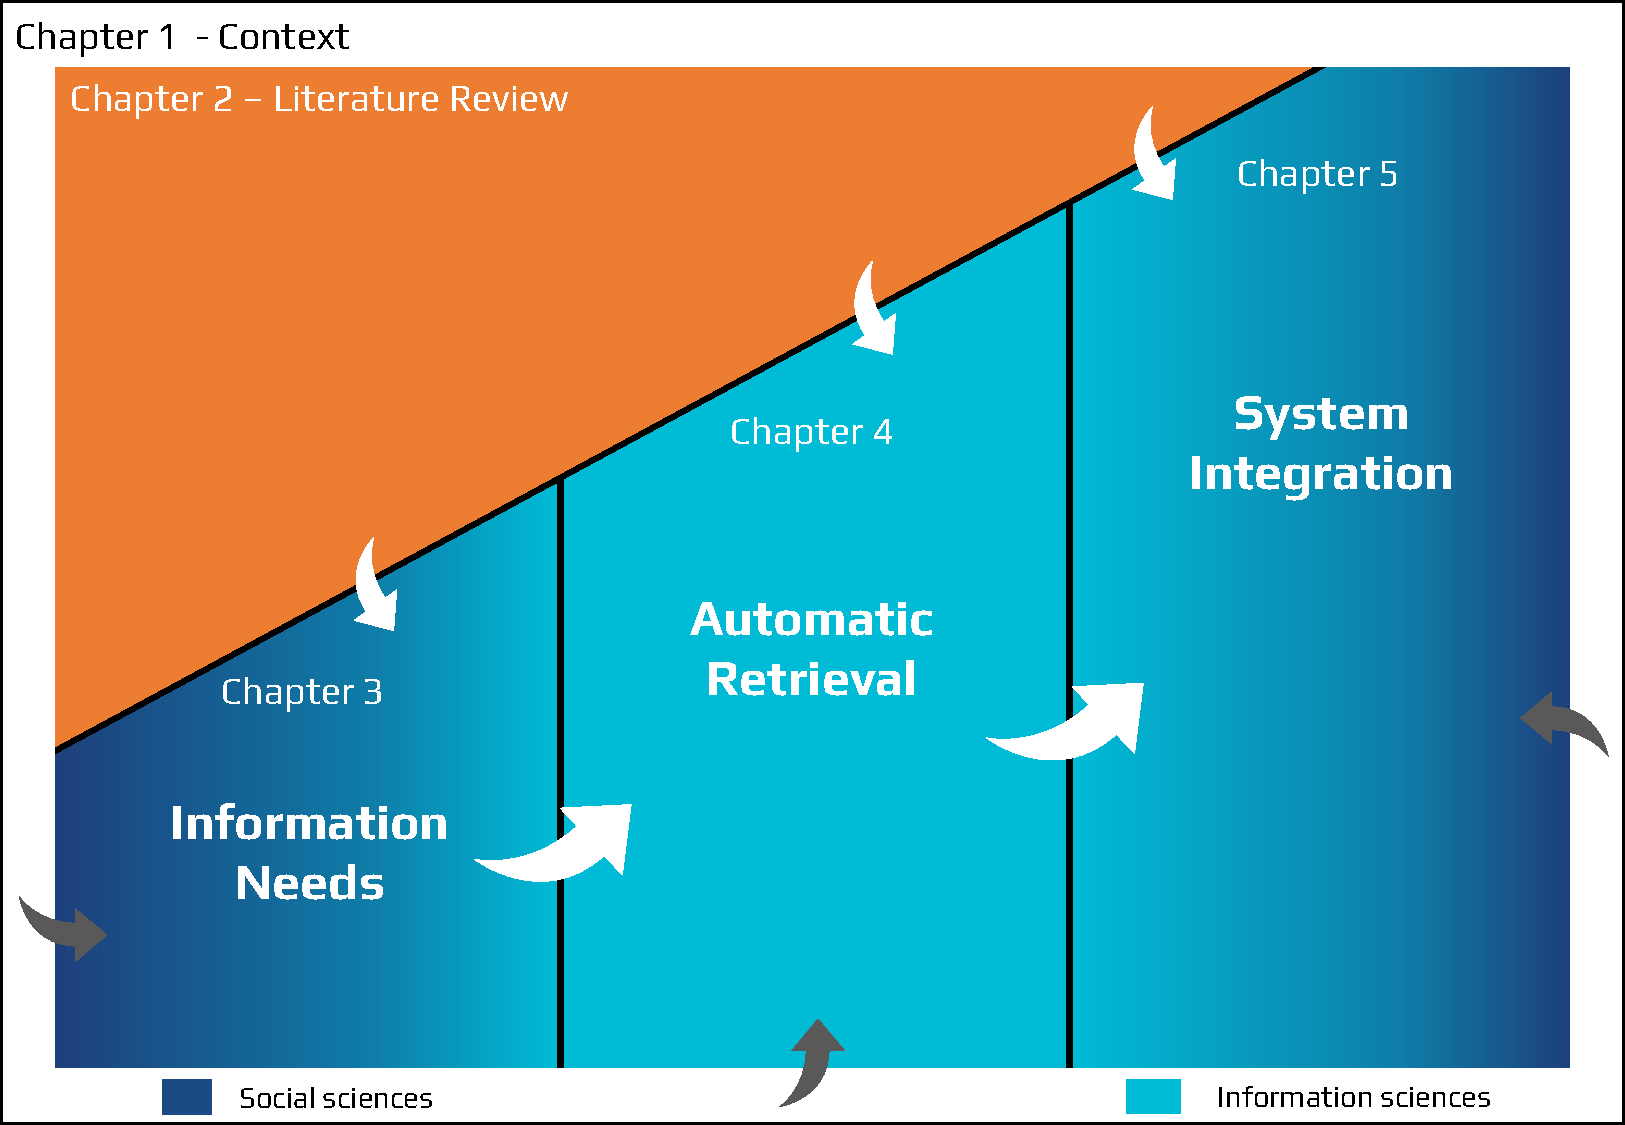
\includegraphics[width=0.92\textwidth,keepaspectratio]{figures/chap-0/big-picture.pdf}
    \caption{Overall organisation of the document. The arrows indicate the contribution of each part on the others.}
    \label{introduction:big-picture}
\end{figure}

%%% Local Variables:
%%% mode: latex
%%% TeX-master: "../ma-these"
%%% End:


\chapter{Context and problematic}

\section{Crisis management domain}
\subsection{A definition?}
Defining the concept of crisis provides a hint of the challenges that lie within this domain.
Although the term is widely adopted in everyday language, it is paradoxically difficult to provide a precise and definitive scientific definition.
The term is used every day for both financial crashes and natural or humanitarian disasters.
Many researchers have tried to define this vague concept.
In 1994, \textcite{lagadecGESTIONCRISES1994} identified numerous attempts of definitions.
Taxonomies such as the one proposed by \textcite{rosenthalCrisisDecisionMakingNetherlands1986}, who, wishing a broader definition of "crisis", were interested in the different types of crises.
They then proposed the following taxonomy:

\begin{itemize}
    \item The "unimaginable" crisis, requiring that we really question the unthinkable (it does not appear very frequently).
    \item The "neglected" crisis.
    \item The "almost inevitable" crisis, in spite of a preventive action.
    \item The "compulsive" crisis, which results from inadequate management.
    \item The crisis sought by some, internal or external, actors.
    \item The crisis deeply desired by all parties.
\end{itemize}

In an almost similar way, \textcite{mitroffStructureManmadeOrganizational1988} proposed a classification of crises according to intrinsic characteristics.
The authors use a 2D matrix to classify the different types of events.
One of the components opposes the origin of the event (internal or external) while the other axis opposes the "social" or "technical" aspects.
For instance, company bankruptcies are located in the internal/technical quadrant, terrorist attacks in the external/human quadrant or natural disasters in the external/technical quadrant.
Brief definitions have also been proposed to define the term itself.
\textcite{hermannIssuesStudyInternational1972} proposed that "a crisis is a situation that threatens the essential goals of the decision-making units,
reduces the time available for decision making, and whose occurrence surprises those in charge".
More than a simple situation, \textcite{rosenthalCrisisDecisionMakingNetherlands1986} will prefer to insist on the notion of crucial decision making.
Thus, "A crisis is a serious threat affecting the basic structures or the fundamental values and norms of a social system,
which - in a situation of high pressure and high uncertainty - requires crucial decisions to be made."
But crises are also periods of uncertainty and disarray of organizations, where rules and processes are blurred.
\textcite{lagadecGESTIONCRISES1994} somewhat abandoned the notion of succinctness by proposing a more ambitious definition through a higher level viewpoint.
Thus a crisis is "a situation where multiple organizations, facing critical problems, subjected to strong external pressures, bitter internal tensions, are suddenly and for a long time projected on the front of the scene;
all this in a society of mass communication, that is to say "live", with the assurance of being on the front page of the radio news.

From the definitions given above, one can see the difficulty of defining the concept of crisis, as it is so diverse.
Crisis situations, although they appear to be a constant in our societies, seem to be out of reach due to the lack of regularity in the concept.
In the end, crises seem to be the demons living in the dark face of our societies.
Invisible and seemingly out of reach, we are only witnesses of their sudden and brutal irruptions in the visible phase of our world.
In fact, these irruptions invariably result in an eruption of chaos.
This metaphorical representation translates my personal vision of what a crisis is and the inherent complexity of the definition of this concept.
But while describing those "demons" seem an incredibly difficult endeavour, the irruptions themselves and their consequences possess common points.
Theses common points are the caracteristics discussed in the following.

\subsection{Some caracteristics of a crisis}
It now appears that a quantifiable and fixed definition of the concept of crisis is difficult to achieve.
However if the concept of crisis remains vague, the effects and consequences are real and quantifiable.
Victims, material damages, environmental destructions and other more or less reversible consequences are tangible and known by all.
A first characteristic that can be extracted from the previous definitions is the emergence of chaos that creates a brutal rupture.
Crises are thus to be distinguished from incidents, which are difficulties for which preventive measures allow to keep the situation under control.
In the absence of a definition, having an overview of the multi-dimensional consequences of crises is an important step in building an adequate representation of the concept.
The literature is rich in numerous efforts to inventory the manifestations of crises.
Many authors, sharing the observation that it is difficult to define the phenomenon, even propose to define crises based on their consequences.
Thus, for \textcite{milburnManagementCrisis1972}, only an event that meets certain criteria would be eligible for the title of crisis.
The characteristics they evoke are:

\begin{itemize}
    \item Threat to assets identified as essential by managers.
    \item Need for quick decisions.
    \item Relatively short time frame for response.
    \item Lack of emergency measures available, since it is an unforeseen situation.
    \item Need for innovation in solving the problem, due to the absence of a pre-existing system.
    \item Information overload.
    \item Ambiguity.
    \item Increase in the number and importance of requirements.
    \item Internal conflicts in the organization.
    \item Considerable fatigue.
\end{itemize}

This approach is discussed by \textcite{rosenthalCrisisDecisionMakingNetherlands1986}.
The latter put forward the problem of defining where to stop taking into account the effects of the crisis.
They consider that the previous list of limits does not sufficiently take into account all the facets of the crisis and in particular the opportunities that are created by such an event.
However, this first attempt to identify the characteristics of the crisis allows to identify certain characteristics.
In a similar approach, \textcite{finkCrisisManagementPlanning1986} define crises as situations that expose to risks.
Among the risks that identify we find the risk of:

\begin{itemize}
    \item Escalate;
    \item Attract significant media and administrative attention;
    \item Affect the normal operation of the company;
    \item Call into question the public image of the firm and its leaders;
    \item Reach the very foundations of the organization.
\end{itemize}

In the light of the two previous authors, \textcite{lagadecGESTIONCRISES1994} summarizes these caracteristics through three main caracteristics:

\begin{itemize}
    \item Surge: A crisis is a tsunami. Information, issues, external actors involved, media attention etc.
          Regular processing capacities are overwhelmed as everything is tenfold.
    \item Disruption: The universe in which the organisation/system was is falling appart. Allies are disengaging. New, unusual actors (and most ofen, unwanted) appear.
          An overall ambiguity is cast onto the system hit.
    \item Breakdown: The system is falling appart. The regularity is not anymore. All reference points both internal and external are disappearing.
          All the decisions are "no-win" for the organization.
\end{itemize}

These caracteristics are provided using a high level point of view and encapsulate a lot of concepts.
But they provide valuable information to create a big picture of what a crisis is.
In a different fashion, \textcite{fertierInterpretationAutomatiqueDonnees2018} proposed caracteristics that pave the way to a quantification of crisis events:

\begin{itemize}
    \item Geographic scope of the event.
    \item Duration (time between the first and last consequences, including replicas).
    \item The \emph{severity} of the event (minor/major). Scale established according to the number of victims and or material damage.
    \item The \emph{complexity} of the event, depending on the number of dimensions involved in the event, the number of layers and replicas of the crisis.
\end{itemize}

These criteria can be used as metrics to rank different events according to the impact they had.
Theses various caracteristics built over time highlight the diversity of consequences following a crisis event.
Caracterizing such events definitely benefits from a multidisciplinary approach, as different viewpoints lead to a different picture of the phenomenon of crisis.
The next paragraph presents the different terms used in this dissertation and provides the
semantic associated with them.

During nominal times, the \emph{population} lives in an \emph{environment} in which exist \emph{systems} composed of valuable \emph{assets} managed by \emph{organizations}.
Usually, when one studies a crisis, the point of view of an organization is taken.
The environment refers here to everything that is outside of the system or organization of interest.
The close environment can be composed of other assets part of other systems or organizations.
It can be other companies, other cities, other countries etc.
In the environment there are systems and their associated organizations that are impacted.
The part of the population that suffers from the event are considered as the \emph{victims} of the event.
Among all these systems, there is one of particular interest when a crisis happens: the crisis management system, which is in charge of the response to the event.
At crisis time, the organization in charge of crisis management creates a \emph{crisis cell}.
The United Nations Department of Humanitarian Affairs defines a crisis cell as "a facility officially designated for the direction and coordination of all actions in the response phase of a crisis".
The crisis cell is composed of \emph{operators} that gather, filter and share incoming information to the \emph{decision makers}.
The decision makers make \emph{decisions}, some of which are instructions to the \emph{response teams}.
A crisis has an effect on all the elements of the framework created above.
Using the created framework, one can see how the different characteristics mentioned above are positioned.

\subsubsection{The environment}
The first concept is the concept of environment.
The environment represents an area.
When an event hits, the environment can be splitted in two parts.
A part that is impacted by the event (the crisis environment) and the part that is not.
There are different kinds of crises, depending on the geographic scale of the event.
Some events can concern only a small industrial area, as in the case of water polution for instance, or have a worldwide scale, as in the case of the global pandemic that the world is facing at the time of writing this document.
Events with different scales involve actors accordingly.
A crisis can affect the environment in which systems and organizations exist in several ways.
But the main caracteristic effect is the sudden realization that the environment that decision makers were used to seems to have simply disappeared.
Infrastuctures, resources or actors that were supposed to be available are not anymore, or worse, their status are unknown to the decision makers.
Crises reshape the environment and consequently, the first steps taken once the organization realised that they lost control of the situation, is to figure out what this new environment looks like.
But not only the environment of the system is reshape, but the system itself is too.

\subsubsection{The system}
A system consists of: i) an organization in charge of the system and ii) issues that it considers important.
In fact, a crisis affects a system if and only if the system's stakes are threatened.
As an example, one can imagine the differences between a volcanic eruption near a city versus a volcanic eruption in a desert.
The former would be a dramatic event while the later would probably modify a few air traffic lanes.

Crises often result from the combination of different factors.
The organization in charge of the systems is supposed to protect the known vulnerabilities of the system and prepare for the unknown ones.
A crisis can emerge from a stressing event on one of those vulnerabilities.
To illustrate those interactions, \textcite{benabenCollaborativeSystemsCrisis2014} propose a framework which illustrates the relation between the different concepts Figure~\ref{context:fred-framework}.
The consequences are, according to the previous authors, the result of an event on risks (which we call here vulnerabilities).
These risks are in their turn the result of dangers on stakes.

\begin{figure}
    \centering
    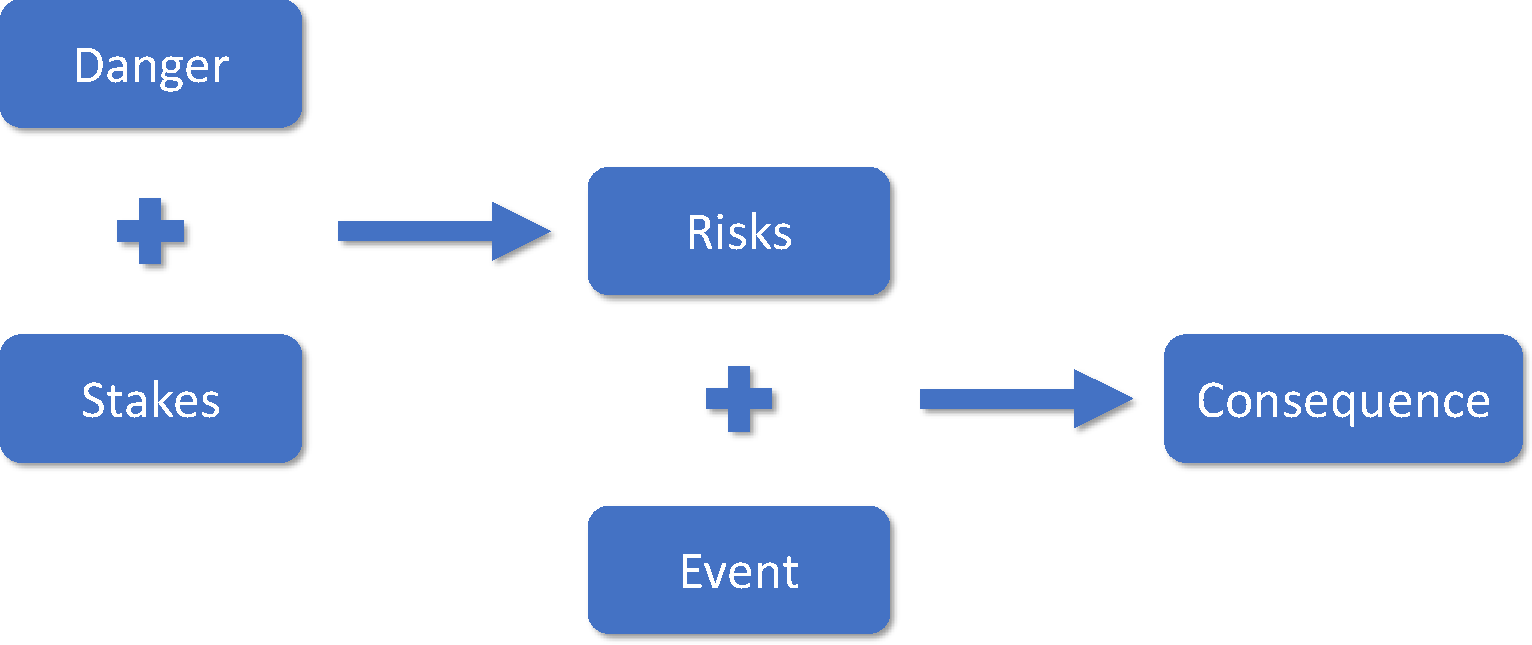
\includegraphics[width=\textwidth]{figures/chap-1/fred-consequences-framework.pdf}
    \caption{Crisis causality chain from \textcite{benabenCollaborativeSystemsCrisis2014}}
    \label{context:fred-framework}
\end{figure}

Each consequence can in turn become a danger or an event that endangers the system.
\textcite{fertierInterpretationAutomatiqueDonnees2018} puts forward this phenomenon through what it names "the cascade effect".
The crisis is self-feeding with the dynamism explained before and drags the system in its fall.
The best known industrial example is undoubtedly the Chernobyl nuclear disaster.
The cascade effect also joins the "surge" evoked by \textcite{lagadecGESTIONCRISES1994}, which is based on numerous testimonies of people who were involved in the crisis management.

In the end, a complete disruption of the system occurs.
Normal operation is no longer possible. The existing processes are no longer valid.
The historical partners are no longer available while unusual actors appear.

The consequence of this disruption is the increase in complexity of the operations.
Additional precautions are required for each decision and intervention that follows.
Every action that was once trivial becomes uncertain.
Most of the usual signals have disappeared and the remaining ones are ambiguous.
At the same time, the information requirements for each decision explode.
The intact parts of the system freeze into inaction.

\subsubsection{The organization}
The organization is the group of individuals that compose and manage a system.
The employees of a company, the first responders, all of them compose the organization with respect to a hierarchy between the different members of the organization.

The organization during the crisis is in charge of responding to the event.
It must protect the system and especially the assets.
In this sense, the organization can prioritize the value of the assets.

The activation of the response depends on how long it takes the organization to realize that the event is there.
There may be a lag time between the first effect of the crisis and the activation of the response.
By the time the response is activated, the crisis has already impacted a significant part of the system and its state is therefore altered.
This change in the state of the system plunges the organization into uncertainty and doubt.
The system is no longer in a known state.
The situational awareness has changed and there is an urgent need to re-establish a coherent vision for further response operations.
The situational awareness of an organization and its impact on the response are further developed in chapter 2 of this manuscript.
Then begins the reclamation of information for the organization.
From this point on, every decision made is crucial, to protect the stakes.
But with the loss of knowledge about the state of the system, every decision comes with a lot of uncertainty.

To reduce uncertainty, the organization will seek to know the state of the system.
It therefore requires reports on all aspects of the system.
The organization is successively drowned under two consecutive waves.
The first one concerns the feedback of information on the different dysfunctions and limitations that have appeared.
The second wave is about reporting on the state of the environment and the system as a result of the need to regain visibility for decision making.
This reporting may be partially automatic for automated systems and if the sensors have not been influenced by the crisis.
For emergency services (911, firemen), this feedback is essentially done via the response units deployed and the calls of the impacted people.
Similarly, external services (meteorological, specialized...) can also provide external data to help the organization make decisions.
However, the organization is rarely prepared to handle so much information and the organization becomes overwhelmed.

In addition to this, the initial information feedback is scattered and therefore ambiguous.
The context in which each piece of information fits is absent or limited.
The situation faced by the organization can be illustrated with a puzzle.
However, we do not know the final outcome of the puzzle and the pieces are provided to us one after the other, in no particular order.
We are also forced to place the pieces of the puzzle (i.e. make decisions) without having the following pieces.
Under these conditions, it is only possible to complete the puzzle when enough pieces are provided.
To imagine the psychological consequences of such a way of completing the puzzle makes it obvious why we don't do puzzles in this way.

In addition to these internal difficulties, there is also the external pressure.
The event inevitably attracts the attention of regulators, higher authorities and the media.
The organization, sometimes unknown until then, finds itself under the spotlight.
Its past is scrutinized, looking for previous mistakes that may have led (or not) to the current event.
Its leaders and their decisions are dissected and the inconsistencies are highlighted as soon as possible in order to feed the headlines.
Thus, in addition to the physical impact of the crisis, the trust and the image of the organization is also weakened.

\subsubsection{The decision makers}
The decision makers are the people with responsibility in the organization.
Most of the organizations are hierarchical.
In fact, there is also a hierarchy of decision makers.
The decisions of some individuals thus take precedence over those made by their subordinates.
Of course, at the time of a crisis, this phenomenon increases tenfold, adding to the already existing confusion.

Moreover, all the decisions look like "no-win" for the organization.
The problems pile up without them having time to solve any of them.
The knowledge of the whole they are in charge of has suddenly disappeared as well as the assurance it gave them.
Their perception is distorted, as much as their assumptions, and each new decision is a disappointment that slowly leads them to realize that there are no more good decisions, only fewer bad ones.
Of course, all this is done in a hurry, created by the influx of requests and reports.
Decision making is further complicated by the fact that the usual processes and safeguards they used to rely on potentially no longer exist or have become irrelevant.
Improvisation and innovation, once feared, is now required with the realization that inaction will be as, if not more, costly than action.
The stress on the organization is hitting decision makers hard.
Under the urgency, stress and fatigue, every decision becomes a battle to be fought in this war that the crisis has created.

This first part of the chapter presents my vision of the crisis and what it implies.
This vision will drive the manuscript, including the structure of the different concepts affected by a crisis - the environment, the system, the organization and the decision makers.
The reminder of this section develops how organizations deal with these situations.

\subsection{Crisis Management}
Crises are not a question of "if" but of "when".
This inevitability implies an upstream reflection on the part of organizations and a consideration of this problem within the systems.
These practices are called crisis management.

Wikipedia defines crisis management as "the set of organizational modes, techniques and means that allow an organization to prevent,
prepare for and respond with the occurrence of a crisis, and then to draw lessons from the event to improve procedures and structures
with a forward-looking vision" (Wikipedia, 2021).
This definition perfectly highlights two main characteristics of crisis management.
First, crisis management is more a broad spectrum methodological toolbox than a set of recipes to be applied in case of an event.
Secondly, it takes into account the different temporal phases of the crisis.
In the following, we detail these two aspects.

\subsubsection{The crisis management cycle}
The crisis management literature identifies four major phases.
These phases are most often represented in the form of a cycle.
The cycle illustrates the inevitability that we mentioned earlier. (put the references).
The 4 phases are :

\begin{itemize}
    \item Prevention : phase aiming at preventing the appearance or reducing the effect of an emergency situation.
          This phase consists of identifying potential hazards that threaten system vulnerabilities and appropriate measures.
    \item Preparedness: Measures that facilitate the response to the disaster. It involves ensuring that resources are available and deployable, that response personnel are trained, and that the potentially impacted organization is psychologically prepared.
    \item Response: corresponds to the activation of measures "is engaged from the beginning of a major event, to take cognizance of the situation, go to resources, make decisions
          and follow up on actions in progress".
    \item Recovery: Phases that follow the response to the crisis. It corresponds to the repair/reconstruction of the parts of the system impacted by the event.
          This stage is often accompanied by an analysis of the risks associated with the repairs, in order to avoid creating a replica of the crisis.
\end{itemize}

In this cycle, only one transition between two phases is clear: the one between preparation and response.
This transition occurs when the organization acknowledges the event and goes into crisis management.
The other transitions correspond more to a duration where two phases coexist.
The prevention phase, however, leads to some debate.
\textcite{benabenCollaborativeSystemsCrisis2014} argue that the prevention phase is, in fact, common to the whole cycle.
Even during the response and the recovery, the organization observes prevention measures to prevent cascading effects.
If prevention is common to the whole cycle, the cycle can be simplified with only three phases in crisis management: the preparation (before the event), the response (during the event), the recovery (after the event).

Also, it is possible to see beyond the cyclic representation.
Today's world is complex, tense and deeply interconnected. % Reference?
As a result, large organizations or countries possess a large surface vulnerable to potential disruptive events.
Then, instability and crisis management somehow become the norm.
Small and large incidents trigger responses from the organization.
However, these events are concurrent to each other and each one is at a specific phase of the cycle.
Consequently, looking at the global picture, these organizations are dealing with multiple crises at the same time.
Similarly, large crisis situations are often not dealt at the global level directly.
A local firefighters station will not deal with a hurricane by itself for example, but rather will take care of smaller, local events that are the direct consequences of the hurricane.
Here again, the hurricane triggers the response phase in the cycle, but one could zoom into this phase and see that there are in fact many smaller and concurrent cycles happening at the same time.
The cycle representation of crisis management does not account to the scale nor the complexity of events, but it is a good enough abstraction to represent the different times in an event.

\subsubsection{Stakes in Crisis Management}
As said before, crises threaten stakes of a system.
Crisis management is the tool used to oppose crises and composes one of the systems present during a crisis situation.
This system has its own stakes during an event.
As a result, the crisis management system faces problems that vary depending on the phase of crisis management the system is in at any given time.
Numerous authors from the information systems domain have studied these different issues and identified stakes.

During the response phase, \textcite[.~12--18]{fertierInterpretationAutomatiqueDonnees2018} identifies 5 stakes for the organization:

\begin{itemize}
    \item The collaboration between internal and external stakeholders.
    \item The situational awareness~\footnote{Chapter 2 of this manuscript is devoted to the meaning of "situational awareness" for an information system. For this reason we will not go into further detail here.} associated with the environement and the system.
    \item The data obtained during the event from different sources.
    \item The information acquired from the previous data.
    \item The system in charge of data and information processing.
\end{itemize}

\textcite{batardIntegrerContributionsCitoyennes2021} also identifies two of the previous stakes as the overarching stakes in responding to a crisis situation:

\begin{itemize}
    \item The knowledge of the situation
    \item Coordination of the various actors
\end{itemize}

From these two main stakes, the author then proposes four axes to protect those.

First, the management of the multiplicity of data sources.
Organizations in charge of crisis management are already used to taking into account several data sources.
Feedback from the field from the staff allocated to the response as well as phone calls from victims or witnesses of the event are commonly used.
However, new sources are emerging such as the Internet of Things and the various sensors that can provide interesting records regarding certain events.
The rapid and global development of social media is also a potentially interesting source of data \textcite{meierStrengtheningHumanitarianInformation2013}.
The opportunities offered by this data source are detailed in section 1.2.3.

Secondly, the automatic interpretation of these data to extract relevant information.
This information is then delivered in an adapted way to the decision makers \textcite{luokkalaDevelopingInformationSystems2014,vandewalleImprovingSituationAwareness2016}.

Thirdly, the management of information systems adapted to the crisis management context.
This information system is supported by an IT system, whose role is to facilitate the response.
This facilitation is enabled by delegating some of the tasks necessary to i) restore situational awareness and ii) coordinate actors to the IT system \textcite{benabenManagementCollaborativeBehavior2015}.

Fourth, the information system and the computer system must be adaptable.
This strong constraint results from the nature of crisis situations.
A crisis management system must therefore be able to detect changes in the situation and react to them in an adapted manner \textcite{barthe-delanoeEventdrivenAgilityInteroperability2014,charlesModelDefineAssess2010}.

These previous analyses, strongly oriented towards information systems, highlight key stakes during crisis management.

\begin{enumerate}
    \item An understanding of the current situation and state of the environement.
    \item The coordination of the actors, that needs to be fluid and orchestrated accordingly to the event.
    \item A system for collecting and organizing the available data.
    \item A system for managing the information extracted from the data, adapted to the context of crisis management and its users needs.
\end{enumerate}

This analysis allows us to succinctly summarize the needs of the actors during crisis management.
Thus, the organization responsible for crisis management must first restore its knowledge of the situation using the data available to it.
Secondly, it must manage the information obtained from these data in order to best coordinate its response with its internal and external actors.

\subsection{Tools for crisis management}
The previous section identified 2 main stackes from the information system point of view: the coordination of the actors and the restoration, then management, of the situational awareness.
The protection of these stakes by the system is of the utmost importance to allow an adequate response.
Tools and practives have been developed to help organizations in charge of crisis response to address those issues.

\subsubsection{Organizational modes}
The organization of the response is one of the components of the preparation phase.
During this phase, the different future actors of the response agree on the roles of each and their responsibilities during the future event.
For instance, in the response phase, the system dealing with the response uses a hierarchical organization, layered with crisis cells.
A crisis cell is a facility officially designated for the direction and coordination of all actions in the response phase of a crisis.
They bring together the decision makers of the organization who implement and direct the various actors to respond to the crisis.
Thus, the crisis units must have a high-level vision of the event, but also be close to the actors of the response they are managing.
Large-scale crises (mobilizing many actors or a large territory, for example) will undoubtedly lead to the creation of a hierarchy of crisis units.
While the "low-level" crisis units orchestrate the response, a "higher-level" crisis unit is responsible for transmitting information between the "low-level" crisis units and coordinating their responses.
In France, this hierarchy is composed of 5 levels:

\begin{itemize}
    \item European
    \item National
    \item Zonal
    \item Departemental
    \item County
\end{itemize}

Each of the crisis cells set up has its own specificities, depending on the actors who compose it.
However, all are constrained by the same need for collaboration \textcite{benabenAIFrameworkMetamodel2020,comfortCrisisManagementHindsight2007} and information \textcite{comfortCrisisManagementHindsight2007,endsleyTheorySituationAwareness1995}.
It is precisely the role of the information system to manage and exchange situation-specific information between the different actors.

\subsubsection{Techniques and Methods}
The organization mentioned above is only effective if the actors coordinate their actions.
This coordination requires the communication of information available to the different actors.
The organization's information system is in charge of this aspect.

Wikipedia \textcite{InformationSystem2021} proposes the following definition of information system.
"An information system (IS) is a formal, sociotechnical, organizational system designed to collect, process, store, and distribute information.
From a sociotechnical perspective, information systems are composed of four components: task, people, structure (or roles), and technology.
Information systems can be defined as an integration of components for collection, storage and processing of data of which the data is used
to provide information, contribute to knowledge as well as digital products that facilitate decision making."
This definition mixes the definition provided by \textcite{oharaManagingThreeLevels1999,piccoliInformationSystemsManagers2019,zwassInformationSystemDefinition}.
Thus, the organization's information system is the cornerstone of information management within the organization.
It can be digitalized or not, depending on the needs and practices of the organization, as it reflects how the information is processed in the physical organization.
The information system is an abstract concept that encompasses many aspects of the organization.
The development and maintenance of the information system is performed during the preparation phase.
During this phase, hardware and software must be deployed, tested and used for training to ensure smooth operation during the response.
The hardware aspects are outside the scope of this manuscript, which is mainly interested in the software and social part of the information system Figure~\ref{context:information-system}.

\begin{figure}
    \centering
    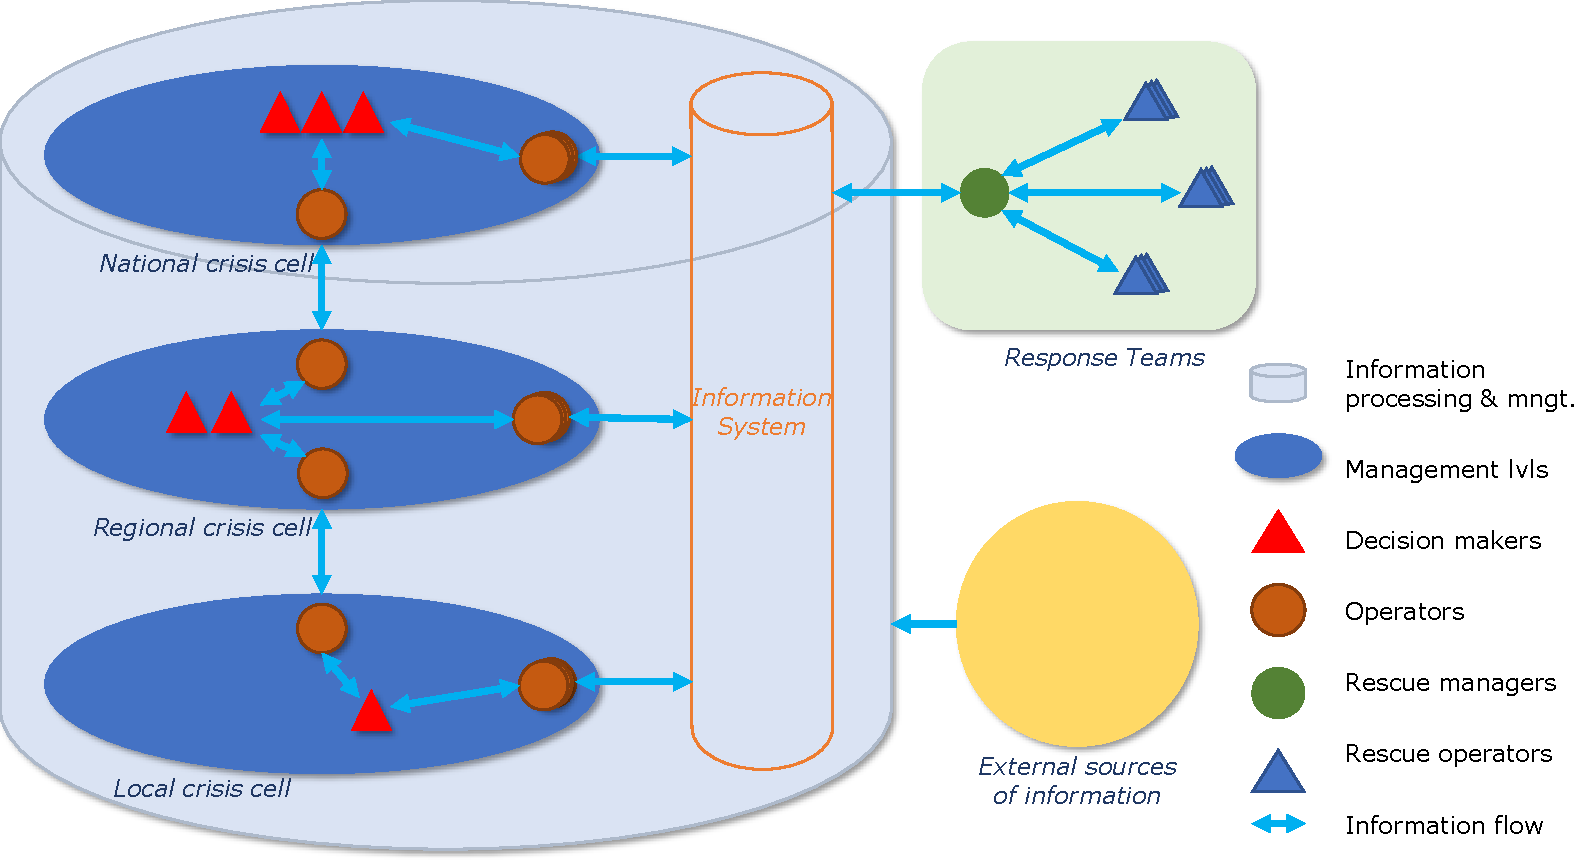
\includegraphics[width=\textwidth]{figures/chap-1/information-system.pdf}
    \caption{Representation of a crisis information systems and its interaction with the different members of the organization}
    \label{context:information-system}
\end{figure}

The role of an information system is, according to the definition, to collect, process, store and distribute information.
The information system is thus fed by data sources.
In France, \textcite{morelEtudePriseDecision2010} indicate that fire department services mainly receive their data from three sources:

\begin{itemize}
    \item The calls that victims make from emergency numbers.
    \item The crews deployed to respond to the crisis.
    \item Other organizations involved in crisis management.
\end{itemize}

The rest of the manuscript assumes that these data are common in most of the emergency services activated during the response to an event.

The previous part detailed the way crisis cells are organized in crisis response, and the hierarchy built to scale decision making with the size of the event.
Each actor of this hierarchy comes with its own, internal information system.
However, to enable the coordination between all the different actors, information has to flow between each of them.
Yet, two challenges arise.
First, the actors have to share a common vocabulary in order to communicate.
Secondly, the information system has to be designed to allow communication.

The distribution of information is often hampered by misunderstandings between the different actors.
The latter often have different skills, responsibilities and roles.
Each actor therefore builds his own vocabulary, his own terminology to designate the elements in his field of action.
If this facilitates daily operations, during an event, it complicates the collaboration and communication between the actors \textcite{opachMapbasedInterfacesCommon2020}.
The preparation phase is therefore an opportunity to identify the actors who will potentially be brought to collaborate during an event, and to bring them together so that they are familiar with each other's culture.

Common format and representations of the information between all the actors is needed to build a common understanding of the situation.
From a technical point of view, the different actors can decide to set up a "Commission Operational Picture (COP)".
According to \textcite{UnitNIMSCommunications}, a COP is "A representation that is established and maintained by collecting, collating, synthesizing and disseminating information among the different participants.
It allows the different actors to have access to the same information regarding the availability and location of resources and the status of different requests for assistance".
Thils representation is often cartographic, allowing the geographic component of an information to be easily represented.
Geographic information is also information that is equivocal among all actors.
The COP is therefore a tool that allows to initiate and build a dialogue between the different actors of the response.
It is also the visible face of the information system.
The COP benefits from all the advantages that the rest of the information system provides.
The COP can be automatically fed with the above mentioned data.
Thanks to this data, the information system can then produce useful information for the decision makers, and make it available automatically on the COP \textcite{fertierInterpretationAutomatiqueDonnees2018}.
One of the problems currently faced by COPs is their inability to communicate with each other most of the time, due to mutually exclusive software, which does not offer the possibility of dialogues between them \textcite{opachMapbasedInterfacesCommon2020}.

\begin{figure}[h]
    \centering
    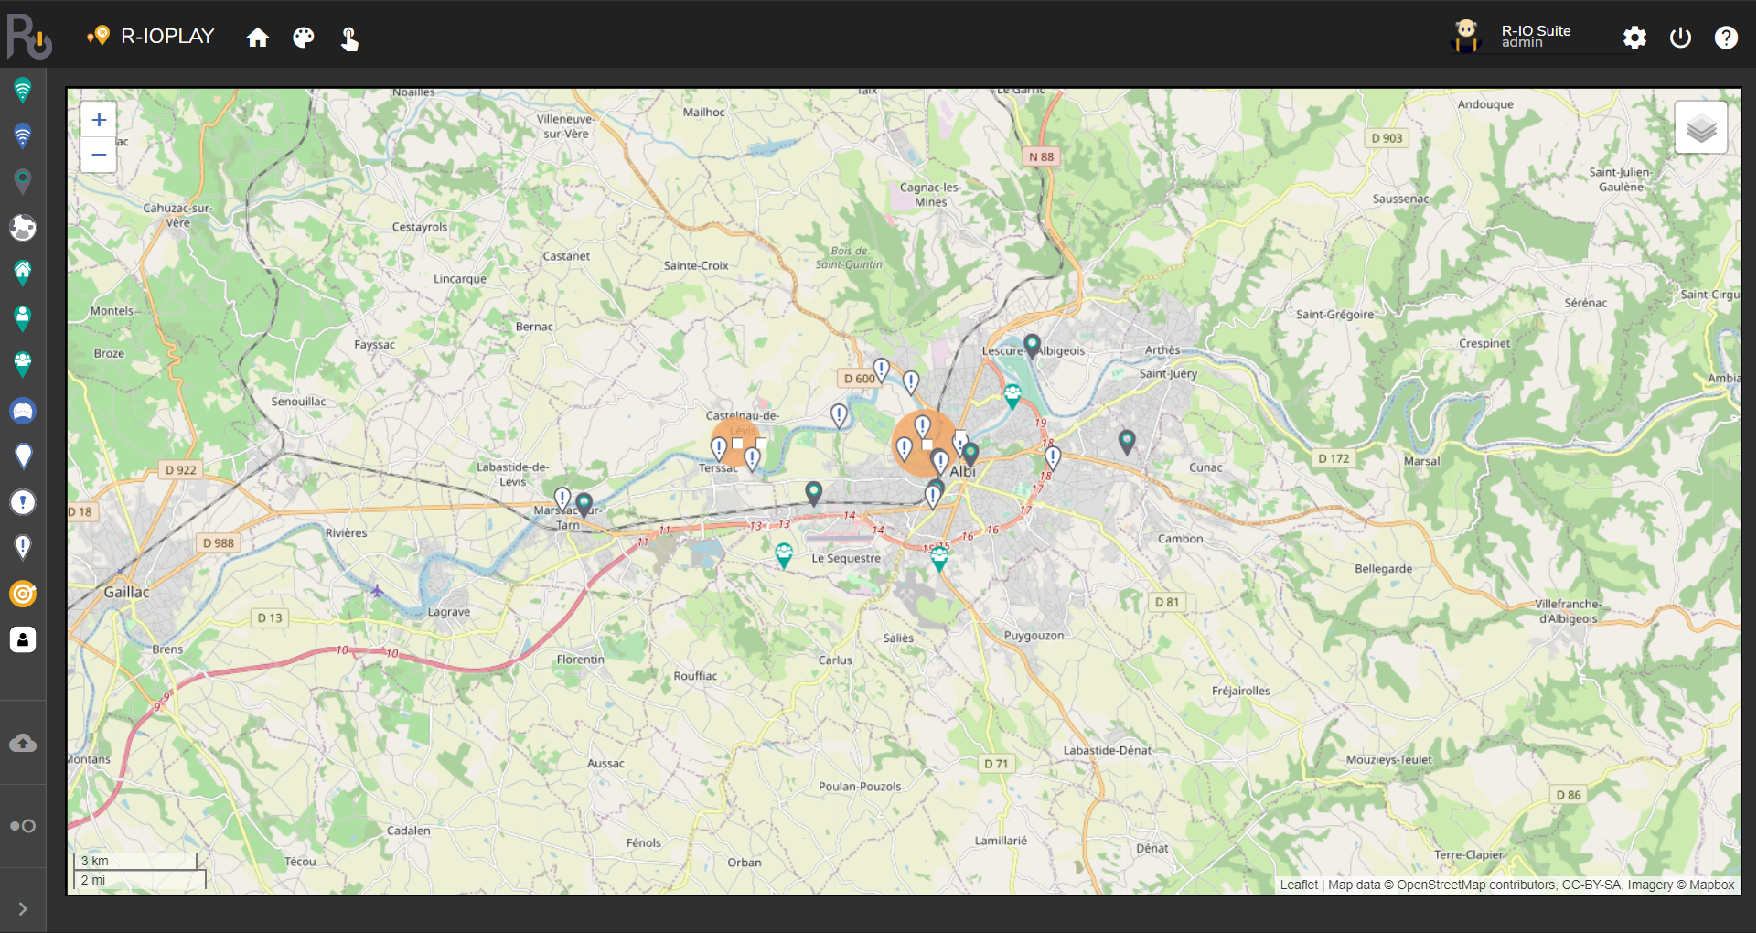
\includegraphics[width=\textwidth]{figures/chap-1/rio.pdf}
    \caption{Cartographic display of the R-IOSuite software in a flood scenario in France\protect\footnotemark}
    \label{context:cop}
\end{figure}
\footnotetext{https://research-gi.mines-albi.fr/display/RIOSUITE/Welcome}

Finally, the COP is an asset for building and maintaining adequate and shared situational awareness among all actors.
As we saw earlier, the restitution of situational awareness is one of the challenges of crisis management, as is the coordination between the different actors.
The COP is an asset because it is a tool that allows both issues to be addressed simultaneously.

Crisis management is a challenging domain.
By nature, crises events are uncertain and hard to define.
Yet, patterns emerged from this uncertainty especially when it comes to information management.
Regardless of the event, decision makers are in dire need of information about the impact of the event on their system and organization.
Tools and methodologies have then been developped to assist the decision makers from the different organizations in coordinating and understanding the situation.
Research and development  around digital tools to support information management takes place in the crisis informatic domain \textcite{palenCrisisInformaticsHumancentered2020}.
One of those tools is the Common Operational Picture.
The COP is a map shared between the different actors, with common, but also specific information, displayed.
This representation is the visual face of a common information system used by all the actors.
However, the COP comes with its one challenge, as each individual information system has to be able to share information with the common one.
Also, the different actors have to agree on common representations and terminologies that will be used by the COP.

\section{Social media}
\subsection{What are social media?}
In the previous chapter, we identified the informational needs of decision makers during crisis events.
At the same time, and somewhat paradoxically, our societies have never had so many means and platforms to exchange information.
Among these platforms, social media have recently appeared.
Social media are Internet platforms that appeared during the Web 2.0 era.
The term Web 2.0 was developed between 2003 and 2007, by T. O'Reilly.
This terminology was initially born to revive the economy of the Web after the explosion of the dot.com bubble formed during the development of Web 1.0 consisting mainly of web portals.
Web 2.0 reflects the development of the community web and is organized around platforms that allow their users to connect with each other in order to co-create and share content \textcite{oreillyWhatWebDesign2007b}.
Social media fits into this definition.
\textcite{kaplanUsersWorldUnite2010} identify 6 types of social media: blogs and micro-blogs (e.g. Twitter), social networking sites (e.g. Facebook), collaborative projects (e.g. Wikipedia), content communities (e.g. Youtube), virtual social worlds (e.g. Second Life) and virtual game worlds (e.g. World of Warcraft)

Social media are now essential websites and platforms that have up to one billion users in the case of Facebook.
Like the crises we mentioned earlier, it is difficult to grasp their full dimensions.
These platforms, often global, connect users from all over the world, forming a true digital double of our societies.
The multitude of cultures, communities, languages and codes that co-exist in a single place has no equivalent in the history of humanity.
The disproportionate size of these platforms is accompanied by opportunities and threats.
Social media are indeed a great gateway to the world, allowing to connect with an incredible number of people around the globe.
It is also an efficient way to share information and exchange with other users, through many formats.
If the majority of social media users are consumers of content, a significant portion of them also create content \textcite{fuchsSocialMediaCritical2021}.
The creation of content on these platforms is thus their cornerstone, so much so that some of these platforms do not hesitate to pay their users who contribute, thus making a new profession emerge: content creator.

But with this opportunity to unite humanity in a few hubs on the Internet, comes many challenges.
Spreading false information, harassment campaigns against individuals or state disinformation, feeding political disengagement or addictions are some of the problems associated with social media.
If all these problems are not exclusive to these platforms, their dimensions and dynamics amplify them greatly.
The rest of this section draws the reader's attention to two components of interest in understanding social media, namely what is a social network and what is viral information.
Other keys to understanding may be of interest as well, but for the sake of brevity these will be the only two mentioned in this manuscript.

\subsection{Some social media caracteristics}
\subsubsection{On the Social Network}
Most people live in a community.
Family, friends, neighbors, colleagues, all of these circles form an individual's social network.
The social network is an integral part of one's life.
Some researchers have looked into the question of what the social network of different individuals could look like.
Obviously, a network is a graph, and this question has a strong link with mathematics.

It is therefore not surprising that the first interesting results come from a mathematician.
By being interested in random networks, \textcite{erdosEvolutionRandomGraphs1960} discovers that each node of the network is on average separated from any other node by six intermediate nodes.
More surprisingly, this result is little affected by the size of the network.
It was not until a few years later that these results, which had until then been essentially theoretical, found a concrete application in the social sciences.
\textcite{milgramSmallWorldProblem1967}, verified the validity of the previous results within a population of individuals.
Each node then becomes an individual and the edges are the relationships between the different individuals.
Their results obtained in this physical experiment validated the theoretical results on random networks.
This property is now known as the "six degrees of freedom".

\textcite{wattsCollectiveDynamicsSmallworld1998} sought to deepen the understanding of the six degrees of freedom and discovered on this occasion the structure in small worlds of social networks.
So if people meet each other by chance as in Paul Erdös' model, the social network itself is rather composed of small communities, with many links between individuals
and very few links between communities.
This model is called "small world network", because, contrary to intuition, the majority of individuals in the network are connected by very few intermediaries, regardless of the distance between them or the community to which they belong.

Similarly, \textcite{barabasiEmergenceScalingRandom1999} deepens Paul Erdös' random model by discovering another property of social networks.
Indeed, the random model predicts that the distribution of the number of friends among individuals must follow, by construction, a normal distribution.
However, this is not what they discover experimentally.
The distribution of the number of friends among individuals follows a power law.
This property thus forms a scale invariant network, where individuals connect preferentially to the most influential nodes.

In reality, both models have their properties verified.
We can therefore consider, as a first approximation, that the two models coexist.
Therefore, a social network can be described through three main properties:

\begin{itemize}
    \item Each individual can be linked with only a few intermediaries (6 on average), whatever the size of the network
    \item The network is structured in communities that are very connected to each other.
    \item The communities are connected by a few individuals who act as hubs.
\end{itemize}

These properties are illustrated on Figure~\ref{context:social-network}.

\begin{figure}
    \centering
    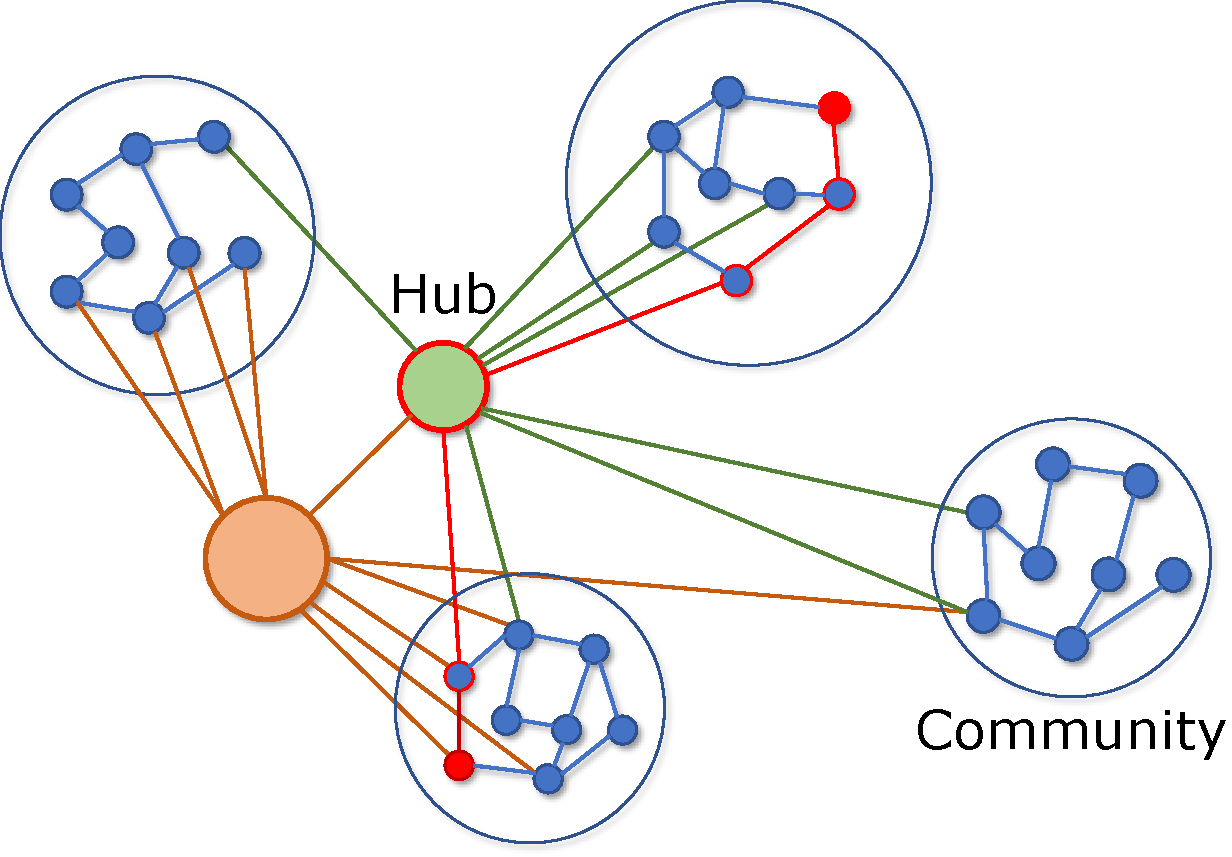
\includegraphics[width=\textwidth]{figures/chap-1/network.pdf}
    \caption{Illustration of the combination of both social network models from \textcite{wattsCollectiveDynamicsSmallworld1998} and \textcite{barabasiEmergenceScalingRandom1999}.}
    \label{context:social-network}
\end{figure}

These properties are valid whether the social network is "real" or virtual - many of the experiments in the previous publications were obtained by studying social media.
Thus, social media can be seen as a multitude of communities, linked together by hubs (influencers).
Having the structure of social networks in mind allows us to better understand the propagation of information within a social network.
This brings us to the next section, and a topic familiar to all social media users: viral information.

\subsubsection{On Virality}
The propagation of information, true or false, within a community is experienced daily by everyone.
However, this characteristic of information sharing is exacerbated in the case of social media for two reasons.
First, social media brings together a large number of users in one place.
Second, they provide their users with a number of tools that aim to make information sharing much easier.
By construction, social media put information and content sharing at the center of their strategy.
However, in a social network, each user can easily reach any user in very few intermediaries, regardless of the size of the network.
Moreover, information can quickly reach a very large number of users if it is shared through network hubs.

This speed of dissemination is thus unusual, as are the results that such propagation can generate.
Research teams are therefore interested in understanding what viral information is and how this virality is characterized.
By studying chains of information propagation, they identify that the phenomenon of virality is quite rare.
Large content cascades are the exception, not the rule.
99\% of posts are reposted less than 10 times, while cascades of more than 1,000 reposts are created by 0.001\% of the posts.
Viral content is therefore rare, but when it goes, it is seen by a large number of users.

Recently, the notion of virality on social media has been widely associated with the term "fake news".
Fake news are a concern that grew with social media platforms themselves.
Particularly, in the 2016 US election context, the involvement of Russia in the process through disinformation campaigns~\footnote{https://www.judiciary.senate.gov/meetings/extremist-content-and-russian-disinformation-online-working-with-tech-to-find-solutions}
brought even more attention to that problematic.
\textcite{lazerScienceFakeNews2018} define fake news as a "fabricated information that mimics news media content in form but not in organizational process or intent".
The authors warn about the stakes and threats posed by fake news on our societies and call for more efforts to understand these dynamics, which are still largely misunderstood.
Also, viral content cascades depend on the veracity of the content they propagate.
Thus, false information spreads faster, to more people, for longer with an essentially vertical structure (friends of friends relay the information).
On the contrary, real information spreads more slowly, to fewer people, with slower kinetics and an essentially horizontal structure (the information is essentially shared by the sender's followers).
Deriving from the previous results, \textcite{vosoughiRumorGaugePredicting2017} built a system that assesses the veracity of one piece of information, based on the way this information is propagated.
Their method achieves a classification score of 75~\% using only this simple feature.

Finally, the understanding of the propagation of information on social media remains largely marginal.
The call to link more independent research to the platforms of \textcite{lazerScienceFakeNews2018} remains largely anecdotal, effectively hindering progress in this field.
In the following section, we explore, in light of the few elements presented so far on social media, the different opportunities for crisis management.

\subsection{Opportunities and threat posed by social media for crisis management}
The previous sections highlight the digital double role of the social media society.
These platforms offer a point of view never seen before

Important events have long had an imprint on the Internet.
In the aftermath of the September 11 attacks in New York, web pages for exchanging information about people were created \textcite{palenCitizenCommunicationsCrisis2007}.
The relationship between crisis events and social media is now well established.
The case of the ditching of the U.S. Airways Flight 1549 on the Hudson River in New York City in January 2009 is often used as an example of the impact that social media can have in important situations.
The information of the ditching had indeed been relayed on social media before all the traditional media \textcite{murthyTwitter2018}.
Other studies have highlighted the reaction of social media during crisis situations, as in the case of tornadoes in the United States \textcite{justinei.blanfordTweetingTornadoes2014}.

However, crisis management requires data and information to be able to achieve its objectives.
Social media appear as a potential source of information for emergency services \textcite{tapiaSeekingTrustworthyTweet2011}.
Moreover, where phone calls were the only link with the population, this digital twin of society offers a real time overview of the conversations and feelings of the people who are affected by the event.
These platforms thus make available a wide variety of data, which can help emergency services.
As content creation platforms, users can use the wide range of tools at their disposal to share information about the ongoing event.
Texts, photos and videos can help crisis decision makers to better understand the event, even in places where they have no resources deployed.
Social media can also bring back information that may have been missed by other actors within the organization.
Finally, users of these platforms not directly impacted may decide to help the victims.
These volunteers, digital or not, could be mobilized to assist the emergency teams deployed on the scene of the event \textcite{batardIntegrerContributionsCitoyennes2021}.

The full potential of social media is yet to be discovered.
However, these platforms come with challenges.
As mentioned in the previous section, fake news is a current problem with social media \textcite{lazerScienceFakeNews2018,vosoughiSpreadTrueFalse2018,oshikawaSurveyNaturalLanguage2018}.
This phenomenon is also mentioned in crisis management and attracts some interest from the scientific community \textcite{starbirdExaminingAlternativeMedia2017,sellMisinformationUSEbola2020}.
However, while misinformation and the sharing of false information is something we see on social media in crisis situations, it is not necessarily indicative of their uses alone.
\textcite{bubendorffConstructionDisseminationInformation2021} indeed highlights the small amount of information involved and the self-correcting effect of the crowd, which ultimately reduces the impact of false information.
Despite this, emergency services remain cautious about the use of information from social media.
By focusing on the use of social media by the latter, \textcite{tapiaGoodEnoughGood2014} also highlights their fears, which the authors believe are unfounded.
Because one of the main challenges of social media still lies in their relative novelty and the lack of understanding of their universe.

Social media are Internet platforms that provide content creation tools to their users, allowing them to generate and share data.
Altogether, Twitter, Facebook, Reddit, Instagram, Youtube and many others, have billions of users worlwide who share their everyday life, creations and feelings with their communities.
These digital twins of the society are ressourceful and possess valuable information for crisis management.
However, the dynamic of these platforms remain hard to understand for individuals and, in light of the recent controversies that have sprung, many are questioning their utility to ease crisis response.

\section{Natural Language Processing}
\subsection{On Natural Language Processing}
"Computational linguistics, also known as natural language processing (NLP), is the subfield of computer science concerned with using computational techniques to learn, understand, and produce human language content." \textcite{hirschbergAdvancesNaturalLanguage2015}."
As "learn, understand, and produce human language content" is a broad objective, the field is subdivided into major tasks :
Some of these tasks are:

\begin{itemize}
    \item Language recognition
    \item Machine translation
    \item Sentiment analysis
    \item Question answering
    \item Text summarization
\end{itemize}
The rest of this section presents the concepts and terminologies used in NLP.

NLP is concerned with textual data.
There is no lack of such data, as this format is used extensively to share information on the Internet (wikis, emails, messages, etc.).
To a computer, text is a sequence of ASCII or UTF-8 entities, called \emph{characters} in the format of bytes (or eight bits).
A set of textual data is called a \emph{dataset} or a \emph{corpus} (both terms will be interchanged thoughout this manuscript).
Corpora are most of the time composed of two parts: the \emph{metadata} and the text itself.
Metadata provide the context in which the data exists (e.g. a timestamp, recipient, receiver etc.)
The text in the corpus can be \emph{tidy} or \emph{raw} and in the latter case, will require a step of \emph{preprocessing}.
The characters in the sequence are grouped in units called \emph{tokens} during a process called \emph{tokenization}.
Tokenization depends on the language.
Western languages can split tokens using white-spaces or punctuation, but this way of splitting text can't be used for Japanase (that do not contain any space) or Turkish (as an agglomerative language) for instance.
Contiguous multitokens are called \emph{spans} and are used to represent high order tokens for specific tasks such as \emph{chunking} and \emph{named entity recognition}.
For instance, in the sentence "Bob scored a goal", we might want to extract the noun "Bob" and the verb "scored".
Named entity recognition aims at a similar objective, but with \emph{named entities}, a string mention of a real-world concept such as locations, organizations, persons etc.
All the unique tokens form the \emph{vocabulary} or \emph{lexicon} of the corpus and individuals are called \emph{types}.
These types can be either \emph{content words} or \emph{stopwords}, the latter being mostly used for grammatical purposes rather than for conveing information.
Also, words have one or more meanings.
The \emph{senses} are all the meanings of a word.
The WordNet project intends to catalog the senses of the words in the English language \parencite{millerWordNetLexicalDatabase1995}.
As of writing (2021/07/19), WordNet contains more than 150.000 words and their senses.

NLP is mainly achieved through 3 main approaches \parencite{hirschbergAdvancesNaturalLanguage2015}:

\begin{itemize}
    \item Rule-based approach : rules are written to match certain tokens or groups of tokens
    \item The statistics-based approach : a statistical model is trained to recognize word distributions and find them in new entries.
    \item The deep neural network approach.
\end{itemize}

The revival of deep neural networks, driven by the explosion of available data volume and computational power, has found a place in NLP.
The ability of these models to build fine abstract components of the data patterns has allowed significant progress in NLP.
These advances are especially visible on the semantic part of the text.
Where once one relied mainly on the structure and syntax of the text, deep neural networks now allow us to add an important semantic component to the processing.

\subsection{NLP and Social Media: A natural match}
The section dedicated to social media highlighted how much these platforms provide tools to their users to create content.
This results in a significant amount of data created by the content creator for their communities.  % Add numbers here
These platforms embedded data type such as text, images and videos.
Also, all the content possess metadata that provide context at processing time and in turn, leverage a lot of opportunities.
A large portion of this data are textual data.
This amount of data can hardly be processed by human agents alone.
Thus, the need for an automatic processing method, such as NLP.

However, most NLP methods and tools are developed using textual data from news articles and books mostly written in english.
Social media data rarely look like this type of data, as they are more informal, conversational.
Messages on social media often use emoticons, non-standard spelling and abbreviations, making tokenization even more challenging.
As an example, tweets (messages publised on Twitter) can contain @handles, \#hashtags https:\/\/urls and smileys :-) that need to be processed.
Thus, the medium, or even the platform, can require a specific tokenizer.
The lack of grammar also complicates syntactic analyses.
Absence of punctuation also makes detection of sentence boundaries challenging.

Social media are also a very noisy source of data.
Posts from users are mostly direct reports of their current thoughts.
Hence the use of "status" to mention social media posts, as users share with their community their instant feelings.
Messages are also more subjective compored to news articles, where the objectivity of the information matters.

Lot of reseach have been done to explore the possibilities of social media, in a wide variety of domains.
highlight in their fourth chapter different use case in several domains:

\begin{itemize}
    \item healthcare: tracking of depression, PTSD, schizophrenia, pharmaceutical side-effects or flu season
    \item financial: computation of socio-economic indicators based on the sentiment of the general population, tracking of financial communities advices
    \item political: predicting voting intentions
    \item media monitoring: tracking of news worldwide
    \item security and defense: pre identification of possible threats, tracking of incident reports
    \item etc.
\end{itemize}

Natural language processing provides valuable tools to those who want to process textual data.
More importantly, it allows to process automatically large amount of data and to make sense of it.
On the other hand, social media are platforms that contain a large amounts of textual data posted by millions of users worldwide.
Processing this amount of data requires automatic processing.
Thus NLP and social are two domains that naturally fit together.

\section{At the crossing paths of the domains}
The previous sections described three domains: i) the crisis domain, ii) the social media domain and iii) the NLP domain.
Also, as presented earlier, these domains intersect.
Crisis management requires information to operate.
Social media produce data, which can be converted into information.
NLP tools provide ways to extract information from textual data.
Thus, there is an intersection between the different areas (Figure~\ref{context:venn-diagram-domains}).

\begin{figure}
    \centering
    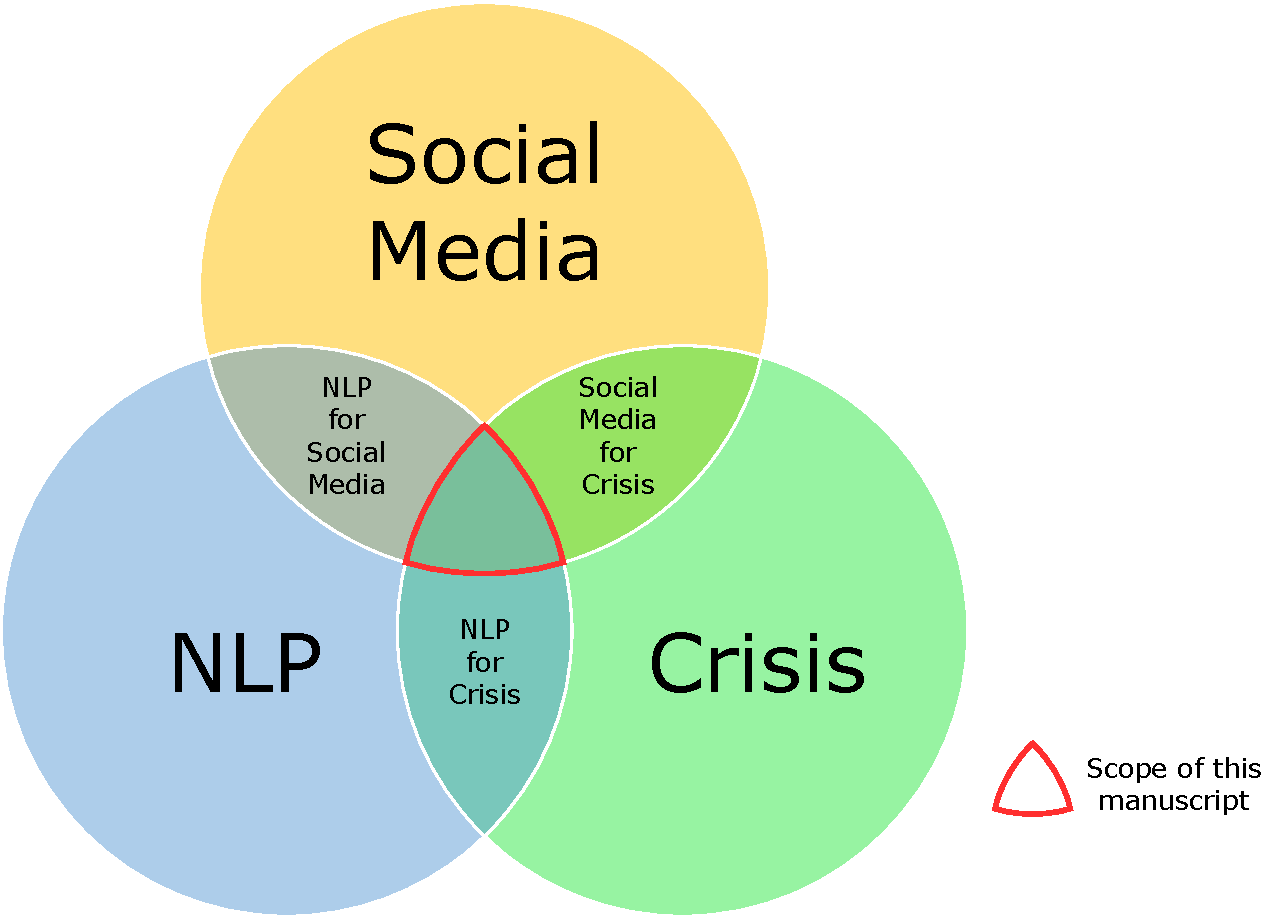
\includegraphics[width=\textwidth]{figures/chap-1/venn-diagram-domains.pdf}
    \caption{Intersection between the domains of Social Media, Crisis Management et Natural Language Processing and the positioning of the research presented in this manuscript.}
    \label{context:venn-diagram-domains}
\end{figure}

\textcite{palenCitizenCommunicationsCrisis2007} highlighted in 2007 the role of information and communication technologies (ICT) in crisis response.
A few years later, social media were considered as an opportunity in crisis management \textcite{viewegMicrobloggingTwoNatural2010}.
This work started the social media branch of crisis informatic \parencite{palenCrisisInformaticsHumancentered2020}.
NLP was then used to automatically retrieve information from the flow of social media data \textcite{vermaNaturalLanguageProcessing2011,carageaClassifyingTextMessages2011}.
This allowed to scale the analysis to the high volume of content that social media have to offer.
Most of the early work was spent in ways to automatically identify crisis related text messages.
Since then, many efforts have been added to explore other opportunities, such as images.
Variations on different types of crises, on NLP techniques, and features used to represent the data were developed and used.
\textcite{imranUsingAISocial2020} identifies several remaining challenges in the domain of social media in crisis informatic:

\begin{itemize}
    \item Crisis event detection
    \item Eyewitness detection
    \item Situational awareness
    \item Actionable information gathering
    \item Damage assessment
    \item Crisis communication
    \item Understanding public reaction
    \item Information veracity
\end{itemize}

All these challenges aim at extracting information from social media media.
They necessarily involve artificial intelligence to identify at scale the mentioned information.
However, as mentioned earlier, social media data are subjectives, fuzzy and prone to rumors.
At the same time, the outcome of NLP models is never 100\% accurate.
Thus, uncertainty is the norm among the information extracted from social media data.
Also, all these information, once created, need to be stored, managed and distributed, to provide
Thus, the following problematic:

\begin{center}
    \fbox{
        \begin{minipage}{0.75\textwidth}
            \centering
            \emph{Main problematic:}

            How to design an information system able to automatically manage and deliver relevant information extracted from social media data?
        \end{minipage}
    }
\end{center}

This main problematic is then decomposed into three sub-problematics.

\subsection{Consecutives challenges to the main problematic}
Three consecutives challenges to the main problematic arise.
Firstly, the objective is to identify

\begin{center}
    \fbox{
        \begin{minipage}{0.75\textwidth}
            \centering
            \emph{Research question 1:}

            What information that can be obtained from social media is relevant to the decisiom makers in crisis response?
        \end{minipage}
    }
\end{center}

Secondly, once relevant information has been identified, one needs to collect the data needed and
extract the information wanted. Thus, the second research question:

\begin{center}
    \fbox{
        \begin{minipage}{0.75\textwidth}
            \centering
            \emph{Research question 2:}

            How can this information be obtained, in the context of crisis informatic?
        \end{minipage}
    }
\end{center}

Thirdly, extracting information is not enough.
This information needs to be managed, to deliver further value, and delivered.
Leading to the third research question:

\begin{center}
    \fbox{
        \begin{minipage}{0.75\textwidth}
            \centering
            \emph{Research question 3:}

            How is this information organised to deliver the value expected by decision makers?
        \end{minipage}
    }
\end{center}

\subsection{The MACIV project}
The MACIV project (Management of Citizens and Volunteers: the social media contribution in crisis situations)
was an opportunity to bring together multiple actors from different institutions around the problematic
of adoption of social media in crisis response.
The objective of the project was to understand the opportunity offered by volunteers in crisis management, especially in the social media space.
This project, funded by the Agence National de la Recherche (ANR), was composed of both
scientific actors — Télécom ParisTech, IMT Mines Albi and —,
institutional actors — Direction Générale de la Sécurité Civile et de la Gestion des Crises, Préfecture de Police de Paris, Service Départemental d'Incendie et de Secours du Var — and
associatives actors — the VISOV (Volontaires Internationaux en Soutien Opérationel Virtuel) association.
This collaboration was illustrated through three different, physical, exercices.

Along this project which took place in France, a significant part of the work presented in this dissertation was fed through a year long in the USA.
This visiting provided opportunities to meet several actors of the American  emergency services that
provided valuable insights that fueled the results presented later in this document.

\section{Structure of the document}
The purpose of this manuscript is to advance the issue of improving situational awareness and collaboration between actors during the response to a crisis event, which was one of the issues identified in the crisis management section.
Thus, adopting the point of view of decision makers, and in the scope of the information system, the main problematic is:

\emph{How to design an information system able to automatically manage and deliver relevant information extracted from social media data?}

The scope and consecutives research questions of this main problematic are illustrated in Figure~\ref{context:big-picture}.

\begin{landscape}
    \begin{figure}
        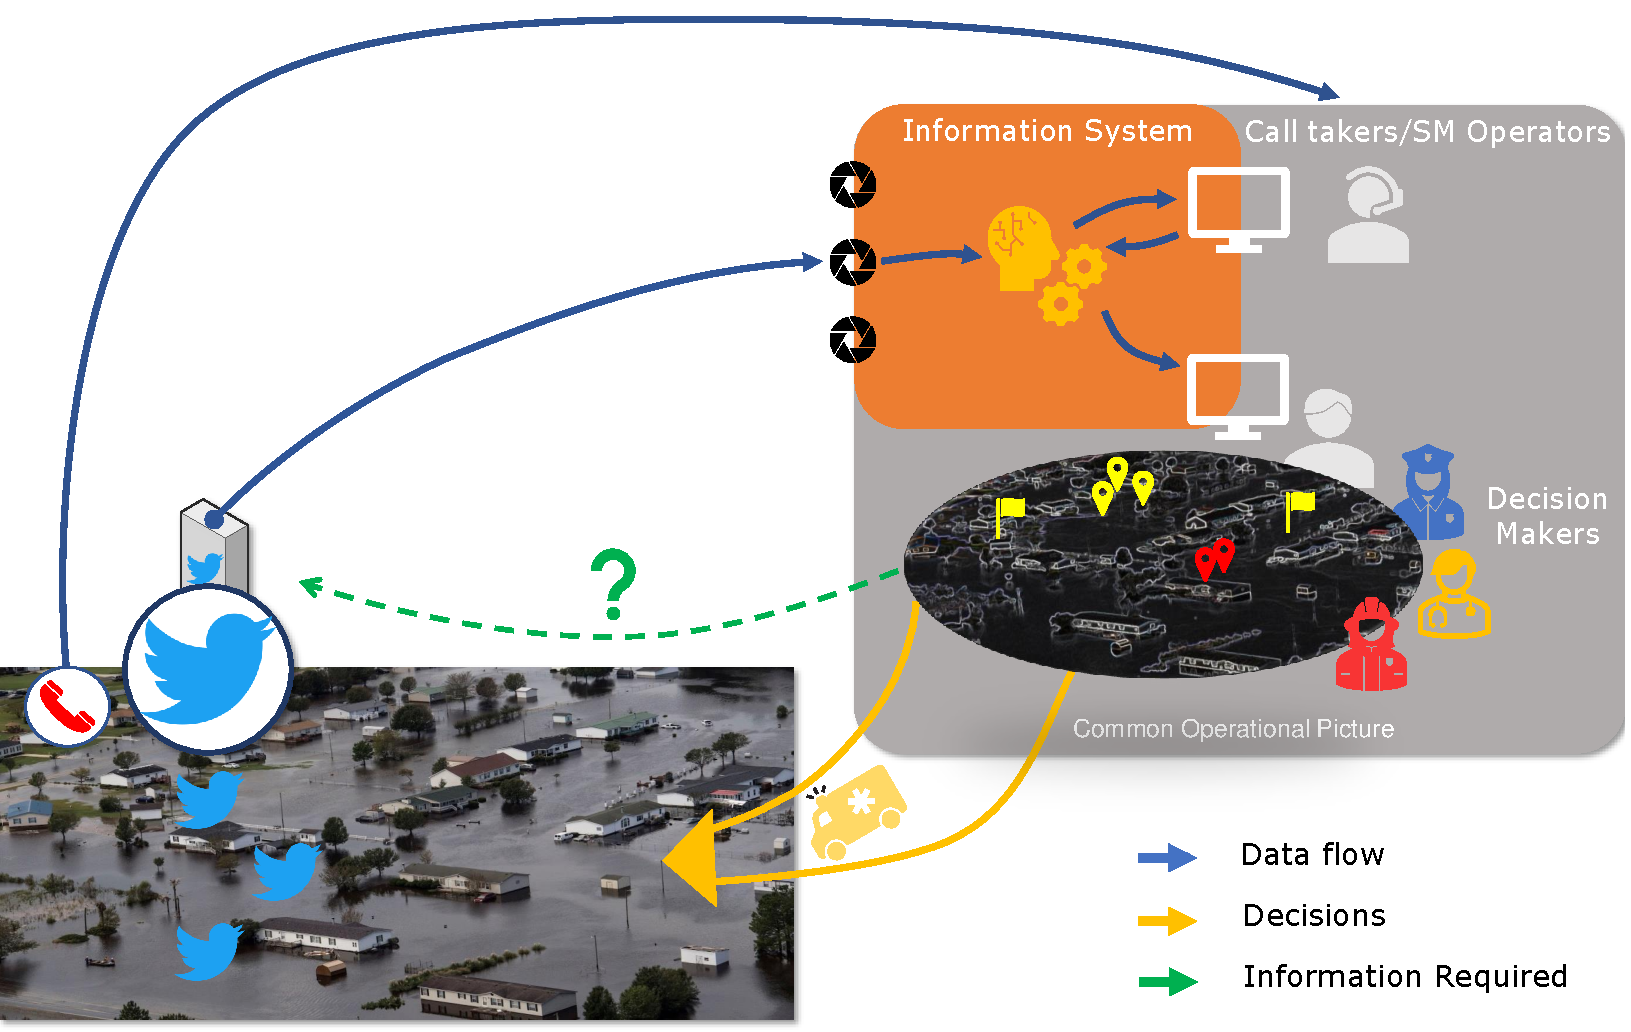
\includegraphics[width=\paperwidth,height=\paperheight,keepaspectratio]{figures/chap-1/big-picture.pdf}
        \caption{Big picture of the manuscript.}
        \label{context:big-picture}
    \end{figure}
\end{landscape}

The next chapter, Chapter 2, is a literature review that explores the scope of each research question.
Chapters 3 to 5 are the contributions associated with each research question.

\begin{itemize}
    \item Chapter 3 narrows the scope of the information system designed by identifying its users and their information needs from an operational point of view.
    \item Chapter 4 describes an algorithm to identify the information needed, while maintaining the user in the information extraction process.
    \item Chapter 5 embeds all the previous contributions in a software architecture for a crisis information system, allowing to structure and build further information.
\end{itemize}

The final chapter, chapter 6, provide conclusion and discussions about this work.

%%% Local Variables:
%%% mode: latex
%%% TeX-master: "../ma-these"
%%% End:


\chapter{Literature review}

\section*{Introduction}
%? Quel est l'objectif de ce chapitre ? Comment se construit-il ?
This chapter presents and discusses previous conducted works related to the three research questions driving this dissertation.
The research questions previously identified are:

\begin{enumerate}
    \item What can decision-relevant information from social media be processed automatically?
    \item How can the actionable information available on social be automatically retrieved during crisis response?
    \item What challenges are faced by an information system dedicated to crisis management that embeds machine learning models?
\end{enumerate}

Each research question has its dedicated section.
Each section presents the evolution of the associated fields and the trends that have guided their development.
The review of this literature allows for the identification of research directions for the following chapters.
The remainder of this section presents the methodology used for the literature review and the research hypotheses.

% TODO Ajouter la collection d'articles de Leysia Palen https://docs.google.com/document/d/1sP6TsuPSCSgoHZKEM7fqZ8BXZccv3JS8TobRJXEHD7Q/edit
\subsection*{Methodology}
A mixed approach was taken to capture the evolution of work related to each research question
First, the scope of the literature review is defined through research hypotheses.
Once these hypotheses are created, the queries are made on Scopus~\footnote{https://www.scopus.com/}, a bibliographic database.

The results obtained are then be analyzed from several angles.
First, the evolution of the volume of publications returned by the query to attempt to represent the interest in the topic.
Secondly, an analysis of the keywords is made through VOSviewer~\footnote{https://www.vosviewer.com/} "a software tool for constructing and visualizing bibliometric networks."
Especially VOSviewer allows visualizing bibliographic features such as the networks of authors or keywords.
The keywords used by the different articles fetched by request provide valuable insights into the evolution of a given field, especially its interdisciplinary aspect.
Finally, the results of the most cited articles are discussed.
This methodology should make it possible to show the evolution of the scientific community's interest in the topics explored.

\subsection*{Hypotheses}
This sub-section establishes the scope of the research conducted in the rest of the chapter.
First, the only data source considered is social media.
As mentioned in the previous chapter, social media data present a set of specificities that differ from other data sources such as newspapers.
Secondly, the literature review is scoped to the crisis management context.
Finally, it is assumed that facilitating decision-making necessarily improves disaster response.
Thus, the following working hypotheses delimit the work presented.

\begin{enumerate}
    \item Social media data: social media data have a low ratio of information/noise.
    \item Crisis management: the crisis management context is particular, and this manuscript focuses on the response phase and its context.
    \item Improving the decision-making process leads to better disaster response.
\end{enumerate}

These hypotheses guide the literature review around the research questions outlined above.
Thus, the first section presents previous works on systems that automatically process social media for crisis response.
Then, the second section explores the first research question and develops on previous representations of information created.
The third and final section overlooks the different attempts to process social media data using Natural Language Processing methods.
As the third research question also refers to systems for processing social media data automatically, it shares the insights of the first section.

\section{Information systems for crisis response fed with social media data}
% * Done
The first chapter identified the opportunities offered by social media to support crisis response.
Many researchers explored these opportunities and proposed various systems and architectures to process social media data automatically.
The ultimate goal of these researches is to provide valuable insights to decision-makers.
This first part of the literature review highlights the main systems built for this purpose.
The research question this part aims to answer is: \emph{What are the existing social media processing system developed for crisis response over the years?}

The request run on the Scopus database is broken down in table~\ref{table:request-information-systems}.
It returns 96 documents published between 2011 and 2021.
The beginning of this domain of research corresponds to the democratization of social media, with the development of social media platforms happening during the 2000-2010 period (Figure~\ref{literature:crisis-informatic-hist}).
Naturally, the field has developed, driven by the need of crisis management organizations and the public interest benefit it promises.

\begin{table}[bht]
    \centering
    \caption{Overview of the bibliographic request related to information systems.}
    \tabulinesep=1.2mm
    \begin{tabu} to \textwidth {X[0.5,r]X[1,m]X[1,m]}
        Type of request & Keywords                                                                                                                                     & Explaination                                                                                                          \\ [0.5ex]
        \toprule
        SUBJAREA        & \textit{comp}                                                                                                                                & Articles in the Computer Science domain                                                                               \\
        TITLE-ABS-KEY   & \textit{crisis management} OR \textit{crisis response} OR \textit{contingency} OR \textit{disaster response} OR \textit{disaster management} & Articles related to crisis management                                                                                 \\
        TITLE-ABS-KEY   & \textit{system} AND \textit{processing}                                                                                                      & And concern systems processing information                                                                            \\
        TITLE-ABS-KEY   & \textit{social media} OR \textit{twitter}                                                                                                    & Using social media sources. Twitter is specifically indicated because of its prevalent use in the research community. \\
        EXCLUDE-DOCTYPE & \textit{re} OR \textit{cr}                                                                                                                   & Reviews and conference tracks introductions are excluded                                                              \\
        \bottomrule
    \end{tabu}
    \label{table:request-information-systems}
\end{table}


\begin{figure}[thb]
    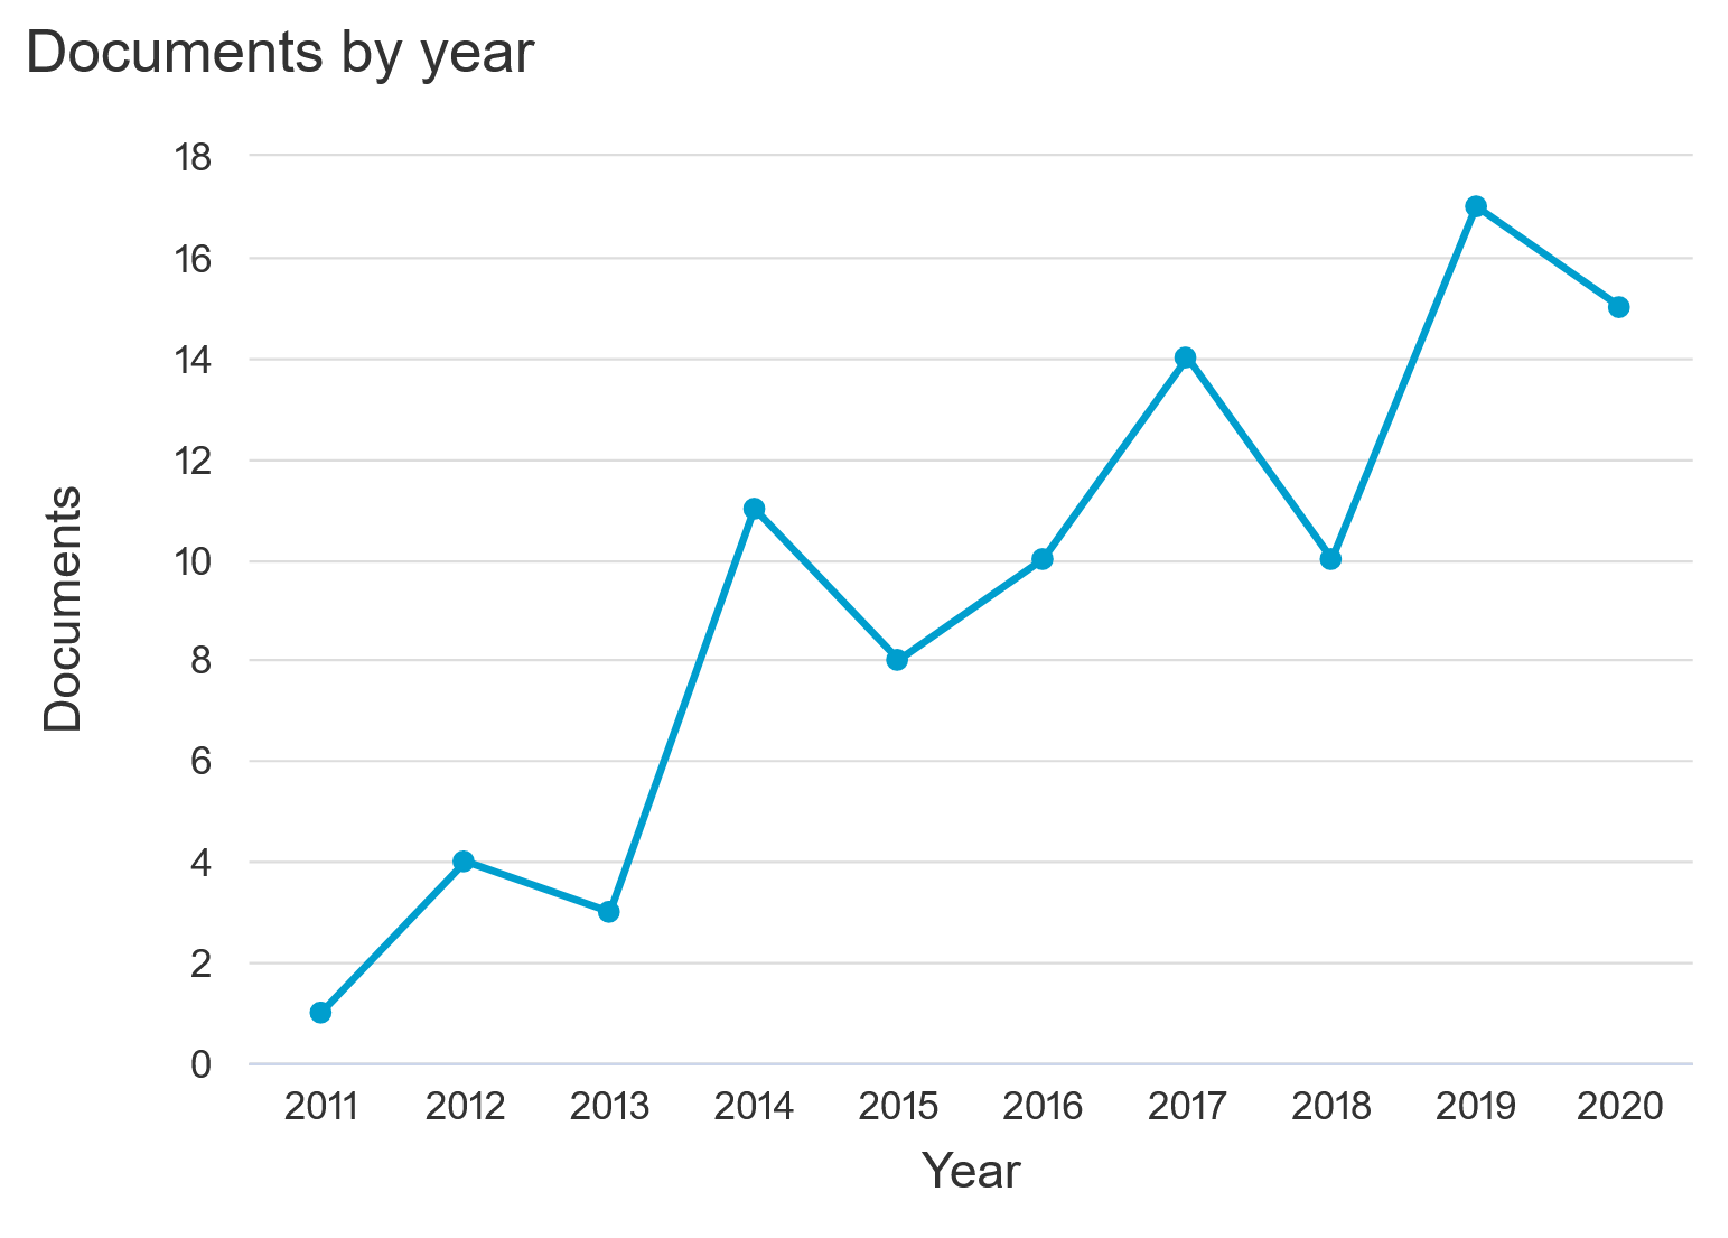
\includegraphics[width=\textwidth]{figures/chap-2/crisis-informatic-hist.pdf}
    \caption{Timeline of the volume of contributions per years for the crisis informatic domain. The year 2021 is excluded because the year is not complete at the time of writing.}
    \label{literature:crisis-informatic-hist}
\end{figure}

The network provided by VOSviewer (Figure~\ref{literature:crisis-informatic-overlay}) does not reveal any significant cluster of keywords.
The youth of the domain can explain the structure observed, as no prominent direction as been created yet.
However, the publication timeline (represented by the color variation) provides insights into the direction of the domain.
Years around 2016 mainly were focused on data analyses of the different datasets available.
Then, the following years saw the development of more and more automation.
Artificial intelligence, machine learning, and natural language processing appeared in that chronological order, coinciding with the progress made in these areas.
More recently, deep learning models to process text and images are appearing, as well as new opportunities created by the internet of things and the development of the concept of smart cities.
It is also worth noting that social and computer sciences are blended in this big picture.

\begin{landscape}
    \begin{figure}[hp]
        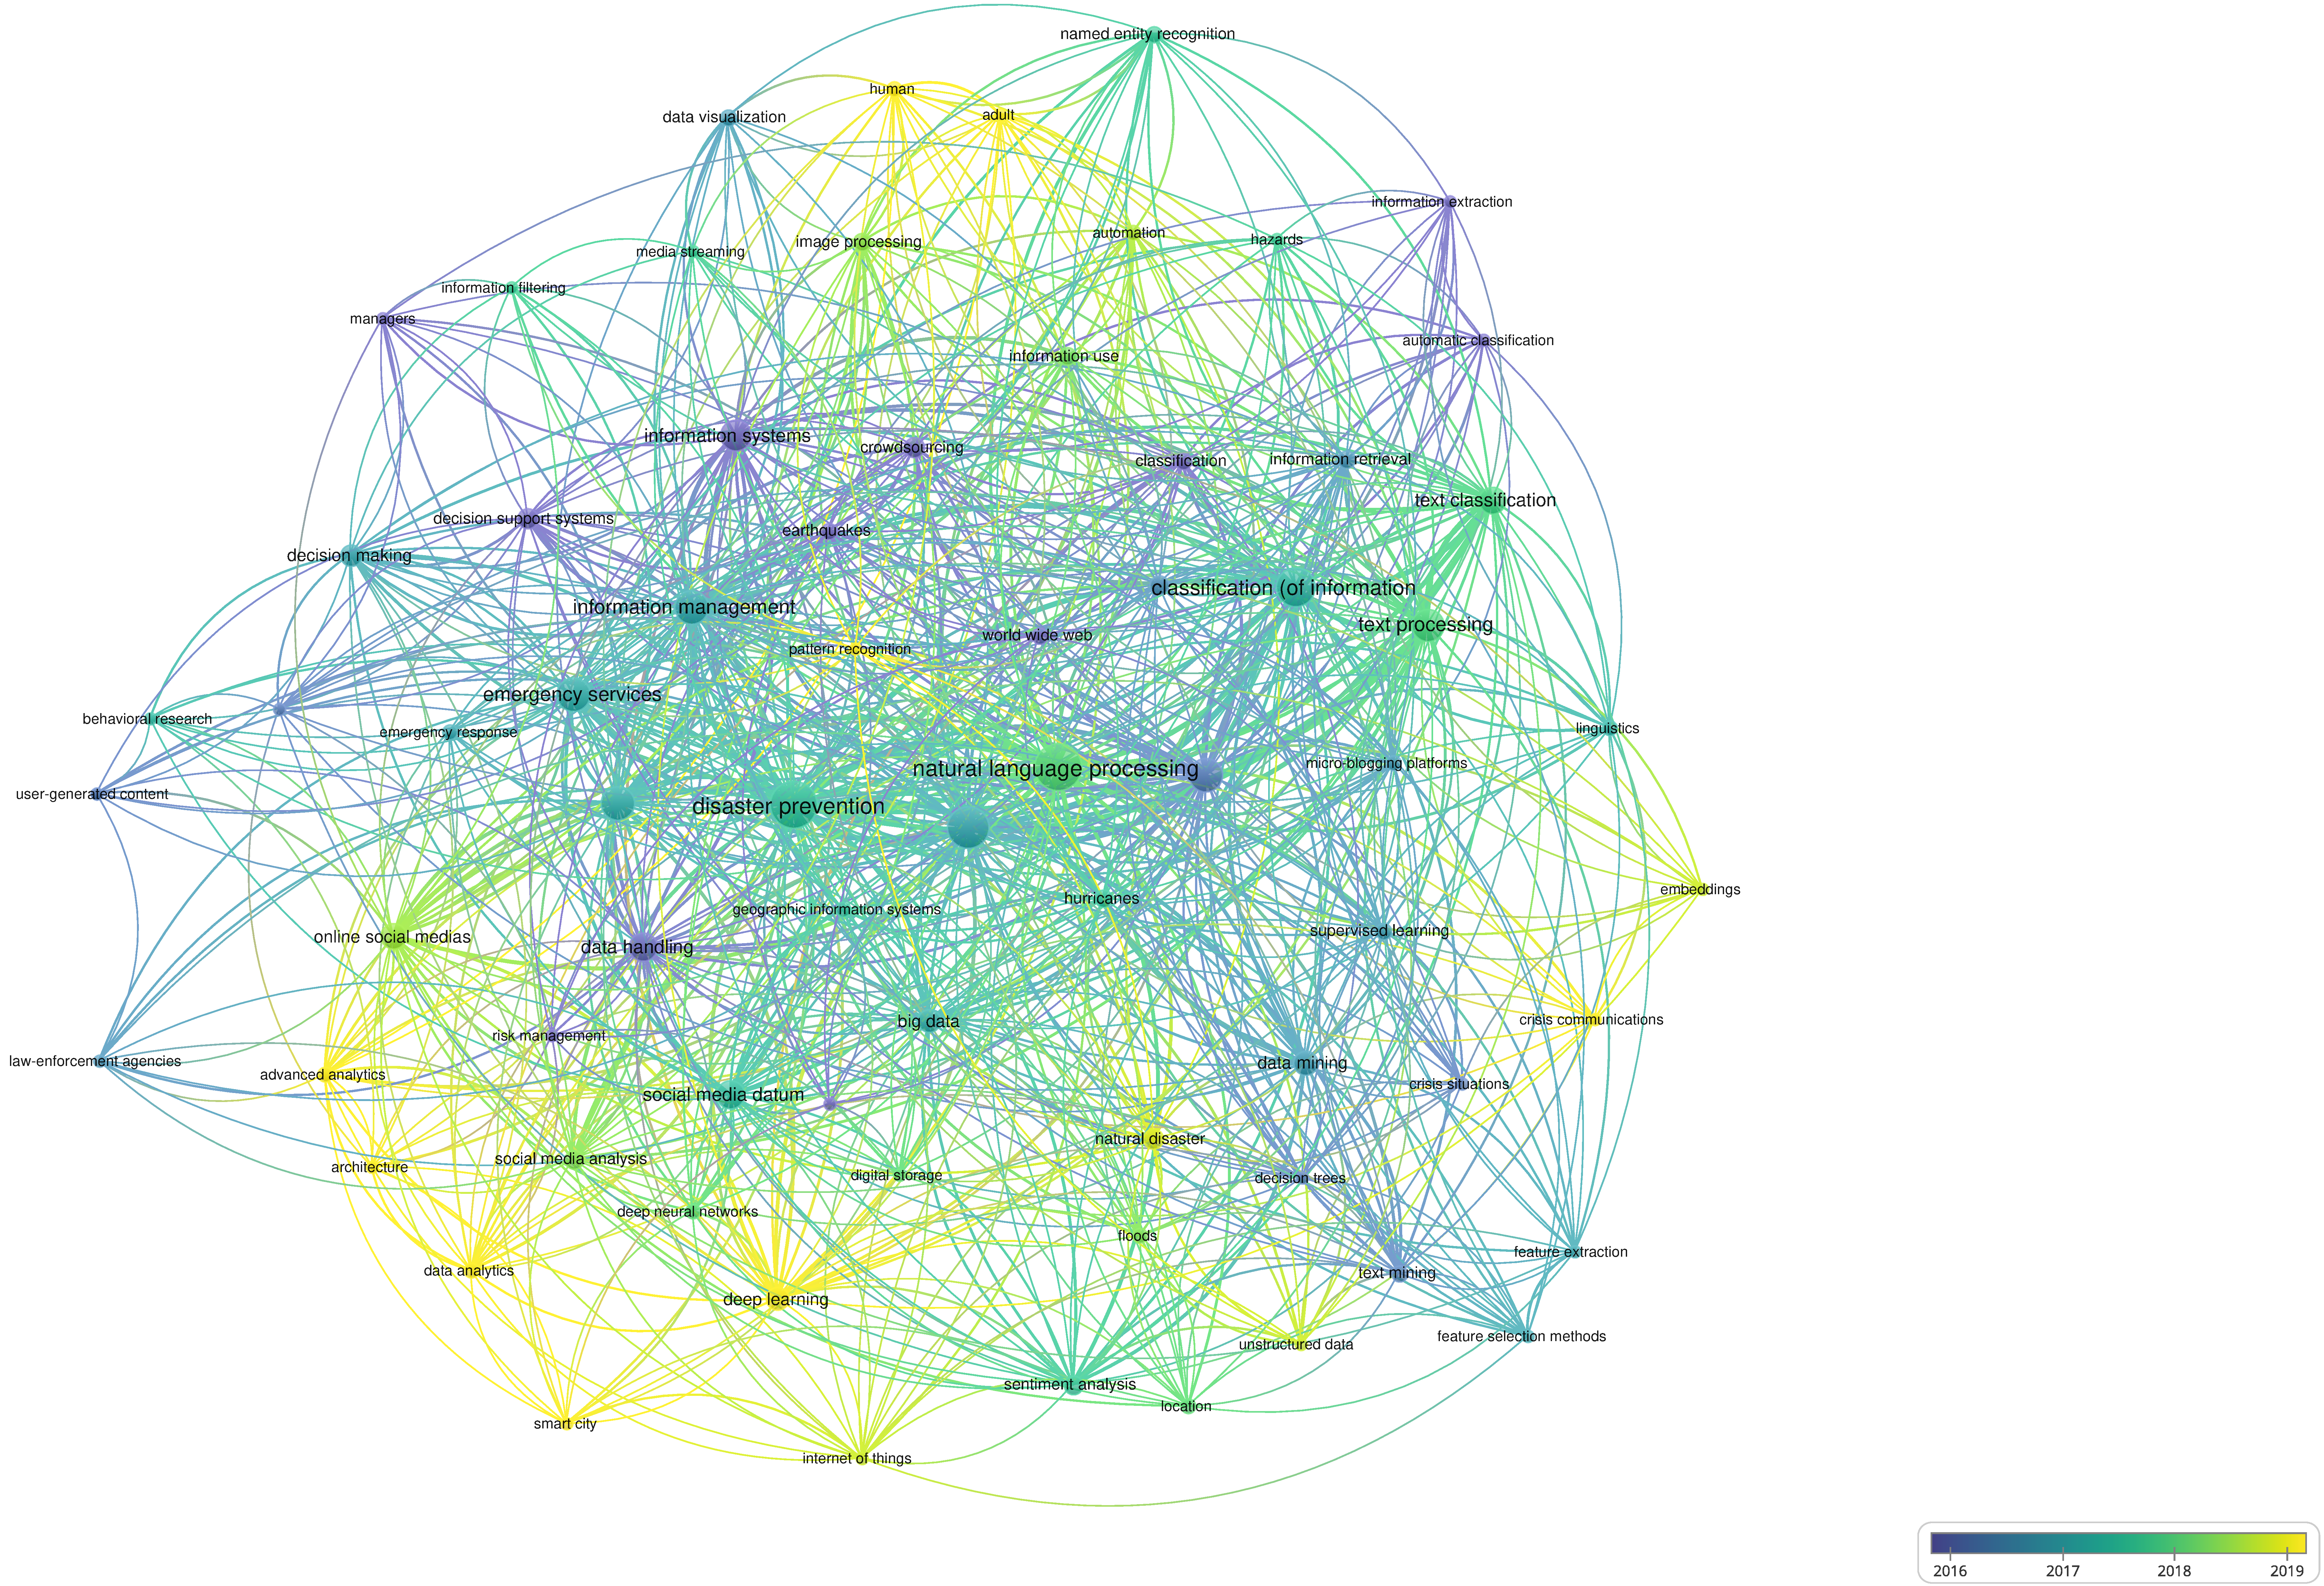
\includegraphics[width=\paperwidth,height=\paperheight,keepaspectratio]{figures/chap-2/crisis-informatic-overlay.pdf}
        \caption{Distribution of keywords with more than 3 occurrences among the articles from the query on crisis informatics. }
        \label{literature:crisis-informatic-overlay}
    \end{figure}
\end{landscape}

The bar diagram (Figure~\ref{literature:crisis-informatic-bar}) provides a representation of the distribution of the occurrences of the different keywords.
From the most used keywords, two areas of interest seem to emerge.
The first one is the automatic processing of social media data.
The type of data appears to be primarily textual, according to the prevalent use of \emph{natural language processing} and \emph{text processing} is no more important than the use of this automation.
\emph{Disaster prevention}, \emph{situation awareness}, \emph{information management} and \emph{emergency services} highlight the importance of the applications of the results.

\begin{figure}[thb]
    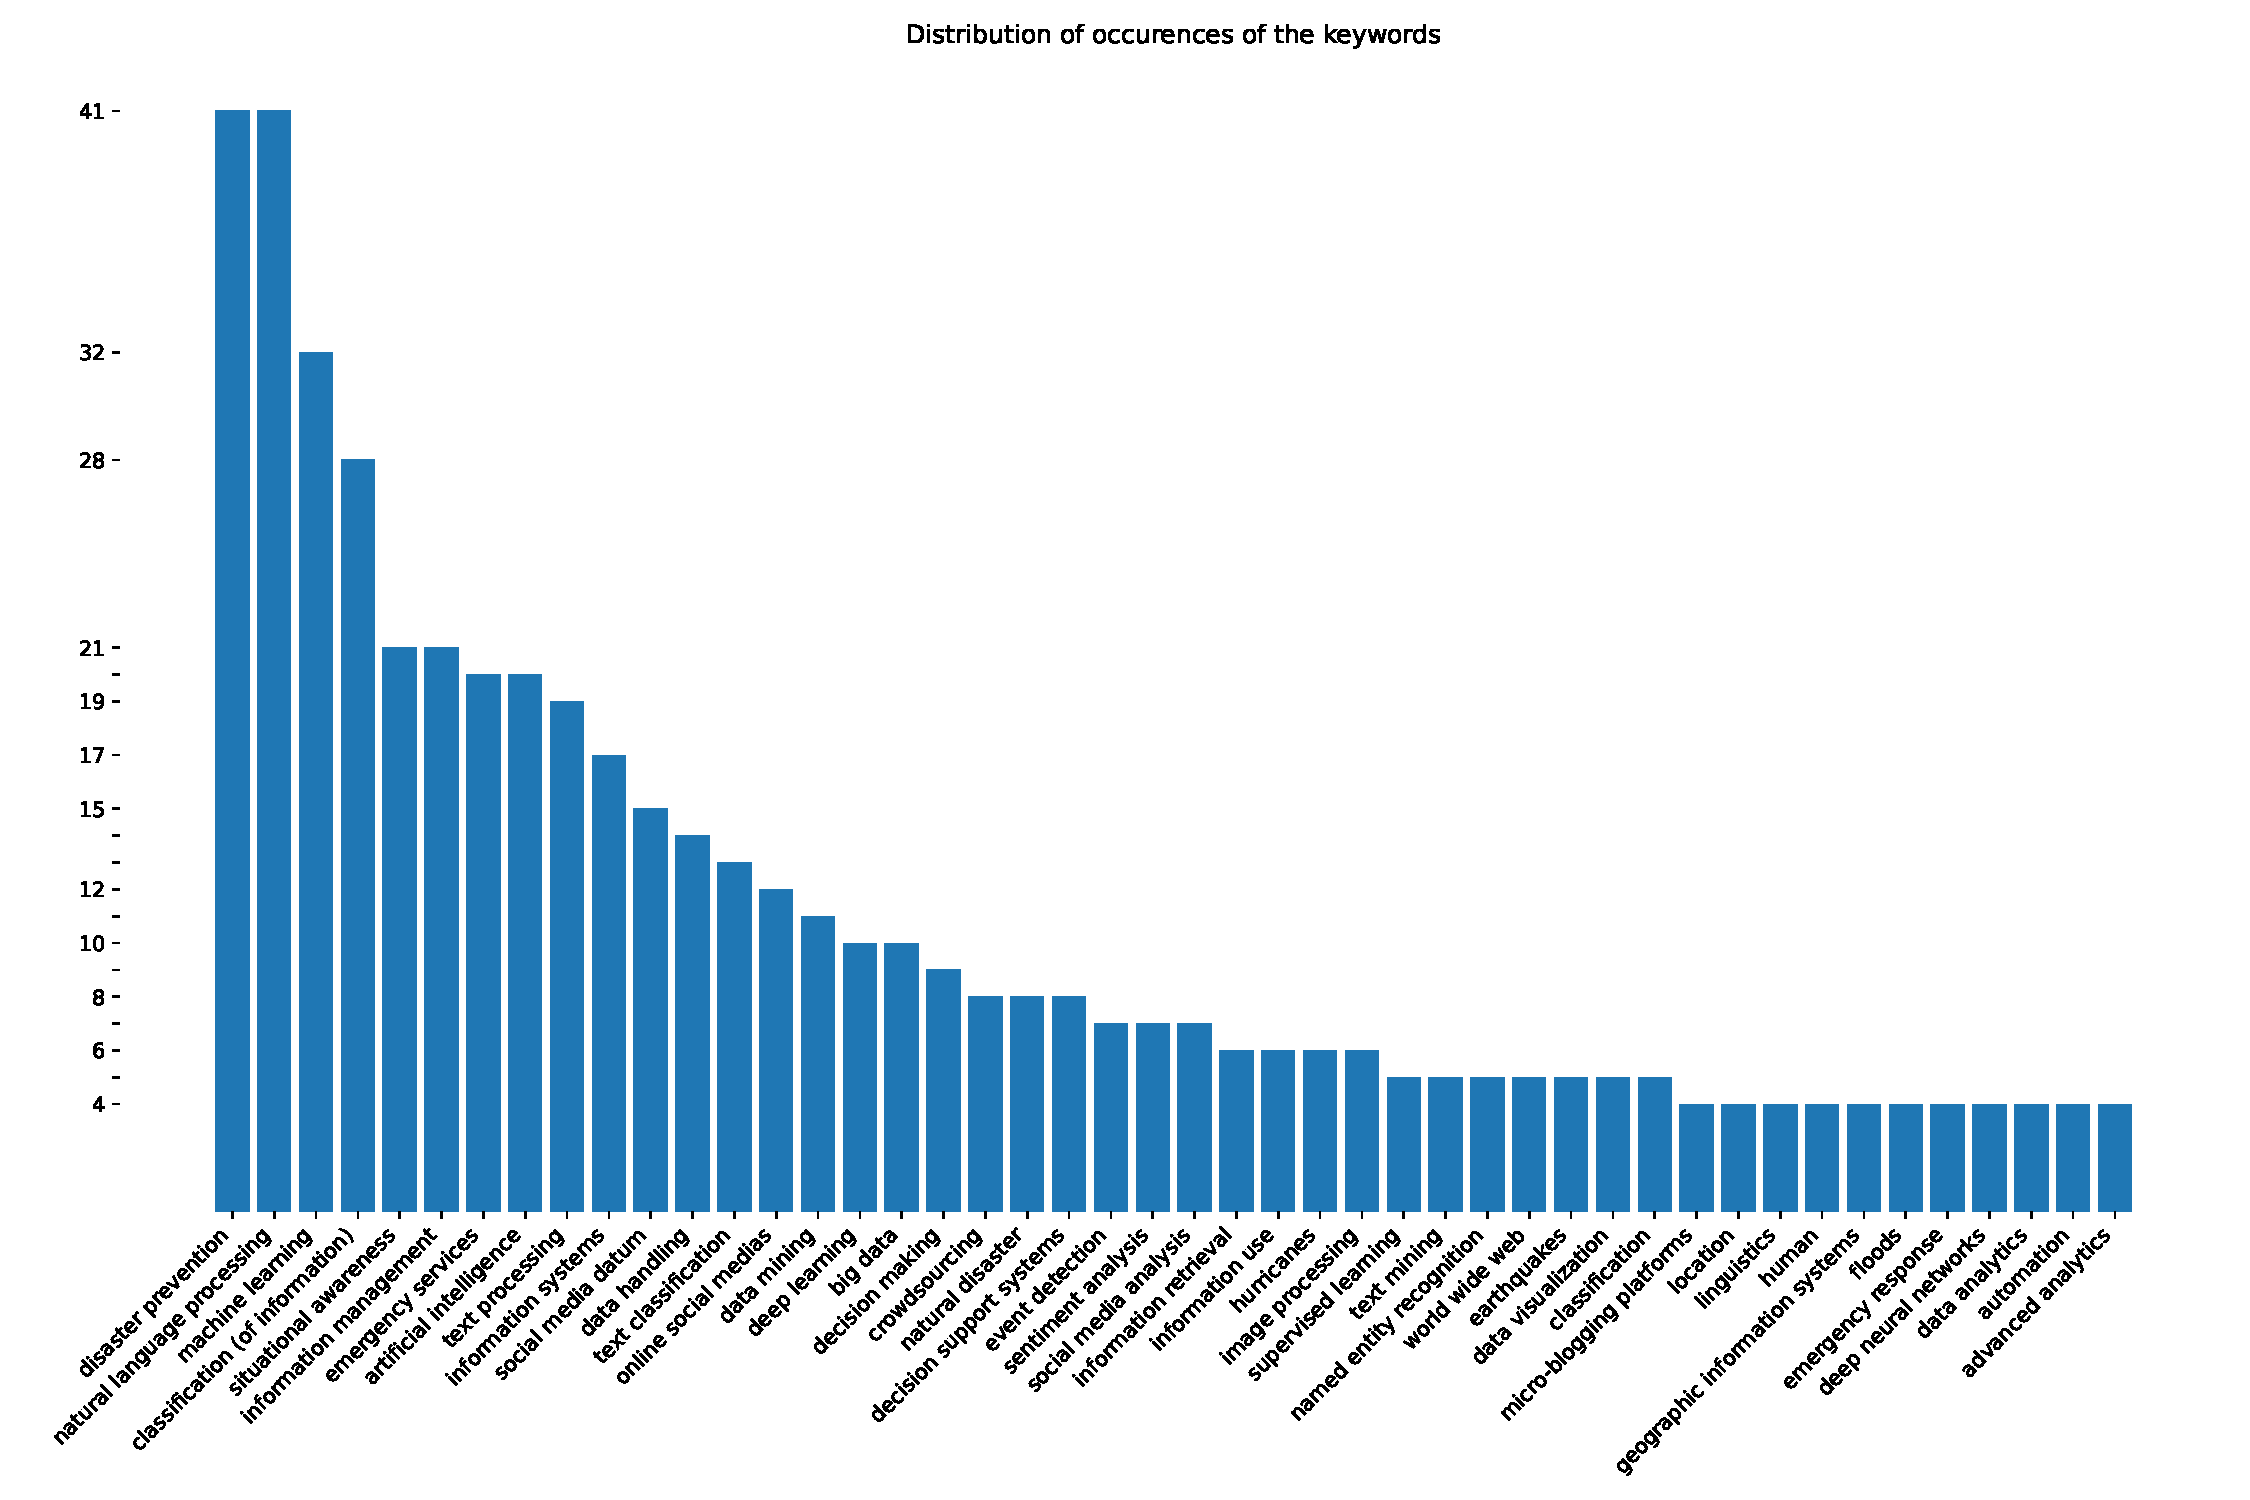
\includegraphics[width=\textwidth]{figures/chap-2/crisis-informatic-bar.pdf}
    \caption{Distribution of keywords with more than 3 occurrences among the articles from the query on crisis informatics. }
    \label{literature:crisis-informatic-bar}
\end{figure}

As mentioned in the first chapter, automatically processing the content of social media to extract information is a new and promising scientific venue.
Thus, many attempted to create systems to achieve this goal, proposing features to improve usability.
Table~\ref{table:crisis-informatic-main-articles} presents the results of the previous query that mention a processing system that uses social media as a data source and that has been cited at least ten times are shown.
The right column of the table summarizes the main features proposed by the authors.

Among the features identified, the trend towards automation observed earlier is clear.
The first iterated systems were mainly relying on crowdsourcing to identify relevant information from messages posted on social media
\parencite{schulzCrisisInformationManagement2012, backfriedOpenSourceIntelligence2012,imranAIDRArtificialIntelligence2014}.
The following works were interested in automating the previous tasks to reduce the dependence on human resources and improve massive data processing.
Problems related to the detection of occurence of events and their related information on social media, have been explored using different approaches \parencite{imranAIDRArtificialIntelligence2014,middletonRealtimeCrisisMapping2014,avvenutiEARSEarthquakeAlert2014, gibsonCombiningBigSocial2014}.
In parallel, experiments were conducted to identify the best ways to organize and disseminate the information obtained \parencite{middletonRealtimeCrisisMapping2014,huangDisasterMapperCyberGISFramework2015,avvenutiPullingInformationSocial2016,grunder-fahrerTopicsTopicalPhases2018}.
Building on its successes, the field has continued to develop by relying on other available data formats and in particular images \parencite{alamImage4ActOnlineSocial2017,nguyenAutomaticImageFiltering2017,agarwalCrisisDIASMultimodalDamage2020}.
Beyond the data, new questions have emerged, following feedback from the emergency departments involved in the experiments.
The detection of sub-events and the different concerns of the impacted population is added to the results of previous works \parencite{wuStreamExplorerMultiStageSystem2018,raginiBigDataAnalytics2018,grunder-fahrerTopicsTopicalPhases2018}.
More recently, teams with a broader vision are interested in the integration of such systems within smart cities \parencite{shahDisasterResilientSmart2019}.
The multiplication of sources and formats naturally leads to the need for unified processing methods for data and fusion of information obtained by the different channels \parencite{alamDescriptiveVisualSummaries2020}.

This introductory section presented previous works around crisis informatics.
More particularly, it highlighted the development of the field over time.
This development is directly reflected in the different systems developed and their features.
An interesting trend to note is the move towards more and more automation in systems.
First, using crowdsourcing for initial data labeling, the following systems used machine learning to classify the data into different categories.
Currently, automation was further extended to other valuable data types and ways to merge the information acquired.

\begin{table}[bh]
    \centering
    \tabulinesep=1.2mm
    \caption{Articles retrieved from the previous request which propose social media processing systems or methods with at least 10 citations.}
    \begin{tabu} to \textwidth {X[3,m]X[1.5,m]X[5,m]}
        Reference                                       & Type of event studied & Features                                                 \\ [0.5ex]
        \toprule
        \cite{schulzCrisisInformationManagement2012}    & None                  & Crowdsourcing                                            \\
        \cite{backfriedOpenSourceIntelligence2012}      & None                  & Crowdsourcing, Automatic processing                      \\
        \cite{imranAIDRArtificialIntelligence2014}      & None                  & Crowdsourcing, Information categories, Message filtering \\
        \cite{middletonRealtimeCrisisMapping2014}       & None                  & Common Operational Picture, Location inference           \\
        \cite{avvenutiEARSEarthquakeAlert2014}          & Earthquake            & Event detection                                          \\
        \cite{gibsonCombiningBigSocial2014}             & None                  & Formal concept analysis, Rule-based method               \\
        \cite{glasgowOurGriefUnspeakable2014}           & None                  & Death-related content detection                          \\
        \cite{huangDisasterMapperCyberGISFramework2015} & None                  & Big Data, Common Operational Picture                     \\
        \cite{avvenutiPullingInformationSocial2016}     & Earthquake, Flooding  & Event detection, Message filtering, Disaster management  \\
        \cite{alamImage4ActOnlineSocial2017}            & None                  & Image processing, Infrastructure damage                  \\
        \cite{fersiniEarthquakeManagementDecision2017}  & Earthquake            & Message filtering, Information management                \\
        \cite{nguyenAutomaticImageFiltering2017}        & None                  & Image processing, De-duplication, Image filtering        \\
        \cite{raginiBigDataAnalytics2018}               & Flooding              & Sentiment analysis                                       \\
        \cite{shahDisasterResilientSmart2019}           & Earthquake, Tsunami   & Smart Cities, IoT integration                            \\
        \cite{grunder-fahrerTopicsTopicalPhases2018}    & None                  & Topic modeling, Disaster management                      \\
        \cite{wuStreamExplorerMultiStageSystem2018}     & None                  & Subevent detection, Clustering                           \\
        \cite{agarwalCrisisDIASMultimodalDamage2020}    & None                  & Damage identification, Severity detection                \\
        \cite{alamDescriptiveVisualSummaries2020}       & Hurricane             & Information fusion                                       \\
        \bottomrule
    \end{tabu}
    \label{table:crisis-informatic-main-articles}
\end{table}

\section{Decision-making in crisis situation}
This part of the literature review explores the bibliographic context around the first research question: \emph{What can decision-relevant information from social media be processed automatically?}
Decision-making is at the heart of the response during a disaster.
Ideally, the right decisions need to be made at the right time.
This expectation is theoretical.
This section is split into three parts.
The first part presents the previous attempts to represent the context of crisis management.
The second part highlights the challenges faced by decision-makers when responding to disasters.
The third and final part refines the previous findings on those which consider social media.

\subsection{Organization of information during crises: crisis models}
\label{sec:lit-information-models}
With the advent of computers to delegate tasks, many have thought of charging some parts of crisis management to machines.
However, in order to delegate these tasks to computers, they must first be provided with a representation of these tasks.
In the context of crisis management, these are representations of the environment of this management.
These representations will be called crisis models in this dissertation.
Two paths to represent crisis' concepts have been taken: ontologies and metamodels.
Ontologies and metamodels have very close definitions.
Both methods aim at creating a controlled vocabulary to define the entities and their relations in a given domain.
These two methods differ in what they seek to produce \parencite{assmannOntologiesMetamodelsModeldriven2006}.
On the one hand, ontologies \emph{define} concepts, providing a vocabulary and a grammar for manipulating the concepts studied.
On the other hand, metamodels \emph{represent} computationally the studied concepts, preferably using a standard modeling language.
More precisely, they seek to represent the information associated with the concept.
Therefore, metamodels and information models will both be used interchangeably in the following.
Standard modeling languages such as the Unified Modeling Language (UML) are preferred as they ease the distribution and development of these representations.
As the backbone of model-driven engineering, Metamodels tend to be developed with interoperability between different systems in mind.
Ontologies and metamodels have been both applied to crisis management.
Due to the tremendous variety induced by crises themselves, many ontologies and metamodels have been proposed to represent different aspects of crisis management.
Consequently, ontologies and information models emerged to represent the informational concepts manipulated during an emergency.
This sub-section aims at retrieving from the literature the different key informational concepts useful for decision-makers during crisis response.
The query used to explore this domain is summarized in Table~\ref{table:crisis-models}.

\begin{table}[bht]
    \centering
    \tabulinesep=1.2mm
    \caption{Overview of the bibliographic request related to crisis models.}
    \begin{tabu} to \textwidth {X[0.5,r]X[1,m]X[1,m]}
        Type of request & Keywords                                                                                                                                     & Explaination                                             \\ [0.5ex]
        \toprule
        SUBJAREA        & \textit{comp}                                                                                                                                & Articles in the Computer Science domain                  \\
        TITLE-ABS-KEY   & \textit{crisis management} OR \textit{crisis response} OR \textit{disaster management} OR \textit{contingency} OR \textit{disaster response} & Articles related to crisis management                    \\
        TITLE-ABS-KEY   & \textit{ontology} OR \textit{metamodel}                                                                                                      & And methods to represent and model information           \\
        EXCLUDE-DOCTYPE & \textit{re} OR \textit{cr}                                                                                                                   & Reviews and conference tracks introductions are excluded \\
        \bottomrule
    \end{tabu}
    \label{table:crisis-models}
\end{table}

The request returns 205 documents published between 1998 and 2021.
Figure~\ref{literature:situation-models-hist} shows the evolution of the volume of publication during this period.
According to the Scopus database, the field has emerged around 2000 and progressed over ten years to reach a plateau of fifteen articles on average per year.
The objective of this research was to identify and organize the information and knowledge used in crisis management.
As mentioned before, the final goal is to delegate part of the management of this information to computers.
For this, it is necessary to structure the required information and knowledge.

\begin{figure}[thb]
    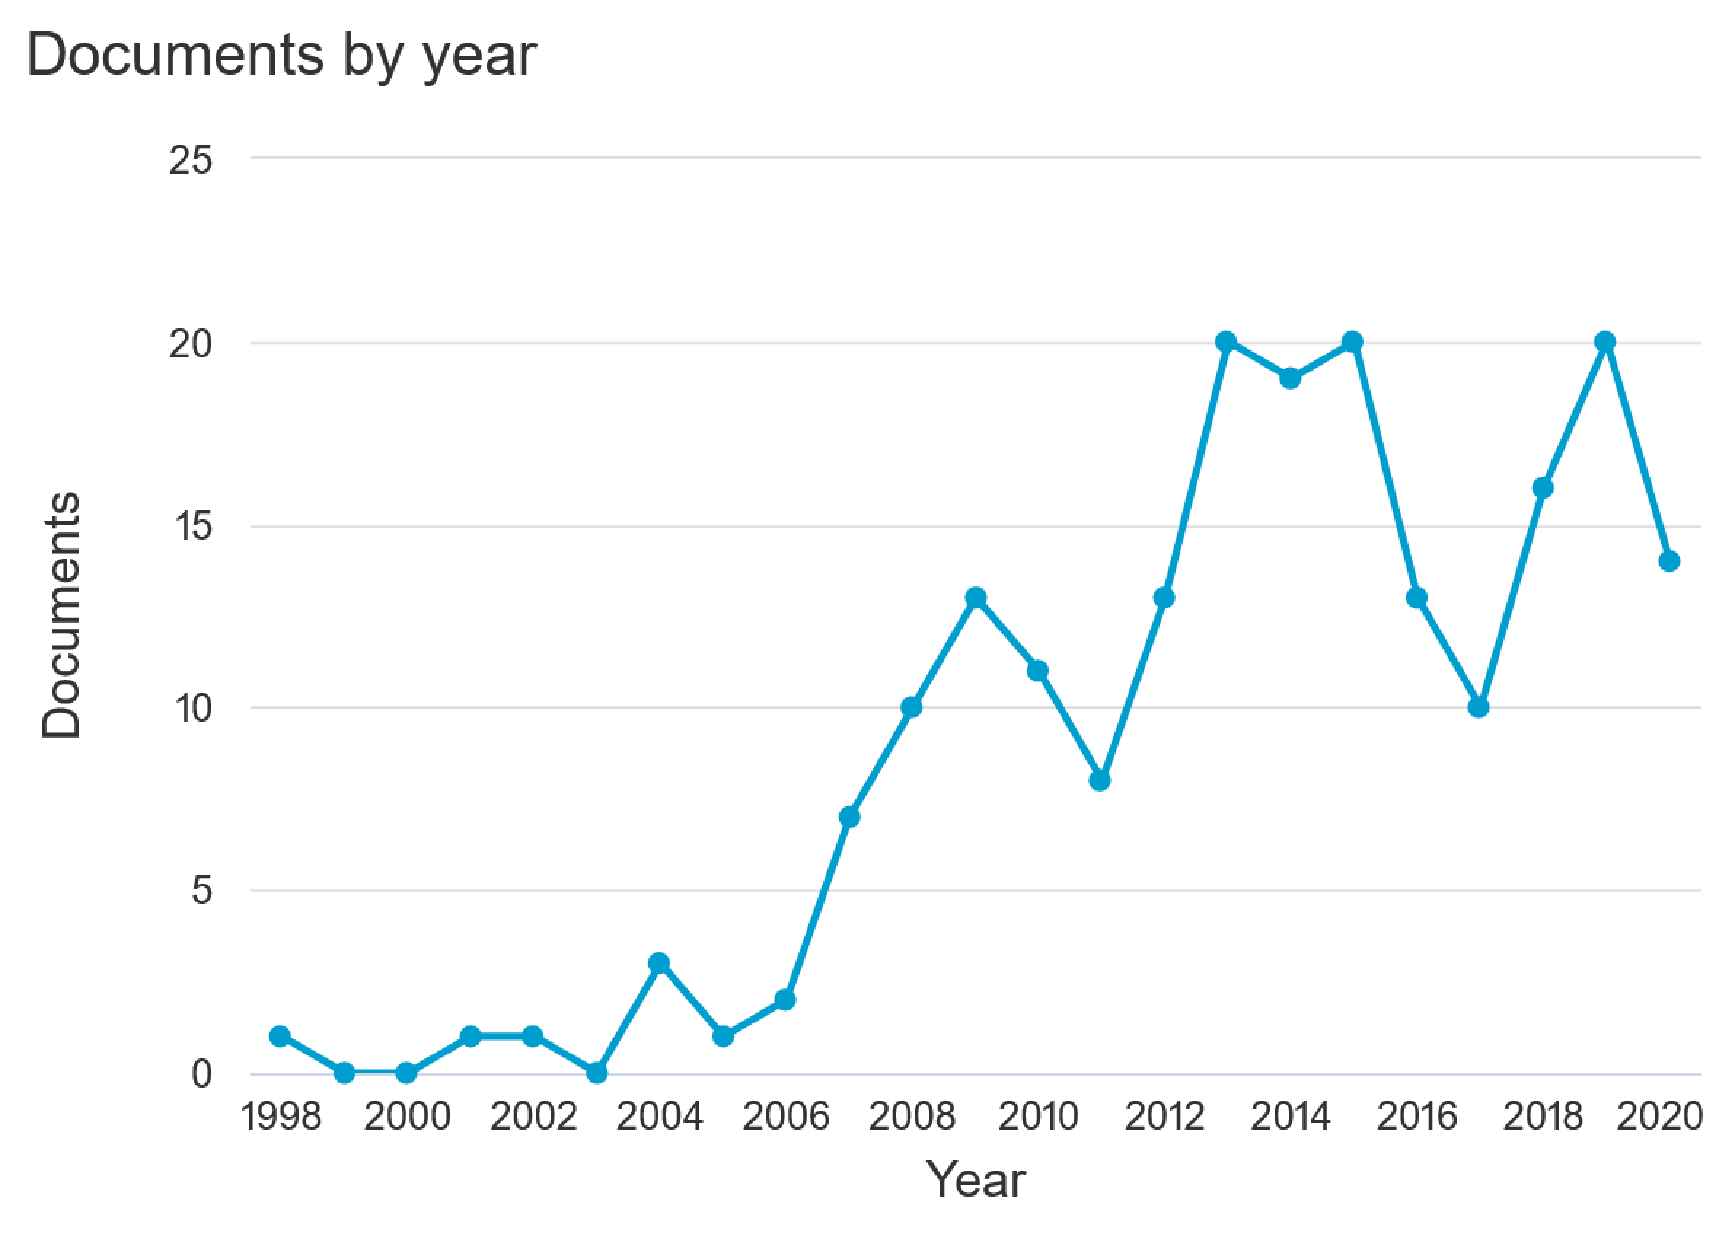
\includegraphics[width=\textwidth]{figures/chap-2/situation-models-hist.pdf}
    \caption{Timeline of the volume of contributions per years for the crisis-situation models domain. The year 2021 is excluded because the year is not complete at the time of writing.}
    \label{literature:situation-models-hist}
\end{figure}

Following the same methodology as in the previous section, Figure~\ref{literature:situation-models-overlay} provides a visual of the evolution over time of the different keywords used in the fetched articles.
The overlay indicates three clusters: a major one and two smaller ones.
The primary cluster focuses on the literature review topic, while the two smaller ones mainly refer to outlier topics (the petroleum and medical sectors).
As in the previous section, the evolution (represented by the color variation) of the keywords hints at the direction of the domain over time.

\begin{landscape}
    \begin{figure}[hp]
        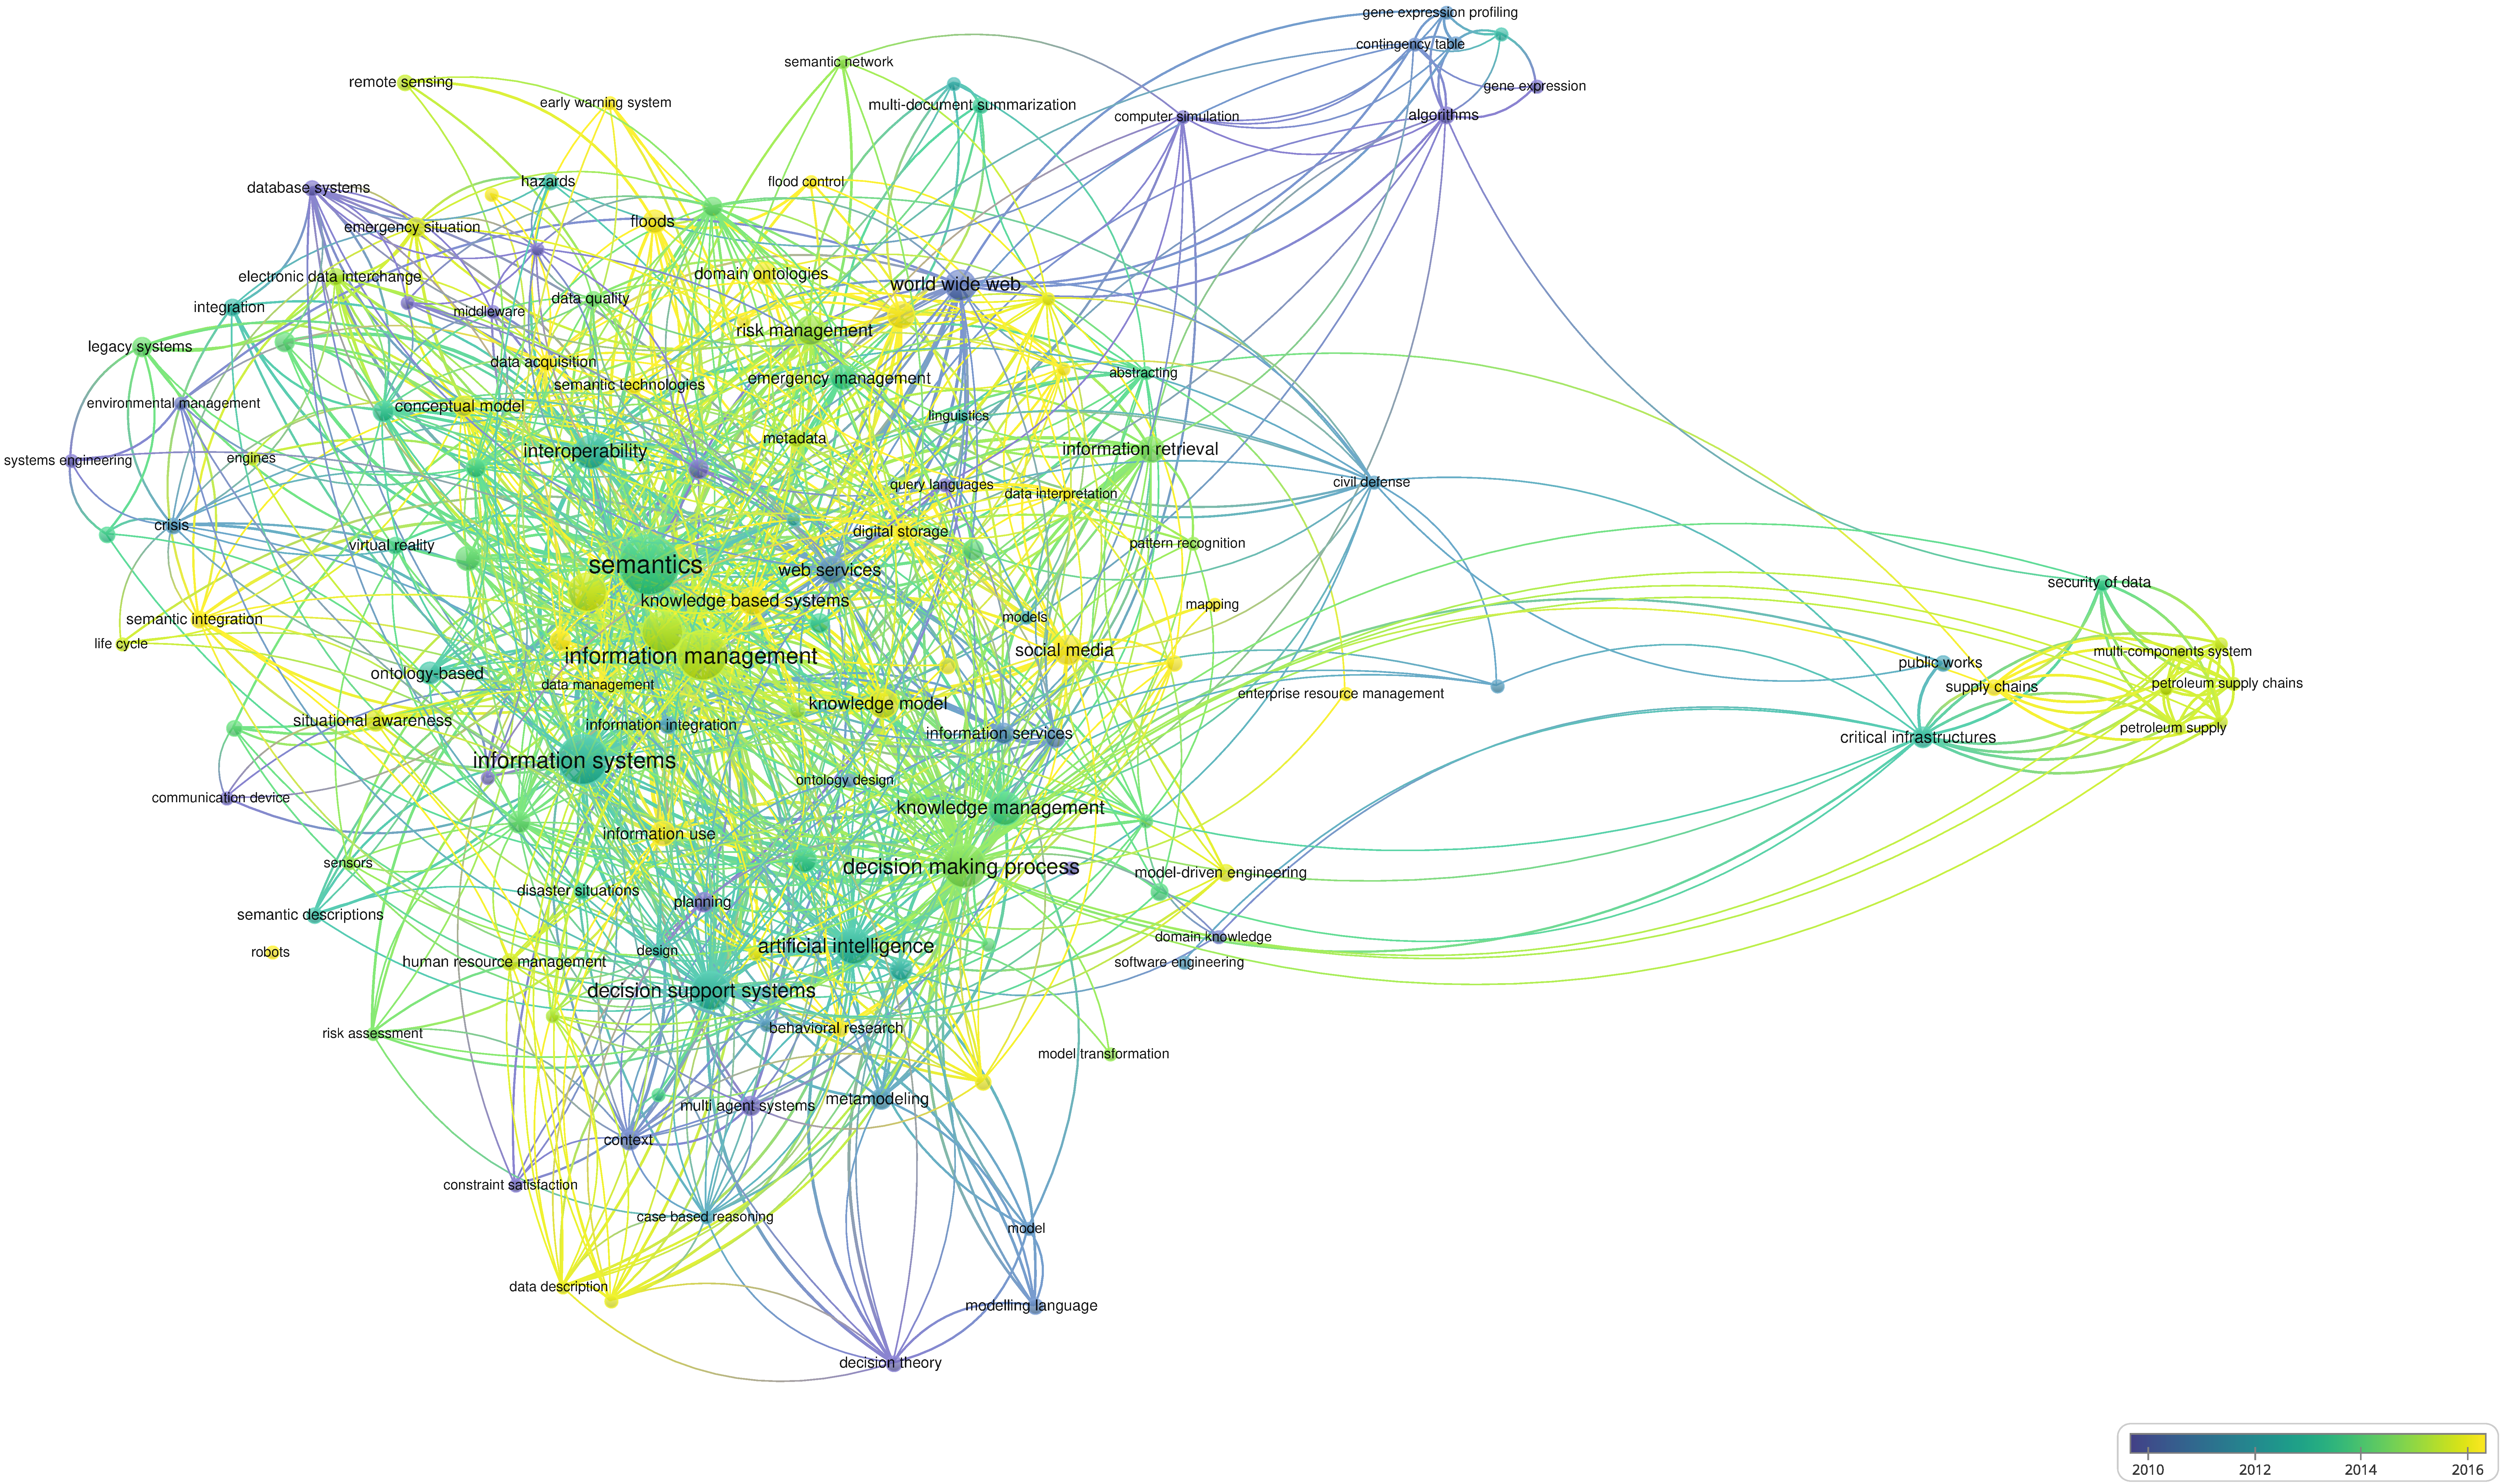
\includegraphics[width=\paperwidth,height=\paperheight,keepaspectratio]{figures/chap-2/situation-models-overlay.pdf}
        \caption{Distribution of keywords with more than 3 occurrences among the articles from the query on crisis-situation models.}
        \label{literature:situation-models-overlay}
    \end{figure}
\end{landscape}

The overlay spans from 2010 to 2016, as it filters keywords with less than three occurrences.
By cross-checking this information with the previous histogram, one understands the reason for this short period.
The histogram shows a low number of publications between 1998 and 2006, while the overlay shows an important variety of keywords used.
This pattern reflects the novelty of the domain.
The stop of the overlay in 2016 can be explained by the loss of interest in this topic from 2015.
Also, according to the histogram, the field regained interest in 2017, indicating that it is on a plateau overall.

Despite this short covered span, it is possible to identify keywords use trends similar to those in crisis informatics.
The older keywords used, such as \emph{SOA}, \emph{simulation}, \emph{multi-agent systems}, and \emph{systems engineering}, show an interest centered around the core of what we're used ontologies and metamodels for—model-driven engineering and information management.
Then, the field knew a pic of interest, as the previous histogram showed.
This period reflects on Figure~\ref{literature:situation-models-bar}, where one can observe that most of the most important keywords are located between 2012 and 2014.
As explained previously, the years between 2012 and 2014 were the most prolific.
These years were primarily focused on the idea of crisis management systems powered by artificial intelligence for decision support.
Artificial intelligence would automatically create the information representations needed by systems.
As these representations would have been written in a standard way, these systems would have adapted to new models, providing greater interoperability quickly.
After this period, the interest in the field decreases a few before coming back with new approaches.
Knowledge-based systems and knowledge management started to appear and a reborn of metamodel and ontologies creation, powered by improvements in machine learning.

\begin{figure}[thb]
    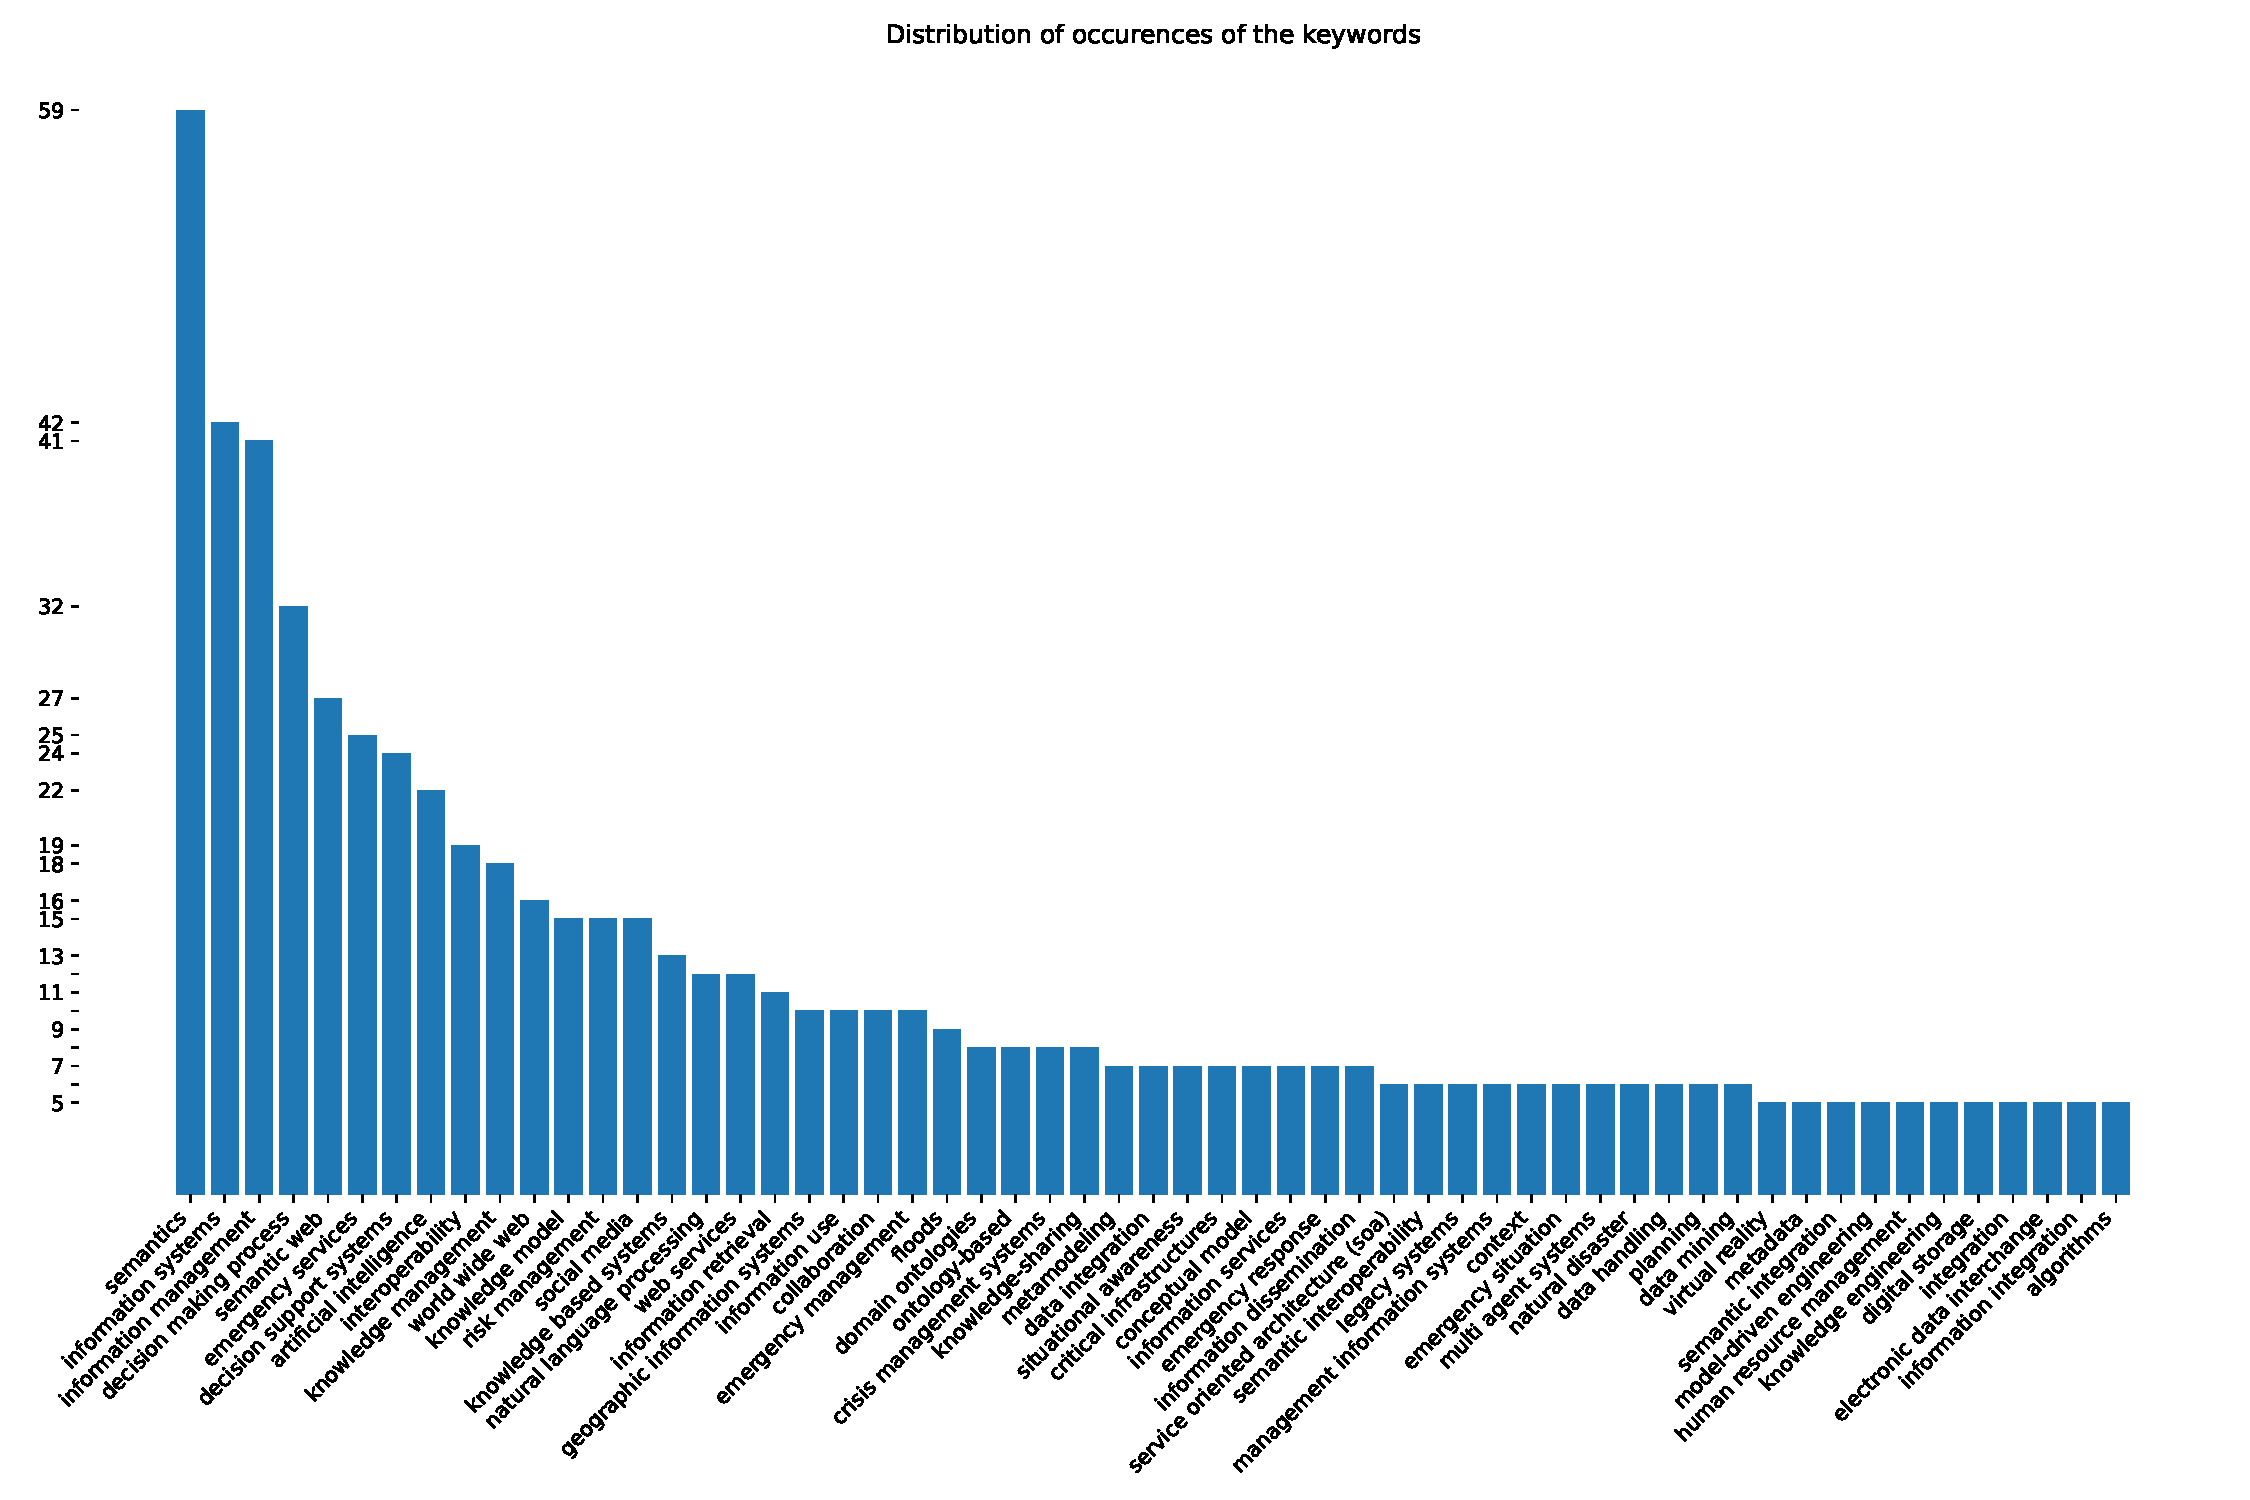
\includegraphics[width=\textwidth]{figures/chap-2/situation-models-bar.pdf}
    \caption{Distribution of keywords with more than 4 occurrences among the articles from the query on crisis-situation models.}
    \label{literature:situation-models-bar}
\end{figure}

In association with the previous qualitative review of the field, Table~\ref{table:situation-models-main-articles} presents the needs of the decision-maker identified in the articles from the previous request with at least 25 citations.
Duplicates and unrelated articles (e.g., gene ontologies) are also excluded.
This review of the main articles highlights the diversity of approaches covered by ontologies and metamodels.
Some of these ontologies are specific to certain events \parencite{xuModelingRepresentationEarthquake2014,qiuIntegratedFloodManagement2017,jungOntologydrivenSlopeModeling2015}.
While these models effectively deal with the type of disaster they are designed for, most of their concept representations do not fit with other types of events.

As mentioned in the first chapter, a proper collaboration between crisis management actors is crucial for disaster response.
Thus \textcite{benabenMetamodelItsOntology2008} and \textcite{othmanDevelopmentValidationDisaster2014} propose metamodels to represent the collaboration between several actors, independantly of the type of crisis.
The metamodel proposed by \citeauthor{benabenMetamodelItsOntology2008} is further developed in section~\hyperref[sec:crisismetamodel]{3.2.1.}

Others have also focused on emergency organizations and proposed improving their functioning.
\textcite{chouOntologyDevelopingWeb2011} proposed a way to automatically create websites to disseminate information related to an ongoing event.
As reports are an essential concern and participate in information overload, \textcite{liOntologyenrichedMultiDocumentSummarization2010} created an ontology to assist in report summarization.
Disaster management software is inherently complex.
Thus, \textcite{babitskiSoKNOSUsingSemantic2011} proposed an ontology to assist and guide the development of the software.
As disaster management systems grow, they become intricated and complex. \textcite{madniSystemsIntegrationKey2014} proposed an ontology to facilitate their integration into a functioning system of systems.

All the systems mentioned above require data.
Fortunately, sensors are excellent ways to keep emergency responders informed of specific characteristics of their environment.
\textcite{posladSemanticIoTEarly2015} and \textcite{babitskiOntologybasedIntegrationSensor2009} proposed ontologies to better integrate sensors data into crisis cells.
Finally, another type of sensor considered is humans, acting as social sensors whose data can be automatically gathered from social media platforms.
\textcite{purohitIdentifyingSeekersSuppliers2014} proposed an ontology to identify victims' requests and volunteers' capabilities from tweets.
Being able to geolocate individuals behind social media posts is critical for emergency services.
Therefore, \textcite{ghahremanlouGeotaggingTwitterMessages2014} built an ontology to help resolve this issue.

\begin{table}[bht]
    \centering
    \tabulinesep=1.2mm
    \caption{Articles retrieved from the previous request which propose social media processing systems or methods with at least 25 citations.}
    \begin{tabu} to \textwidth {X[1,m]X[3,m]}
        Reference                                               & Decision-makers needs addressed        \\ [0.5ex]
        \toprule
        \cite{benabenMetamodelItsOntology2008}                  & Collaboration                          \\
        \cite{babitskiOntologybasedIntegrationSensor2009}       & Sensor integration                     \\
        \cite{liOntologyenrichedMultiDocumentSummarization2010} & Reports summarization                  \\
        \cite{babitskiSoKNOSUsingSemantic2011}                  & Disaster management software usability \\
        \cite{chouOntologyDevelopingWeb2011}                    & Automatic web sites creation           \\
        \cite{ghahremanlouGeotaggingTwitterMessages2014}        & Location retrieval                     \\
        \cite{madniSystemsIntegrationKey2014}                   & System integration                     \\
        \cite{othmanDevelopmentValidationDisaster2014}          & Collaboration                          \\
        \cite{purohitIdentifyingSeekersSuppliers2014}           & Identify victims and volunteers        \\
        \cite{xuModelingRepresentationEarthquake2014}           & Earthquake management                  \\
        \cite{jungOntologydrivenSlopeModeling2015}              & Landslide prevention                   \\
        \cite{posladSemanticIoTEarly2015}                       & Sensor integration                     \\
        \cite{qiuIntegratedFloodManagement2017}                 & Flood management                       \\
        \bottomrule
    \end{tabu}
    \label{table:situation-models-main-articles}
\end{table}

This part identified the different approaches to model information in crisis response from a decision-maker point of view.
Yet, most of these approaches are top-down, and few conducted interviews to identify decision-makers' needs directly.
The following section focuses on articles in the literature that used a bottom-up approach to identify the needs mentioned above.

\subsection{Business needs of emergency services}
Emergency management teams are tasked with novel and complex decisions.
Information collection is one of the levers that ease decision-making and facilitate crisis management.
Knowing the different elements that hinder emergency management teams from achieving their goals and what could ease information gathering is of the utmost importance to improve crisis management.
Researchers in social sciences have been interested in studying the challenges faced.
This section aims to highlight the main issues identified in the literature.

The request summarized in Table~\ref{table:emergency-services-challenges} returns 219 documents published between 1995 and 2021.
The domain follows an increasing trend similar to the previous ones studied.
Interest in the study of emergency services has been multiplying since the 2000s.
This interest grew relatively steadily until today, where about 20 articles are published per year on the subject (Figure~\ref{literature:business-needs-hist}).

\begin{table}[bht]
    \centering
    \tabulinesep=1.2mm
    \caption{Overview of the bibliographic request related to challenges in crisis management.}
    \begin{tabu} to \textwidth {X[0.5,r]X[1,m]X[1,m]}
        Type of request & Keywords                                                                             & Explaination                                                                               \\ [0.5ex]
        \toprule
        SUBJAREA        & \textit{comp} OR \emph{soci} OR \emph{deci}                                          & Articles in either Computer Science, Social Sciences of Decision Sciences domains          \\
        TITLE-ABS-KEY   & \textit{information gathering} OR \textit{interview?}                                & Articles that conducted interviews or identified the information collected by the services \\
        TITLE-ABS-KEY   & \textit{emergency responders} OR \textit{emergency services} OR \textit{dispatchers} & Interviews were conducted by emergency services                                            \\
        EXCLUDE-DOCTYPE & \textit{re} OR \textit{cr}                                                           & Reviews and conference tracks introductions are excluded                                   \\
        \bottomrule
    \end{tabu}
    \label{table:emergency-services-challenges}
\end{table}

\begin{figure}[thb]
    \centering
    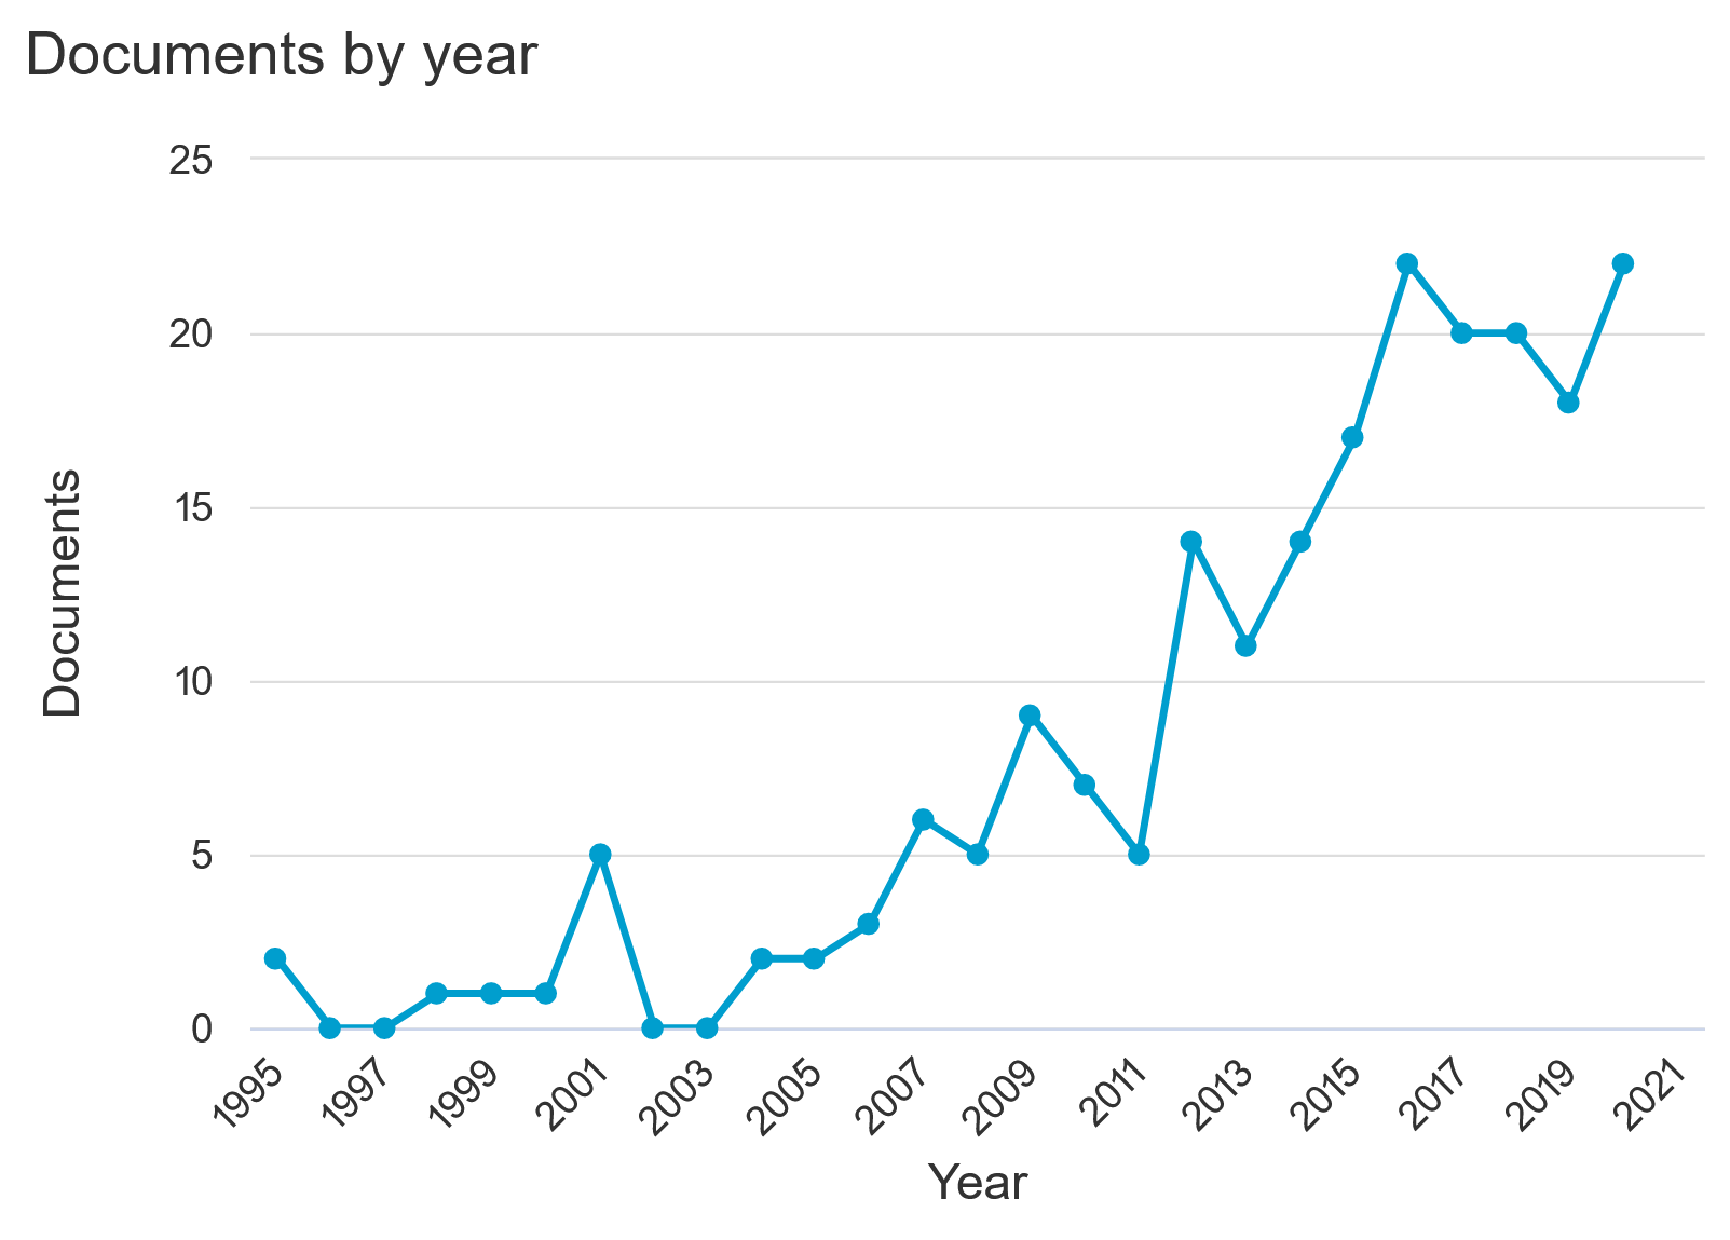
\includegraphics[width=\textwidth]{figures/chap-2/business-needs-hist.pdf}
    \caption{Timeline of the volume of contributions per years for information needs of crisis responders. The year 2021 is excluded because the year is not complete at the time of writing.}
    \label{literature:business-needs-hist}
\end{figure}

The overlay of the keywords generated from the articles retrieved (Figure~\ref{literature:business-needs-overlay}) spans from 2010 to 2018.
It reveals two clusters: one centered on medical issues and another centered on information systems.
The medical cluster focuses on staff well-being and, in particular, on psychological aspects.
The other cluster focuses on emergency services and events management information systems.
This last one is more in connection with the objective of this manuscript; the next analysis will be focused on it.

\begin{landscape}
    \begin{figure}[hp]
        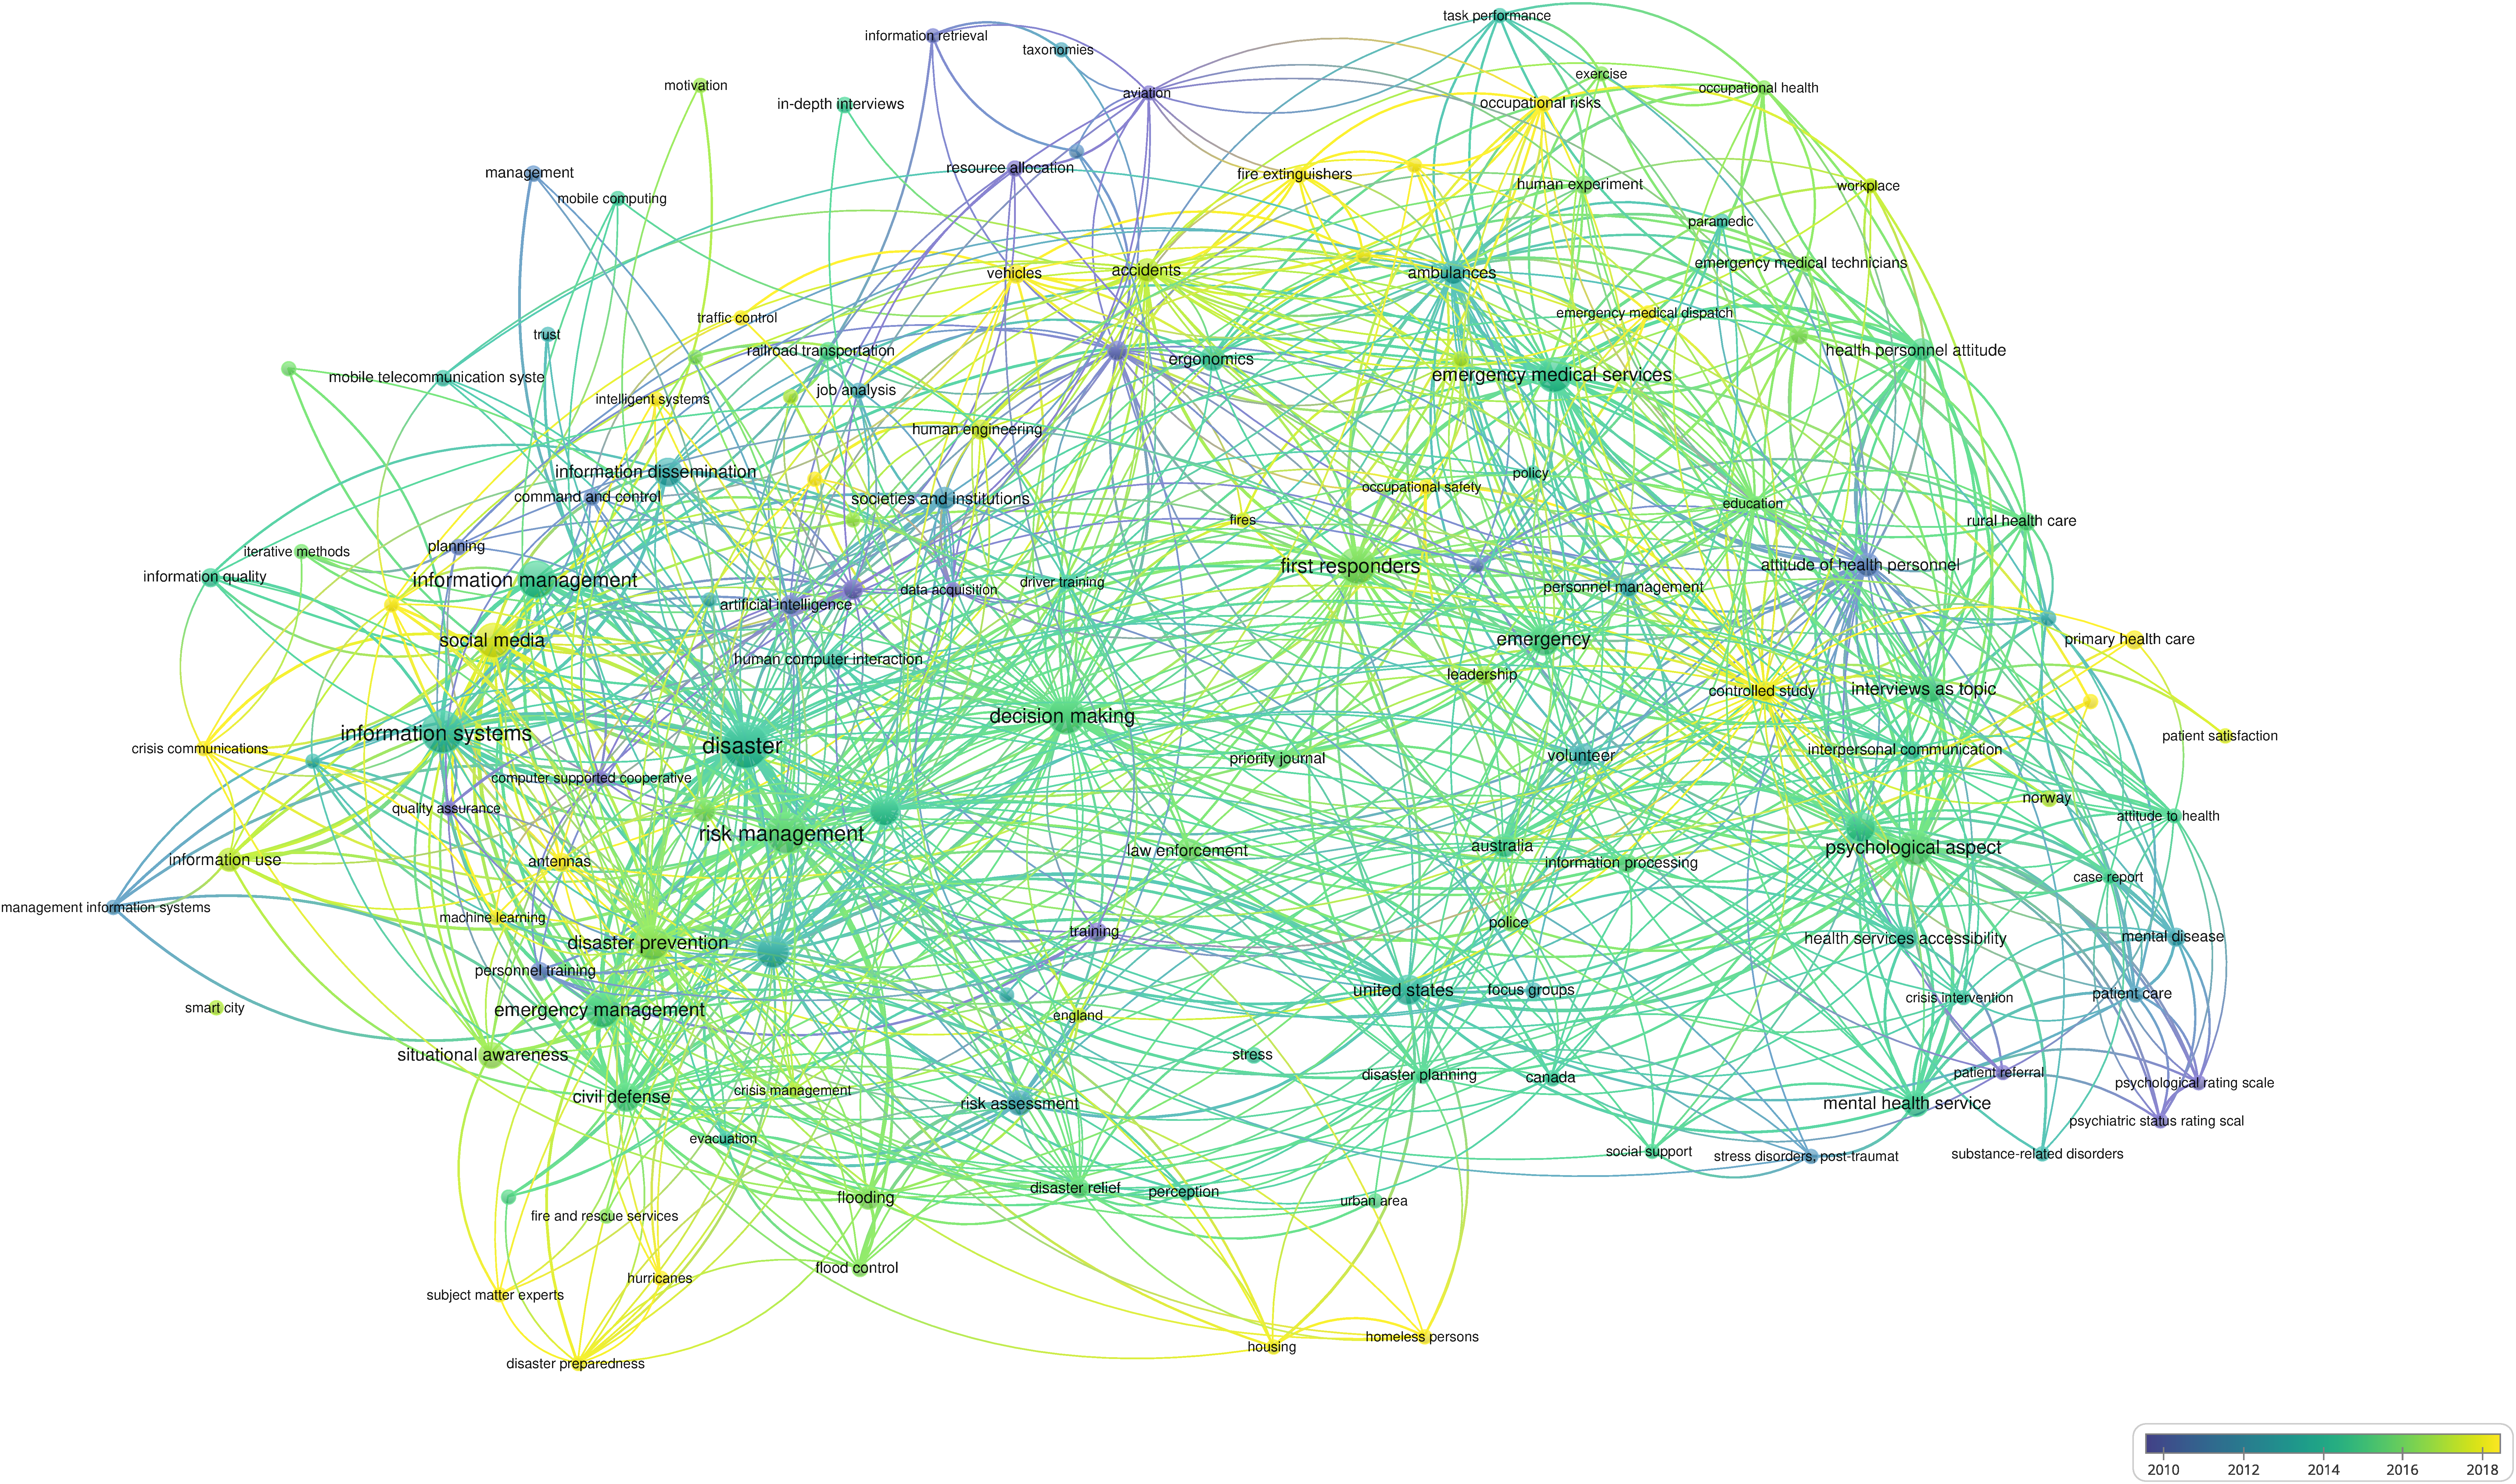
\includegraphics[width=\paperwidth,height=\paperheight,keepaspectratio]{figures/chap-2/business-needs-overlay.pdf}
        \caption{Distribution of keywords with more than 3 occurrences among the articles from the query on information needs of crisis responders.}
        \label{literature:business-needs-overlay}
    \end{figure}
\end{landscape}

The left cluster is composed of the most common keywords used in the fetched articles.
Keywords such as \emph{disaster}, \emph{information systems} and \emph{risk management} (Figure~\ref{literature:business-needs-bar}) are the most prominent ones and seems to be mostly used circa 2014.
Before that period (between 2010 and 2014), the field was primarily focusing on resource or training planning.
But the field took a shift towards data processing to support \emph{decision-making} during emergency events.
The collision with the other domains explored in this chapter seems to happen around 2018, with the use of keywords such as \emph{machine learning}, \emph{social media} or \emph{situational awareness}.

\begin{figure}[thb]
    \centering
    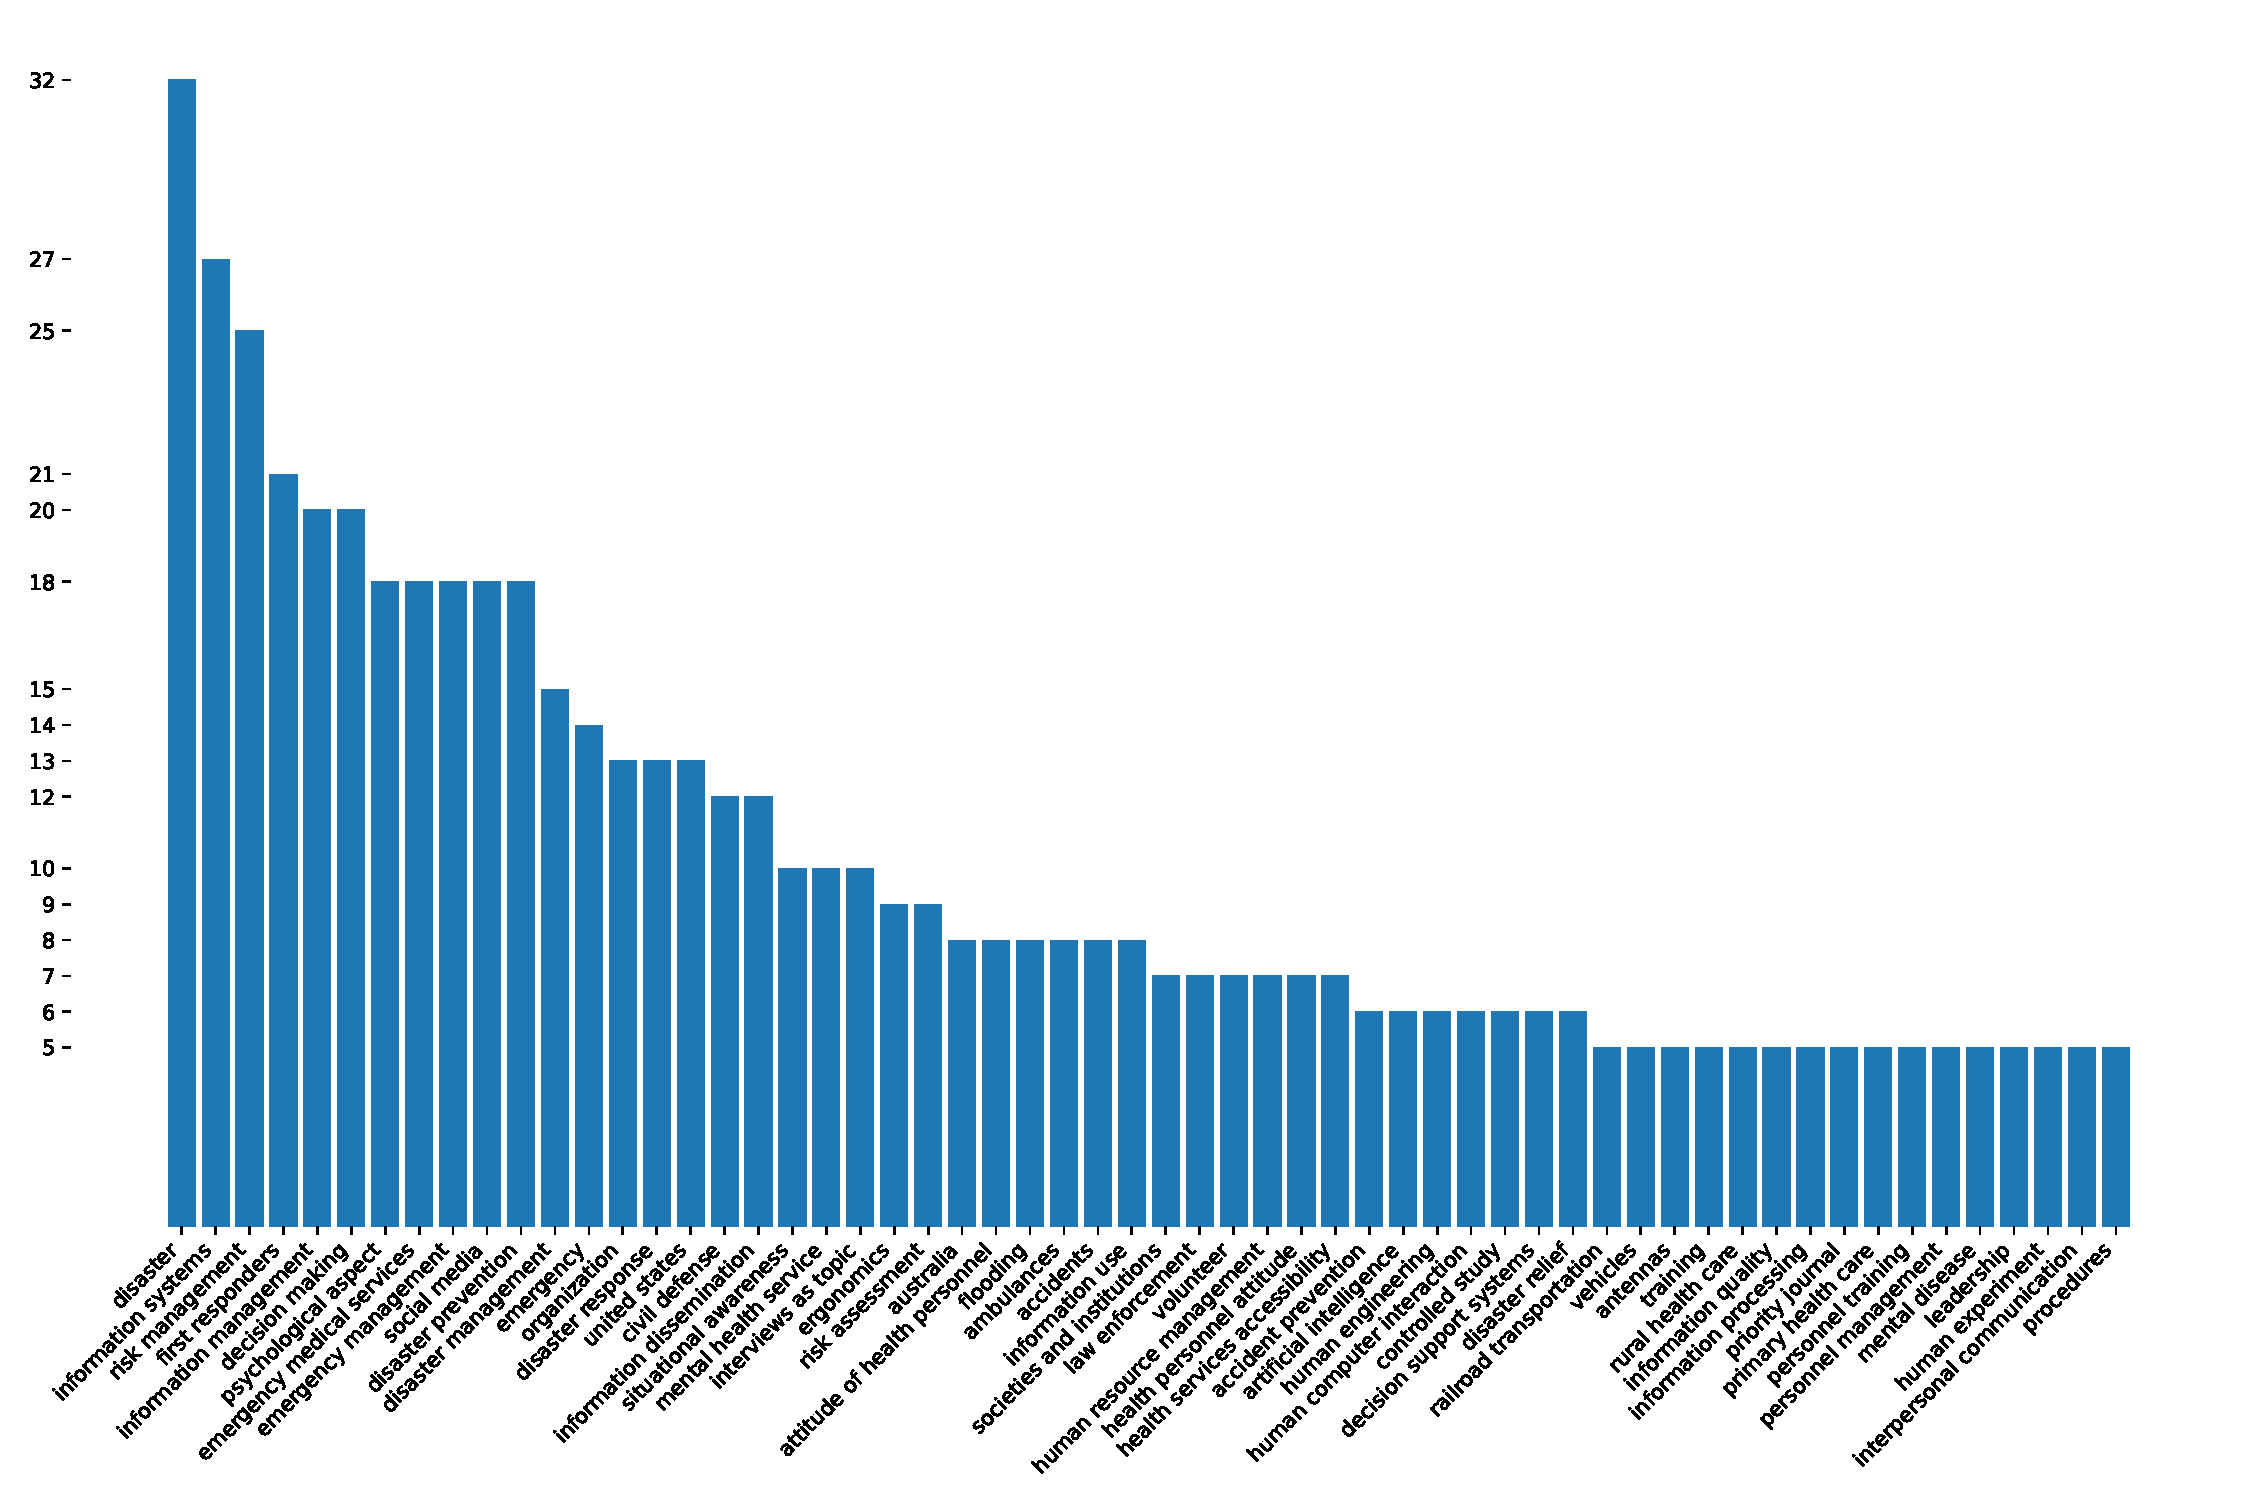
\includegraphics[width=\textwidth]{figures/chap-2/business-needs-bar.pdf}
    \caption{Distribution of keywords with more than 3 occurrences among the articles from the query on information needs of crisis responders.}
    \label{literature:business-needs-bar}
\end{figure}

Table~\ref{table:business-needs-main-articles} provides a summary of the responder's needs identified in the most prominent articles in the field.
Articles were selected if at least 25 citations were published in 2010 or after, are located in the information systems cluster, and are not duplicates.
The articles retrieved provide insights on some of the pain points of emergency organizations.

\begin{table}[bht]
    \centering
    \tabulinesep=1.2mm
    \caption{Articles on informational needs of emergency responders retrieved from the previous request with at least 25 citations.}
    \begin{tabu} to \textwidth {X[1,m]X[3,m]}
        Reference                                                   & Business need identified by the authors.                                                                                                                                                                              \\ [0.5ex]
        \toprule
        \cite{lindellTsunamiPreparednessOregon2010}                 & Tsunami training                                                                                                                                                                                                      \\
        \cite{aloudatRegulationUbiquitousMobile2011}                & Communication to the public                                                                                                                                                                                           \\
        \cite{berlinWhyCollaborationMinimised2011}                  & Collaboration between the different actors                                                                                                                                                                            \\
        \cite{parkerSurfaceWaterFlood2011}                          & Create conversations between unusual actors during the preparation phase                                                                                                                                              \\
        \cite{yangDesignPrinciplesIntegrated2012}                   & Increase situation awareness, Identify key information~\footnote{(hazard environment, information concerning the responder workforce, information on evolving safety issues, and information about safety equipment)} \\
        \cite{tapiaTrustworthyTweetDeeper2013}                      & Accounting for informal sources of data (such as social media)                                                                                                                                                        \\
        \cite{cobbDesigningDelugeUnderstanding2014}                 & Big data processing methods adapted to social media data                                                                                                                                                              \\
        \cite{cabreraaguileraModellingPerformanceVariabilities2016} & Oil spill preparation                                                                                                                                                                                                 \\
        \bottomrule
    \end{tabu}
    \label{table:business-needs-main-articles}
\end{table}

Some studies are event-specific due to a governmental request or a gap in the emergency preparation cover.
\textcite{lindellTsunamiPreparednessOregon2010} is interested in tsunamis management on the US east coast and \textcite{cabreraaguileraModellingPerformanceVariabilities2016} tackle oil spill.
Neither study addresses any particular point in managing this type of event.
Instead, they implement the entire crisis management cycle for these events, which were not considered until their work.
Unfortunately, no specific information needed for decision-makers emerges.

On the other hand, others articles are most focused on the specific needs of emergency organizations.
Collaboration, information sharing and joint preparation exercises are one of the concerns raised \parencite{berlinWhyCollaborationMinimised2011,parkerSurfaceWaterFlood2011}.
The increasing complexity of crisis events asks for a broader range of skills.
As no organization can possess all the required skills simultaneously, other actors must be involved.
Crisis management organizations acknowledge that an unexpected collaboration between actors yields poor outcomes during the response.
Thus, exercises and discussions are critical during the preparation phase, and an adequate means of communication between the actors during the response are needs identified by the studies.

\textcite{yangDesignPrinciplesIntegrated2012} highlight an interesting and well-mentioned need for crisis response: situation awareness.
Situation awareness corresponds to the representation of the state of the environment that surrounds the emergency response organization during an event.
This representation directly guides decision-making.
Consequently, it is critical to build the best and most accurate representation possible at the event's start.
In there are articles, \citeauthor{yangDesignPrinciplesIntegrated2012} emphasize 4 critical pieces of information for situational awareness:

\begin{enumerate}
    \item Environmental conditions such as the building infrastructure, number of occupants, and the exact location of any hazards;
    \item Information on the response participants such as who is involved in the response, what skills they could offer, and what resources they bring to the scene;
    \item The status of any casualties, the accident location, cause, and severity; and
    \item The available resources, including equipment and food.
\end{enumerate}

As per the authors, "timeliness, accuracy, and completeness are the critical dynamic attributes of these four categories of information."
The next chapter (chapter three) will dive deeper into this concept.

The issue with building an accurate situation awareness is the need for information.
With the disruption of regular communication and information channels, decision-makers are shrouded in darkness.
According to \textcite{tapiaTrustworthyTweetDeeper2013,cobbDesigningDelugeUnderstanding2014}, some emergency centers acknowledge the benefit of social media as a potential information source.
However, the issue identified is the lack of tools and methods, similar to those built for calls for social media.

Finally, the last need identified among the extracted items is communication to the public.
\textcite{aloudatRegulationUbiquitousMobile2011} insist on the potential yielded by modern communication means such as cell phones and social media to share information with the public during an event.
People are not always close to a radio or a TV.
Hence, they often miss critical messages during fast-moving events (floods, fires, etc.), resulting in casualties.
On the other hand, (almost literally) most of the population carry a cellphone nowadays, and the critical messages could be distributed faster and with a better viewing rate than traditional methods.
Text messages or notifications from social media could be more effective communication channels that emergency response teams should use.

\subsection{Gathering information on social media?}
The previous two subsections focused on (i) the representations proposed to describe crises and (ii) the challenges organizations face in charge of crisis management.
The overview of these aspects has remained relatively general.
This sub-section, therefore, proposes to refocus the previous analyses on the articles that specifically mention social media.
It also provides insights on the initial research question: What information can be obtained from social media relevant to decision-makers in crisis response?

The keywords "social media" and "Twitter" have been added to the previous queries to refocus on social media.
In the case of the query on crisis models, 18 articles mention social media among 205 initial documents.
The following presents the different information that authors seek from social media.
Thus, ten of the 18 articles do not specify what information they hope to collect but only mention social media as a potential source.
The findings from the remaining articles are summarized in Table~\ref{table:information-model-social-media}.
% \parencite{pobletCrowdsourcingRolesMethods2018,kemavuthanonIntegratedQuestionansweringSystem2020b,khzamDomainspecificSoftwareLanguage2018,mossgraberSensorDecisionChain2018,laudyRumorsDetectionSocial2017,hayesCareEthicsResponsible2020}
he table highlights the main information that the authors wish to use to implement the ontologies they propose.
Information about the event, such as its type and effects, is the most common information required.
Victims' information is also mentioned in several studies.
Interestingly, the studies seem to fall into two groups.
In the first group, ontologies are created before retrieving posted messages.
In this group, the authors thus seek to filter the messages that correspond to the ontologies they use \parencite{gaurEmpathiOntologyEmergency2019,moiDesignOntologyUse2016,narayanasamyCrisisDisasterSituations2019b,montarnalAutomatedEmergenceCrisis2017,cocheActionableCollaborativeCommon2019c}.
The second group follows a similar approach but proceeds to the first phase of message collection, whose content feeds the ontology construction.
The ontologies thus obtained are then "closer" to social media by "moving away" from crisis management \parencite{kemavuthanonClassificationSocialMedia2020b,kawtrakulImprovingDisasterResponsiveness2012,leeConstructionEventOntology2013}.

\begin{table}[bht]
    \centering
    \tabulinesep=1.2mm
    \caption{Articles on informational needs of emergency responders retrieved from the previous request with at least 5 citations.}
    \begin{tabu} to \textwidth {X[1,m]X[3,m]}
        Reference                                            & Information authors are looking for from social media                       \\ [0.5ex]
        \toprule
        \textcite{purohitIdentifyingSeekersSuppliers2014}    & Victims' needs and people offering resources.                               \\
        \textcite{gaurEmpathiOntologyEmergency2019}          & Location, Event type and impact, Victims, Resource, Actors involved, Status \\
        \textcite{ghahremanlouGeotaggingTwitterMessages2014} & Geographic location                                                         \\
        \textcite{bhattAssistingCoordinationCrisis2014}      & Victims' needs                                                              \\
        \textcite{zavarellaOntologybasedApproachSocial2014}  & Event type, Event impact, Location, Weapon inolved, Organizations involved  \\
        \textcite{cocheActionableCollaborativeCommon2019c}   & Location, Event type, Weapon involved, Victims                              \\
        \textcite{montarnalAutomatedEmergenceCrisis2017}     & Crisis related messages, Event type, Time of publication                    \\
        \textcite{leeConstructionEventOntology2013}          & User name, Time of publication, Location, Event type                        \\
        \bottomrule
    \end{tabu}
    \label{table:information-model-social-media}
\end{table}

The same methodology is then applied to the needs of crisis management organizations.
Adding the keywords \emph{social media} and \emph{Twitter} indicates that 21 of the 219 articles previously retrieved are related to these topics.
Unlike the studies retrieved in the previous query, these rarely consider categories of social media information.
Table~\ref{table:business-needs-social-media} summarizes the different approaches considered in the main articles.
Among these articles are common interests that can be grouped into three categories.
First, the involvement and consideration of volunteers in crisis management \parencite{smithSocialMediaCitizenled2018,graceCommunityCoordinationAligning2018,nielsenEmbracingIntegratingSpontaneous2019,cobbDesigningDelugeUnderstanding2014}.
Another group of studies focuses on filtering information from social media to reduce the volume of information reaching decision-makers.
The aim is to avoid an information overload that would be detrimental to the conduct of the response \parencite{onealTrainingEmergencyresponseImage2019,norri-sederholmEnsuringInformationFlow2017,moiStrategyProcessingAnalyzing2016,kaufholdMitigatingInformationOverload2020}
Finally, the last group focuses on the veracity of social media content and the information they expose to response organizations.
As such, two of the four publications highlight the usefulness of this content for the response, while the other two call for more caution \parencite{mehtaTrustVerifySocial2017,tapiaTrustworthyTweetDeeper2013,tapiaGoodEnoughGood2014,vangorpJustKeepTweeting2015}.

\begin{table}[bht]
    \centering
    \tabulinesep=1.2mm
    \caption{Articles on informational needs of emergency responders retrieved from the previous request with at least 5 citations.}
    \begin{tabu} to \textwidth {X[1,m]X[3,m]}
        Reference                                             & Approach to information from social media                         \\ [0.5ex]
        \toprule
        \textcite{cobbDesigningDelugeUnderstanding2014}       & People requiring or providing resources                           \\
        \textcite{graceCommunityCoordinationAligning2018}     & Consideration of citizen reports posted on social media           \\
        \textcite{kaufholdMitigatingInformationOverload2020}  & Reducing information overload through social media filtering      \\
        \textcite{mehtaTrustVerifySocial2017}                 & Evaluation of uncertainty of information coming from social media \\
        \textcite{moiStrategyProcessingAnalyzing2016}         & Reducing information overload through social media filtering      \\
        \textcite{nielsenEmbracingIntegratingSpontaneous2019} & Considering volunteers in crisis management                       \\
        \textcite{norri-sederholmEnsuringInformationFlow2017} & Importance of information flow to reduce information overload     \\
        \textcite{onealTrainingEmergencyresponseImage2019}    & Image classification to detect rescuers and rescuees              \\
        \textcite{smithSocialMediaCitizenled2018}             & Social media use of volunteers during disaster                    \\
        \textcite{tapiaGoodEnoughGood2014}                    & Evaluation of uncertainty of information coming from social media \\
        \textcite{tapiaTrustworthyTweetDeeper2013}            & Evaluation of the usefulness of social media content              \\
        \textcite{vangorpJustKeepTweeting2015}                & Evaluation of the usefulness of social media content              \\
        \bottomrule
    \end{tabu}
    \label{table:business-needs-social-media}
\end{table}

This section has gone through different aspects of the research question: \emph{What can decision-relevant information from social media be processed automatically?}
The first two sections have explored information processing in crisis management globally along two axes.
The first axis is the crisis models designed and proposed by computer sciences.
We have seen that a great diversity of models have been proposed.
This diversity mainly results from the granularity or scale adopted by the authors or the type of disaster studied.
The second axis has adopted the point of view of the social sciences on these issues.
The latter has allowed us to understand the numerous issues of emergency organizations in managing their information.
The final part of this section focused on the studies from both approaches that considered social media as a source of information.
In this context, most of the research from the computer science community focused on implementing different ontologies proposed.
The teams that presented the information that was attempting to retrieve mostly focused on the following information:

\begin{itemize}
    \item Event type
    \item Event consequences
    \item Victims status
    \item Victims needs
    \item Location
\end{itemize}

On the other hand, social studies are less interested in what information is processed but rather in how it is processed.
Three main topics appear from the set of studies highlighted in this part.
First, consider physical and digital volunteers in crisis response and include them in the official process.
Secondly, managing the flow of information to avoid information overload.
This research group is directly aligned with the views of the computer science domain.
The final research group focuses on assessing the value of social media information for crisis management.
Interestingly, each axis has a different approach to managing social media information during crisis response.
The first axis took a top-down approach by thinking about representations that are then confronted with reality.
The second axis took the other direction, with a bottom-up approach, where authors interview practitioners to identify points of interest.
This section highlighted the need and previous attempts to automate the collection and management involved in crisis management.
Also, it showed that social media are a source of valuable information that requires appropriate means of processing.
Thus, the following section discusses existing means of identifying and mining information from social media.

\section{NLP methods for information extraction from social media data}
The first chapter presented the Natural Language Processing (NLP) domain.
Through the development of this domain, many tools, algorithms, and methods have been developed to process textual data.
With the emergence of social media, a new source of textual data appeared, and with it, its own challenges.
This chapter explores the following research question: \emph{How can this information be obtained in the context of crisis informatics?}
Social media data are used as a data source in various use cases.
This section is broken down into two parts, and it aims to explore two directions.
First, for which applications is NLP used on social media data?
Secondly, what are the methods used to extract information from social media?
Each question is treated in a sub-section.
To explored these two direction the following request is run:

\begin{table}[bht]
    \centering
    \tabulinesep=1.2mm
    \caption{Overview of the bibliographic request related to challenges in crisis management.}
    \begin{tabu} to \textwidth {X[0.5,r]X[1,m]X[1,m]}
        Type of request & Keywords                                                            & Explaination                                                                      \\ [0.5ex]
        \toprule
        SUBJAREA        & \textit{comp}                                                       & Articles in either Computer Science, Social Sciences of Decision Sciences domains \\
        TITLE-ABS-KEY   & \textit{natural language processing} OR \textit{information mining} & Articles focus on natural language processing or information mining               \\
        TITLE-ABS-KEY   & \textit{social media} OR \textit{Twitter}                           & To process social media data                                                      \\
        TITLE-ABS-KEY   & \textit{survey}                                                     & Only surveys are considered in this section                                       \\
        EXCLUDE-DOCTYPE & \textit{re} OR \textit{cr}                                          & Reviews and conference tracks introductions are excluded                          \\
        \bottomrule
    \end{tabu}
    \label{table:nlp-challenges}
\end{table}

This section will only consider surveys published in the domain.
This choice is made to filter the numerous publications in this area.
Without this constraint, the request returns 4231 documents.
This large volume of publications, which reflects the popularity of the field, makes it challenging to analyze the field's evolution.
However, restricting the results in this way should not prevent reporting on trends in the field.
The request presented in Table~\ref{table:nlp-challenges} returns 217 surveys, published between 2011 and 2021 (Figure~\ref{literature:nlp-hist}).
While being a relatively recent research venue, the interest in NLP uses on social media data has increased over the years.

\begin{figure}[thb]
    \centering
    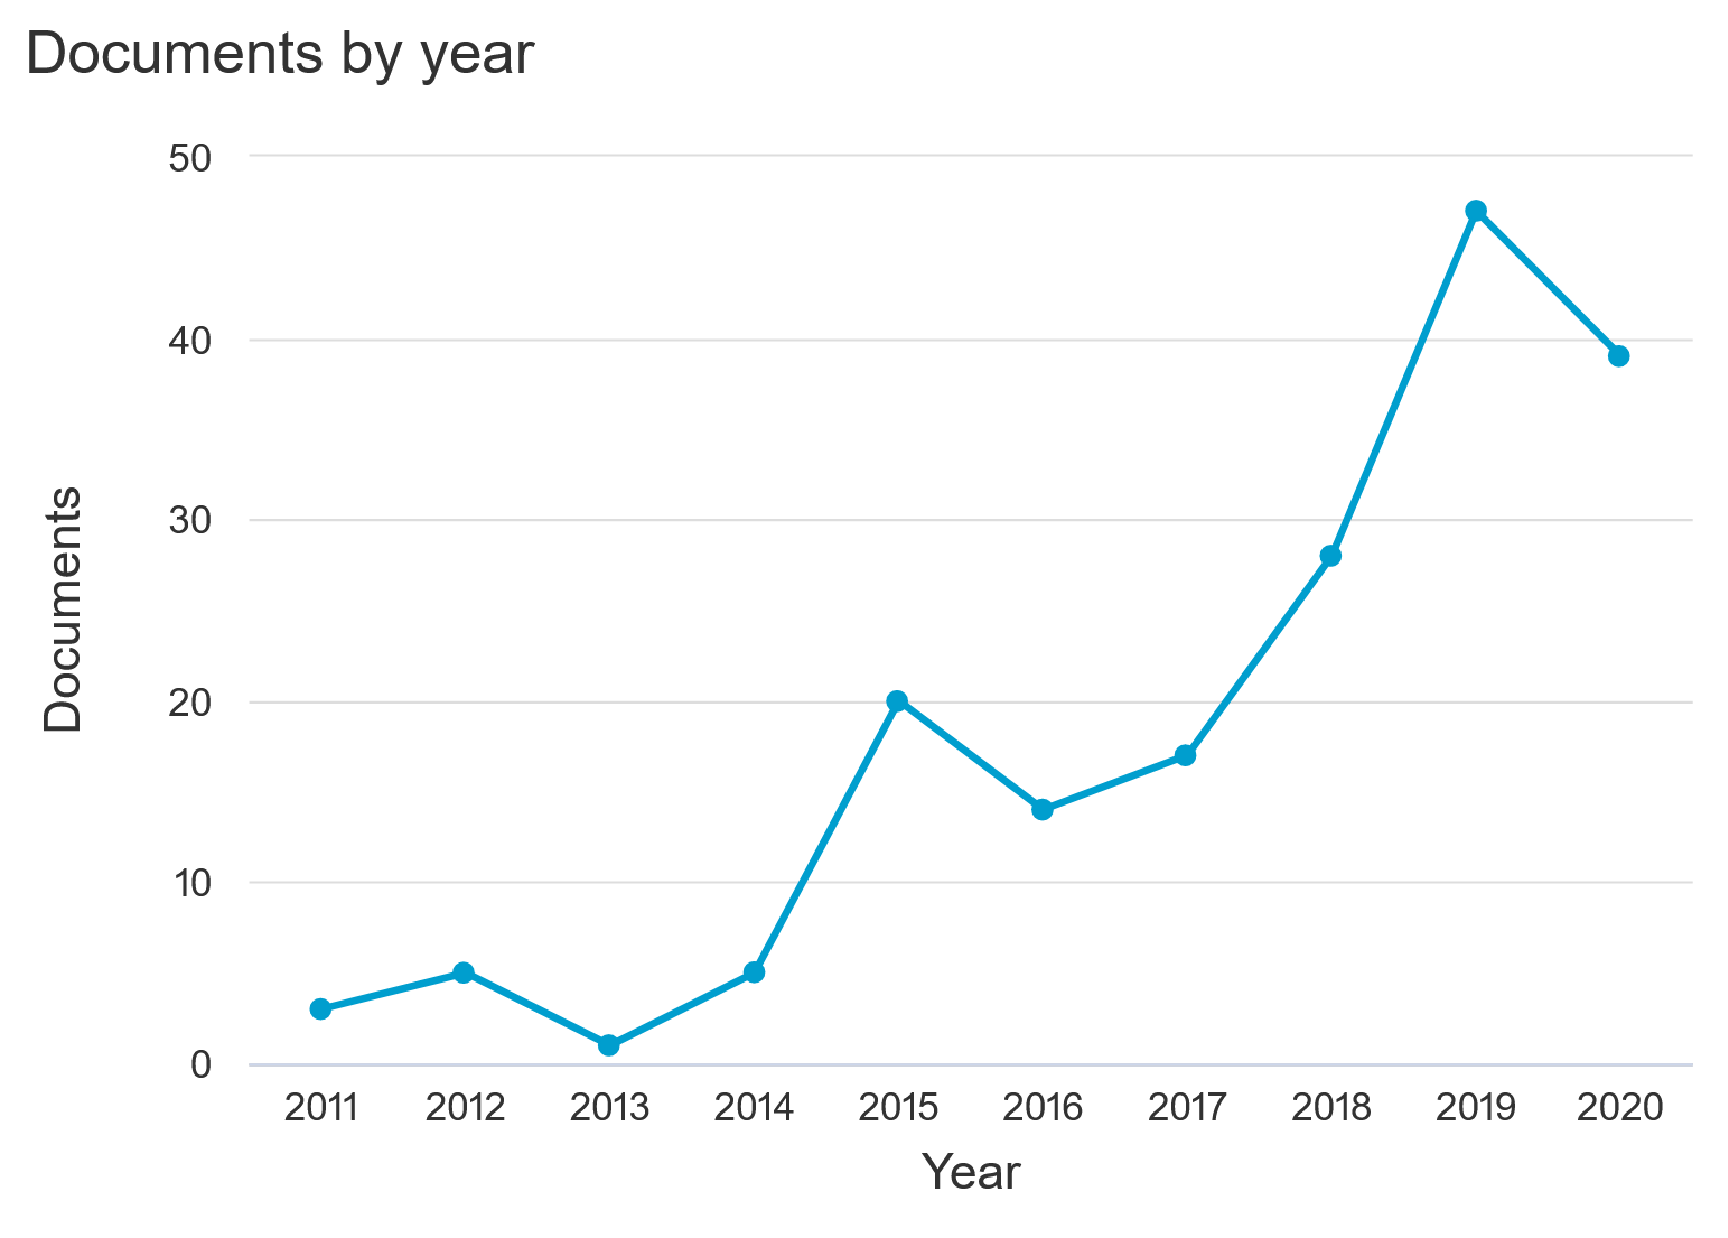
\includegraphics[width=\textwidth]{figures/chap-2/nlp-hist.pdf}
    \caption{Timeline of the volume of contributions per years for the application of NLP methods to social media data. The year 2021 is excluded because the year is not complete at the time of writing.}
    \label{literature:nlp-hist}
\end{figure}

The surveys retrieved appear as a single cluster (Figure~\ref{literature:nlp-overlay}).
This overlay was created by aggregating synonyms, removing the keywords from the query, and some keywords with a low value for our study ("state of the art, large amounts, codes (symbols), research questions, text").
Despite the field's youth, its evolution is swift, both in applications and methods used.
Circa 2011, the field was centered around epidemiological applications and statistical analyses.
From this point on, a kaleidoscope of applications and methods was used.
They are detailed in the following two subsections.

\begin{landscape}
    \begin{figure}[hp]
        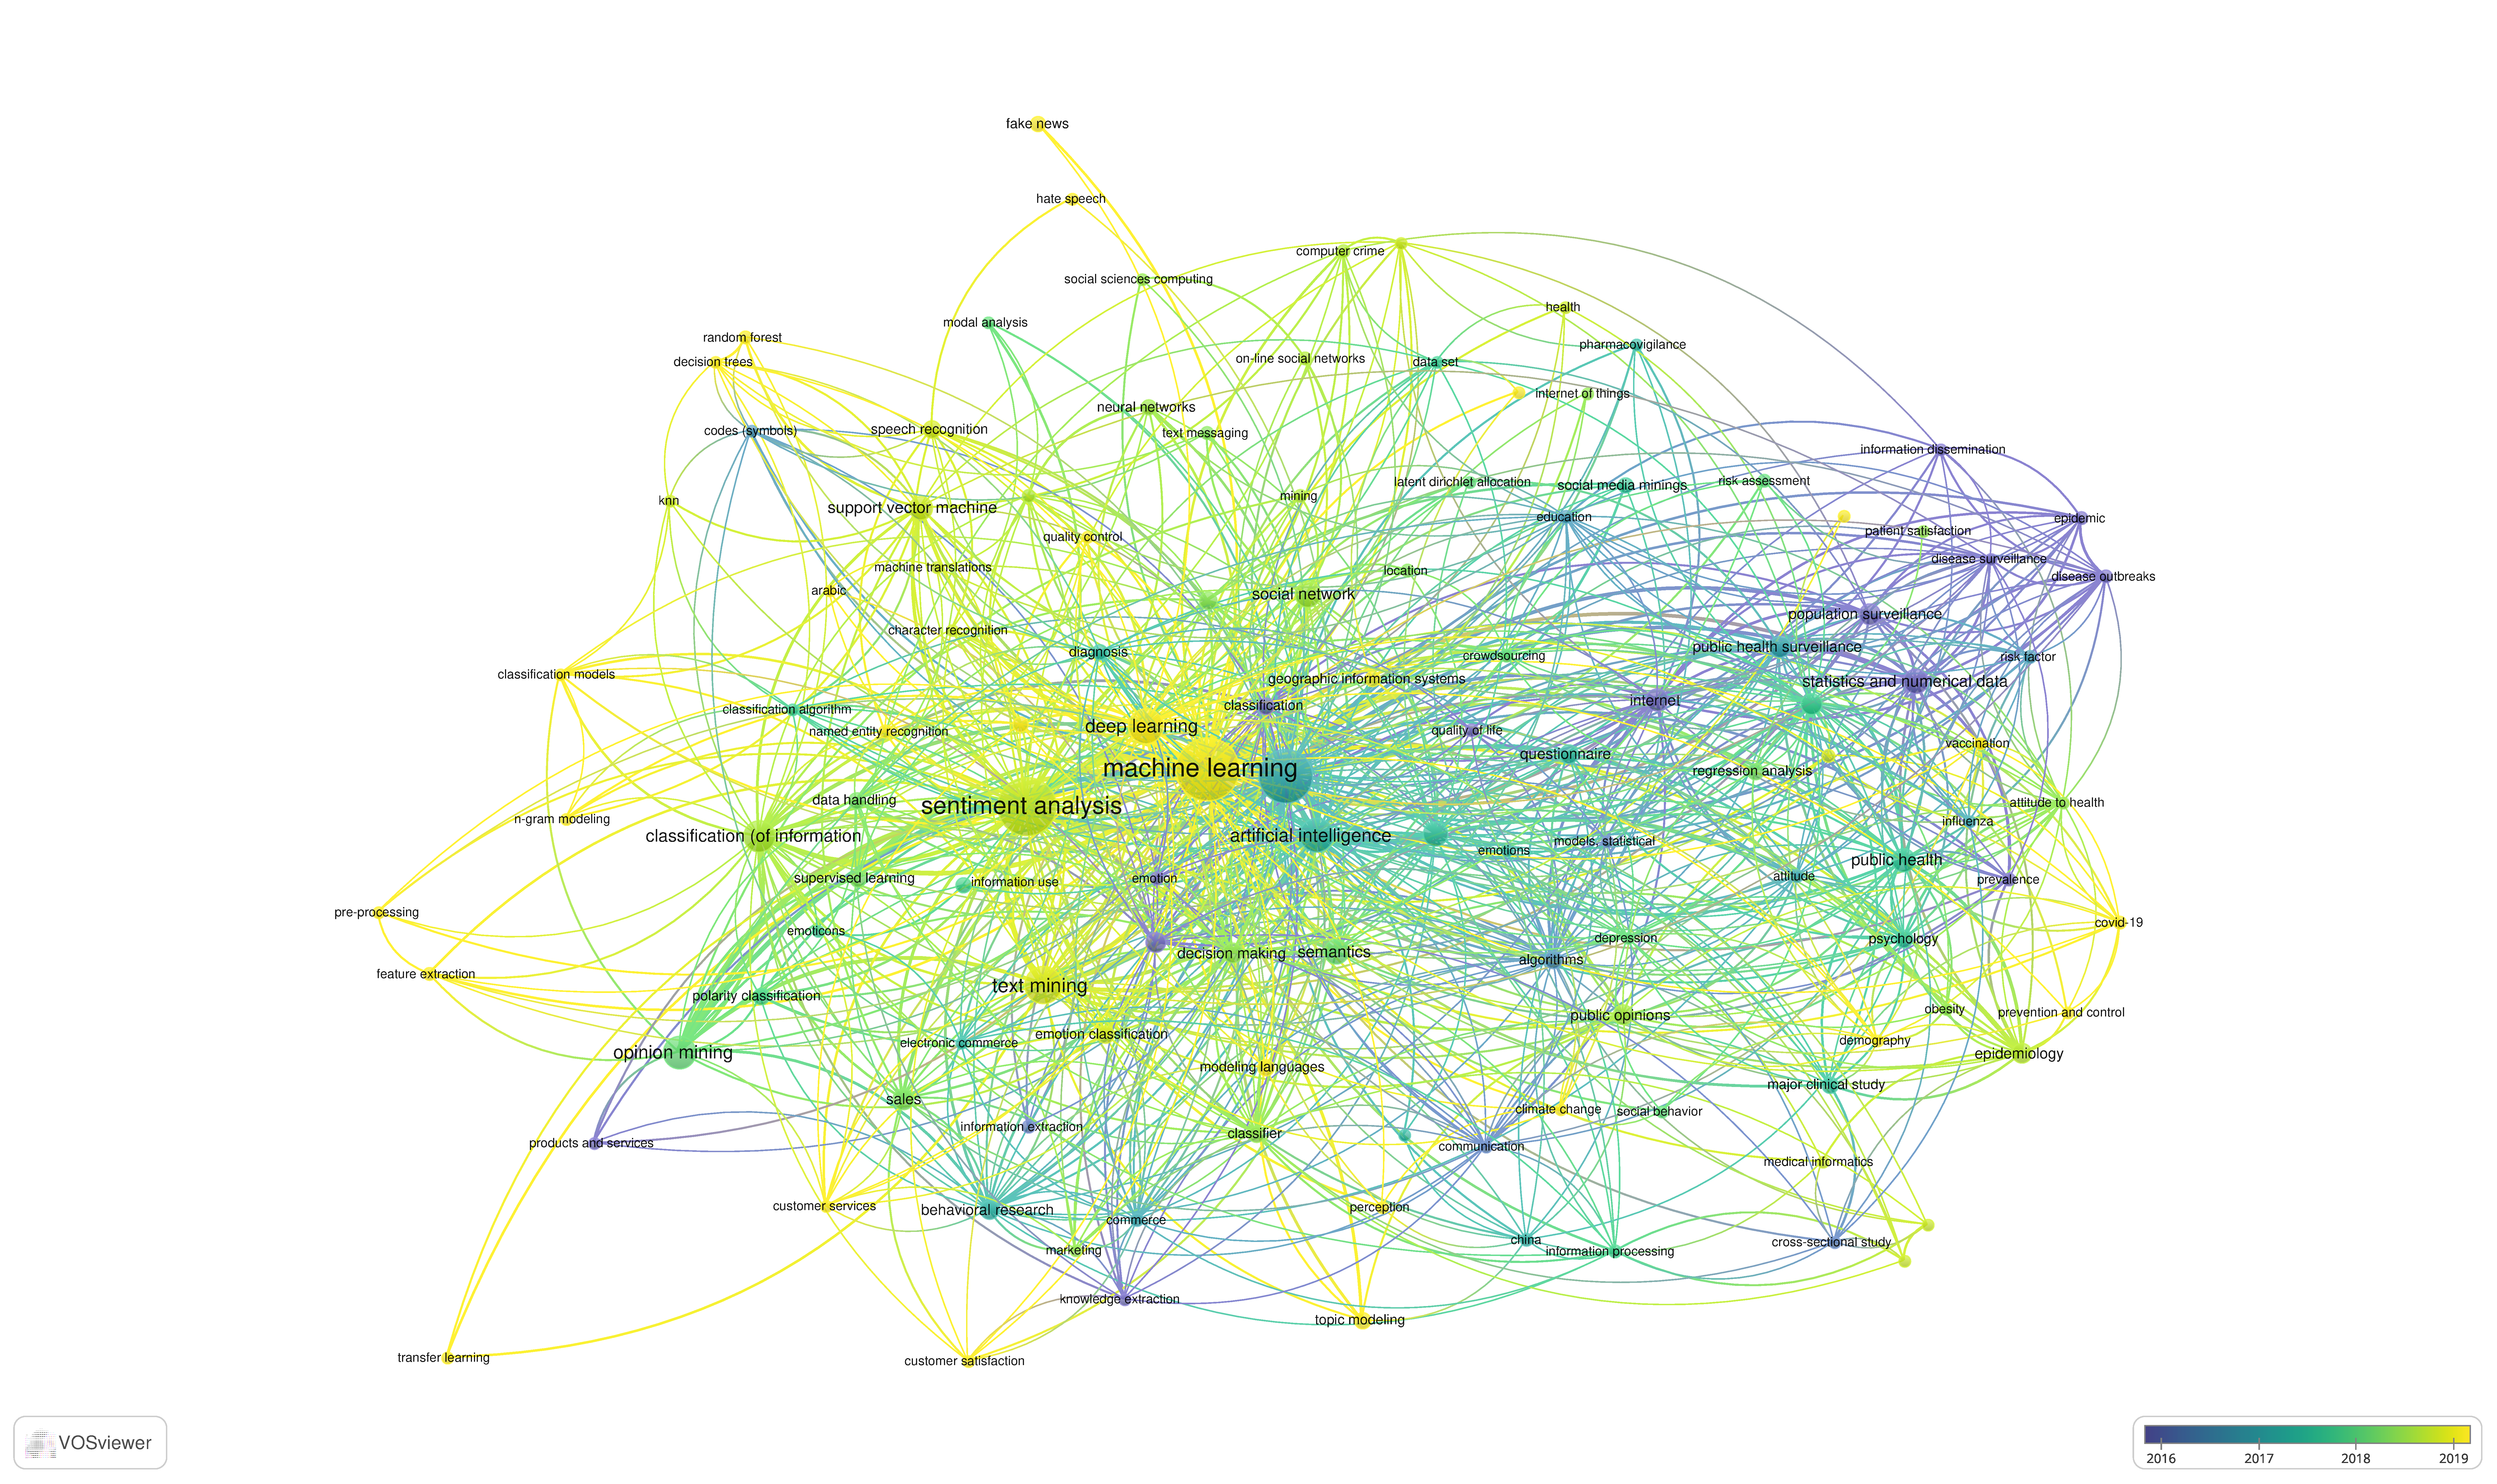
\includegraphics[width=\paperwidth,height=\paperheight,keepaspectratio]{figures/chap-2/nlp-overlay.pdf}
        \caption{Distribution of keywords with more than 3 occurrences among the articles from the query on NLP applied on social media data.}
        \label{literature:nlp-overlay}
    \end{figure}
\end{landscape}

However, some keywords trends have been more prominent during these years than others.
On the application side, \emph{sentiment analyses} is by far the most studied application (73 mentions of this keyword) (Figure~\ref{literature:nlp-bar}).
Mining applications are second with \emph{data mining} (mentioned 61 times), \emph{text mining} (30 times) and \emph{opinion mining} (mentioned 21 times).
On the method side, \emph{artificial intelligence} (mentioned 25 times), and especially \emph{machine learning} (85 times, almost half surveys) methods (such as shown with the appearance of \emph{deep learning}) are heavily mentioned as well in the surveys.
These methods illustrate the importance of the applications of machine learning methods in natural language processing.

\begin{figure}[thb]
    \centering
    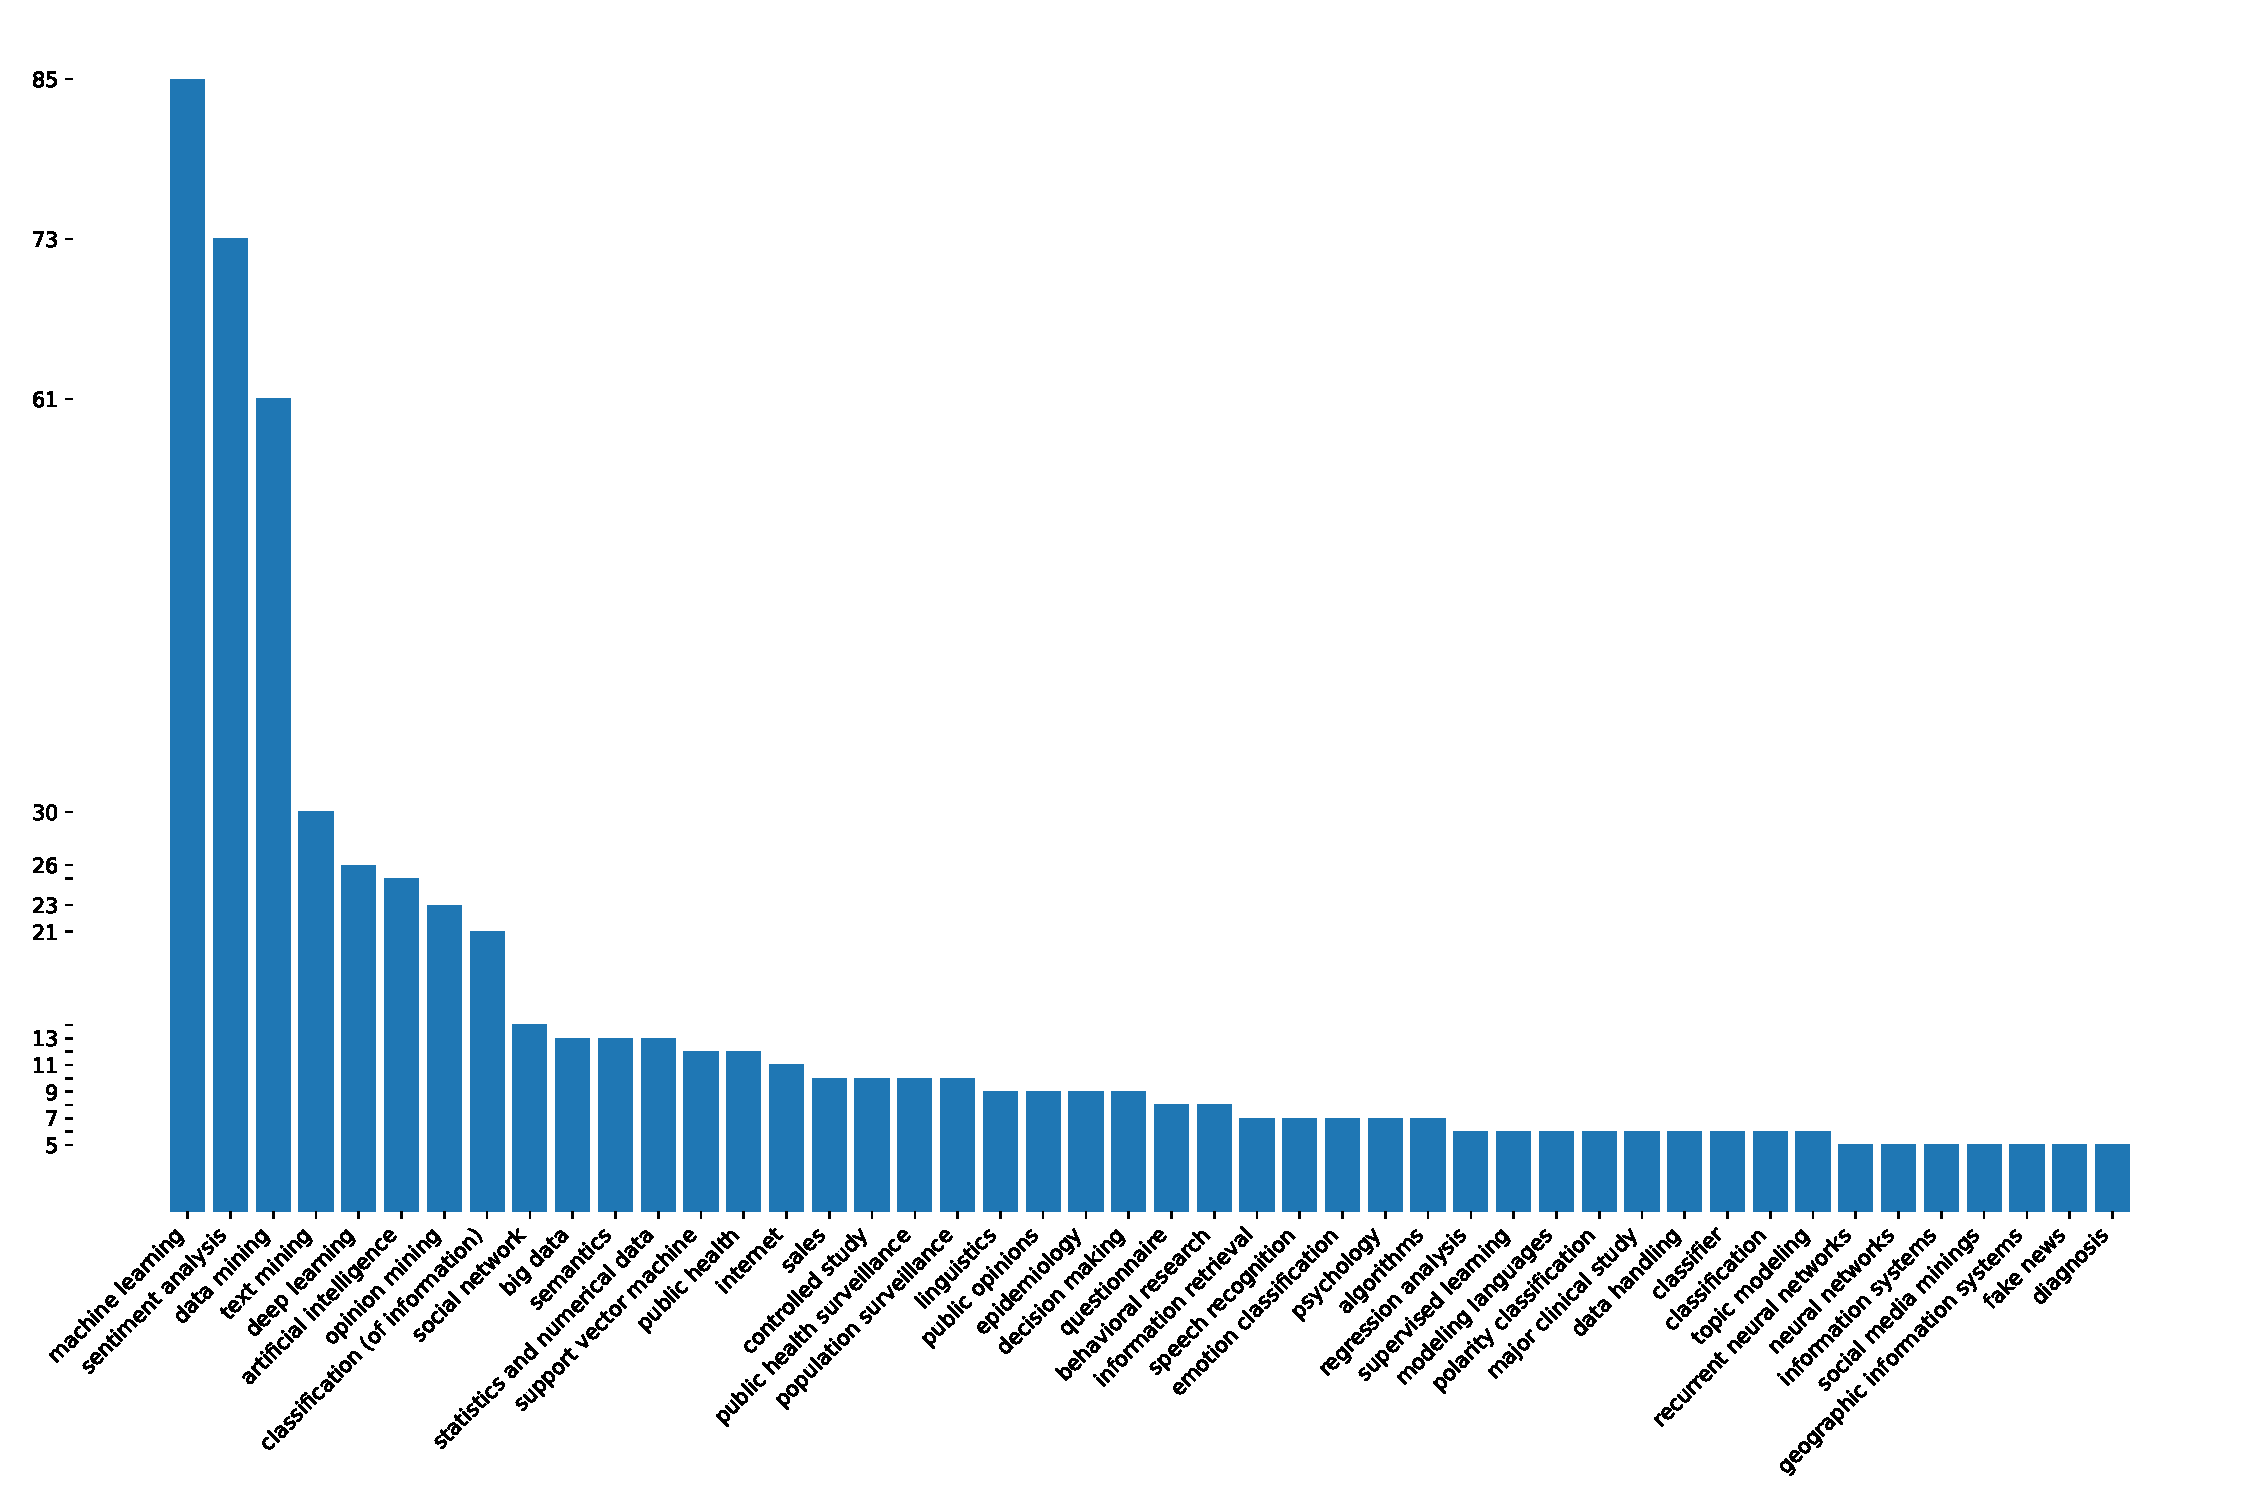
\includegraphics[width=\textwidth]{figures/chap-2/nlp-bar.pdf}
    \caption{Distribution of keywords with more than 4 occurrences among the articles from the query on NLP applied on social media data.}
    \label{literature:nlp-bar}
\end{figure}

Table~\ref{table:nlp-main-articles} presents the main surveys, their focus, and the associated field of application.
Specifically, 27 surveys cited more than 25 times appear.
These 27 documents are divided into seven topics:

\begin{itemize}
    \item Sentiment analysis
    \item Epidemiology
    \item Health
    \item Text mining
    \item Social Network
    \item Uncertainty
\end{itemize}

Nine surveys compose the sentiment analysis topic \parencite{yadavSentimentAnalysisUsing2020,hemmatianSurveyClassificationTechniques2019,chaturvediDistinguishingFactsOpinions2018,raviSurveyOpinionMining2015,chamlertwatDiscoveringConsumerInsight2012,liuSurveyOpinionMining2012,jiangAssessmentOnlinePublic2016,hawkinsMeasuringPatientperceivedQuality2016}.
It is a well-discussed topic as surveys span from 2012 to 2020.
The main objective of sentiment analysis is usually to detect if a message is positive or negative about the topic of the message.
Emotion detection is the next step after sentiment analysis.
It can be more challenging, as it is required to classify text messages to a large variety of emotions that are notably hard to capture \parencite{sailunazEmotionDetectionText2018,poriaReviewAffectiveComputing2017}.
These two subjects make up almost half of the volume of publications highlighted.
Eight articles are related to medical topics.
Four are using social media to study the spread of diseases among the population such as influenza \parencite{kagasheEnhancingSeasonalInfluenza2017,santillanaCombiningSearchSocial2015}, Ebola \parencite{odlumWhatCanWe2015}, and opioids \parencite{charyEpidemiologyTweetsEstimating2017}.
Three others survey the public behavior related to depression \parencite{yazdavarSemiSupervisedApproachMonitoring2017,khzamDomainspecificSoftwareLanguage2018} and to inflammatory disease \parencite{martinezPatientUnderstandingRisks2017}.
Four surveys identify the various approaches available and used in different contexts.
\textcite{salloumSurveyTextMining2017} review different existing methods, while \textcite{paulSocialMediaMining2016} focuses on applications to public health, \textcite{wangSocialMediaSensor2015} on air quality and \textcite{collierUncoveringTextMining2012} epidemiology.
NLP applied to social media also provides valuable insights on social media themselves or the social network of its users.
Three surveys are focusing on these aspects, with \textcite{bailCombiningNaturalLanguage2016} studying advocacy groups and \textcite{vazquezClassificationUsergeneratedContent2014} consumer behavior while \textcite{bontchevaMakingSenseSocial2014} identify semantic relationships between the users.
Finally, the last two surveys remaining study the uncertainty and ambiguity of information posted on social media, with \textcite{haririUncertaintyBigData2019} discussing uncertainty at large in big data and \textcite{linUncertaintyAnalysisCrowdsourced2015} emphasizing on uncertainty on growdsourced reports.

\begin{table}[bht]
    \centering
    \tabulinesep=1.2mm
    \caption{Articles on applications of NLP on social media data retrieved from the previous request with at least 25 citations.}
    \begin{tabu} to \textwidth {X[1,m]X[3,m]}
        Reference                                                & Topic of the survey  (application domain)   \\ [0.5ex]
        \toprule
        \textcite{yadavSentimentAnalysisUsing2020}               & Sentiment analysis (methods)                \\
        \textcite{hemmatianSurveyClassificationTechniques2019}   & Sentiment analysis (methods)                \\
        \textcite{haririUncertaintyBigData2019}                  & Uncertainty (big data analytic)             \\
        \textcite{sailunazEmotionDetectionText2018}              & Emotion detection (methods)                 \\
        \textcite{chaturvediDistinguishingFactsOpinions2018}     & Sentiment analysis (methods)                \\
        \textcite{yazdavarSemiSupervisedApproachMonitoring2017}  & Public health (depression)                  \\
        \textcite{salloumSurveyTextMining2017}                   & Text mining (methods)                       \\
        \textcite{poriaReviewAffectiveComputing2017}             & Emotion detection (methods)                 \\
        \textcite{martinezPatientUnderstandingRisks2017}         & Public health (inflammatory bowel disease)  \\
        \textcite{kagasheEnhancingSeasonalInfluenza2017}         & Epidemiology (influenza)                    \\
        \textcite{charyEpidemiologyTweetsEstimating2017}         & Epidemiology (opioid)                       \\
        \textcite{paulSocialMediaMining2016}                     & Text mining (public health)                 \\
        \textcite{jiangAssessmentOnlinePublic2016}               & Sentiment analysis (infrastructure projets) \\
        \textcite{hawkinsMeasuringPatientperceivedQuality2016}   & Sentiment analysis (quality of care)        \\
        \textcite{bailCombiningNaturalLanguage2016}              & Social network dynamic (advocacy groups)    \\
        \textcite{bahkPubliclyAvailableOnline2016}               & Sentiment analysis (vaccines)               \\
        \textcite{wangSocialMediaSensor2015}                     & Text mining (air quality)                   \\
        \textcite{santillanaCombiningSearchSocial2015}           & Epidemiology (influenza)                    \\
        \textcite{raviSurveyOpinionMining2015}                   & Sentiment analysis (methods)                \\
        \textcite{odlumWhatCanWe2015}                            & Epidemiology (ebola)                        \\
        \textcite{linUncertaintyAnalysisCrowdsourced2015}        & Uncertainty (growdsourcing)                 \\
        \textcite{karmenScreeningInternetForum2015}              & Public health (depression)                  \\
        \textcite{vazquezClassificationUsergeneratedContent2014} & Social network dynamic (consumer behavior)  \\
        \textcite{bontchevaMakingSenseSocial2014}                & Social network dynamic (semantics)          \\
        \textcite{liuSurveyOpinionMining2012}                    & Sentiment analysis (methods)                \\
        \textcite{collierUncoveringTextMining2012}               & Text mining (epidemiology)                  \\
        \textcite{chamlertwatDiscoveringConsumerInsight2012}     & Sentiment analysis (consumer behavior)      \\
        \bottomrule
    \end{tabu}
    \label{table:nlp-main-articles}
\end{table}

The following sub-section explores the applications mentioned by the surveys obtained from the request.

\subsection{Social media information extracted using NLP}
Social media data contain valuable information for a wide range of applications.
The recovered surveys reflect the diversity of application areas.
Table~\ref{table:application-domains} presents the keywords used to build the overlay in Figure~\ref{literature:nlp-overlay}.
These keywords are then associated with domains similar to the previous table.
Here, broader categories are used to account for the more extensive diversity.
For instance, as \emph{sentiment analysis} is used as a keyword, it can hardly be used as a category itself.
Also, some keywords are generic, hence common to multiple domains.
For instance, \emph{attitude} is used both in health and business-related surveys.
\emph{quality of life} is used in urban issues, breast cancers, depression detection, and opioid side effects.
Other keywords that did not belong to any significant category have been grouped separately.
These applications are then grouped into major domains of applications.
This results in seven major application domains identified:

\begin{itemize}
    \item Epidemiology: efforts to track and document an outbreak through social media
    \item Health: tracking of symptoms, psychological distress or drugs mentions
    \item General Public: uses of social media as part of the smart city to prevent crime or collect the public's opinions
    \item Social Media/Social Network: social studies on social media platforms themselves or social interactions through social media
    \item Business: uses of social media for product marketing or maintaining a relationship with consumers.
    \item Information Science: general topic related to extraction and management of information from social media in general
    \item NLP Tasks: a set of tasks related to natural language processing such as translation, speech recognition, etc.
\end{itemize}

The following details some of the most prominent keywords retrieved.
NLP applied to social media is used for a variety of medical applications.
Epidemiology, which studies the distribution and frequency of diseases, uses social media to monitor symptoms related to an epidemic to infer future propagation.
This includes, of course, the COVID-19 outbreak or the 2009-2010 influenza outbreak.
Broader medical applications are labeled under "Medical Informatics."
It contains applications using the same methodology but applied to other diseases or conditions, such as \emph{depression}, \emph{obesity} or \emph{pregnancy}.
Social media are also considered for \emph{pharmacovigilance} to monitor secondary effects (\emph{patient satisfaction}, \emph{opiate addiction}).
The behavior of the urban population (\emph{smartcity}, \emph{computer crime}) or society in general (\emph{demography}, \emph{population surveillance}) can also be observed through social media.
Their feelings about events or political decisions can then be quantified and analyzed.
As digital twins of society, social media are also environments that bring some reflections of their own.
The phenomenon of \emph{fake news} in particular has taken many actors in society by surprise and is an issue that attracts a lot of attention.
How information spreads within the \emph{social network} of users or its very structure are also topics of research.
Marketing departments and Public Relations firms are also naturally very interested in the insights available on social media.
The management of the content of social media and especially the \emph{information extraction} and \emph{knowledge extraction} part
are challenges for the information science domain.
Social media data also come with specific challenges for the NLP domain.
Social media content is noisy, informal, and often comes with its own use of grammar.
Consequently, most of the methods applied to other texts are disrupted with social media data.
\emph{machine translation}, \emph{named entity recognition} and other tasks are then explored and improved in this context.
Alongside improvements on several tasks, social media are also widely used to \emph{sentiment analysis}, \emph{topic modeling} or \emph{polarity classification}.
In the final category, interesting topics appear, such as \emph{crowdsourcing}.
Indeed, instead of exploiting social media, some social scientists leverage their power to achieve goals and then study mechanisms that can encourage positive actions.
Of course, \emph{climate change} is also an application mentioned, considering the importance of this topic.

\begin{center}
    \begin{longtable}{rl}
        \caption{Grouping of the main keywords returned into domains.} \\
        Keyword                         & Domain                       \\
        \bottomrule
        COVID-19                        & Epidemiology                 \\
        disease outbreaks               &                              \\
        disease surveillance            &                              \\
        vaccination                     &                              \\
        epidemic                        &                              \\
        epidemiology                    &                              \\
        influenza                       &                              \\
        opiate addiction                &                              \\
        opioid-related disorders        &                              \\
        depression                      & Health                       \\
        diagnosis                       &                              \\
        psychology                      &                              \\
        public health surveillances     &                              \\
        health survey                   &                              \\
        risk factor                     &                              \\
        major clinical study            &                              \\
        medical informatics             &                              \\
        obesity                         &                              \\
        pregnancy                       &                              \\
        patient satisfaction            &                              \\
        pharmacovigilance               &                              \\
        prevention and control          &                              \\
        quality control                 &                              \\
        risk assessment                 &                              \\
        controlled study                &                              \\
        prevalence                      &                              \\
        social behavior                 & General Public               \\
        models, statistical             &                              \\
        computer crime                  &                              \\
        public opinion                  &                              \\
        population surveillance         &                              \\
        demography                      &                              \\
        smart city                      &                              \\
        risk assessment                 &                              \\
        internet of things              &                              \\
        facebook                        & Social Media/Social Netword  \\
        social media mining             &                              \\
        social network                  &                              \\
        fake news                       &                              \\
        modal analysis                  &                              \\
        data mining                     &                              \\
        information dissemination       &                              \\
        opinion mining                  &                              \\
        perception                      &                              \\
        crowdsourcing                   &                              \\
        surveys and questionnaires      &                              \\
        commerce                        & Business                     \\
        customer services               &                              \\
        sales                           &                              \\
        communication                   &                              \\
        electronic commerce             &                              \\
        marketing                       &                              \\
        products and services           &                              \\
        knowledge extraction            & Information Science          \\
        information systems             &                              \\
        classification (of information) &                              \\
        gis                             &                              \\
        decision-making                 &                              \\
        information extraction          &                              \\
        information processing          &                              \\
        spatiotemporal analysis         &                              \\
        machine translations            & NLP Tasks                    \\
        speech recognition              &                              \\
        polarity classification         &                              \\
        location inference              &                              \\
        text mining                     &                              \\
        automated detection             &                              \\
        named entity recognition        &                              \\
        arabic languages                &                              \\
        linguistics                     &                              \\
        topic modeling                  &                              \\
        emotion analysis                &                              \\
        sentiment analysis              &                              \\
        emoticons                       &                              \\
        modeling languages              &                              \\
        quality of life                 & No specific domain           \\
        china                           &                              \\
        education                       &                              \\
        climate change                  &                              \\
        attitude                        &                              \\
        \bottomrule
        \label{table:application-domains}
    \end{longtable}
\end{center}

\subsection{Overview of NLP's methods}
The previous sub-section presented the different applications of NLP on social media data.
The surveys retrieved also mentioned algorithms, methods, or models related to NLP.
This sub-section aims to present the different methods mentioned briefly.
Table~\ref{table:nlp-tools} shows the keywords used in the surveys and groups them according to the different fields of artificial intelligence to which they belong.

\begin{table}[bht]
    \centering
    \tabulinesep=1.2mm
    \caption{Main NLP algorithms and techniques that appear among the keywords}
    \begin{tabu}{X[r]X[l]}
        High-level category     & Keywords used in the surveys  \\
        \toprule
        Data management         & Big Data                      \\
                                & Pre-processing                \\
                                & Feature Extraction            \\
                                & N-gram Modeling               \\
        Artificial intelligence & Artificial Intelligence       \\
                                & Algorithms                    \\
                                & K-Nearest Neighbors           \\
        Machine learning        & Statistical Model             \\
                                & Regression Analysis           \\
                                & Classification Algorithms     \\
                                & Classifiers                   \\
                                & Supervised Learning           \\
                                & Decision Trees                \\
                                & Random Forests                \\
                                & Support Vector Machine        \\
                                & Latent Dirichlet Allocation   \\
        Deep learning           & Neural Networks               \\
                                & Classification Models         \\
                                & Convolutional Neural Networks \\
                                & Recurrent Neural Networks     \\
                                & Transfer Learning             \\
        \bottomrule
    \end{tabu}
    \label{table:nlp-tools}
\end{table}

The many applications above require many different algorithms capable of meeting different needs.
As already mentioned in the first chapter, data from social media are particular, compared to corpora composed of books and national newspapers.
The data are then thus pre-processed, in a step named\emph{pre-processing}
Pre-processing refers to the different steps taken to normalize the data.
For instance, one can lower the sentence, remove punctuation, etc.
The data are then provided to the processing algorithms.
Most of the algorithms mentioned in the survey are machine learning algorithms.
These algorithms build \emph{statistical models} based on the distribution of tokens in sentences to provide results.
There are different categories of algorithms for other use cases.
\emph{Classification algorithms} are algorithms designed to assign data to a category.
On the other hand, \emph{regression} algorithms provide a value in a numerical range.
These models can be either \emph{classifiers} or regression models.
Most of these models are \emph{supervised}, meaning that they require a dataset where all the data are labeled.
Models can also be semi-supervised (only a portion is labeled) or self-supervised (the model learns its own label from scratch).
Neural networks are also machine learning algorithms and can be stacked in layers to build deep neural networks able to learn complex and abstract patterns.

In addition to the overview of the NLP's field provided through the previous keywords, many algorithms are also directly mentioned.
The following summarizes their applications and the reasons for their mention in the surveys.
The \emph{K-Nearest Neighbors}, as its name suggests, it uses the K-nearest neighbors of a data point to infer the label associated with the data point considered.
It can be used to identify the most similar messages in a corpus.
\emph{Decision trees}, and its ensemble version \emph{random forests}, are classifiers/regressors algorithms that build decision paths to classify the incoming data.
\emph{Support Vector Machine} (or SVM) achieves the same result by creating a decision boundary between the different sets of data using a kernel chosen by the user.
The boundaries created by SVM are usually more subtle than those produced by decision trees, resulting in better results in complex datasets.
These models are used for sentiment analysis, polarity detection, attitude, opinion analysis, and language identification.
The \emph{Latent Dirichlet Allocation} algorithm allows to identify the topic in a collection of documents and is thus used in topic modeling.

Deep \emph{neural network} models are used for applications that rely on the semantics of words rather than their distribution.
\emph{Convolutional neural networks} are a specific type of neural network composed of neurons that use a kernel, or convolution matrix, to detect patterns in sentences.
These neural networks are used for classification applications.
\emph{Recurrent Neural Networks} are another type of neural network that uses a recurrent structure.
It uses specific neurons that carry information from previous data points to build a new understanding of the data.
Neural networks are also used for classification applications, such as machine translation or named entities recognition.
Finally, once these models are trained, they can reuse their knowledge for other applications.
\emph{Transfer learning} consists in reusing a model trained on a task to solve similar ones, completely re-training a model from scratch.

Social media processing applications have widely benefited from recent improvements in machine learning.
This trend is visible in how this field evolved towards statistical models and later deep neural networks.
As applications are numerous and opportunities offered by the NLP domain significant, the two meet in the middle, and several research teams explore the different paths offered.
The surveys retrieved provided valuable insights to answer the original problem of this section: \emph{How can this information be obtained in the context of crisis informatics?}
The results are twofold.

The first sub-section identified the main applications of NLP on social media data.
The main uses that have emerged are:

\begin{itemize}
    \item Health: tracking of symptoms, psychological distress or drugs mentions
    \item Epidemiology: efforts to track and document an outbreak through social media
    \item Business: uses of social media for product marketing or maintaining a relationship with consumers.
    \item Population study: uses of social media to understand and communicate with the public
\end{itemize}

The second sub-section reviewed the most prominent algorithms used to process social media data and linked them to previously identified applications.
Table~\ref{table:nlp-tools} reviewed the most prominent methods used to tackle the challenges in the domains previously identified.
Social media processing systems in disaster response are constrained due to the context in which they are used.
Consequently, systems and algorithms need to adapt to this environment.
Chapters 4 and 5 will provide a deeper view of the literature associated with the processing at the algorithm and system levels, respectively.

\section{Literature review outcomes}
This chapter explored the literature around the main problem of this manuscript:
\emph{How to design an information system able to automatically manage and deliver relevant information extracted from social media data during crisis response?}
For this purpose, the literature review was articulated around three main research axes:

\begin{enumerate}
    \item Axis 1 explored the main social media processing systems for crisis management previously built.
          Many systems have been developed on this occasion, with a trend towards increasing automation, data collection, and processing.
          Also, many different issues have been addressed (different types of crises, different types of data, etc.), often with different approaches proposed.
          The most recent advances are focused on more and more sophisticated data processing (images, the fusion of information obtained, etc.).
          However, these systems focus on succinctly described problems, leaving many unanswered questions about the problem addressed.
    \item The second axis of research was interested in the needs in identified information to which the preceding systems are supposed to answer.
          Two points of view were confronted on this occasion: (i) the top-down vision of the modelers who tried to represent and organize the information exchanged during an event between different actors and
          (ii) the bottom-up approach of the sociologists, who sought to collect through interviews the information needs of the actors in charge during a crisis.
          Both approaches have their advantages and disadvantages. The first one organizes the information in a computerized model but does not consider the actual need.
          The second approach, on the contrary, collects the needs expressed by the first concerned but rarely proposes a result that computers can exploit.
          However, both points of view agree on the importance of information management in crisis management.
    \item Finally, the third axis explored previous work that automatically exploited data from social media using NLP.
          The different applications have been summarized, both from the point of view of the application domain and the problem that the approach allowed to solve.
          This was also an opportunity to review the main algorithms mentioned in the articles obtained and to correlate them with the problems.
          Many current approaches rely on supervised machine learning, which consists of training an algorithm to perform a specific task by providing it with labeled data.
          This approach has some limitations, further developed in chapter 4.
          This axis highlighted the possibilities offered by the richness of the data available on social media.
\end{enumerate}

Additionally, Table~\ref{table:business-needs-main-articles} presented the challenges in crisis management that drew more attention.
It cross-references the identified information needs with the available social media information previously mined.
Therefore, the integration of data from these sensors is outside our scope.
Finally, social media deliver by nature large volumes of data.
This need is therefore implicitly considered when considering social media due to the very nature of these platforms.
The remaining needs are, therefore:

\begin{itemize}
    \item Collaboration: the need for information to support coordination between partners
    \item Situational awareness: the need for information that enables the identification of the elements that make up the environment
    \item Public communication: the need for information to understand the population's feelings regarding the event and facilitate public relations.
\end{itemize}

An interesting point to note is that not all needs are similar.
For instance, social media accounting and sensor data integration provide data that contribute to situational awareness and consequently ease the collaboration between the different actors.
This chapter highlighted past achievements in the field of crisis informatics.
One interesting trend to note is the convergence of the interest and methods of all the fields studied.
It also revealed the steps that are still ahead and the unresolved issues.
In particular, it was pointed out that previous systems did not systematically build on existing work on information needs assessment.
Chapter 3, therefore, addresses this aspect and focuses on this need and its computational modeling.
The following chapter is also the occasion to emphasize the interdisciplinary discussions which took place during this research, conducted at the border between sociology and computer science.

% \begin{table}[bht]
%     \centering
%     \tabulinesep=1.2mm
%     \caption{Challenges of crisis management and what information available on social media can be used to address it.}
%     \begin{tabu}{X[l]|X[c]X[c]X[c]}
%                                        & Collaboration & Situation Awareness & Communication to the public \\ [0.5ex]
%         \toprule
%         Sentiment                      &               &                     & x                           \\
%         Polarity                       &               &                     & x                           \\
%         Topic inference                & x             & x                   &                             \\
%         Named entities                 & x             & x                   &                             \\
%         Location                       & x             & x                   &                             \\
%         Language used in the text      &               & x                   & x                           \\
%         Truthfulness of an information & x             & x                   &                             \\
%         \bottomrule
%     \end{tabu}
%     \label{table:lit-review-summary}
% \end{table}

%%% Local Variables:
%%% mode: latex
%%% TeX-master: "../ma-these"
%%% End:


\chapter{Crisis situation models that serve social media operators}

\section{Introduction}
The context presented and the literature review highlighted the importance of the management of information during a emergency events.
Improving the response requires better coordination between the different actors.
However, this coordination is only possible with adequate information exchanged between the different parties.
%TODO Emphasize on the fact that we are on response time.
The first chapter used the example of the COP as a visual medium for information sharing.
The COP makes it possible to display certain information with a vocabulary common to all actors.
However, this approach requires that all the actors agree beforehand on the information of interest.
If this work has already been done for many aspects, the integration of information available on social media remains incomplete.

What information from social media is relevant to the response to the event and can be added to the COP?
The literature review sheds light on this question through the different information needs identified above.
As a reminder, after refinement in the context of social media, three aspects required a better information input:

\begin{itemize}
    \item Collaboration
    \item Situational awareness
    \item Public communication
\end{itemize}

What is the information that people looking at social media need to share with decison makers?
Thus, this chapter focuses on two aspects:

\begin{itemize}
    \item Who look at social media and what are they looking for?
    \item Which information model is it possible to build using social media data?
\end{itemize}

The work presented in this chapter, intends to be interdisciplinary and cover aspects that are usually associated to social sciences.
This chapter thus draws on the results of previous research and works realized  alongside social experiments conducted during the PhD by social scientists.
While not a thorough analysis, the chapter aims to provide sufficient background to understand the environment of the persons typically involved in social media processing systems in crisis response.
In this respect, the literature review has already provided some elements that contribute to this part.
However, literature review dedicated to this aspect focused on the high-level business needs of emergency management organizations.
Other research teams, on the other hand, were interested thorough questions and conducted
interviews to understanding the functioning of how the information is processed within emergency organizations.

\section{Who process social media during crisis response?}
Social media processing has been already presented in the previous chapters.
Yet, the processing part has not been discussed.
As chapter one mentioned, crisis management involve multiple actors and not all of them are paying attention to the social media stream.
While decision makers might benefit from the insights coming from social media, they are usually not involved in the task itself.
Understanding how social media are processed today and how people feel about social media processing is of utmost importance to design social media processing systems.
While such systems can be built from scratch, insights from the end users on how they use current systems and/or their pains facilitate the next generation of systems.
This section aims to answer the question: Who process social media during and event?
The rest of this section describes the results of various meetings in the US and in France between the teams I worked with and the disaster relief organizations.

In the context of the US, \textcite{graceRolePlayingNext2019} conducted interviews trough
role plays at the Public-Safety Answering Point (PSAP) of Charleston (South Carolina).
This PSAP is tasked with answering calls from citizens and dispatching resources during emergency situations.
The particularity of this PSAP is its adoption of a system allowing it to consider
text messages (SMS) and reports from Internet platforms (social media) in addition to calls.
As per the authors, "Next-Generation 911 (NG911) infrastructure will replace analog systems
designed to support voice services for landline 911 callers with digital, IP-based systems that
will allow smartphone users to “call” 911 via voice, text, image, and streaming video."
The objective of these role-plays was to document how call center operators processed the information that came to them from and calls and how this could be reflected in social media.
This exercise highlighted many aspects of call center operations.
First of all, there are two types of operators who interact with information: call takers and dispatchers.
Call takers are responsible for receiving calls and getting the right information from the callers by using the Six W's.
According to the authors, "The “Six W’s”- Where, What, Weapons, Who, When, and Why- provide call takers with
a heuristic for questioning callers and entering only relevant information for each call".
The Six W's are discussed at greater length in the section "Identified Information Needs".
The answers are shared with the dispatchers through the Computer-Aided Dispatch (CAD).
In addition to the Six W's, the CAD allows for the entry of notes associated with the call.
Teams also use a CAD plugin called ProQA.
ProQA is an integrated expert system that provides a support function by providing question proposals and classifications for the event.
Protocols, as interpretive frameworks, shape information gathering and filtering.

The conclusion of \textcite{graceRolePlayingNext2019} highlights some points from the observations,
with the intent to facilitate the construction of future social media processing systems.
\begin{itemize}
    \item The current system lacks flexibility. The operators reported "breakdowns" in the
          information pipeline - corresponding to calls that do not provide the expected information
          or reported elements not relevant with an emergency.
    \item Six W's and ProQA serve as interpretive frameworks during sensemaking processes.
          The authors therefore note that similar systems built to process social media should
          be built with that idea in mind and "for example, pre-filtering and visualizing social
          media data in ways that align with domain-dependent information requirements"
    \item The way information is processed ("the information processing protocol" as per the authors)
          is also important, and in that sense future social media analysts should receive the
          call taker's training to create a protocol as similar as possible to theirs, allowing
          a better fluancy between the two information processing pipeline.
\end{itemize}
Also, in this situation, it would not make sense to build a system that is dissociated with the CAD system.
Social media processing has to be integrated into the CAD system the same way as ProQA, using its plugin system.

This information pipeline is the case of the PSAPs was the following:

\begin{enumerate}
    \item A \textit{Caller} calls the PSAP through the 911
    \item The \textit{Call takers} receives the phone call, ask questions to the caller in order to obtain as much information as possible about the event.
          They then record their findings on the CAD system.
    \item The \textit{Dispatchers} receive an alert from the CAD that a new event is in progress. They then consult the notes provided by the call takers to dispath resources.
    \item The \textit{Responders} follow the instructions provided by the dispatcher to intervene on the scene of the incident.
\end{enumerate}

The 2019 911 Early Adopters’ Summit provided the opportunity to meet early adopters of the NG911.
This summit was composed of many different profiles: managers of PSAPs, but also call takers, dispatchers and IT technicians.
The participants we met were, as early adopters, largely in favor of the change brought about by the system.
\textcite{graceCommunicatingNextGeneration9112020} reports their feelings and opinions through a Strenghts-Opportunities-Weaknesses-Threats (SWOT) analysis.
This analysis reveals that the participants particularly understood the value of this system.
Participants cite an improvement in the resilience of their information pipeline, thanks to the inclusion of new information channels such as social media.
They also see NG911 as an opportunity to improve situational awareness of ongoing events, again through new channels and
the additional support in the processing of data and information gained.
On the other hand, participants noted concerns, mostly related to the digitalization of their work environment.
The volume, variety and speed of data provided by different platforms exposes PSAPs to numerous threats such as misinformation and cybercriminals.
Participants also mentioned privacy issues.
The above threats require new protocols and tools for processing and new training for the personnel assigned to these new tasks.
However, all these new features come at a price, and cost was identified as one of the main concerns about NG911.
The summit was also the occasion to capture the diversity of configurations of PSAPs that exist in the US.
Indeed, the setup documented during the Charleston role plays is not standard, and each PSAP center is free to organize as it prefers.
So, depending on the constraints applied to the center, its structural organization might different.
The call center can report to a remote dispatch center, along other call centers for instance.

The interviews conducted in the U.S. are only one of opportunities to understand the disaster response environment, and the MACIV exercises were even significant to witness and document the
processing of information during emergency events, as three exercises were conducted with different actors.
The main purpose of these exercises was to document the information flow within the French emergency management institutions, and particularly, the way information coming from social media were considered.
The three exercises that took place were:

\begin{itemize}
    \item Flooding event in the Var Department (french county) at the Service Départemental d’Incendie et de Secours (SDIS83, \textit{Departmental Fire and Rescue Service}) du Var.
    \item Snow event and consecutive traffic jam in the Vienne Department at the Vienne's Préfecture.
    \item Chemical incident in the South West of France in different Préfectures.
\end{itemize}

The three exercises were an opportunity to observe different institutions and the way they approach social media.
In the first exercise, social media were processed inside the SDIS83 (each Department in
France is associated with a number, in this case, the Var Department has the number 83)
by a Médias Sociaux en Gestion d’Urgence (MSGU, french equivalent of the \textit{Social Media in Emergency Management} — SNEM) operator.
The setting of the SDIS is shown in Figure~\ref{information:sdis83}.
There was an operator in charge of taking phone calls.
This agent was in the same room as the decision-maker, who from time to time asked the call taker for a report.
The social media operator was positioned to the right of the call taker, so that they could easily share information.

\begin{figure}[htb]
    \centering
    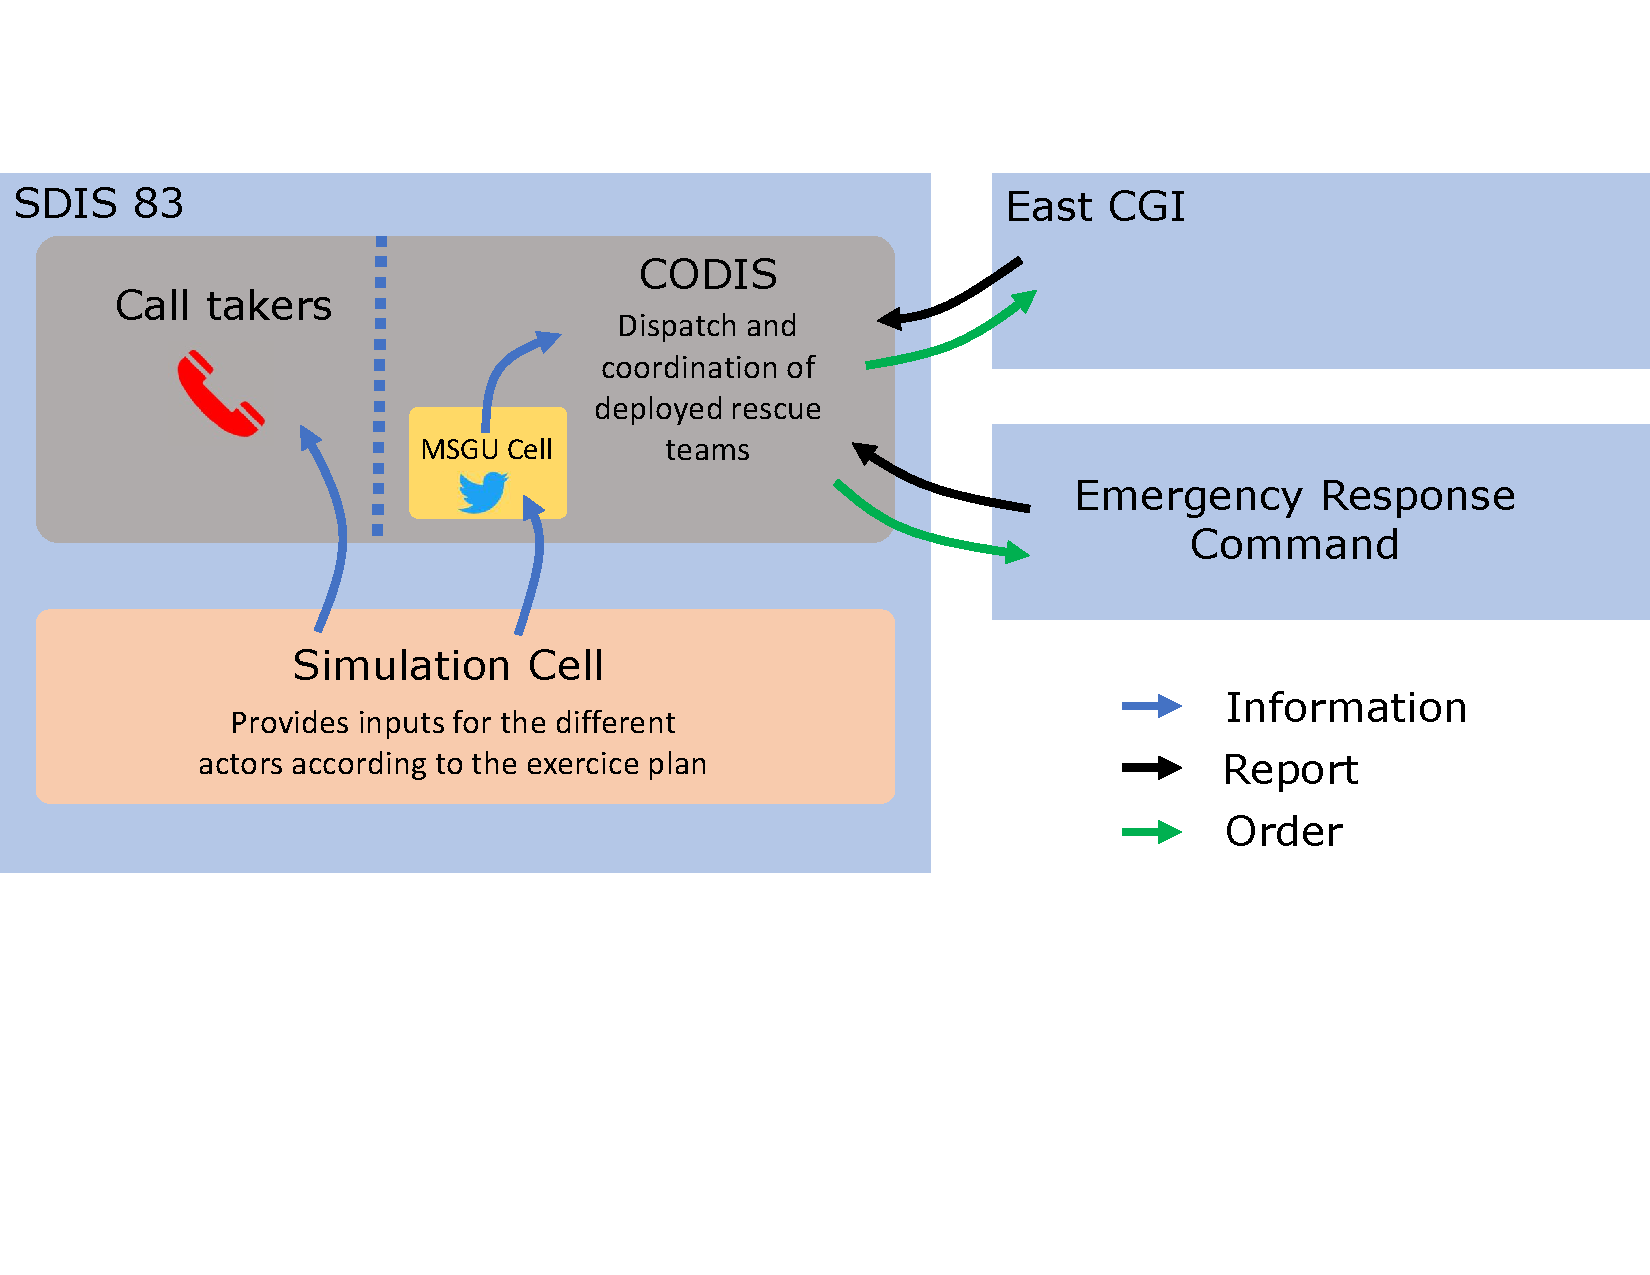
\includegraphics[width=\textwidth]{figures/chap-3/SDIS83.pdf}
    \caption{Organizational diagram of Exercise 1 MACIV at SDIS83 in the Var Department.}
    \label{information:sdis83}
\end{figure}

The profil of this operator was one of a volunteer firefighter, who is familiar with social media and communication.
This operator was in charge of monitoring social media and cross-referencing the information they could obtain with that provided by VISOV the Volontaires Internationaux en Soutien Opérationnel Virtuel (VISOV, french equivalent of the \textit{Virtual Operations Support Teams} — VOST) association.
The VISOV association is mostly composed of volunteers with a background in public service, rescue operations etc.
These volunteers monitor social media on their free time to identify information related to a potential, or already ongoing event.
They regroup their findings in a live Google Sheet~\footnote{https://www.google.fr/intl/fr/sheets/about/} document.
A Google Sheet document is a tabular file, identic to an Excel file, where multiple persons can modify simultaneously the document and see the changes in real time.
This live document is then shared with the person in charge of social media processing within official institutions.
Using there own findings and the ones from the online document, the MSGU operator will then provide the information obtained when asked by the decision maker in the room.

In the second and third exercise, the institutions were mostly relying on the processing realized by the VISOV association.
The setting of these exercises is illustrated in Figure~\ref{information:exercise-prefecture}
The operators in charge of the social media in the préfectures were persons from the communication team of each préfecture.
In this case, these persons were not familiar with emergency or rescue operations.
They were mostly tasked with communication to the public using the official accounts of the institution they were part of.
Monitoring of social media activity and information gathering were not the priorities of these operators.
The precise sequence of these exercises and their context is detailed in \textcite{batardIntegrerContributionsCitoyennes2021}.

\begin{figure}[htb]
    \centering
    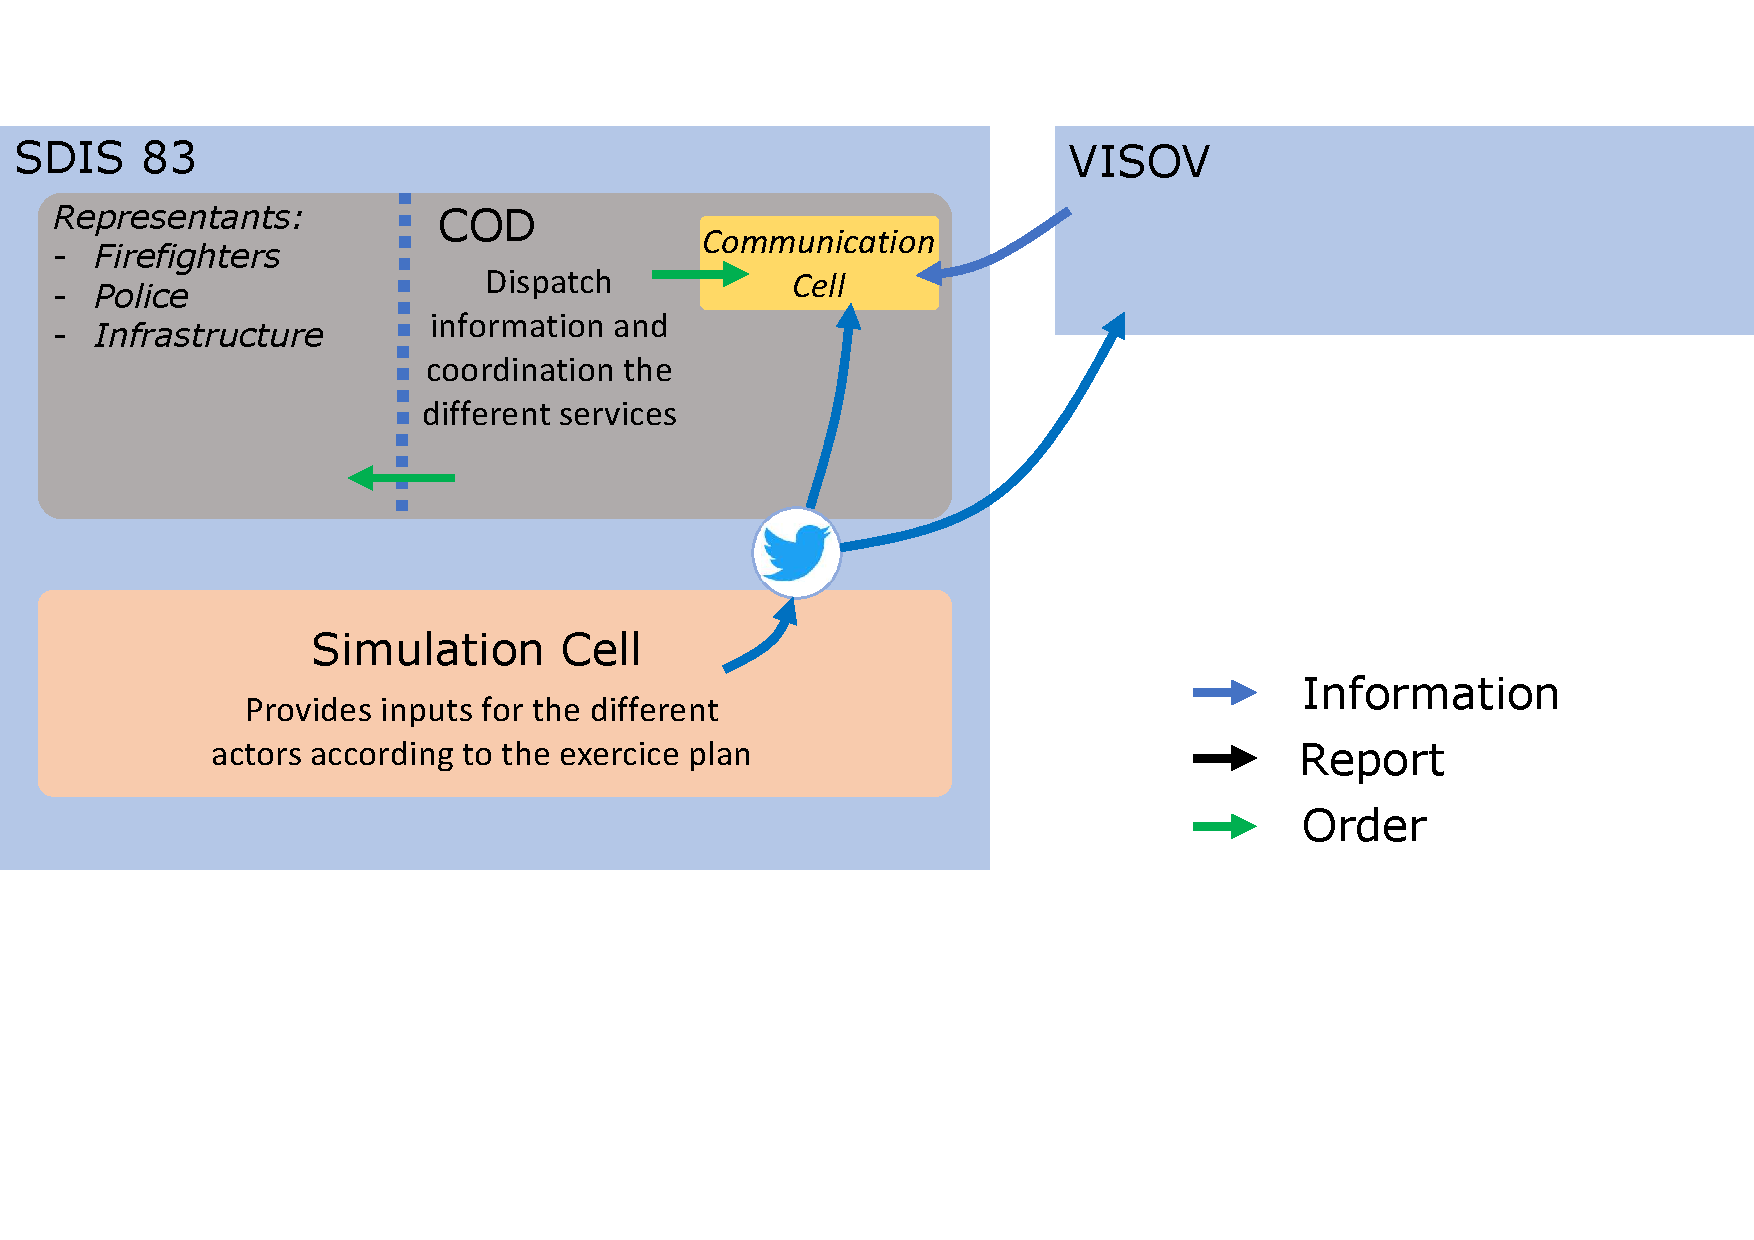
\includegraphics[width=\textwidth]{figures/chap-3/prefectures.pdf}
    \caption{Organizational diagram of Exercises 2 \& 3 MACIV in the different Préfectures involved.}
    \label{information:exercise-prefecture}
\end{figure}

The depth of the exercises allows to witness a more significant part of the information within the organization.
The different institutions use a software similar to the CAD software used in the U.S. to share information.
This information system is called SYNERGI (SYstème Numérique d’Échange, de Remontée et de Gestion des Informations).
Similarly to the CAD system, this system has some criticisms.
\textcite{linotPerspectiveComputationnelleDefi2018} report that the user suffers from:

\begin{itemize}
    \item Its rigidity, which leads to system circumvention;
    \item Communication issues, caused by a lack of common vocabulary;
    \item The diversity of unprepared institutions involved, leading to poor coordination;
    \item Lack of context associated with the information shared, adding confusion.
\end{itemize}

Figure~\ref{information:french-orga} illustrates the organization of the institutions and the flow of information between them.
However, where the CAD system allows for coordination between call takers and dispatchers
through a common interface, the scale and official status of the SYNERGI system prevent the share of information coming from social media on this platform.
Also, it is interesting to note the particular status of social media data within this information pipeline.
\textcite{castagninoWhatCanWe2019} highlights the segregation of social media, systematically assumed as an untrustworthy information during the first exercise.
This behavior was also witnessed during the two other exercises.

\begin{figure}[htb]
    \centering
    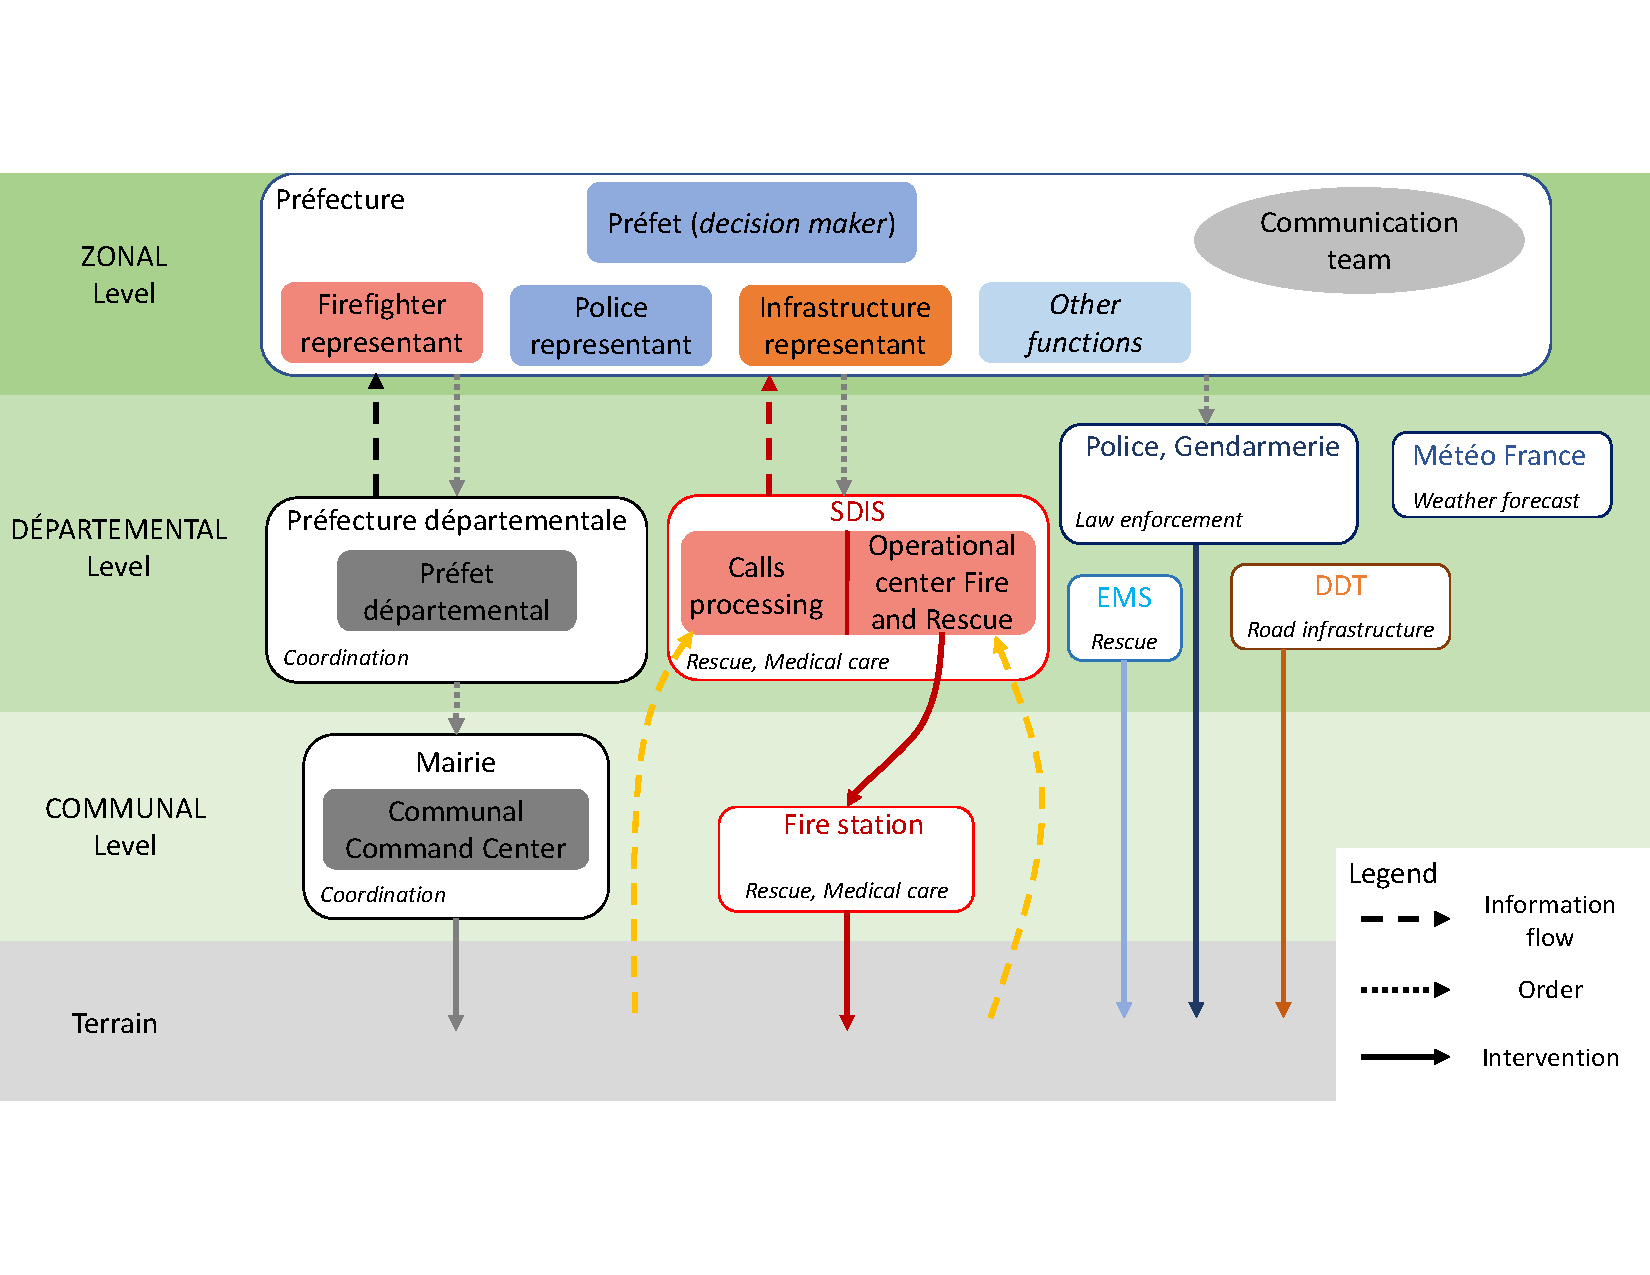
\includegraphics[width=\textwidth]{figures/chap-3/french-orga.pdf}
    \caption{Diagram of the organization of the different French institutions involved during the response to an event of zonal scale.}
    \label{information:french-orga}
\end{figure}

There are a wide variety of PSAP configurations in the U.S., but the one I observed was composed of 2 centers:
1 for calls and 1 for allocating resources to the various events.
When the role of operator assigned to the social media is considered, it is placed alongside the call takers.
The two roles are indeed thought in a similar way.
In centers with fewer resources and where operators are responsible for both call taking and dispatch,
social media is seen as another channel that would be monitored in a mostly passive way.
In France, media operators can be found at different levels in the hierarchy of response actors.
For the time being, this distribution depends on the interest that each one has in social media.
In the case of the first exercise, the SDIS had a dedicated operator alongside their call taker
and were cross-checking information.
In the other two exercises, it was the communication cell of the Prefectures that was
monitoring social media, to provide information to the decision makers.
In all French cases, their operators were assisted by a third-party of volunteers, VISOV.
Looking back, the overall structure of the organization is very similar in both countries.
It is mainly operators, who monitor social media themselves, or
assisted by a third party entity \parencite{batardIntegrerContributionsCitoyennes2021}.
These operators then feed the information back to the decision-makers.
The profile of the operators is very diverse, but in the situation encountered, they
were either communicants or staff used to handle calls.
French organizations studied felt overall more suspicious of information coming from
social media \parencite{castagninoWhatCanWe2019} than their American counterparts.
Lastly, it is reasonable to assume that both countries are at the same stage of consideration, i.e., early adoption

\section{Information needs identified}
It appears that in the majority of cases, the information coming from social media passes through at least one intermediary before reaching the decision maker.
Decision makers need information, but they are not the persons actively monitoring social media.
Thus, the staff responsible for retrieving information from social media must therefore orient their research towards the needs of decision makers.
Several questions therefore arise:

\begin{itemize}
    \item What information do decision makers need?
    \item What information are the operators looking to retrieve?
\end{itemize}

The first question is what is driving the whole system.
The decision makers' needs have to be answered, and this is the role of the support operators (call takers and social media operators) to fulfill these needs.
The second question looks at the information that operators search for in the stream of social media messages.
This question guides the development of the algorithms responsible for the retrieval of data presented in the next chapter.
The remainder of this section develops the analysis of this need in light of previous work that
has defined concepts such as situational awareness and actionable information.

\subsection{Situational awareness}
Situational awareness is often described in simple terms as the understanding of the "big picture" of the situation.
More precisely, it is the comprehension of the different aspects of an event, environment, and/or entities and how they are more likely to evolve in the near future.
Sufficient situational awareness is a critical factor in decision making.
Each individual has its own situational awareness, depending on several factors such as experience, perception ability, training etc.
The group formed by individuals also carries its own situational awareness.
As described in Chapter 1, emergency situations are confusing events that reset situational awareness.
The decision-makers in charge of the response must therefore build an updated mental representation of their environment.
This task is all the more difficult as the context is unstable and may continue to evolve as a result of aftershocks or cascade effects.
In addition, the amount of new information can be overwhelming, depending on the size or complexity of the event.
In the described context, it appears crucial that decision makers rely on adapted methodologies and tools to reconstruct adequate situational awareness for decision making.
This work and definition attracted the interest of the U.S. military, who embraced the concept, working permanently in a stressful and highly uncertain environment.
\textcite{departmentofthearmyAdvancedSituationalAwareness2021} compiles the doctrine they have built around the concept, including how it fits into the decision-making process and how situational awareness is influenced by the environment.

The currently dominant definition is seminal work presented in \parencite{endsleyTheorySituationAwareness1995}.
\citeauthor{endsleyTheorySituationAwareness1995}, propose a definition of situational awareness as well as a model to explain how it fits into the decision-making process.
They define situational awareness as the "perception of the elements in the environment within a volume of time and space, the comprehension of their meaning and the projection of their status in the near future" \parencite[p. 36]{kropczynskiIdentifyingActionableInformation2018}.
This definition is associated with three levels: (1) perception, (2) comprehension, and (3) projection.
Perception refers to an operator's ability to detect relevant signals through the senses.
Level 2, comprehension, refers to the ability to interpret and make connections between perceived signals.
The last level, level 3, corresponds to the ability to anticipate future events based on available information.
Figure~\ref{information:SA} provides an overview of situational awareness in the decision-making process according to \parencite{endsleyTheorySituationAwareness1995}.

\begin{figure}
    \centering
    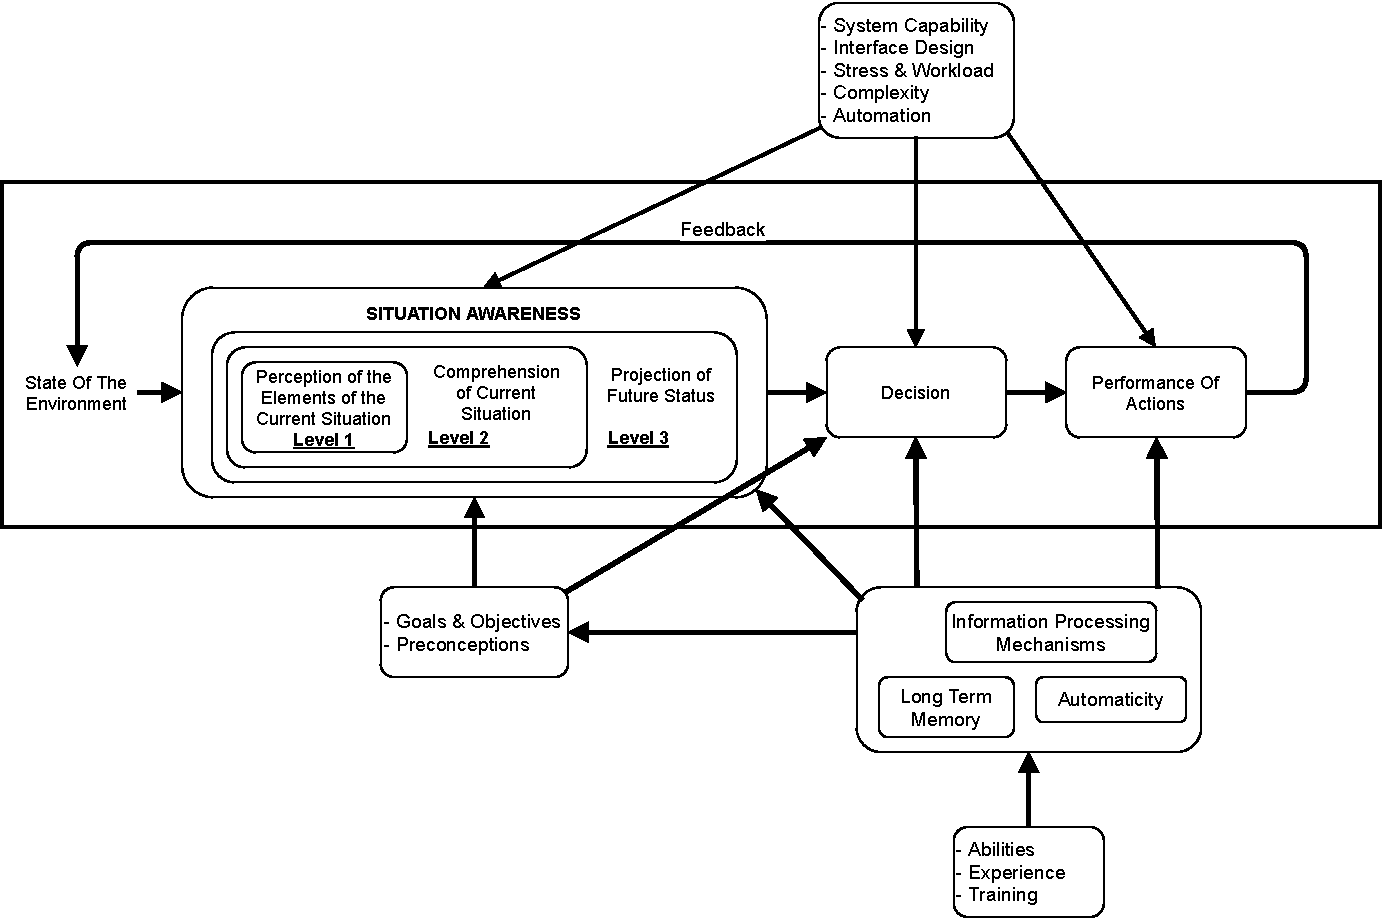
\includegraphics[width=\textwidth]{figures/chap-3/Endsley-1995.pdf}
    \caption{Situational awareness model from \textcite{endsleyTheorySituationAwareness1995}.}
    \label{information:SA}
\end{figure}

Numerous works in crisis informatics have extended this definition to meet the needs of this domain.
\textcite{viewegSituationalAwarenessMass2012} thus uses the definition of \textcite{endsleyTheorySituationAwareness1995} in that it tries to identify if the content of microblog contents can be useful during massive emergencies.
The author therefore starts from a corpus of messages posted on Twitter during different events and identifies tweets that have the potential to improve situational awareness.

Later, \textcite{vermaNaturalLanguageProcessing2011} proposed to automate the processing of this information by natural language processing systems.
Inspired by this proposition, several research teams built software to reproduce the results of \citeauthor{viewegSituationalAwarenessMass2012} using computational automation.
These systems aim to improve the user's situational awareness during mass emergencies.
Many systems have been developed to classify tweets \parencite{carageaClassifyingTextMessages2011, imranAIDRArtificialIntelligence2014,ashktorabTweedrMiningTwitter2014}.
More recently, systems proposing a multi-modal approach (image + text) have been proposed.
The multiplication of heterogeneous data collection channels is a promising approach.
This approach enables systems to bring different points of view on the same event to the user.
It also brings an interesting research perspective, especially when it comes to merging the two types of data.
The combination of heterogeneous data sources can provide opportunities:

\begin{enumerate}
    \item Collect more information,
    \item Verify certain information when text and image overlap, and
    \item Fill gaps in one information source with that of another.
\end{enumerate}

Specifically, \textcite{jacksonInformationSharingEmergency2006} present four types of information that support situational awareness to protect emergency responders.
These four types of information are:

\begin{enumerate}
    \item Information about the hazard environment
    \item Information on the responder workforce
    \item Information on evolving safety issues
    \item Information about safety equipment
\end{enumerate}

These points are reused later by \textcite{yangDesignPrinciplesIntegrated2012}, that generalized these points, and, more anecdotally, correspond to information that was requested by the decision-makers during the exercises I observed.
This information allows decision makers to make crisis response decisions while protecting their teams.
These four needs can also be generalized, as discussed at the end of the next sub-section.

Improving situational awareness is a common goal of many social media data aggregation systems and are espoused to address information needs first responders.
Much progress has been made on data aggregation, processing, and analysis thanks to the work of these teams.
However, given that these systems are not often utilized by practitioners, we believe that enhanced situational awareness alone is unsatisfactory.
Instead, evidence pointing to the need to consider other aspects of the information processing pipeline bears consideration in the development of new data systems.

\subsection{Actionable information}
As previously mentioned, fieldwork with crisis managers and operators of call centers found
that situational awareness was not the only information need expressed by the practitioners
\parencite{zadeSituationalAwarenessActionability2018, kropczynskiIdentifyingActionableInformation2018}.
Depending on the nature of the incident, a crisis management team can find themselves lacking
the critical information to take action, or on the contrary, be overloaded with information.
This leads to a situation of paralysis of the decision makers, despite the fact that they have the necessary information.
The interviewees therefore refer to the need for actionable information, i.e., information that enables decision-making.
Thus, as systems that process social media data act as an additional source of information, they can fuel information overload.
Hence, the proper design of these systems is of utmost importance (see Chapter 5).
The rest of this section focuses on this concept, its definition and what it implies for the processing of social media data.

Actionable information can then be considered as a specific type of information.
\textcite{yangDesignPrinciplesIntegrated2012} indicate that the fire response system should focus on information that is (i) timely, (ii) accurate, and (iii) complete.
For instance, information that provide the exact location of the event (accurate information) and the environmental conditions (complete information).
\textcite{comesBringingStructureDisaster2015} call for a similar set of attributes to define the information needed in an information system for crisis response: (i) relevant, (ii) accurate, (iii) timely.
\textcite{zadeSituationalAwarenessActionability2018} conducted a survey and various interviews of emergency and humanitarian responders.
They focused their research on the question "how can the right information reach the right person at the right time?"
In their approach to this research, they first asked practitioners to define actionability.
\textcite{zadeSituationalAwarenessActionability2018} report "participants described actionable
information as anything which either they or their organization could use at that moment to assist,
enact, or expedite the solution to a (potentially) identified issue."
More importantly, the authors report that the practitioners were using a definition according to their organizational role.
To summarize, \citeauthor{zadeSituationalAwarenessActionability2018} identified the same
attributes as previously, with an emphasize that the actionable property of an information
also depends on the role of the person that receive the information (e.g. an information
can be actionable for a firefighter, but not for EMS).
They add credibility of the information.
As a result of all the point of views presented, an information is actionable if it is:

\begin{itemize}
    \item Located
    \item Addressed to the right role
    \item Timely
    \item Credible
    \item Provides context
\end{itemize}

An actionable information must meet the information needs of decision makers (it provides context).
This information has been credible enough (the information comes with additional proofs or is provided by a trustworthy source).
This information can be sufficiently localized to allow the deployment of resources.
Finally, the information is addressed to the right person, at the right time.
\textit{Accuracy} and \textit{relevance} are removed from the list as they are too generic.
In reality, it is rare to see information that meets all the above criteria.
In the case of Twitter's content, this piece of information is referred as a "golden tweet" \parencite{kropczynskiIdentifyingActionableInformation2018}.
During interviews with American emergency call centers' operators, \textcite{kropczynskiIdentifyingActionableInformation2018}
try to capture the process used by call takers to capture actionable information through calls.
For this purpose, 911 operators use Six W's.
These Six W's are: \textit{Where} is the assistance needed, \textit{What} is the event taking place,
\textit{Weapon(s)} involved in the event (if relevant to the nature of the event),
\textit{Who} is involved in the event, \textit{When} the event started,
and in some cases information is collected regarding \textit{Why} the event is happening.
These specific questions help the call takers to acquire specific information that were
identified has the most useful information to respond quickly and effectively an emergency—
or in other words, to take action with regard to a particular event.
The goal of the Six W's is to obtain information that match the information needs of the decision makers requirements and consequently to provide actionable information to the dispatchers and responding teams.
Each W asked effectively match the actionable information criteria proposed above.
The \textit{Where} question is especially salient, and was mentioned as the most important question.
It is indeed the piece of information that dispatchers will then use to send resources at the location of the event.
All the other questions provide additional context.
Later, \citeauthor{kropczynskiIdentifyingActionableInformation2018} refined the coding scheme they obtained with subcategories.
To do so, they conducted an analysis of a corpus of tweets to determine how actionable information appears within actual social media posts during a crisis \parencite{kropczynskiRefiningCodingScheme2019}.
At the light of this refined ontology, they coded 200 tweets and reported the proportion of tweets that were fitting in these categories.
Their results show that among the tweets, four of the categories (Where, What, Who, Why) were significantly present, while two (Weapon and When) were rare.
With social media content, the Six W's might process is then slightly modified.
Usually, there is no follow up information to fill the missing attributes like in a regular phone call.
A social media processing therefore have to consider that specificity.
It can be address by aggregating the pieces of information retrieved from both call takers and social media operators within a unified system.

\subsection{Information needs of a crisis management organization}
The information needs of decision-makers depend on the crisis at hand.
However, from the results of the above-mentioned observations, one can identify patterns
that would be common in most of the situations faced and that are crucial to the decision-making process.
The decision makers express several needs.
First, they need constant and specific information (what is the emergency? where is the emergency? ...)
This information is obvious for crisis management and as such, is barely mentioned in the
interviews, which are often oriented towards identifying less visible needs.
The information sought through the Six W's and the information needed exposed by \textcite{jacksonInformationSharingEmergency2006}
compose what would be the "baseline" information needs.
These are:

\begin{enumerate}
    \item Location of event, type, cause and severity;
    \item Environmental conditions (buildings, population density, potential hazards and their location...);
    \item Information on the response participants (responders already involved, their skills, resources...);
    \item Current and future needs of the responders (number of casualties, their status...); and
    \item The available resources to the event (qualified actors, appropriate equipment...)
\end{enumerate}

In addition to these basic information needs, when asked, emergency management organizations
request "actionable information".
An actionable information is a piece, or the last missing piece, of information which enables
immediate decision making.
Actionable information can be seen as a "super information", i.e., an information with additional properties.
It is an information that:

\begin{itemize}
    \item is located;
    \item is directed to the right role;
    \item is timely;
    \item is credible;
    \item provides context.
\end{itemize}

The different attributes are ordered by importance.
A response can be triggered if the decision maker (or the dispatcher) can understand the emergency
and know where to allocate resources.
But crisis management often involve multiple, distributed actors that are not necessarily
used to work together.
Thus, it is not uncommon for one of the actors to have information that is of little interest to him,
but which turns out to be critical for another actor.
The timing of this information is important, as an information that arrives too late can be rendered useless.
Having an information coming from a trustworthy source is also an advantage.
The crisis managers I met with and asked about credibility said that in the case of a message
mentioning an emergency and whose source is not trustworthy, they send a team to recon.
During the first exercise of the MACIV project,  social media messages sent by ordinary
citizens and whose veracity they could not confirm were processed this way by the emergency managers.
The "additional context" criteria correspond to the other pieces of information required
by decision makers to respond effectively to the event.
While credibility, context and the mention of a location of information are properties of
the information, the criteria of "right person at the right time" criteria are more linked
to the organization in charge of the response.

In this view, an actionable information is an information that matches several criteria
that would lead a decision maker to makes a decision and send resources.
Actionable information is the trigger of the resource allocation.
However, proper response, that would lead to the resolution of the event, requires additional
information.
It is information that is latent to the situation (hazards, deployed and available resources, victims etc.).
These additional pieces of information are part of the "context" of the crisis (resources available,
responders already deployed etc.).
This information constitutes, as explained above, the decision maker's situational awareness.

Figure~\ref{information:sa-inf} summarizes the link between situational awareness and actionable information.

\begin{figure}
    \centering
    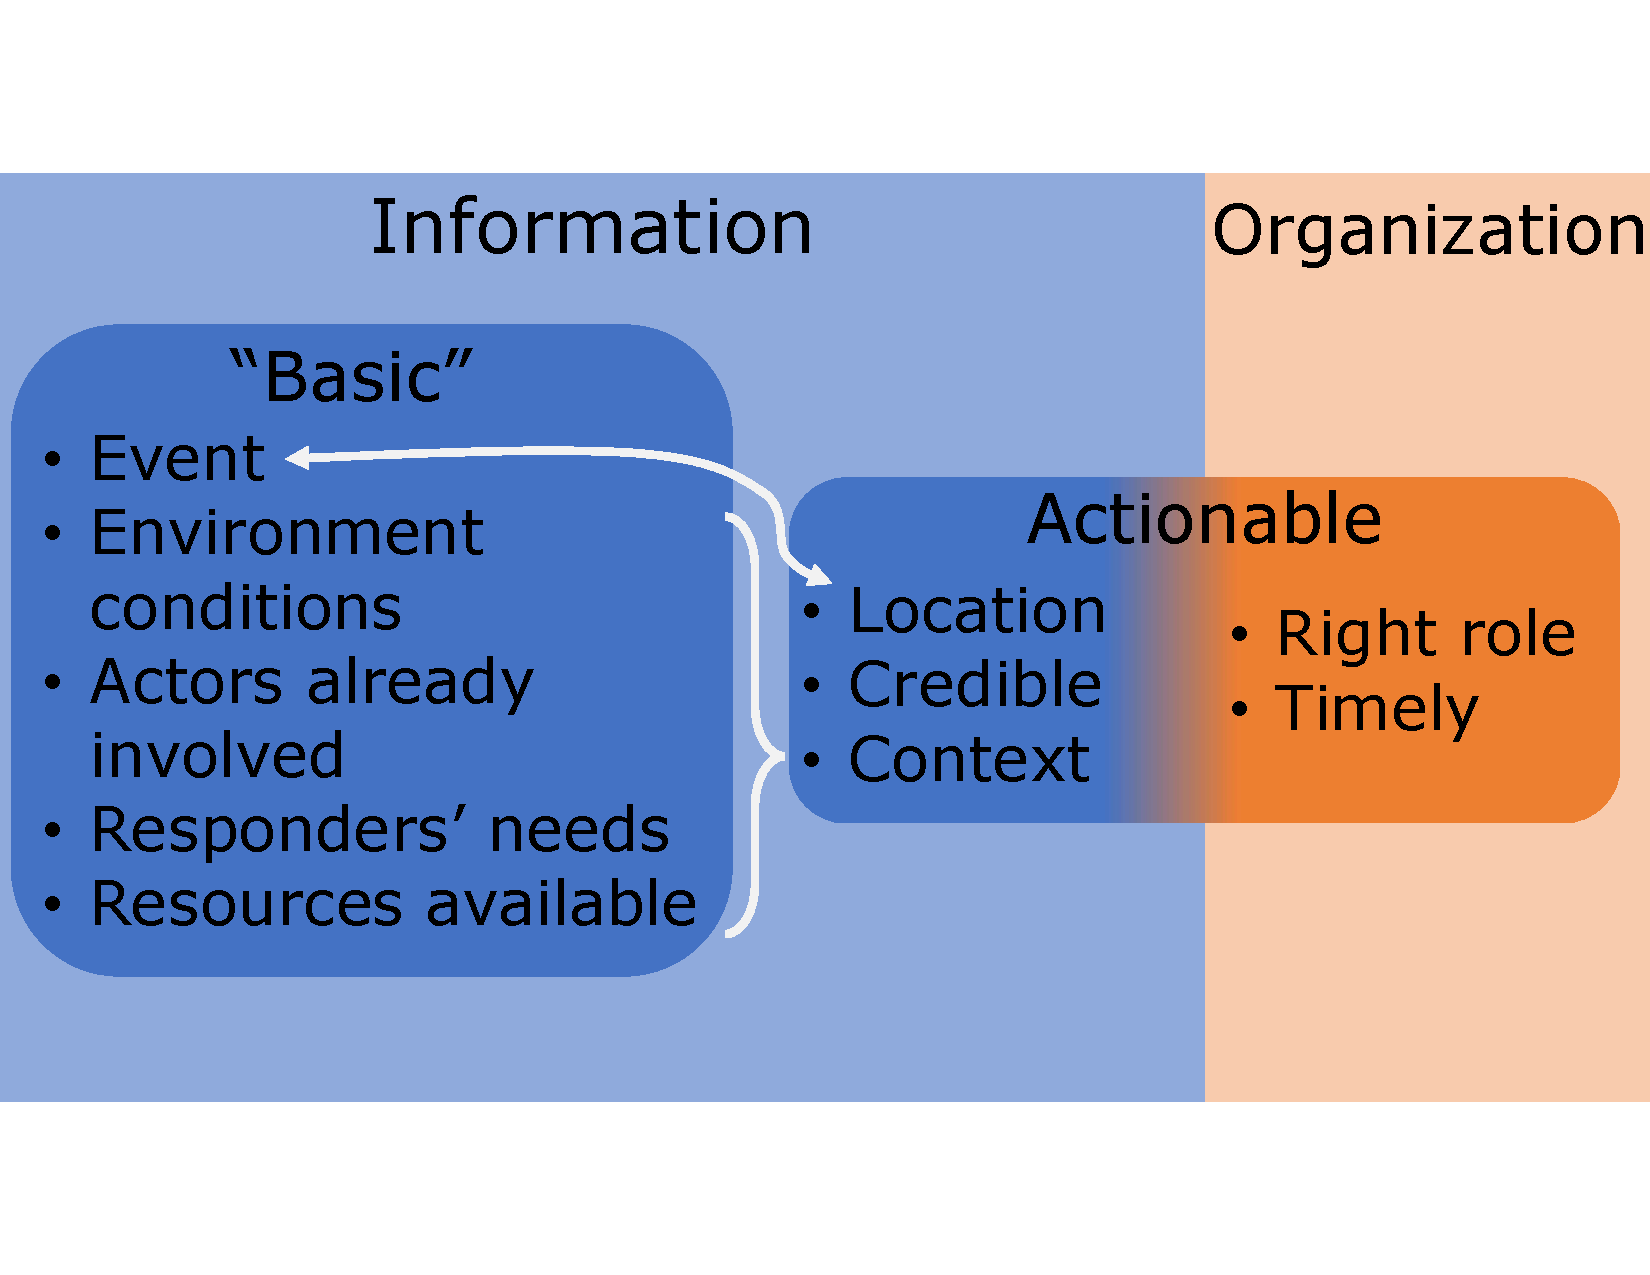
\includegraphics[width=\textwidth]{figures/chap-3/sa-ainf.pdf}
    \caption{Shared attributes between elemental information needs for crisis response and criteria for an information to be actionable.}
    \label{information:sa-inf}
\end{figure}

\subsection*{Summary}
This section sought to answer two questions:

\begin{itemize}
    \item What information do decision makers need?
    \item What information are the operators looking to retrieve?
\end{itemize}

Call takers and social media operators are looking for information that meet minimal requirements.
However, an information that meet one of these requirements, provide a location and that is delivered
to the right person, at the right time, is described as an actionable information.
Actionable information is requested by crisis management organizations, as they are information that
facilitate decision making and therefore provide greater results.
In real world situation, it is very challenging and rare to have information that corresponds to all criteria simultaneously.
Social media, as others information channel cannot provide alone actionable information.
On the other hand, social media can provide pieces of information that improve the situation
awareness of the decision makers by adding elements to the context.
This additional context can then, on some occasions, provide actionable information.
However, this capacity can only be unlocked by creating a direct and collaborative means
of communication between the operators responsible for monitoring the different information channels.
This information system calls for an ontology, or information model, that is able to take
into account information from both channels.
The aim of the next section is to define this abstraction in the light of the elements
presented so far.

\section{Crisis information models informed with situational awareness}
As presented in the first chapter, the crisis response phase requires the deployment of resources that are very quickly stretched.
Moreover, an adequate and efficient response cannot be put in place without prior information.
The automation of the collection and support of information processing is therefore a considerable advantage in a crisis situation.
However, such a capability requires an information model capable of representing the information that responders need \parencite{comesBringingStructureDisaster2015}.
The first sub-section attempts to integrate actionable information into the model used to describe situational awareness.
The objective of this sub-section is to consider how the notion of actionable information can support the construction of an information model for crisis response.
The second sub-section presents an information model for the response.

\subsection{Location of actionable information in the situational awareness model.}
Situational awareness is the initial building block of decision making in crisis response.
An information cannot be designated as actionable without the decision maker having sufficient context to decide if that information is actionable.
Therefore, crisis management starts by recovering an adequate perception of the elements/assets of the environment (level 1 of SA).
From that perception, they will use their skills/training to understand (level 2 of SA) the current situation.
Then, decision makers evaluate the future status of their environment (level 3 of SA).
In this picture, an actionable information is an information that can immediately triggers a decision from the decision-makers.
For instance, a social media operator receives a report of an injured person.
The decisions makers would need to know the location of the victim and which type of equipment is required.
However, if they don't know the status of their evacuation resources or a safe zone to evacuate,
due to the disruption created by the event, they might prefer to not consider this piece of information as actionable.
While it is a useful and important piece of information, decision makers have to delay their final decision on the evacuation.
In this case, they would prefer to recover a better situation awareness
Only when they will have a sufficient perception of their environment they will be able to order the evacuation of the injured person.

Both the concept of Actionable Information and Situational Awareness are then linked to the concept of Information.
Here, we use the definitions of Data and Information proposed by \textcite{ackoffDataWisdom1989} in his Data-Information-Knowledge-Wisdom framework.
The concept of Data is an abstraction.
It refers to symbols that have no meaning beyond their existence.
Information on the other hand, is data that has been given meaning by the creation of connections between those points.
Information generally answers questions such as "who", "what", "where" and "when".
Thus, the caller takers interviewed in \textcite{kropczynskiIdentifyingActionableInformation2018} are gathering Information through the Six W's.

Information and Data are also present in the Situational Awareness model proposed in \textcite{endsleyTheorySituationAwareness1995}.
To the three levels proposed, and described earlier in the literature review, we can associate the Data-Information-Knowledge concepts as proposed in Figure~\ref{information:SA-DIK}.

\begin{figure}
    \centering
    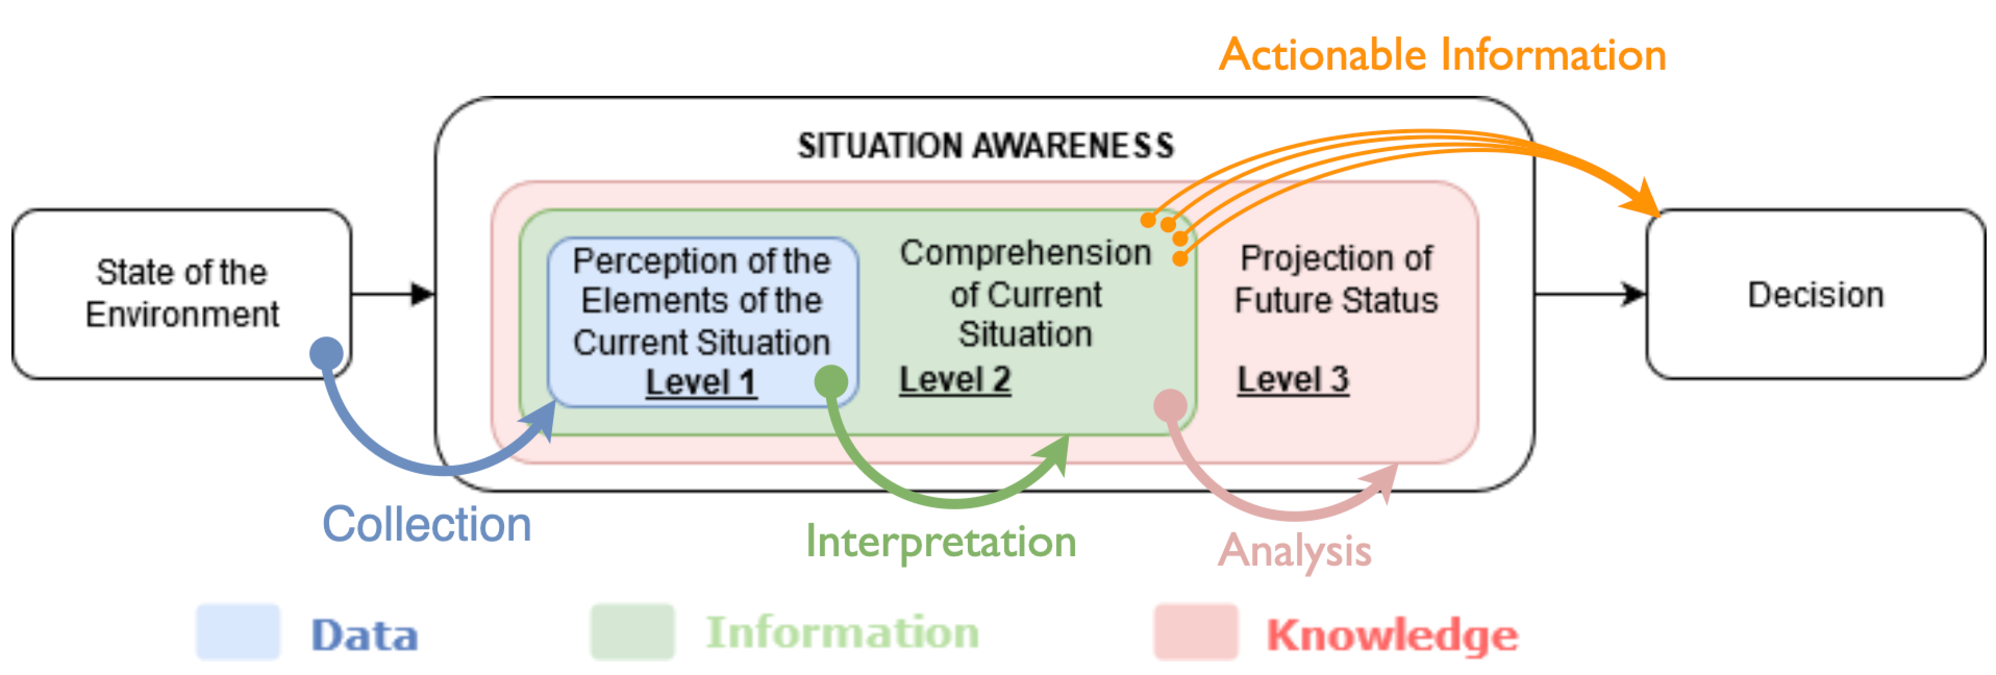
\includegraphics[width=\textwidth]{figures/chap-3/Fig2-2.pdf}
    \caption{Location of Data-Information-Knowledge concepts in the Situational Awareness model}
    \label{information:SA-DIK}
\end{figure}

The first level of Situational awareness concerns the perception of the "elements/assets" (or data) of the environment.
Effective data collection allows a decision-maker to achieve a sufficient perception of the surrounding environment and a means to describe it.
Assuming this first level is effective, the second level of Situational Awareness consists of being able to form patterns with the other elements/assets.
Through the interpretation of the different data points and the way they interact with each other, the operator is able to understand the ongoing situation.
This is this level of Situational Awareness that decision-makers are required to reach to be able to make decision.
This is also this same level that is often lost during the chaotic nature of a mass emergency event, and that decision makers try to recover using situational awareness tools \parencite{endsleyTheorySituationAwareness1995}.
The final level uses the patterns known or identified by the decision-makers to make predictions on the future states of the environment, thus referring to the Knowledge layer of the framework.
It is preferred that the decision-maker has this level of Situational Awareness, but it is not necessarily required.

Situational Awareness is built upon any Data or Information about the current state of environment and that is delivered to the decision-maker.
Using the previous proposition, we are now able to envision a relationship between Situational Awareness and Actionable Information.
As Actionable Information is a type of Information, it is then embedded in the second level of Situational Awareness.
The difference with regular Information, is that Actionable Information is the missing piece of the puzzle that allows the decision-makers to decide.
As a result, Situational Awareness is the puzzle comprised of pieces of Information that
decision makers try to assemble during the event, and Actionable Information constitutes
the final, missing pieces of that puzzle necessary to comprehend the whole.
Actionable Information is then a specific piece of Information in the Situational Awareness model.

All these criteria are context dependent.
As an example, when is an information delivered "at the right time"?
The right time can be seen as a time window allowed by the acquisition of previous incomplete
information, with missing parts and where a new incoming information complete the puzzle.
Timeliness, credibility and adequacy of the role, as subjective criteria, are mostly context dependent.
It is therefore very difficult to set a threshold for these values that would "simply" collect Actionable Information.
\textcite{silberschatzWhatMakesPatterns1996} describe two major issues with the processing of Actionable Information:
(i) there are a lot of patterns of interest, that have to be divided into a finite set of action-pattern equivalence;
(ii) pattern-action associations are likely to change overtime, thus, the life cycle of these associations has to be managed.
The concept of actionable information is important, yet and fuzzy and context-dependant, as the criteria above show.

\subsection{Implications for Social Media Processing System Design}
As \textcite{zadeSituationalAwarenessActionability2018} highlighted, proposed social media systems have not been widely adopted by emergency responders.
Among all the reasons that could explain this lack of interest, some are certainly related to the design of the systems.
Systems initially developed were focused on increasing the amount of information provided to first responders.
However, the misfit of the categories used by these classification systems ultimately lead to adding noise in the processing.
In addition, the information did not always fit the responder's need, resulting in additional noise.
Current systems handle data collection and information extraction.
But the resulting flow might still be overwhelming for social media operators.
The systems developed should require a minimal amount of attention from the operators on the menial tasks, while keeping her engaged.
As the goal of increasing the volume of information available to emergency managers can be considered as achieved, future work could concern information quality.
This quality improvement can be achieved by adding support to Actionable Information identification.
But, as stated earlier, Actionable Information can be identified by systems only by having a sufficient Situational Awareness at first hand.
Thus, social media processing systems need to be able to both perceive and comprehend the situation.
Also, initially difficult to focus an information system on the concept of Actionable Information,
because it is very challenging to define clearly "the right person at the right time".
The criteria of location, contextualization and credibility of the information already offer more opportunities from an information system perspective.
An information system to support social media operators in crisis response is therefore more centered around situational awareness.
Thus, it considers the two types of actors that interact with the model.
The model must meet the needs of both actors and in particular not hinder their workflow.
Call takers must be able to submit the information they consider relevant.
Decision makers must be able to quickly identify the information they need during the response.

All these considerations lead to the information model summarized in Figure~\ref{information:information-models}

\begin{figure}
    \centering
    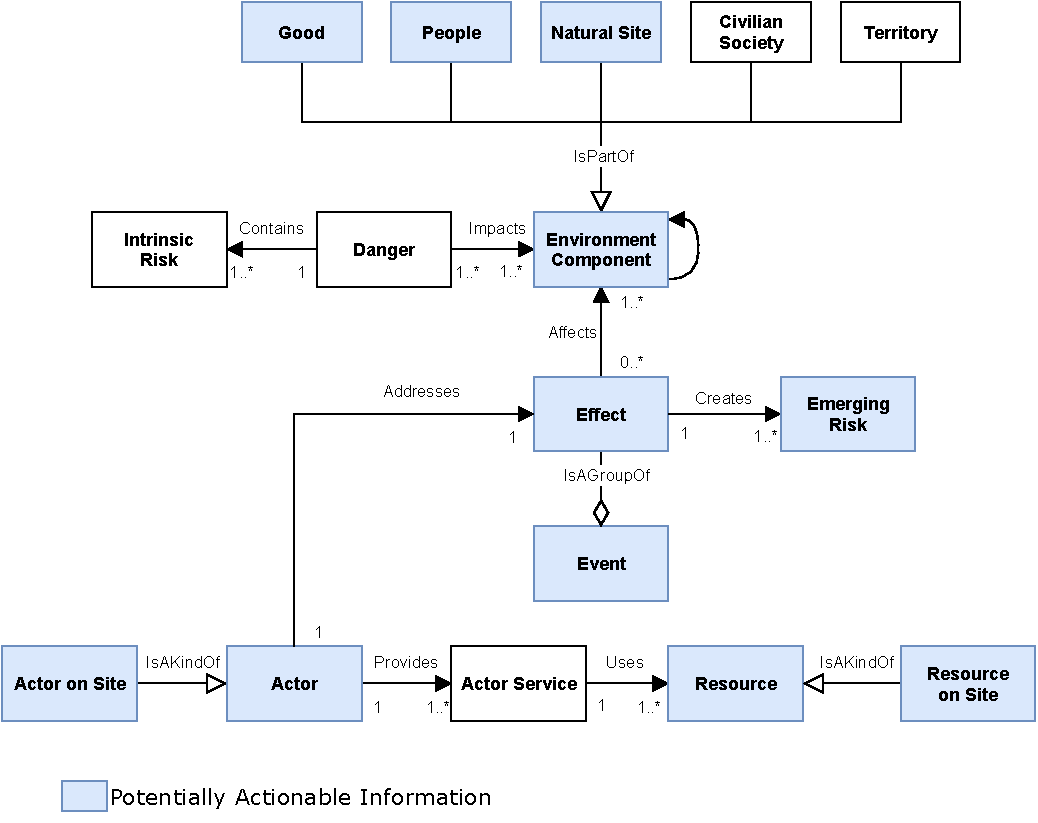
\includegraphics[width=\textwidth]{figures/chap-3/information-needs.pdf}
    \caption{Proposed information models, produced after reviewing the information handled the call takers and needed by decision makers.}
    \label{information:information-models}
\end{figure}

The model is composed of nine entities:
\begin{itemize}
    \item Event
    \item Environment
    \item Actors involved
    \item Responders needs
    \item Resources available
    \item Location
    \item Hazard
    \item Equipment
    \item Actors
\end{itemize}

It is centered around the concept of Event.
Several attributes allow the call takers/social media operators to describe an event such as
the Location, the type, the severity, or the cause.
The Location of an event can be a specific address, the name of a place or a generic one,
such as a neighborhood, an indication of a city blocks etc.
The Event entity is linked to four other entities that are responsible for informing the event.
These entities are Environment, Actors involved, Responders needs and Resources available.

An Event takes place in an Environment.
An environment can have a population density, hazards or indications provided by the callers.
There may also be different types of hazards, which may or may not be localized.
An environment can host several events, possess multiple hazards, see multiple actors involved
that have different needs.
Hence, entities that describe who are involved in an event (Actors involved) that describe the
Actors involved and their Equipment.
The actors have different skills, like firemen or policemen in the case of professionals.
However, there may also be civilian actors who may or may not have skills.
A similar reasoning is applied to Equipment, which are often used in the fight against specific hazards.
The Actors involved have (or are going to have needs) according to the type of event and the
specificities of the environment.
In order to fight an event and address hazards, responders have access to Resources Available.
The resources are composed of actors or equipments that are not engaged in an action.

The proposed information model is reused throughout the rest of the manuscript.
Chapter 4 presents an algorithm that aims at automatically detecting previous entities in messages.
Chapter 5 proposes an architecture for the above-mentioned information system, which is built around the entities described in this chapter.

\section{Conclusion}
This chapter explores the information needs of decision-makers during crisis response and
proposes an information model to build an information system to support crisis management organizations.
As a reminder, the needs retained are:

\begin{enumerate}
    \item Event (location, type, cause and severity);
    \item Environmental conditions (buildings, population density, potential hazards and their location...);
    \item Information on the response participants (responders already involved, their skills, resources...);
    \item Current and future needs of the responders (number of casualties, their status...); and
    \item Resources available for the response (qualified actors, appropriate equipment...)
\end{enumerate}

This section discussed two concepts widely used in the crisis management community: situational awareness and actionable information.
We have taken the definition of these two concepts and developed how they can be adapted to the content available on social media.
In particular, we have seen that in practice, response teams are primarily looking for actionable information.
However, the individual data available on social media very rarely meets all the criteria that would allow them to define their information as actionable.
to define their information as actionable.
If relevant information posted on social media is rare, golden tweets are even rarer.
However, if we go back to the concept of situational awareness, we understand that actionable information is not an entity living in a vacuum in the middle of the crisis.
Actionable information is in fact extremely linked to its context and lives only in it.
This underlines the importance, as a decision-maker, of having the best possible overview of the situation, in order to determine
whether a piece of information is actionable, or to which other actor it might be.
For social media operators, in charge of content processing, it is (I think) illusory to find actionable information as it is in social media.
On the contrary, they should expect to find pieces of information that, similar to
similar to puzzle pieces, lead to actionable information once assembled.

As a final note, decision makers need actionable information to make decisions.
The role of the social media operator is to look for bits and pieces of information, which when aggregated can provide actionable information.
Not all data has to come from social media alone.
As mentioned earlier, \textcite{graceRolePlayingNext2019} emphasize the importance of
maintaining a similar information processing protocol between call takers and social media
operators, in order to maintain the existing fluidity.
This calls for a tool capable of bridging the gap between the two mediums, based on
abstraction that crosses the information needs of decision makers and the information that
information that the operators can actually retrieve.
However, the abstraction obtained to model the information exchanged during a crisis event
The abstraction obtained to model the information exchanged during a crisis event is found in the metamodel proposed by \textcite{benabenMetamodelKnowledgeManagement2016}.
Since the collaboration model proposed by \citeauthor{benabenMetamodelKnowledgeManagement2016} is
a superset of ours, in the context of this, the two can be considered equivalent.

The model thus obtained makes it possible to manipulate the information exchanged by the decision-makers and operators.
decision-makers and operators.
This offers the opportunity to automatically create instances of the model's classes.
However, this requires a method
capable of detecting information in the social media data.
The next chapter therefore proposes a method allowing to extract the required information required while adapting to the particular context of crisis management.

%%% Local Variables:
%%% mode: latex
%%% TeX-master: "../ma-these.tex"
%%% End:


\chapter {Identification of relevant entities in social media data for crisis response: a semi-supervised approach}

\section*{Introduction}
The first chapter presented the need to gather and organize information at the time of crisis
response.
At the very onset of the event, information is lacking, and therefore,
impedes the coordination and proper dispatching of needed actors and resources.
The literature review highlighted that; meanwhile, crisis management organizations have
voiced their need for tools to process the high volume of data produced by social media
and share the information obtained with other actors of the response.
The previous chapter, Chapter 3, assessed the information that decision-makers expect.
This statement is the motivation behind the second research question: \textit{How can the actionable information available on social be automatically retrieved during crisis response?}
Similarly, the positioning of this chapter with respect to the body of this dissertation is illustrated Figure~\ref{processing:big-picture-manuscrit}

\begin{figure}[htb]
    \centering
    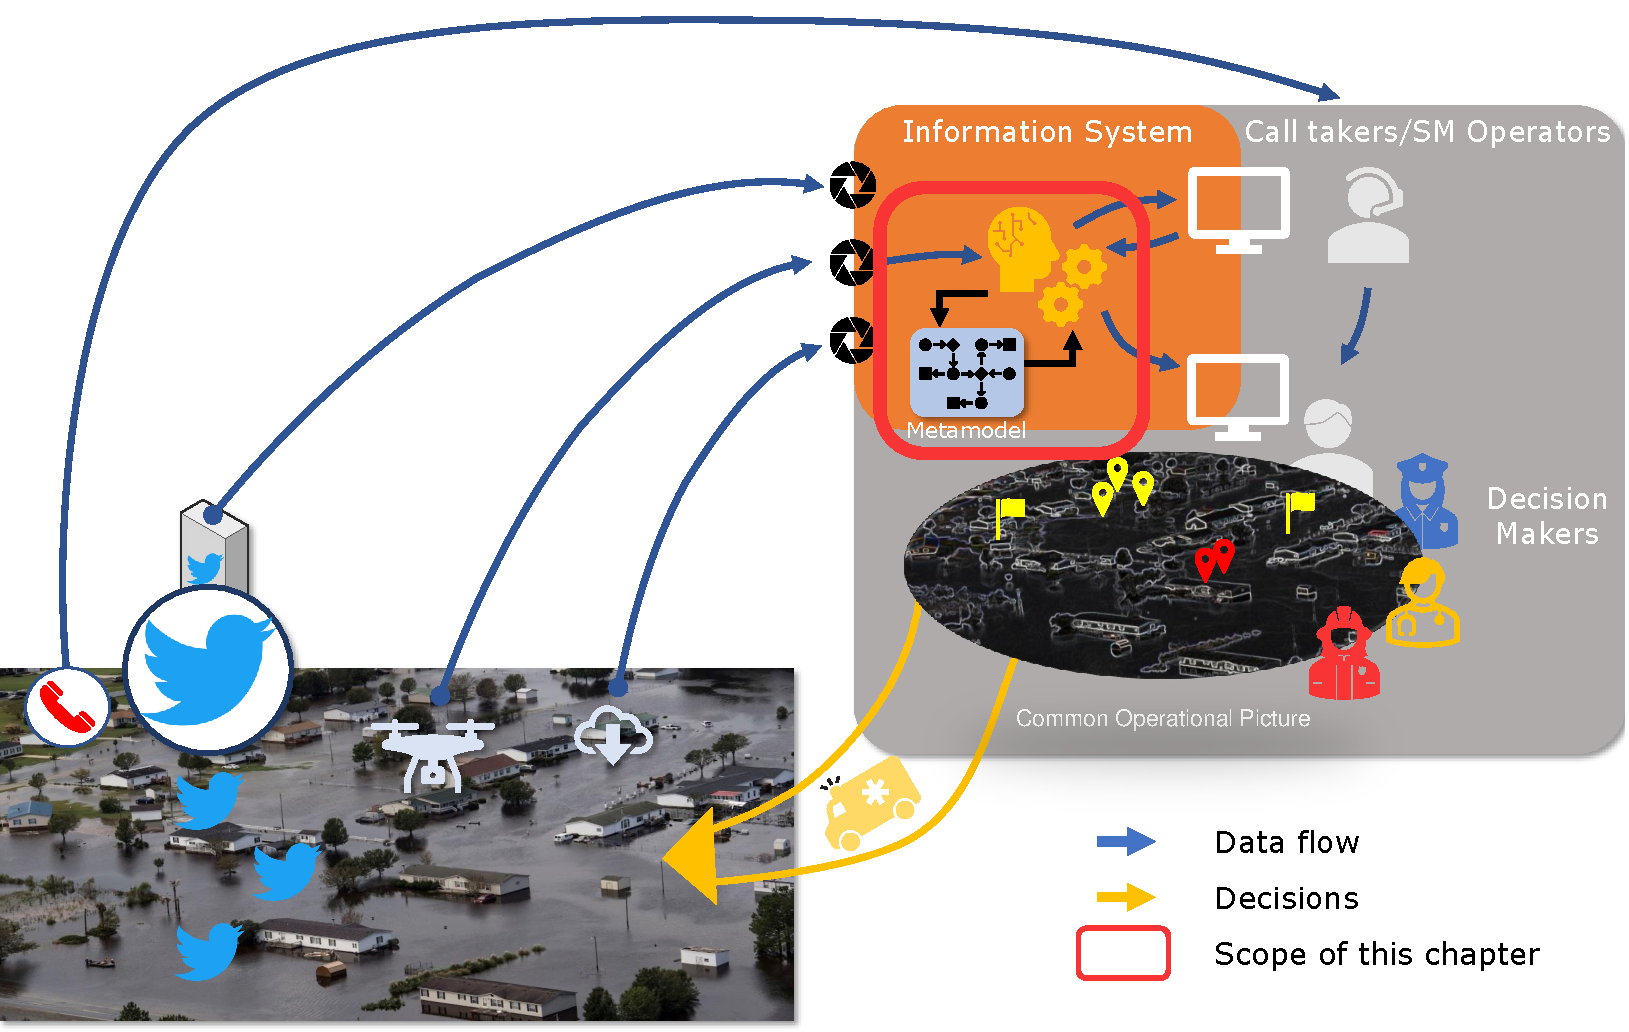
\includegraphics[width=\textwidth]{figures/chap-4/position-chapter.pdf}
    \caption{Location of this chapter in relation to the body of this manuscript.}
    \label{processing:big-picture-manuscrit}
\end{figure}

This chapter presents a new approach to processing social media data to support automatically
the operators in charge of information recovery during disaster response.
This approach aims to gather the information required by decision-makers in the context
of disaster response, i.e., information that fits within the information model presented
at the end of the previous chapter (Figure~\ref{information:information-models}).

This approach is based on machine learning and seeks to identify the information expected
by decision-makers within the messages posted on social media.
Unlike most of the other approaches that process the social media information in this context, the processing is not performed at the scale of the message itself.
Instead, the message is processed at the scale of the different terms that compose the message.
The method relies on previous work realized on this topic to take the processing of the data a step further.
Figure\ref{processing:social-media-processing} illustrates the positioning of our contribution in the light of previous work.
The objective is to facilitate the processing, and thus to save time, on data processing.

\begin{figure}[htb]
    \centering
    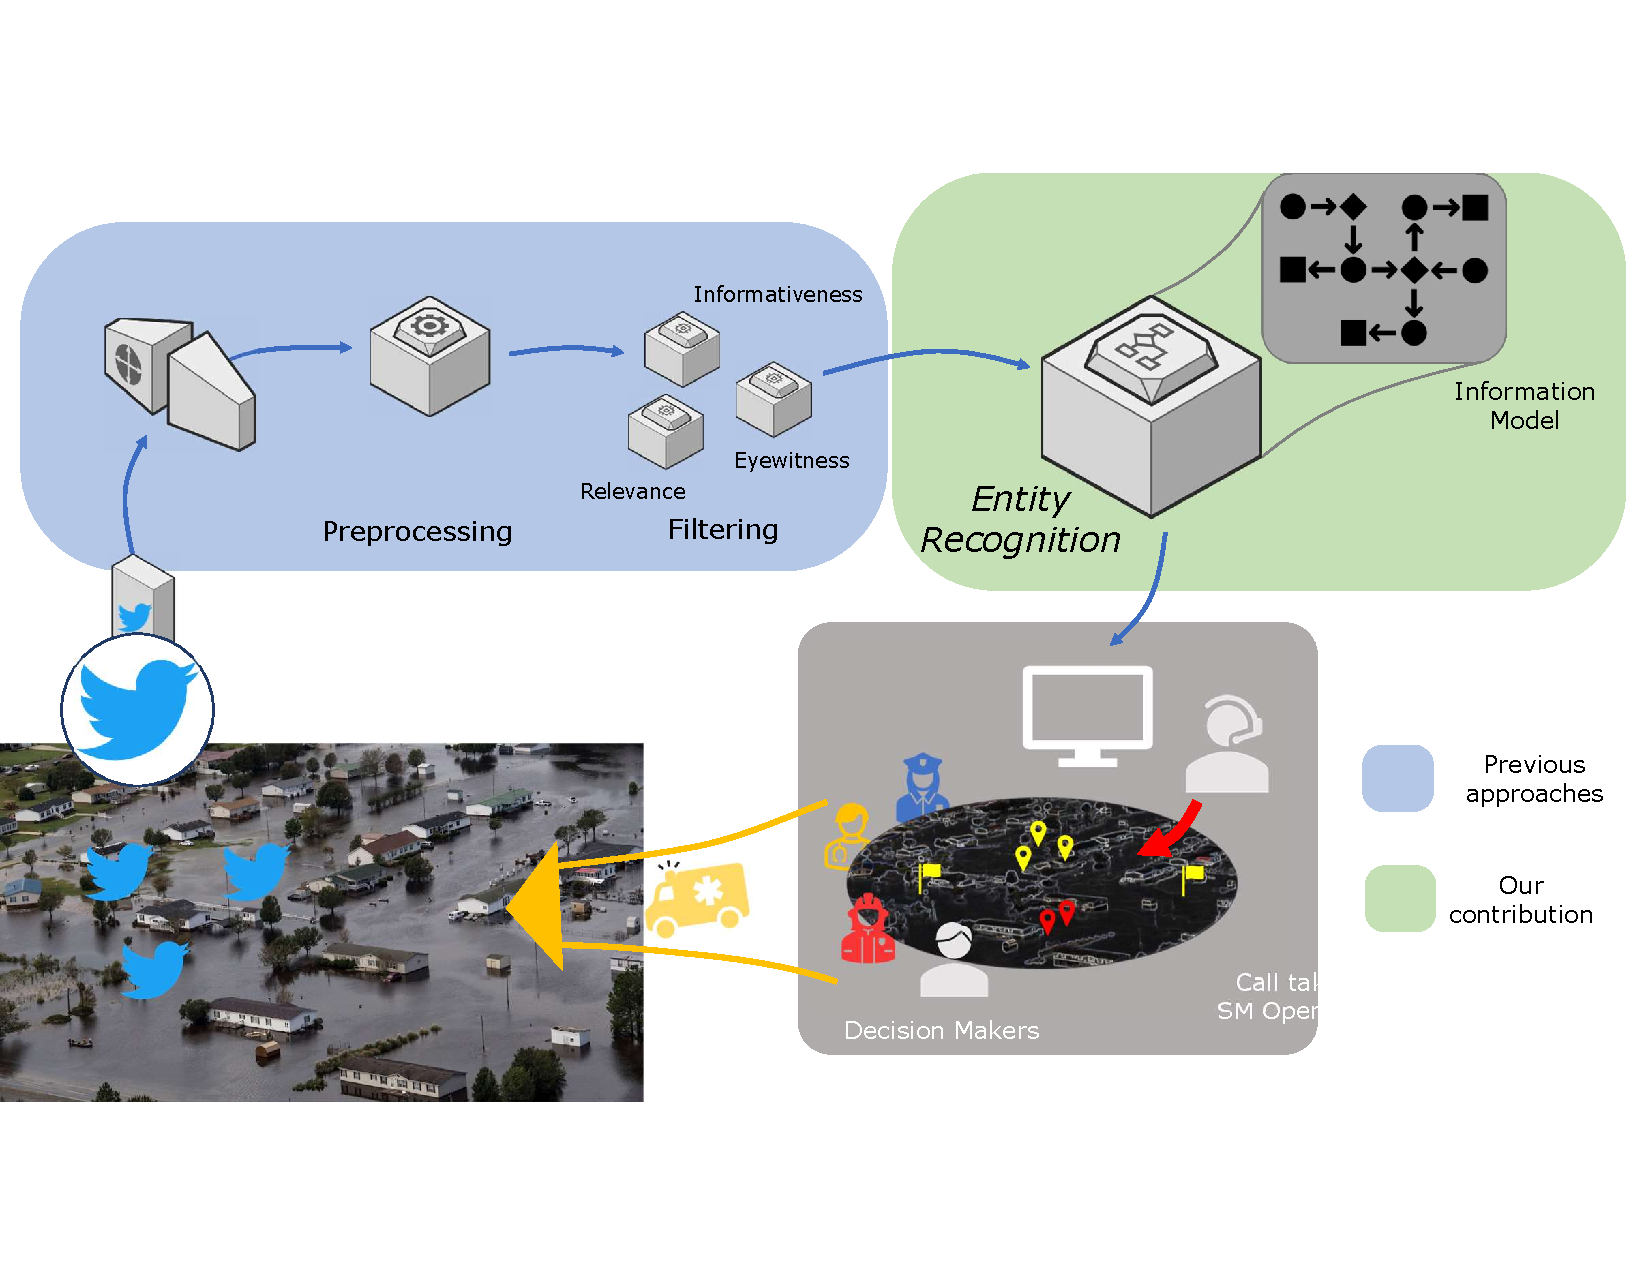
\includegraphics[width=\textwidth]{figures/chap-4/social-media-processing.pdf}
    \caption{Positioning of our contribution with respect to other social media processing tools.}
    \label{processing:social-media-processing}
\end{figure}

The chapter describes in a first section the context of the problem and the constraints
that motivated the design choices for the model.
The second section describes the model and explains the methodology used behind the development.
The last section is devoted to evaluating the model's performance and to the
discussion of the latter in the context of crisis management.

\section{Problem diagnosis}
The previous chapter highlighted the needs encountered by crisis management actors at the
response time.
Specifically, they call for better ways to retrieve their situational awareness and strengthen it, to improve their decision-making.
Among the proposed solutions, we find the idea of sharing actionable information through
a cartographic representation: the Common Operational Picture.
The Common Operational Picture is fed by the information available to each actor, which is then transmitted to
all actors through a common vocabulary or concepts shared by all actors.

However, as also identified in the previous chapter, information retrieval is not performed
by the decision-makers themselves.
Dedicated operators are charged with information retrieval on different information channels
(reports, calls made to the call centers, news, social media, etc.).
The call takers have thus developed frameworks that allow them to obtain information
aligned with the needs of the decision-makers.
Social media, however, due to the high volume of data and the noise/information ratio,
raise new challenges.
The literature review in Chapter 2 highlighted the trend toward automation in crisis informatics.
This trend is intended to reduce the monitoring burden that operators must bear to achieve their results.
In addition, crisis response is usually not an environment that leaves room for insufficiently
effective resources.

The objective is, therefore, to bring together two aspects: (i) processing of social media
that corresponds to the information needs of the decision-makers and
(ii) support in the handling of the volume of data that social media operators are facing.

\subsection{Core problematic}
Social media make available a significant volume of data in the form of text, photos, or videos.
Processing social media content is tedious and harder when compared directly with phone calls.
This is due to the fact that most of the data are unrelated to the current event operators are interested in.
Therefore, they are looking for tools that could help them in their task.

The crisis informatic domain takes on the challenge to provide useful tools that would help in processing social media data.
To reduce the load of the operators, many approaches have been taken.
The first approach consists in increasing the processing capacity through the help of volunteers.
Crowdsourcing tools allow the former to help in the classification of the messages that can then be forwarded to decision-makers \parencite{imranAIDRArtificialIntelligence2014}.
A second approach is to lower the incoming flow of data that the operators are facing.
Some explored ways to reduce the noise part of the flow by filtering messages according to their relevance (linked or not to the ongoing event) \parencite{carageaClassifyingTextMessages2011,imranAIDRArtificialIntelligence2014}.
Others attempted to shrink the incoming flow as a whole by summarizing the information from the incoming data \parencite{rudraSummarizingSituationalTweets2016}.

Emergency responders encounter several problems when they have to process social media.
(i) there is a high volume of data, and (ii) they have to screen each individual message
to extract information, regardless of its interest.

Thus, the solution proposed has to cover two aspects:
\begin{itemize}
    \item It has to reduce the time spent in the processing of incoming messages by reducing the number of unrelated messages and the time spent screening the text to identify relevant information in the flow.
    \item It has to deliver value to the decision-makers by providing the information required by the different actors. The information retrieved should consequently match the concepts used in the Common Operational Picture.
\end{itemize}

The approach presented in this chapter aims to address both aspects.
The contribution builds on previous work that largely addressed the first aspect in
order to address the second part of the problem, which remains essentially unexplored.
The solution proposed in this chapter, and developed in the next parts, highlights the useful entities for decision-makers in the incoming messages.
Therefore, the goal is to highlight in the messages the information that corresponds to
the concepts presented at the end of Chapter 2.

\subsection{Machine learning in disaster response context}
As highlighted in the second chapter, many advances have been realized using machine learning approaches.
These advances greatly benefited natural language processing and provided tools to tackle
new challenges.
However, after time spent with crisis management professionals, one may wonder if
state-of-the-art machine learning models are really suited to the context of crisis response.
There are three inherent aspects of machine learning that one must consider:

\begin{itemize}
    \item The "black box" aspect
    \item The data aspect
    \item The economic aspect
\end{itemize}

Machine learning is, therefore, a toolbox where each tool provides a different way of capturing patterns inherent in data and binding them to the information desired.
An underlying assumption of machine learning is that the patterns present in the data will be repeated in the future.
However, as presented in the first chapter, disasters are by nature unpredictable and are generally similar to a leap into the unknown.
In this context, there is a high degree of uncertainty about the performance of a model trained on data obtained from past disasters.
In the case of a fully unexpected crisis, a system that relies on machine learning can be rendered useless (the returned results are outliers).
The worst-case would be that the system provides erroneous results and that these results are still taken into account by the decision-makers, unaware of the errors.
These aspects are highlighted and discussed by \textcite{endsleyDesigningSituationAwareness2016} and taken up in Chapter 5.
To avoid this scenario, the author recommends including the operators in the functioning of the algorithm by allowing them to influence the results of the algorithm in the most intuitive way possible.

Machine learning approaches consume data to deliver results.
These data can be either labeled or unlabeled.
There exist different algorithms in the machine learning toolbox according to either the
data are labeled or not and correspond to a "learning mode."
The learning is said supervised when the algorithm learn under the supervision of label
example.
It is self-supervised when the algorithm uses raw, unlabeled data to extract knowledge.
An algorithm is said semi-supervised when it uses both labeled and unlabeled data to learn.
All cases require data that need to be gathered.
Labeled data requires the additional data labeling effort.
Self-supervised learning is a specific mode of learning, as it is used to generate language
models, i.e., large vectors that represent the semantic commonly associated with the syllables
found in a language.
The interest and challenges of language models are further developed later in this chapter.
In crisis informatics, most of the approaches use a supervised approach.
The community then gathered datasets of data gathered during several events \parencite{olteanuCrisisLexLexiconCollecting2014,olteanuWhatExpectWhen2015}.
However, these datasets are mostly labeled at the scale of the message itself.
Any work on a different scale, therefore logically requires additional labeling work.
This echoes the generalization problem mentioned earlier, as it is complicated to guarantee
that all the data collected will be representative of the events.
Moreover, any task that would seek to solve a problem occurring at a different scale,
such as labeling the entities present within a sentence, for example, requires a relabeling
of the data.

State of the art machine learning models may require dedicated hardware, especially the
larger models released
Very general machine learning models require adequate hardware and, therefore, a significant investment.
Consequently, running such a model is costly.
The early adopters met during the Early adopter's summit at Charleston in 2020 raised concerns
about the cost of Next-Generation 911.
State of the art machine learning models can require a significant amount of computing
resources.
This is an important consideration when developing a solution to support emergency management centers.
Machine learning is probably the most appropriate tool to solve the identified problem,
but it is important to remember that this tool is not a free lunch.

To summarize, the aim is to facilitate the processing of social media data by highlighting
the information that decision-makers need, i.e., information that is in the information
the model presented at the end of Chapter 2.
Machine learning approaches are indicated to answer this type of challenge.
However, due to the context of disaster response, one has to keep in mind that the solution
i) cannot be a black box to the end-user, ii) has to be generalist enough to be useful in
various situations, and iii) can be run in an emergency center.
A common solution nowadays to the two former constraints is to fine-tune a pre-trained
language model.
This approach associates a good ratio of performance/data labeled and are requiring reasonable
hardware to run.
However, this approach always requires a significant amount of labeled data, representative
of the data that the model will process in the future.
This approach has already been used to classify the relevance of messages posted on social media \parencite{kozlowskiThreelevelClassificationFrench2020}.
However, it is not exactly suited to the context previously described as it does not:

\begin{itemize}
    \item The model act as a black box, as the end-user cannot interact with its results.
    \item There is no labeled data suited for the task
    \item The results provided in case of unseen events are hard to predict.
\end{itemize}

The next sections present a solution that addresses the initial research question while taking
into account the previous limitations.
The first section focuses on the training phase and the second section presents the use
of the method and its performance on an evaluation set.

\section{Scientific foundations of the approach}
The previous problem is similar to a named entity recognition problem.
It seeks to i) locate and ii) label the named entities (brand, person, organization, location etc.) contained in a sentence.
However, instead of looking for named entities, our approach aims to identify predefined
entities, which in our case are the different concepts of the information model.
The proposal is to train a machine learning model in a semi-supervised way able to recognize the entities that belong to the different classes.
The approach relies on two properties of the most recent language models.
First, they allow to "translate" textual data into vectors.
In our case, each word, labeled or not, is associated with a vector.
Secondly, the word vector is obtained from a vector space, whose distance between the different
vectors represents the semantic similarity between the words.
This vector space thus contains clusters of vectors composed of semantically similar entities.
These vectors are obtained by processing the data of the vector space with a clustering algorithm.
It is from this step that the labeled data intervene in the method.
The terms labeled by the operators are included with the other terms.
Therefore, they appear in some of the clusters identified previously.
The labeled terms are used to associate the non-labeled content of the clusters with the labels.
The labels are then propagated from the labeled terms present in a cluster to the non-labeled terms.
In this way, the non-labeled terms semantically close to the labeled terms are associated with the different concepts we are trying to identify.
The different steps of the algorithm are outlined in Figure~\ref{processing:big-picture}.
The method is composed of four main steps after data normalization.
These are:

\begin{enumerate}
    \item Generation of the word vectors associated with each token.
    \item Dimension reduction of the vector space obtained previously to facilitate the following clustering.
    \item Identification of semantic clusters present in the vector space using a clustering algorithm.
    \item Label propagation within the different semantic clusters.
\end{enumerate}

The next sections detail and present the choices that led to the different elements represented.

\begin{figure}[htb]
    \centering
    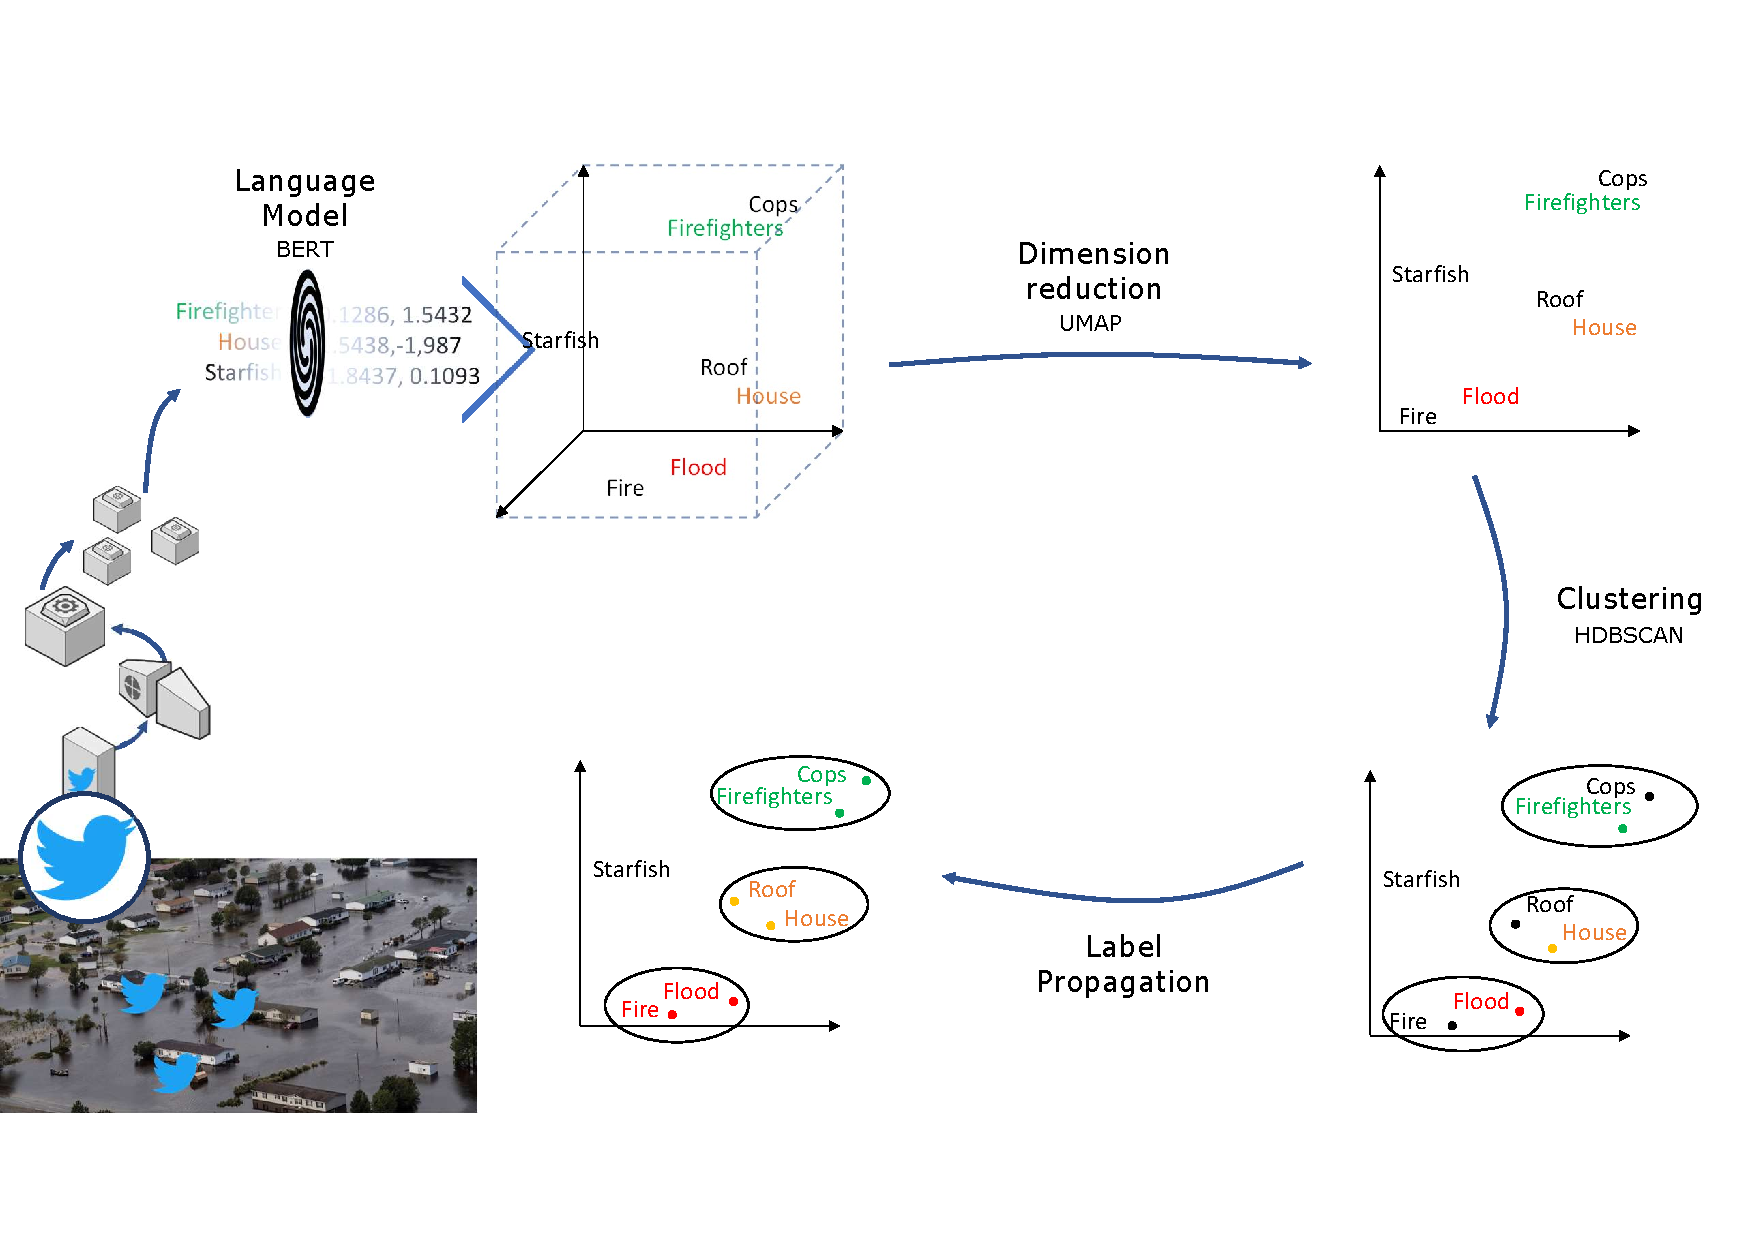
\includegraphics[width=\textwidth]{figures/chap-4/big-picture.pdf}
    \caption{Overview of the approach developped in this chapter.}
    \label{processing:big-picture}
\end{figure}

The semi-supervised approach implies that the training is made using two distinct datasets.
One dataset contains labeled data, and the other contains unlabeled data.
The former, in our approach, contains text messages obtained from previous disaster events.
These messages are sliced to obtain a list composed of the entities that make up the message.
The term "entity" is used here to reflect the fact that, on social media, the message can be composed of other elements than words, like URLs for example.
This process of breaking down sentences is called text tokenization.
Unlabeled sentences are thus broken down into lists of corresponding tokens.
Once all messages are split, a vocabulary is created.
This vocabulary is composed of all the unique entities that are used in the original text messages.
The labeled dataset is composed of words/tokens that are paired with one of the labels of the information.
The two sets of tokens are then merged to create a set of unique tokens, where some are labeled.
The next section presents how language models convert these tokens to vectors that embed the semantic of each token.

\subsection{Language models and semantic representation of textual data}
Texts can be seen as data with two components: a syntactic one and a semantic one.
The syntax composes the form of the text, the graph of the words, and how they combine to create the sentences.
The semantic compose the meaning of the text, the ideas that the text has to convey through a statement.
Computers have many means to process the syntactic part of textual data but lack tools to process the meaning of character strings.
The Natural Langage Processing domain developed different approaches and tools to represent the semantic part of data.
Language models are one of these tools.
They are statistic models that represent the probability distribution over sequences of symbols used to create sentences.
These symbols can be words, letters, or phonemes.
The probability distribution is built assuming that languages have a distributional structure \parencite{harrisDistributionalStructure1954}.
This assumption states that the meaning of a word in a given sentence is provided by the words surrounding it.
The same reasoning is applied at the different scales of symbols mentioned earlier.
Most recent languages models rely on neural networks to construct the probability distribution.
The neural network is trained to predict the probability distribution of words in the different sentences used as training examples.
Instead of producing the probabilities distribution, the distributed representation encoded
in the networks' "hidden" layers are used to represent each word.
Each word is then mapped onto an \(n\)-dimensional vector of reals called a \textit{word embedding}.
Here, \(n\) is the size of the last hidden layer, just before the output layer.
The representations obtained have the distinct characteristic that they model
semantic relations between words as linear combinations.

This approach was popularized with the Word2Vec model proposed by \textcite{mikolovDistributedRepresentationsWords2013}.
Improvements to this method were conducted with models such as GloVe and FastText \parencite{bojanowskiEnrichingWordVectors2016,penningtonGloveGlobalVectors2014}.
Consecutively, attention-based models, able to embed the semantic in longer sentences, appeared.
This new generation of self-trained models is led by architectures such as ELMo, BERT, or GPT \parencite{devlinBERTPretrainingDeep2018,petersDeepContextualizedWord2018}.
Following a similar trend as with Word2Vec, improvements were conducted on this model to increase its performance.
The main differences with this new generation of models are their size (up to hundreds of billions) and their training process.
As explained in the RoBERTa article \parencite{liuRoBERTaRobustlyOptimized2019}, their size makes the training process challenging as they require significantly more training data with a wider variety.
Languages models have also been trained using data specific to a problem, using previously mentioned architectures.
The crisis informatic domain attempted to create crisis-specific BERT models \parencite{liuCrisisBERTRobustTransformer2021}.
However, these models are usually limited by the small amount of data available, in comparison to the volume of data generally used to train this type of model, and this despite the best
collection efforts of the community.
Also, these models are not necessarily made available to the research community, like in the previous reference case, which impedes progress as they are very costly to train.
This approach produces more compact representations, compared to previous methods, whose dimension grows proportionally to the number of unique words contained in the training dataset.
Embedding layers create an arbitrary-sized vector of each word that incorporates semantic relationships.

The proposed method relies on the word embedding of a language model.
The word embeddings are used to produce vectors associated with each token of the set previously created.
These vectors then create a vector space, where the distance between two vectors is equivalent to the semantic similarity between the two vectors.
This property creates a vector space where some vectors, representing semantically close tokens, are spatially close too (see step 1 in Figure~\ref{processing:big-picture}).
The next step is then to identify these "semantic clusters" in the vector space.
This will then allow linking the unlabeled tokens of a cluster to the labeled tokens that are part of the same cluster.
This is achieved by using a label propagation approach within the clusters.
However, while the resulting vector spaces are called "low-dimensional," their dimensions are still too important for clustering algorithms to identify relevant clusters.
Consequently, their dimension is first reduced.
The next section presents the motivation and the algorithm used to perform the dimension reduction.

\subsection{Dimension reduction: UMAP}
The main objective of reducing the dimensionality of a vector space is to avoid facing the
so-called "curse of dimensionality" \parencite{bellmanDynamicProgramming1966}.
This "curse" refers to counterintuitive phenomena that appear in high-dimensional spaces.
For instance, as the dimensionality increases, the volume space increases exponentially.
Thus, data become too sparse, and the notion of distance becomes obsolete.
Dimension reduction is then often used to provide visualizations of high-dimensional spaces.
It consists in transforming data from their original space, to a space of lower dimension.
As this projection necessarily results in information loss, the goal is to find the transformation
that will keep most of the meaningful information.
There are two means (that are often combined) of achieving the projection:
(1) the extraction of the meaningful components and
(2) the projection of the data to a lower-dimensional space.
In practice, most of the algorithms developed to use both approaches.
They first identify or extract meaningful components or representations of the data and then project these to a lower-dimensional space in a way that will preserve most of the original structure of the data.
Among all the available methods and algorithms, the Principal Components Analysis (PCA) is very prominent \parencite{hotellingAnalysisComplexStatistical1933}.
This linear method creates a mapping between the original high-dimensional space and the low-dimensional destination space to ensure minimal loss of information.
The output of the algorithm consists of the vectors used for the linear mapping.
This result is explainable, hence explaining the wide adoption of this method partially.
However, this method shows limitations as the number of dimensions increase.
Indeed, the assumption of the linear distribution of the data becomes less and less correct as of the number of dimensions increases.
As a result, non-linear alternatives have been developed.
Most of these approaches rely on kernels or intermediate representations.
Recently, new approaches based on optimization methods gained significant traction thanks to their ability to provide visualizations that capture the original vector space's global and/or local properties.
For instance, t-distributed Stochastic Neighbor Embedding (t-SNE) uses a low-dimensional
map using probability distributions of data points \parencite{maatenVisualizingDataUsing2008}.
However, t-SNE is only currently capable of reducing to a two or three-dimensional space.
Uniform Manifold Approximation and Projection for Dimension Reduction (UMAP) uses a fuzzy
topological structure to represent the data structure \parencite{mcinnesUMAPUniformManifold2020}.

UMAP can be simplified as a two-step process.
The first one consists of building a weighted topological graph representing the latent structure formed by the vectors in the space of the initial dimension.
The particularity of this graph is that edge weights are not fixed values, but probabilities
that represent the distance instead.
The second step is to transpose the fuzzy weighted graph into the lower-dimensional space.
For this, UMAP builds a new graph in the arrival space in the same way as in the first step.
Creating the best graph in the target space corresponds to an optimization problem where the objective is to find the low dimensional representation with the closest fuzzy topological structure.
Given the setup of the problem, where edges of both graphs are represented using probability distributions, the goal is to minimize the cross-entropy between both probability distributions.
The cross entropy formula takes in two probabilities distributions \(p(x)\) and \(q(x)\),
defined over the discrete variable \(x\), with \( p \in \left\{y,1-y\right\}\) and \( q \in \left\{\hat{y},1-\hat{y}\right\}\)
where \(y\) is the set of input probabilities and \(\hat{y}\) the set of output probabilities.
The formula is given by
\[H(p,q)=-\sum_{\forall x}^{} p\left(x\right) log\left(q\left(x\right) \right)\ = -y log\left(\hat{y}\right) - \left(1-y\right) log\left(1 - \hat{y}\right)\]

Cross entropy allows scoring the difference between the original graph
constructed from the high dimensional data and the constructed arrival graph.
\(p(x)\) is referred to as the true distribution and is represented by the edges obtained from
the original graph.
\(q(x)\) is the distribution of the edges of the arrival graph.
The probabilities of the edges of the arrival graphs are optimized using a Stochastic
Gradient Descent process, which uses the cross-entropy as loss function.

Four main parameters then drive the algorithm:

\begin{itemize}
    \item Number of neighbors: intervenes in the construction of the weighted topological graph and balances the role of the local versus the global structure of the data in the end result.
    \item Minimum distance: represents the minimum distance the algorithm can use between several points (assists in forming dense clusters if needed).
    \item Number of components: the dimensionality of the reduced dimension space in which the data will be embedded.
    \item Distance metric: the distance metric used by the algorithm.
\end{itemize}

The dimension reduction is associated with a compromise left to the user of the algorithm.
Indeed, reducing the dimension of the vectors too much can lead to a significant loss of information.
This compromise also depends on how the reduced dimension space is used.
In our case, it is the grouping of the data into clusters supposed to represent sets of words with similar semantics.
The following section presents, in the same way as for UMAP, HDBSCAN, the algorithm chosen for clustering.

\subsection{Clustering: HDBSCAN}
Clustering consists of grouping sets of data that share similar properties.
This similarity is then represented as the distance between data points.
The representation of data in the form of vectors determines the similarity between data more obvious.
This similarity, or distance, can then be computed as the vector product (or L2 distance) or the cosine between these two vectors.
Many algorithms create clusters of data using different distances.
These algorithms are grouped according to the approach they use to create the clusters.
They can be grouped as below:

\begin{itemize}
    \item the hierarchy (decision tree)
    \item the center of gravity (K-Means)
    \item the distribution of the data (Gaussian mixtures)
    \item the density of the data (DBSCAN/OPTICS)
\end{itemize}

Each approach has its strengths and weaknesses.
Depending on the problem and the objective we want to reach, we will choose one approach.
For example, algorithms based on the centers of gravity often require the number of clusters to be identified.
This assumption is restrictive, primarily when the number of clusters searched is not known a priori.
Thus, other approaches have been developed for the discovery of clusters without a priori knowledge of the number of clusters.
These approaches focus more on the density or distribution of the data to declare the presence of clusters.
Another advantage of this approach is identifying data points that do not belong to any cluster.
In the context of this chapter, clustering is used to identify clusters of tokens that
are close semantically in the vector space created during the previous steps.
The algorithm chosen to perform the clustering on the vector space is Hierarchical DBSCAN (HDBSCAN).
This algorithm is a variant of the DBSCAN algorithm.
The choice of HDBSCAN is made because it is a fast and not greedy clustering algorithm that allows predicting clusters for new points.

HDBSCAN extends DBSCAN with a hierarchical clustering approach where the flat clustering is extracted based on the stability of the clusters.

HDBSCAN works through 5 consecutive steps.
First, it transforms the vector space according to the density of data points.
The core is based on single linkage clustering, which is very sensitive to noise.
The impact of noise is reduced by making sure that noise data points are more distant than those belonging to a cluster.
This is achieved by using the \textit{mutual reachablity distance} between different points
that is given by
\[d_mreach-k (a,b) = \max \left\{core_k (a),core_k (b),d(a,b)\right\}\]
where \(core_k(a)\) is the distance between a point \(a\) and its farthest neighbor among
its \(k\) neighbors.

The mutual reachability distance between the data points is used to generate a graph that connects all the vertices together and with the minimum possible total edge weight.
This graph can be obtained by computing the minimum spanning tree of the graph.
Each data point represents a vertex, and the mutual reachability distance weighs the relationships between the different points.

The minimum spanning tree is used to compute the hierarchy between the clusters.
The edges of the tree are sorted by distance and iterate through each vertex to merge them to a cluster.
These three steps compose the DBSCAN algorithm.
However, the resulting clusters can only be obtained at that stage by setting a threshold at which clusters are defined.
This threshold is a parameter set by the user in DBSCAN that has to define where to "cut" the hierarchy.
This parameter is hard to set in the current situation, as the mutual reachability distance is linked to the density of the cluster.
A better approach is to cut the hierarchy tree at various places to reflect the density difference between the clusters.

The hierarchy tree is then condensed.
Instead of aggregating the data points to form clusters, the problem is turned upside down: we start with a single set that is "losing points" at each split.
To define is points are "lost", the user set a \textit{minimum cluster size}.
If a cluster has fewer points at a split than the minimum cluster size set, then the part with fewer points is dropped off the group, and the part with more points than the minimum is aggregated with the original cluster.
Conversely, if both parts have more points than the minimum cluster size at a split, then two independent clusters are created.
Using this approach, the cluster tree is much smaller than previously.
Using this condensed representation, it is now easier to extract clusters as fewer nodes and splits are in the hierarchy tree.

Just as UMAP, HDBSCAN has a lot of parameters to tune the different parts of the algorithm.
As mentioned earlier, the minimum cluster size is the main and mandatory parameter of the method.
Another parameter of interest is the number of minimum samples.
This parameter intervenes in the creation of the first hierarchy tree and influences the conservativeness of the clustering.
Large values of this parameter lead to more points labeled as noise.
It is tied with the minimum cluster size parameter and takes its value as default.
Other parameters specific to our use case are described in the experimental sections.

HDBSCAN allows identifying clusters formed by semantically close words.
The advantage of this algorithm is that it is very efficient in terms of computation and allows to distinguish efficiently points that are part of a cluster or belong to noise.
Among all the clusters thus formed, some contain some of the words initially labeled by the operator.
The next step is to propagate the labels within these clusters in an ordered way to discover new terms associated with the concepts of the information model.

\subsection{Label propagation algorithm}
The clustering algorithm has identified clusters within the data, which represent semantic clusters whose words have a joint semantic base.
However, there is no way to know to which type of information,i.e., to which label, the different clusters refer.
For this purpose, the words labeled by the operator are used.
As some of these words are located within clusters, they will be used as tags within the cluster, and their associated labels will be propagated to the rest of the cluster.
In this way, it is possible to capture many words that refer to the same concept from a few labeled terms.
Hence, a label propagation approach is used.
This method composes the core of the semi-supervision aspect of our approach.

Label propagation is a method originally designed for graphs \parencite{zhuLearningLabeledUnlabeled2002}.
For a given graph, the idea is to provide a label to some nodes of the graph and to propagate the labels of these nodes until the graph is fully labeled.
The label propagation used here, while following the same logic, is different.
The original method is actually overly aggressive in labeling the data in our setup, where the data are very similar.
To remedy this problem, some improvements have been made.

Propagation takes place within clusters that have at least one label.
Thus, there are two cases:
\begin{enumerate}
    \item There is only one label in the cluster: in this case, the label is simply propagated to all the other tokens in the cluster
    \item Several labels coexist within the cluster.
\end{enumerate}

In the former case, it needs to be controlled.
Indeed, a label should not be propagated on tokens belonging to other labels.
In the same way that we split our starting space into semantic clusters, these same semantic clusters can be split again to identify sub-clusters (referred to as "domains") of different labels.
Once the domains within a semantic cluster are identified, the label propagation is performed similarly to the case where the cluster contains a single label.
This step returns to the case where the cluster is composed of a single label.
This approach mirrors the operation of a K-Means algorithm, which slices a data space into k zones to identify clusters.
The most important parameter of this algorithm is \(k\), the number of clusters present in the data space.
However, the number of domains in a given semantic cluster is unknown at that point.
Therefore, HDBSCAN is reapplied to identify the number of domains in the semantic cluster.
The value of the parameter \(k\) used for the K-Means depends on the number of clusters identified.
Again, there are two cases here: i) there are more labels than domains identified, or ii) there are more (or the same number of) domains identified than labels present in the cluster.
In the former case, the number of domains is passed to the number as \(k\).
The K-Means will then split the space into k partitions which will become our domains.
For each domain that contains a labeled token, the label is propagated to all tokens that are part of this domain.
In the case where the number of labels is equal to or less than the number of identified domains, k takes as value the number of labeled tokens in the semantic cluster.
Each of the labeled tokens is passed as an origin to the K-Means, which then creates the domains around these tokens.
In this sense, each labeled token becomes the epicenter of the propagation of its label within its assigned domain.

In overview, the propagation algorithm is relatively straightforward (see Algorithm~\ref{alg:LP}).
The inputs to Algorithm~\ref{alg:LP} is the set of clusters from the vector spaces that contain at least a labeled word.

\begin{algorithm}[htb]
    \DontPrintSemicolon
    \KwData{A set of $Clusters$ that possess at least a labeled word.}
    \KwResult{The set of original $Clusters$ with their inner labels propagated.}
    \Begin{
        \For{$Cluster \in Clusters$}{
            $NbLabels \longleftarrow GetNbLabels(Cluster)$\;
            \eIf{$NbLabels > 1$}{
                $NbDomains \longleftarrow GetNbDomains(Cluster)$\;
                \eIf{$NbLabels > NbDomains$}{
                    $Domains \longleftarrow KMeans(NbLabels)$\;
                }{
                    $Domains \longleftarrow KMeans(NbDomains)$\;
                }
                \For{$Domain \in Domains$}{
                    $Label \longleftarrow GetLabel(Domain)$\;
                    $PropagateLabel(Domain, Label)$\;
                }
            }{
                $Label \longleftarrow GetLabel(Cluster)$\;
                $PropagateLabel(Cluster, Label)$\;
            }
        }
    }
    \caption{LabelPropagation\label{alg:LP}}
\end{algorithm}

The propagation of the labels within the clusters completes the training phase of the proposed method.
The obtained vector space is now composed of different areas of the space that are labeled.
Overall, the most computational passes are dimension reduction and the first clustering.
Regarding computation time, the label propagation is relatively inexpensive, as the propagation algorithm runs only on the semantic clusters containing labeled tokens.
The next and final section explains how new incoming data are labeled using the vector space created.

\subsection{Inference algorithm}
The trained model is used at response time to highlight relevant entities in messages coming from social media.
Incoming tokens that are already present in the vector space are directly given the associated label.
However, the case of new tokens needs to be handled.

Algorithm~\ref{alg:inference} details the different steps followed.
At first, the incoming message is tokenized, reusing the exact same tokenizer used during the training phase.
Then, the word vector of the token is generated using the language model, and its dimension is reduced using the UMAP model previously trained to map the high dimensional space to the lower-dimensional space.
Similarly, the same HDBSCAN instance is reused to predict a cluster to the incoming token by looking at where the new point would belong in the condensed tree.
Once the cluster has been identified, it remains to assign the corresponding label to the new token.
If the incoming token does not belong to a cluster, it takes its nearest neighbor's label.
If the new token is assigned to a cluster, the situation depends on the number of labels in the cluster.
If there is only one label, the token receives the label of the cluster.
Conversely, if the cluster has several labels, the new token is assigned the label of the nearest word labeled.
When all the tokens of the message are labeled, the message is sent back to the operator with the labels corresponding to each of the tokens of the sentence.

\begin{algorithm}[htb]
    \DontPrintSemicolon
    \KwData{Incoming $Message$.}
    \KwResult{The $Tokens$ of the initial $Message$ labeled.}
    \Begin{
        $Tokens \longleftarrow Tokenize(Message)$\;
        \For{$Token \in Tokens$}{
            $TokenVector \longleftarrow GenerateVector(Token)$\;
            $TokenVectorLow \longleftarrow DimensionReduction(TokenVector)$\;
            $TokenClusterID \longleftarrow PredictCluster(TokenVectorLow)$\;
            \eIf{$TokenClusterID = -1$}{
                $TokenLabel \longleftarrow NearestNeighborLabel(Token)$\;
            }{
                $NbLabelsCluster \longleftarrow NbLabelsCluster(TokenClusterID)$\;
                \eIf{$NbLabelsCluster > 1$}{
                    $TokenLabel \longleftarrow NearestNeighborLabel(Token, TokenClusterID)$\;
                }{
                    $ClusterLabel \longleftarrow GetClusterLabel(TokenClusterID)$\;
                    $TokenLabel \longleftarrow ClusterLabel$\;
                }
            }
        }
    }
    \caption{Inference\label{alg:inference}}
\end{algorithm}

Incoming unknown tokens are then added to the previous ones.
These tokens will also be used when updating the model.
The fast training of the model allows regular updates.
The method greatly benefits from caching, making many of the computations reusable for predictions.
Also, as the number of tokens grows, the number of semantic clusters does not grow linearly.
For example, once the "medical" cluster is discovered, new tokens would just be added to it without necessarily creating a new cluster.

This section presented our method for labeling tokens in social media posts.
It consists of five consecutive steps:
\begin{enumerate}
    \item Normalization of the initial data and extraction of the tokens that compose the vocabulary.
    \item Generation of the word vectors associated with each token.
    \item Dimension reduction of the vector space obtained previously to facilitate the following clustering.
    \item ClusteringIdentification of semantic clusters present in the vector space using a clustering algorithm.
    \item Label propagation within the different semantic clusters.
\end{enumerate}
The proposed approach has the advantage that it uses little labeled data and allows the
operator to adjust the predictions of the algorithm in quasi-real-time.
The following section details the performance of our approach in both qualitative and quantitative terms.

\section{Experimental results}
The proposed approach is evaluated using data coming from datasets used as benchmarks
by the crisis informatics community.
This section presents the testing environment created and the results obtained.
As a reminder, the problem of interest is to label the relevant entities for a crisis operator in a stream of messages from social media.
Therefore, for the evaluation of our method, the efficiency is measured over the labeling of similar content.
The social media chosen here is Twitter.
Twitter allows both easy and wide access to messages posted by users during important events such as natural disasters.
Thus, many datasets related to disasters have been constituted via content posted on this platform.

\subsection{Context of the evaluation}
The experimental setup is designed to create evaluation conditions similar to the initial problem that we are trying to address.
In our case, the goal is to identify relevant entities for decision-making during the response to a crisis event.
The objective is to assist social media operators in their search for information by highlighting the information they need in the messages related to the event.
The support provided consists of filtering the data related/unrelated to the current crisis, then highlighting the information that decision-makers need in the response.
The first part of the filter identifies the relevant tweets—i.e., the tweets refer to the ongoing event.
This part has already seen many contributions, as shown in the literature review.

This experimental part aims at (i) implementing our approach to demonstrate its interest and (ii) evaluating the performances with the chosen algorithmic approach.
Thus, the goal is to identify relevant entities for decision-making in a corpus of tweets already identified as related to the crisis.
The relevant entities chosen for the experiment correspond to the information identified in Chapter 3, which presented some of the information expected by decision-makers during disaster response.
The entities presented were:

\begin{itemize}
    \item Event
    \item Environment
    \item Actors involved
    \item Responders needs
    \item Resource available
    \item Location
    \item Hazard
    \item Equipment
    \item Actors
\end{itemize}

However, this information model is designed to encompass and is not intended exclusively for data or information on social media.
Thus, some of the entities mentioned are hardly present on Social Media \parencite{kropczynskiIdentifyingActionableInformation2018}.
Therefore, the following labels are excluded, for now:

\begin{itemize}
    \item Responders needs
    \item Actors involved
    \item Resource available
\end{itemize}

Identifying Responders' needs requires business knowledge from the decision-maker.
The Resources available can be obtained by subtracting the resources currently in use for the response from the resources allocated to the emergency organization.
Being able to identify if actors mentioned in a text message are involved or not in the response is not doable through the current form of our methodology.
It is, however, a challenging task that requires efforts beyond the scope of this dissertation.
Conversely, our approach is not able to identify entities that relate to location.
The issue of identifying specific and precise locations within a given message has fortunately already been largely explored since many works have been specifically focused on this issue \parencite{pezanowskiSensePlace3GeovisualFramework2018,maceachrenSenseplace2GeotwitterAnalytics2011}.

Thus, the resulting labels used are composed of:

\begin{itemize}
    \item Event — an event that occurs (a car accident, a fire, an earthquake, a person trapped/injured)
    \item Environment — the geographical context where the event takes place (description, how many people are present, the dangers present)
    \item Hazard — a danger that threatens the actors present on an event (a weakened building, a strong water current, a fallen cable)
    \item Actors — Individuals present at the scene of the event. They can be crisis responders, civilians, or victims (victims, firefighters, police officers, doctors).
    \item Equipment — Equipment used in response to the event and which can be used to protect oneself from danger. (a fire truck, safety barriers, a rescue boat, etc.)
\end{itemize}

These six classes correspond to the labels used in the annotation of data for the experimentation.

\subsection{Experimental setup}
\subsubsection{Datasets}
The evaluation of the algorithms calls for various datasets.
On the one hand, the training phase of the model requires the constitution of an unlabeled set of data that will be used to constitute the vocabulary and a labeled set of words of interest.
On the other hand, the evaluation of the model calls for a dataset of labeled tweets at the word level that is as close as possible to real-world application.
The next two subsections present the datasets used, the reason behind these choices, and how they are preprocessed in our case.
%TODO Mettre un mot sur TREC et les versions de BERT etc.

\paragraph{Training data}
The initialization (or training) of the model presented in the previous section relies on two separate sets of data.
The first set, unlabeled, is composed of a vocabulary of terms that will potentially be used to identify entities in incoming text messages.
The second set, labeled, is a set of words of interest for the consumer of the inferences.

The vocabulary is obtained from the CrisisLexT26 \parencite{olteanuWhatExpectWhen2015}.
First, all English tweets are aggregated.
Then the vocabulary was extracted from all previous tweets, i.e., each word used in the dataset was retrieved.
Words that have less than five occurrences are then discarded as they are probably outliers.
The tokenization (segmentation of a sentence into tokens) consists of the following steps:

\begin{itemize}
    \item Usernames are replaced by "@USER"
    \item Links are replaced by "HTTPURL"
    \item Emojis are turned into text using the emoji library\footnote{https://pypi.org/project/emoji/}
    \item Shorten the length of repeated characters
    \item Remove spaces when numbers are involved
    \item Normalization of reduced forms and contractions
    \item Remove punctuation
\end{itemize}

As the tokenization is impacting the performances \parencite[p. 21]{farzindarNaturalLanguageProcessing2017}.
The choice is then made to specify the tokenizer to the format of the data encountered (here tweets).
The second dataset, the words of interest associated with the concepts, is taken from \textcite{olteanuCrisisLexLexiconCollecting2014}.
In this article, the authors suggest a set of keywords to use when querying the Twitter API.
The terms used to constitute the labeled set in the experimentation are derived from this list.
The processing that was done consists of extracting the unique words from this list and removing the adjectives.
The list was then completed by synonyms (especially for buildings) to reach a set of 76 words associated with a concept of the information model.
The constitution of this list, which remains relatively generic, required less than fifteen minutes of labeling work.

\paragraph{Evaluation data}
Evaluating the algorithm's performance requires data that are representative of those that will be provided to the algorithm in reality.
The evaluation, therefore, calls for data that are linked to a crisis, with a certain proportion of noise.
The dataset that will be used for this evaluation is \textcite{zahraAutomaticIdentificationEyewitness2020}.
This dataset is composed of tweets collected during different events (floods, fires, typhoons, earthquakes)
and has been labeled to identify reports from direct witnesses of the event.
However, this dataset is labeled at the message level and not at the word level as we would like in our case.
An annotation phase was therefore conducted to label the words present in the messages.

The annotation was performed using LabelStudio \parencite{tkachenkoLabelStudioData2020}.
It consisted of the annotation of 400 tweets, with 100 tweets taken randomly from each of the listed events.
The disasters studied were: a wildfire, a hurricane, a flood, and an earthquake.
For each event, the proportion of tweets attributed to direct witnesses of the event is 80\%, and 20\% of tweets are considered as not related to the event.
This distribution of data corresponds to the performance presented by state-of-the-art models developed to classify disaster-related tweets \parencite{xukunImprovingDisasterrelatedTweet2020}.
As presented earlier, such a classifier will be used to feed the model with disaster-related messages instead of the raw flow of data.
The data are then labeled using the labels presented in the previous section.
The labeling of the complete dataset took about 4 hours, compared to the 15 minutes to associate the 76 entities to the different concepts.
%TODO Put evaluation dataset on a repo
The data, along with annotation instructions, are publicly available~\footnote{Add link to the data here}.
At the end of the labeling process, 600 words were labeled within the corpus.
The distribution is provided in Table~\ref{table:labels-distribution}.

\begin{table}[bp]
    \centering
    \caption{Distribution of labels among the five classes studied in the test dataset.}
    \begin{tabular}{rl}
        Category    & \# of labels associated \\
        \toprule
        Event       & 434                     \\
        Hazard      & 89                      \\
        Environment & 69                      \\
        Equipements & 5                       \\
        Actors      & 3                       \\
        \bottomrule
    \end{tabular}
    \label{table:labels-distribution}
\end{table}

The distribution of labels within the dataset corresponds to the remark made earlier about
the information available in social media.
Two-thirds of the labels refer to an event, and the remaining labels are mostly found among
two classes — Hazard and Environment.

\subsubsection{Algorithms parameters and language model used}
The language model used to create the vector representations of words is the BERT
model~\footnote{https://tfhub.dev/tensorflow/bert\_en\_uncased\_L-12\_H-768\_A-12/3}.
The UMAP algorithm, used to perform dimension reduction, was configured using the following parameters:

\begin{itemize}
    \item Number of Neighbors: 15
    \item Minimum Distance: 0.0
    \item Repulsion Strength: 1.0
    \item Number of Components: 50
    \item Distance Metric: `cosine`
    \item Number of Epochs: 1000
    \item Learning rate: 0.1
\end{itemize}

This setting aims to force UMAP to focus on the local structure of the data and create clusters that are as split as possible to facilitate HDBSCAN work.
Thus, the \textit{Number of Neighbors} is set to a low value.
Similarly, the \textit{Minimum Distance} is set to 0.0 to pack the data points very tightly.
Inversely, setting the \textit{Repulsion Strength} to 1.0 forces the algorithm to split the clusters it may find.
The dimension is reduced to 50.
This value is a comprise, as a high value will impede HDBSCAN, but a too low value will sacrifice too much information.
Cosine is used to compute the distance between the different vectors, as data are not necessarily normalized.
The \textit{Number of Epochs} and \textit{Learning rate} are linked to the Stochastic Gradient Descent and respectively define the duration of the training and length of each step.

The HDBSCAN algorithm has been parameterized as follows:

\begin{itemize}
    \item Minimum Cluster Size: 15
    \item Minimum Samples: 8
    \item Cluster Selection Method: `leaf`
    \item Cluster Selection Epsilon: 0.0
    \item Distance metric used: `euclidean`
\end{itemize}

Again, the main parameter here is the \textit{Minimum Cluster Size}.
Thus, clusters with fewer than 15 points will be considered as noise.
\textit{Minimum Samples} is linked to the Minimum Cluster Size and is by default set to its value.
It can be seen as the "conservativeness" of the clustering.
Setting a lower value will allow points at the "border" of a cluster to be integrated.
The \textit{Cluster Selection Method} is set to `leaf` instead of the default `excess of mass.`
as it provides better results in the case of a high number of clusters that share a similar amount of data points.
Finally, the distance used here is `euclidean,` as data are normalized for this step.

These parameters are set to maximize the outcome for any type of event.
There is little interest in "fine-tuning" the model in our context, as every situation, hence incoming messages, will be different.
A set of parameters could do exceptionally well on a given dataset but not replicate the performances on another one.
The motivation between these choices is to find a good compromise that should work in the largest number of disaster configurations.

\subsection{Evaluation of the results}
The developed model is studied through a set of metrics that allow evaluating its performances.
Two aspects must be evaluated:

\begin{itemize}
    \item The efficiency of the Named Entities Recognition
    \item The efficiency of the semi-supervised learning
\end{itemize}

The following sub-sections present how they are evaluated in the context of this research.
It is important to note that the evaluation is done as close as possible to the standards of the NLP community.
However, these evaluations ignore the dynamic dimension to which the evaluated algorithms may be subjected.
In the present context, this amounts at best to evaluate the performance of our method at the beginning of the crisis, with generic terms entered by the user.

\subsubsection{NER performances evaluation}
Named Entities Recognition (NER) is a classification problem, and consequently, can be evaluated
using the usual metrics for this type of task: Precision, Recall, and F1-Score.
Precision refers to the fraction of elements correctly labeled among the elements labeled.
The Recall represents the fraction of relevant elements that were retrieved.
Figure~\ref{processing:precision-recall} illustrates both concepts.

\begin{figure}[htb]
    \centering
    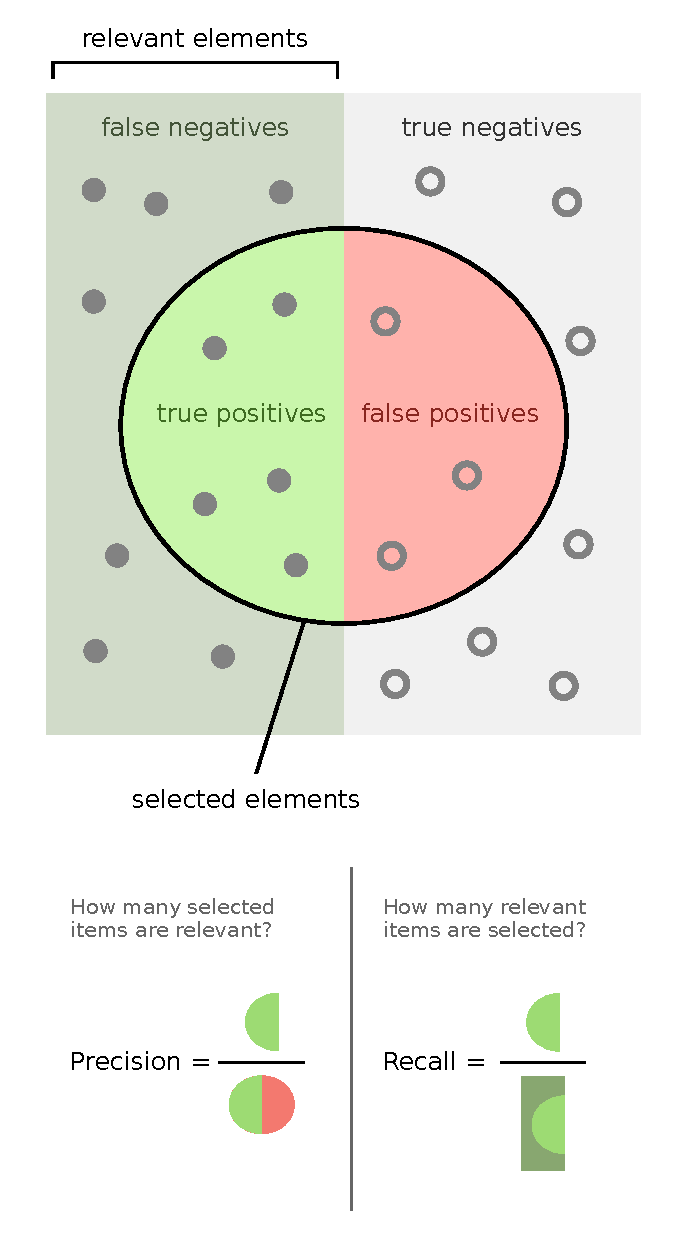
\includegraphics[height=0.5\textheight]{figures/chap-4/precision-recall.pdf}
    \caption{Relation between Precision and Recall.}
    \label{processing:precision-recall}
\end{figure}

The F1-Score corresponds to the harmonic mean of the Precision and Recall.
\[2\cdot \frac{precision\cdot recall}{precision + recall}\]

However, NER evaluation also involves the prediction of the location of the entity in the sentence.
Consequently, there are many ways to obtain results partially correct.
Hence, conferences such as CoNLL defined a variant of the F1-Score better suited for this task \parencite{tjongkimsangIntroductionCoNLL2003Shared2003}.
It redefines the three previous metrics as follows:

\begin{itemize}
    \item Precision is the percentage of predicted entity name tokens that line up exactly with the tokens in the evaluation data.
          If the whole entity is not retrieved by the method, its Precision is zero.
    \item Recall the percentage of entities that appear at exactly the same location in the predictions.
    \item F1 score remains the harmonic mean of the Precision and Recall.
\end{itemize}

\subsubsection{Semi-supervision evaluation}
Semi-supervised learning suffers from a lack of standard evaluation metrics.
Therefore, we propose a set of metrics to evaluate that aspect.
The core of semi-supervised learning is to leverage a small amount of labeled data among a larger volume of unlabeled ones to perform the task.
The first metric to measure the effect of label propagation is the number of entities that have received a label through the label propagation.
This metric allows for the evaluation of the "range" of the label propagation within the unlabeled dataset.
The second metric of interest to evaluate the efficiency of the label propagation on the given problem is to measure how many entities labeled through the propagation have contributed to the final performances.
% Propagation Efficiency = entities labeled through propagation

\subsection{Results}
% ! Évaluer avec différentes seeds.
This section presents the results of the evaluation of the method presented, using the
parameters mentioned and the datasets presented.
First, the performances of the NER are reported, then the performances of the semi-supervision
and finally, the last part is dedicated to the investigation on the performances of the
dimension reduction in the setup.

% ! Faire un avant/après
The Figure~\ref{processing:fire-example} provides a visual of the end result of the method,
where the semantic cluster related to fire is displayed.


\begin{figure}[htb]
    \centering
    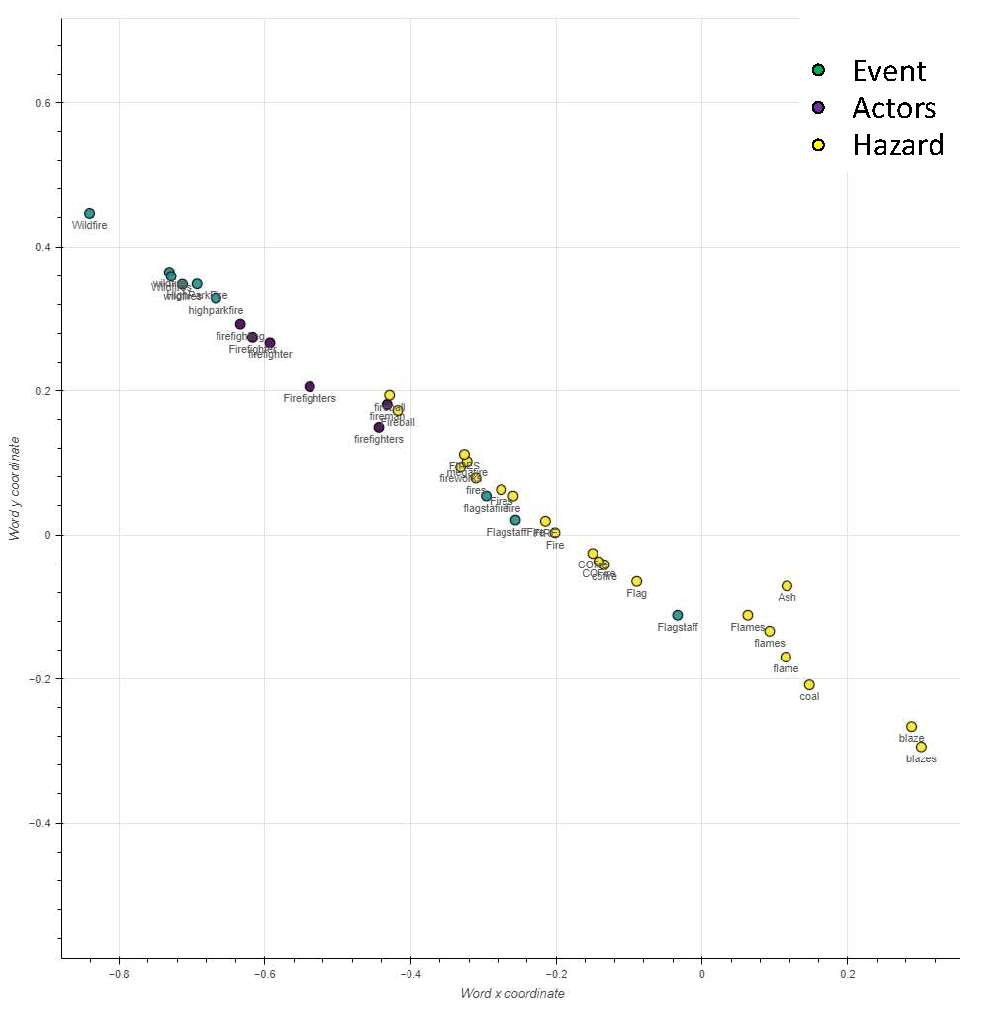
\includegraphics[width=\textwidth]{figures/chap-4/fire-example.pdf}
    \caption{2D projection of the semantic cluster related to \textit{fire} after label propagation. The projection is obtained using UMAP.}
    \label{processing:fire-example}
\end{figure}

% \usepackage[demo]{graphicx}
% \usepackage{subfig}
% \begin{document}
% \begin{figure}%
%     \centering
%     \subfloat[\centering label 1]{{\includegraphics[width=5cm]{img1} }}%
%     \qquad
%     \subfloat[\centering label 2]{{\includegraphics[width=5cm]{img2} }}%
%     \caption{2 Figures side by side}%
%     \label{fig:example}%
% \end{figure}

% ? Comme l'approche s'appuei essentiellement sur des KW, elle renvoit forcément un haut recall.
% ? Ce n'est pas tellement génant dans notre cas, étant donné qu'il s'agit d'un système de support
% ? et non d'automatisation de la prise de décision.
% ? Si quelques entités sont taggés de la mauvaise manière, cela aura peu d'importance d'un
% ? point de vue de l'opérateur.

\subsubsection{NER performances}
% ! Compare with https://github.com/napsternxg/TwitterNER

The performances of our method over all types of events are reported in Table~\ref{table:overall-results}

\begin{table}[bp]
    \centering
    \caption{Results of our method over the four types the events.}
    \begin{tabular}{rcccc}
        Category     & Precision & Recall & F1\-Score & Support \\
        \toprule
        Environment  & 0.220     & 0.652  & 0.328     & 69      \\
        Event        & 0.643     & 0.647  & 0.645     & 434     \\
        Actors       & 0.040     & 0.333  & 0.071     & 3       \\
        Hazard       & 0.263     & 0.764  & 0.391     & 89      \\
        Equipements  & 0.176     & 0.600  & 0.273     & 5       \\
                     &           &        &           &         \\
        weighted avg & 0.531     & 0.663  & 0.565     & 600     \\
        \bottomrule
    \end{tabular}
    \label{table:overall-results}
\end{table}

The performances for each type of disaster are reported as well.
The method obtains its best results on the Event class (see Table~\ref{table:earthquake-results}, Table~\ref{table:fire-results},Table~\ref{table:hurricane-results}) except for the flooding event (Table~\ref{table:flood-results}).
The method performed poorly on the flood event because the labeled terms were not matching the ones used during the event.
However, the same terms applied to the hurricane dataset provided much better performances if one compares both weighted average F1-Score.
The Environment class is partially retrieved over all datasets.
The three remaining classes — Actors, Hazard and Equipements — are harder to evaluate, as there are very little data to explore.
The only significant one is the Hazard class in the fire event, where there are 74 occurrences.
In this case, the model labeled a significant part of the entities correctly.

\begin{table}[bp]
    \centering
    \caption{Result of our method on the data set from the earthquake event.}
    \begin{tabular}{rcccc}
        Category     & Precision & Recall & F1\-Score & Support \\
        \toprule
        Environment  & 0.132     & 0.417  & 0.200     & 12      \\
        Event        & 0.920     & 0.939  & 0.929     & 98      \\
        Actors       & 0.000     & 0.000  & 0.000     & 1       \\
        Hazard       & 0.000     & 0.000  & 0.000     & 5       \\
        Equipements  & 0.000     & 0.000  & 0.000     & 0       \\
                     &           &        &           &         \\
        weighted avg & 0.791     & 0.836  & 0.806     & 116     \\
        \bottomrule
    \end{tabular}
    \label{table:earthquake-results}
\end{table}

\begin{table}[bp]
    \centering
    \caption{Result of our method on the data set from the fire event.}
    \begin{tabular}{rcccc}
        Category     & Precision & Recall & F1\-Score & Support \\
        \toprule
        Environment  & 0.333     & 0.857  & 0.480     & 14      \\
        Event        & 0.651     & 0.719  & 0.683     & 57      \\
        Actors       & 0.071     & 1.000  & 0.133     & 1       \\
        Hazard       & 0.698     & 0.905  & 0.788     & 74      \\
        Equipements  & 0.000     & 0.000  & 0.000     & 0       \\
                     &           &        &           &         \\
        weighted avg & 0.640     & 0.829  & 0.713     & 146     \\
        \bottomrule
    \end{tabular}
    \label{table:fire-results}
\end{table}

\begin{table}[bp]
    \centering
    \caption{Result of our method on the data set from the flood event.}
    \begin{tabular}{rcccc}
        Category     & Precision & Recall & F1\-Score & Support \\
        \toprule
        Environment  & 0.183     & 0.591  & 0.280     & 22      \\
        Event        & 0.291     & 0.228  & 0.256     & 101     \\
        Actors       & 0.000     & 0.000  & 0.000     & 1       \\
        Hazard       & 0.000     & 0.000  & 0.000     & 8       \\
        Equipements  & 0.111     & 1.000  & 0.200     & 1       \\
                     &           &        &           &         \\
        weighted avg & 0.252     & 0.278  & 0.242     & 133     \\
        \bottomrule
    \end{tabular}
    \label{table:flood-results}
\end{table}

\begin{table}[bp]
    \centering
    \caption{Result of our method on the data set from the hurricane event.}
    \begin{tabular}{rcccc}
        Category     & Precision & Recall & F1\-Score & Support \\
        \toprule
        Environment  & 0.250     & 0.714  & 0.370     & 21      \\
        Event        & 0.641     & 0.702  & 0.670     & 178     \\
        Actors       & 0.000     & 0.000  & 0.000     & 0       \\
        Hazard       & 0.015     & 0.500  & 0.029     & 2       \\
        Equipements  & 0.400     & 0.500  & 0.444     & 4       \\
                     &           &        &           &         \\
        weighted avg & 0.590     & 0.698  & 0.629     & 205     \\
        \bottomrule
    \end{tabular}
    \label{table:hurricane-results}
\end{table}

As mentioned in the definition of the metrics used, the results are only a static view of the method.
However, the method does not aim to remain static and is intended to evolve with the situational awareness of the users.
So, while these results provide interesting hints on the model's performance, it does not depict the performances of the model in suitable conditions.

\subsubsection{Semi-supervised learning}

\subsubsection{Influence of the dimension reduction}
An additional experiment has been conducted to test the influence of the dimension reduction to evaluate how this step influences the performances.
All the parameters are kept the same, except that the dimension is never performed anywhere during training or inference.
The results are displayed Table~\ref{table:overall-results-nodim}.
The performances slightly increased, from 0.565 to 0.571 weighted average F1-score.
This version performs better on the Environment category (0.409 from 0.328 weighted average F1-score) and the Event category (0.721 from 0.645 weighted average F1-score).
Notably, there is a trade between the Precision and the Recall in this case.
For the Environment category, Precision went from 0.643 to 0.792 while Recall diminished from 0.652 to 0.275.
A similar trend is observed for the Event category, where the Precision went from 0.263 to 0.862.
The loss of Recall is, however, less severe (from 0.647 to 0.620).
Maybe most importantly, this change in the model made it unable to identify Hazards (0.0 weighted average F1-score) while its counterpart was able to label some of the tokens.

\begin{table}[bp]
    \centering
    \caption{Results of our method over the four types the events.}
    \begin{tabular}{rcccc}
        Category     & Precision & Recall & F1\-Score & Support \\
        \toprule
        Environment  & 0.792     & 0.275  & 0.409     & 69      \\
        Event        & 0.862     & 0.620  & 0.721     & 434     \\
        Actors       & 0.000     & 0.000  & 0.000     & 3       \\
        Hazard       & 0.000     & 0.000  & 0.000     & 89      \\
        Equipements  & 0.500     & 0.200  & 0.286     & 5       \\
                     &           &        &           &         \\
        weighted avg & 0.719     & 0.482  & 0.571     & 600     \\
        \bottomrule
    \end{tabular}
    \label{table:overall-results-nodim}
\end{table}

These results call for more investigations on this aspect, but it hints that different models may perform differently based on the dimensions fed to the clustering algorithm.

\section*{Conclusion}
This chapter presented a novel approach to process social media, based on machine learning, that aims to be used in disaster response situations to provide the information expected by decision-makers.
The first part discussed the context of disaster response and how it influences the processing of social media data.
In particular, the use of machine learning in this context was discussed, highlighting both the advantages and disadvantages of such an approach.

The second part of this chapter presents the model itself, details the functioning of its different parts and the motivation behind the choices made.
The resulting algorithm is composed of 4+1 steps:

\begin{enumerate}
    \item (Data normalization and tokenization).
    \item Generation of the word vectors associated with each token.
    \item Dimension reduction of the vector space obtained previously to facilitate the following clustering.
    \item Identification of semantic clusters present in the vector space using a clustering algorithm.
    \item Label propagation within the different semantic clusters.
\end{enumerate}

As of today, there is little evidence that traditional machine learning approaches are suited for such context.
Consequently, the model is designed to allow quick adaptation of the results to fit as much as possible to the ongoing event.
In a sense, the model aims to fit the context, not the data provided initially.
The overall composition of the model is then designed with practicability in mind over raw performances.

The last section of the chapter explored the performances above.
The attempt was to explore the different aspects of the approach and quantify their impact on performances.
Improvements can be thought for several aspects of the model.
Right now, the approach is very limited to the fact that it considers the tokens independently.
However, this issue can be solved by considering the surrounding tokens through a window sliding over the sentence.
Another aspect linked to label propagation is that semantic clusters of interest that do not contain a labeled word are currently ignored.
This aspect represents an exciting avenue for future work.
I want to emphasize that the evaluation of machine learning models, or other related systems, using the standard practices of the NLP domain, can hardly evaluate the true performances of these systems in the context of disaster response.
Evaluation on a given, the fixed dataset does not represent the unexpected and evolving nature of the problem they try to address.
\textcite{halseSimulatingRealtimeTwitter2019} proposed a tool to simulate a stream of tweets from a dataset based on message sending information.
If this tool was originally designed for training social media operators, an adapted version could be used to test machine learning algorithms dynamically.
This area remains open to contributions that will undoubtedly yield important outcomes for crisis management organizations.
Finally, the algorithm presented here has only solved a sub-part of the initial problem.
The objective of automatically retrieving information from social media cannot by itself answer the initial challenge.
Improving disaster indeed asks for better decision-making of the different actors involved.
Similarly, improved decision-making requires better access to quality information.
However, if decision-makers informational needs might help improve the quality of the information delivered, the accessibility falls out of scope.
As described in the previous chapter, information retrieval is rarely performed by the decision-makers themselves but more often by dedicated operators.
Hence the final research question: \textit{How should be organized social media processing systems in disaster management situations?}
The next chapter explores the challenges and possibilities in the design of an information system for disaster response.

%%% Local Variables:
%%% mode: latex
%%% TeX-master: "../ma-these"
%%% End:


\chapter*{Decision Makers}

\section{Partie technique}
Section qui repond à la question : Comment met on en oeuvre concretement la solution apportee precedemment ?
Notre solution est un systeme d'aide à la decision sense fonctionner durant des evenements de crise.
Les systemes d'aide a la decision viennent avec des contraintes supplementaires par rapport du fait de leurs systemes de recommendations.
Il faut maintenir un niveau acceptable de qualite pour les recommendations.

En plus de cela, il est important de prendre en compte les contraintes liees a la gestion de crise, à savoir :
\begin{itemize}
    \item Fortes contraintes sur les ressources (humaines particulierement)
    \item La solution finale doit etre cheap
\end{itemize}

Liste de ressources pour alimenter cette partie :
\begin{itemize}
    \item Introducing MLOps
    \item Machine learning Engineering
\end{itemize}


\section{Partie design}
Partie finale de la these.
Elle repond a la question : Comment est-ce qu'on fait pour delivrer les resultats de la these au preneur de decision ?
Pour ce faire, on propose de s'interesser à l'UI et l'UX du SI, et notamment la COP qui sera proposee au decision maker.
Plus precisement, comment est-ce que les suggestions faites par le systemes permettent de prévenir les daemons de la SA mentiones par Endlsey.
Liste des ressources utiles pour alimenter cette partie :
\begin{itemize}
    \item https://pair.withgoogle.com/guidebook/chapters
    \item https://pair.withgoogle.com/guidebook/patterns/how-do-i-get-started
    \item Les SA daemons de Endlsey
\end{itemize}


%%% Local Variables:
%%% mode: latex
%%% TeX-master: "../ma-these"
%%% End:


\chapter*{Conclusion and Perspectives}

The response to a crisis is strongly influenced by the ability to make the right decision at the right time.
However, the reality of the crisis makes this objective more remote and often forces compromises.
In the hope of reducing the gap between reality and the objective, many actors have sought to improve information feedback to decision-makers.
This work is part of that effort, seeking to serve content posted on social media to the people who need it.
However, many challenges are emerging.
Social media is not the only source of data to feed decision-makers situational awareness.
Faced with this influx of data and information, it is essential to limit as much as possible the extra and limit the mental load attributed to this task.
This observation only increases the status of the information system (IS) in crisis management.
The IS becomes responsible for taming the torrent of data, extracting information that it must then organize and provide appropriately.
This vision has guided all of the previous work, the main contributions of which are summarized in the following.

\section{Summary}
The first chapter of this dissertation presented its scientific background composed of three domains: (i) crisis management, (ii) social media, and (iii) natural language processing.
This Ph.D. research works were conducted at the intersection at both of these domains and identified the principal research question that guided the rest of the document: \emph{How to design an information system for crisis response that can automatically manage and deliver actionable information from social media data?}

The second chapter provided an overview of previous works on the different aspects of the research question.
It highlights the coexistence of two fields around these issues: information sciences and social sciences. Each field explores the space of the problem and meets at certain intersections.
This part also shows the important interest of the scientific community for the automatic processing of social media content and the work to implement it in crisis management.

In this context, the third chapter asks what information decision-makers need from social media.
Once this information is identified, it needs to be represented in a computerized way to automate its organization and collection.
The information science community has proposed numerous computer representations, or information models, for crisis management.
The last part of this chapter presented an information model for the information available on social media for decision-makers.
This model is obtained by intersecting the needs identified in the first part with the relevant information models identified in the second part.

The fourth chapter builds on the earlier information model to propose a method for automatically identifying this information.
This method builds on previous work that seeks to differentiate between messages related to the event and those that are not.
The processing among the resulting messages is similar to the recognition of named entities, with the difference that the entities are not named but correspond to actionable information.
This identification is performed using a machine learning method.
Training the machine learning model in a supervised fashion raises challenges in the context of crisis management.
Hence, a semi-supervised approach is preferred for training the model.
The latter is based on the word embeddings created by a language model such as BERT.
The dimension of the vectors provided by BERT is then adopted to identify the clusters of terms present in the dataset provided as input to the algorithm.
Some of these clusters contain terms that the user has previously labeled according to the actionable information of the model.
The labels of these terms are then propagated to all the other unlabeled terms present in the cluster.
In this way, the terms labeled by the user and their synonyms are highlighted in the incoming message flow.

Finally, the fifth and last chapter considers the IS as a whole.
In particular, it asks about the role and issues of integrating the data processing method into an IS for crisis management.
After studying the literature on the associated issues in the first part, it is concluded that such an IS is composed of two parts.
One part is dedicated to managing data, which are used in part to feed the AI at the heart of the IS.
A second part is responsible for information management and considers user input and output.
Another aspect of the proposed dichotomy is the distinction between data and information storage.
The first case is carried out with the help of a traditional relational database.
Information storage is based on the association of an information model, such as those mentioned above, and a graph-oriented database.
The graph database allows defining instances of the information present in the model and semantic relations between the different cases.
This approach promises many evolutions in processing information exchanged during a crisis.

\section{Perspectives}
The work presented in this document covers a rather large area of study by trying to mix human and technical around this scientific challenge.
However, at the dawn of this document, more questions remain unanswered than answers have been given.
This field of research remains rich and challenging, both scientifically and technically.
The following parts present potential research directions that I currently foresee.

\subsection{Short terms}
The problem of misinformation and fakes was mentioned in Chapter 1 of this dissertation.
Although excluded in this work, this issue is more than ever decisive for the success of social media-based modules.
\textcite{batardIntegrerContributionsCitoyennes2021} mainly refer to beneficial citizen initiatives in his work.
However, the opposite behavior is also observed.
Some citizens may actively use social media to share ideas or ideologies detrimental to crisis management.
The results obtained around this issue must now be integrated into systems.
Their objectives would be to detect and fight more upstream against potential trends that could harm the response.
This problem remains a significant issue for many practitioners who regularly mention it as a deterrent to adopting such systems.
This integration would reassure them and thus facilitate adoption and experimentation.

Additionally, it would be interesting to consolidate the proposals made on specific issues on the technical aspects.
Topics well discussed should free up space for suggestions concerning new uses of the data and feedback on these technologies.
Such a topic could be the classification of messages evoking an event.
The most effective suggestions could now be consolidated to allow use by practitioners.

\subsection{Mid-long terms}
A better understanding of the expectations and needs of practitioners, especially when dealing with unique situations, would also be very beneficial.
A large volume of publications takes a top-down approach, proposing solutions directly to users.
However, many of the observations made by the practitioners reveal and reflect their difficulties and needs.
Better integration and collaboration between domains would necessarily lead to better results for crisis management.
Practitioners who are among the early adopters are key players.
Their feedback and testimonies save precious time searching for appropriate solutions to the issue at hand.

This document also mentioned the numerous data sources that can support crisis management.
Messages posted on social media and photos or videos are all information accessible from social media.
However, other sources have been mentioned, such as video streams from drones or readings from various sensors.
The collection and automatic interpretation of these data is currently the focus of scientific attention.
This results in a large amount of information being generated through the interpretation of the data.
This heterogeneity is an asset, and many developments are to be expected thanks to it.

A future challenge will be to homogenize the available information to exploit its full potential.
Such homogenization is made possible by a standard information model that allows the standardization of information obtained from different sources.
Two direct consequences are expected.
First, using several sources allows for different incidents or different geographical areas.
Thus, someone can report an event in progress in an area not covered by a camera or vice versa.
This consequence corresponds to an extension of the information or the \emph{horizontal} scaling of the coverage.

This heterogeneity also allows for vertical scaling.
Having different data sources covering the same event can provide additional information than a single source.
For example, someone can warn via social media that an event is taking place, and a camera on the spot can better understand the context and type of event concerned.
This application thus corresponds to an \emph{enrichment} in information.
This enrichment can also take place on the same information.
For example, a user indicates an event has taken place and mentions a location.
At the same time, a surveillance camera also detects an event at this exact location.
The concordance of these two pieces of information reduces the uncertainty of some information.
Providing an indicator of certainty in the information proposed by the system would also reduce the mental load on decision-makers.

%%% Local Variables:
%%% mode: latex
%%% TeX-master: "../ma-these"
%%% End:


\appendix

\chapter{Appendix A}

\begin{landscape}
    \begin{figure}
        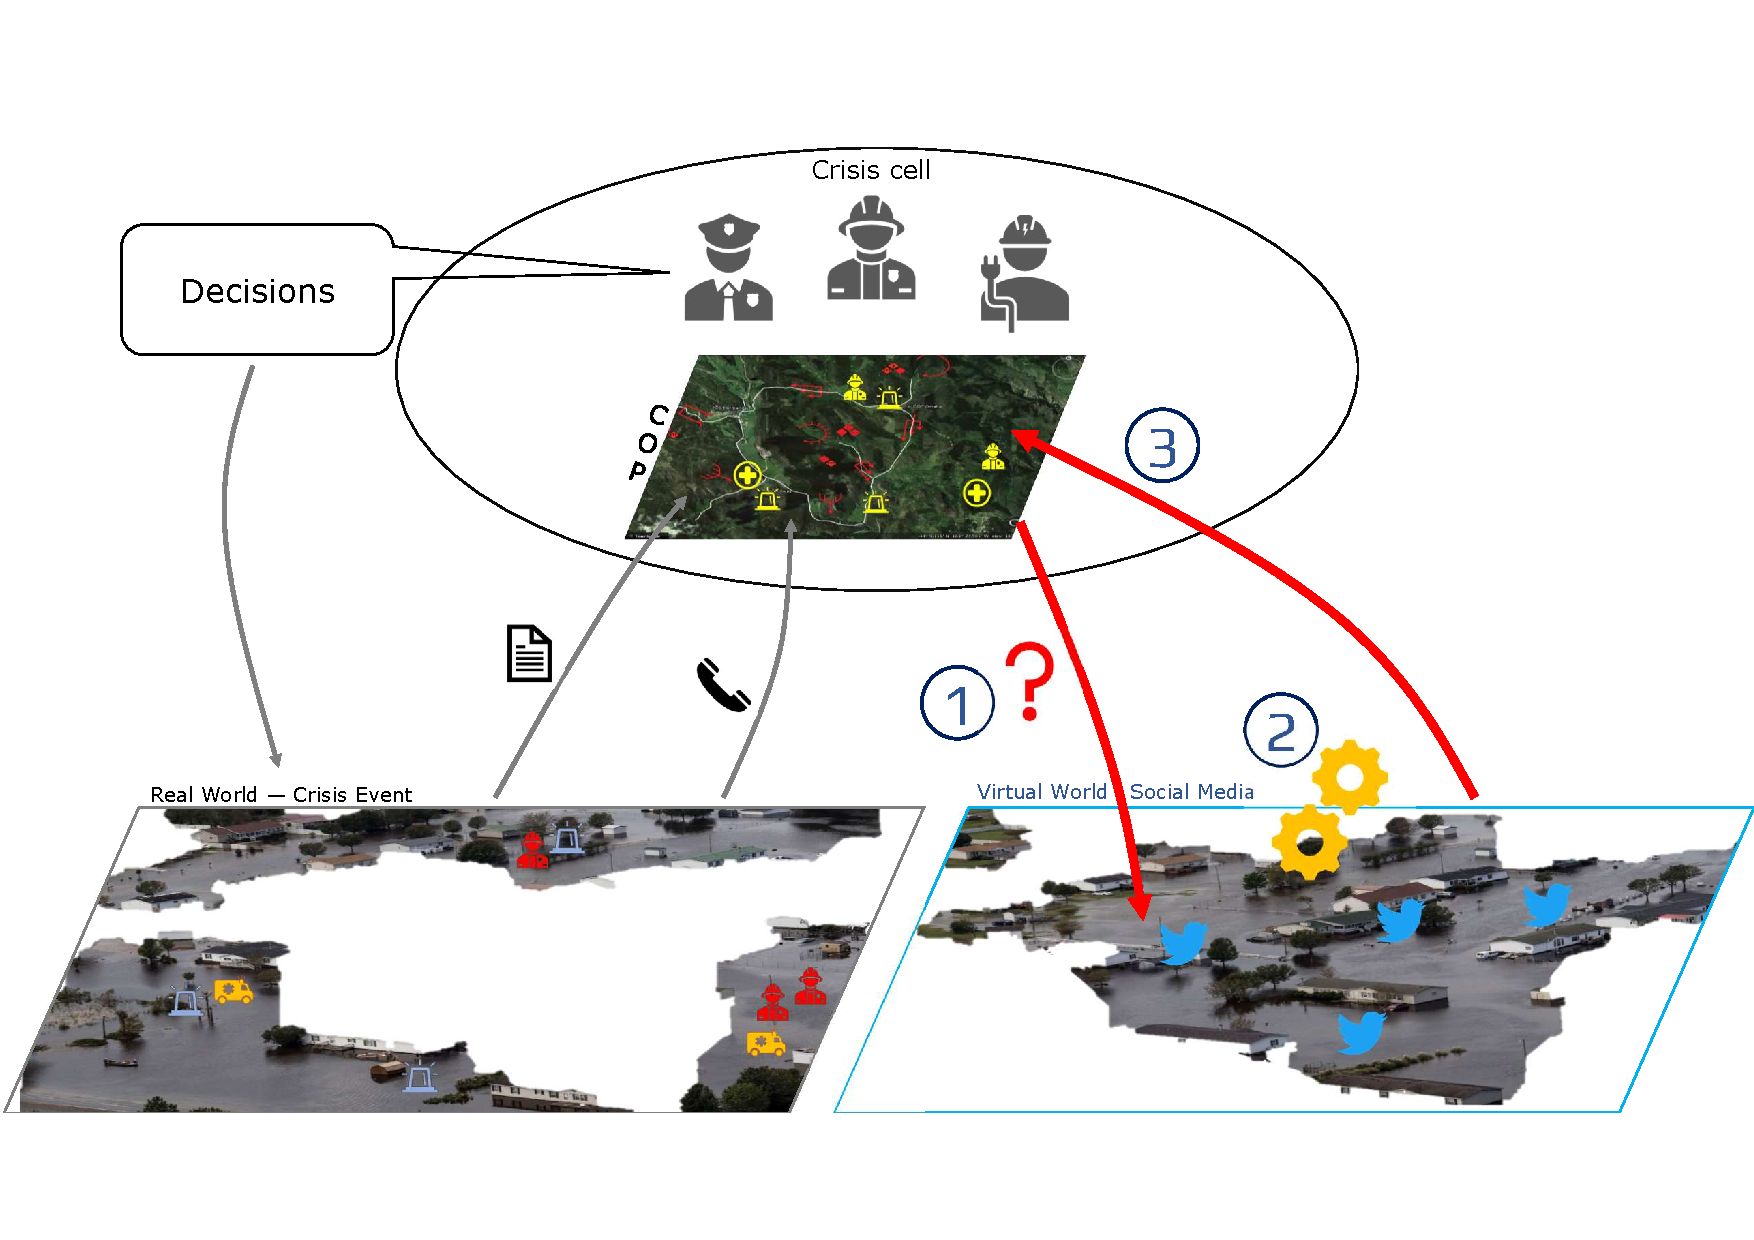
\includegraphics[width=\paperwidth,height=\paperheight,keepaspectratio]{figures/big-picture.pdf}
        \caption{Formal representation of the Information model presented Chapter 3 using the UML 2.0 langage.}
        \label{information:information-models-uml}
    \end{figure}
\end{landscape}

%%% Local Variables:
%%% mode: latex
%%% TeX-master: "../ma-these.tex"
%%% End:


% \chapter{Une seconde annexe}

Ici, le contenu de la seconde annexe...

%%% Local Variables:
%%% mode: latex
%%% TeX-master: "../ma-these"
%%% End:


%----------------------------------------
\backmatter

\listoffigures

\listoftables

% \listofsymbols % la nomenclature

% Les acronyms
% {
%   \renewcommand*\glspostdescription{\matmdotfill}
%   \printacronyms[style=list,nogroupskip]
% }

% la bibliographie
\printbibliography[heading=chapter]

\tableofcontents

% le résumé (en 4e de couverture)
\cleardoublepage
\pagestyle{empty}
\null
\newpage
\abstract[0.6]%
{french}{Résumé}%
{Conception d'un système de traitement des médias sociaux en réponse de crise : extraction, gestion et distribution des informations pertinentes pour les décideurs.}%
{
  Nos sociétés ont toujours été ponctuées de situations de crises, mais la complexité croissante de ces
  événements exige une amélioration constante des méthodologies et des outils employés lors de la réponse.
  L'établissement d'une conscience de la situation commune à tous les acteurs impliqués est l'une de ces améliorations
  potentielles.
  Cependant, cette axe d'amélioration souffre de difficultés liées au manque de ressources à allouer à cette tâche.
  L'automatisation d'une partie des tâches pour supporter le personnel en charge de cet aspect, est donc une opportunité de recherche.
  Cette opportunité est également favorisée par le développement des médias sociaux en tant que sources de données massives.
  Simultanément, le domaine de l'intelligence artificielle a été radicalement modifié par
  le développement de nouveaux outils et de nouvelles méthodes, permettant la recherche
  d'informations complexes au sein de données textuelles.
  À la croisée de ces trois opportunités conjugués, cette thèse explore la question suivante :
  Comment concevoir un système d'information capable de gérer et de fournir automatiquement
  des informations pertinentes extraites des données des médias sociaux ?

  Une approche en trois temps est proposée. Premièrement, il s'agit de comprendre
  quelles sont les informations pertinentes lors de la phase de réponse à une crise pour les preneurs de décision.
  Deuxièmement, une fois les informations pertinentes identifiées, un nouveau module d'intelligence
  artificielle dédié extrait les éléments pertinents à partir des données disponibles sur les médias sociaux.
  Ces informations sont alors intégrées dans un modèle de situation de crise, permettant
  de les organiser automatiquement avec le reste du contexte.
  La troisième et dernière partie discute de l'organisation des données et
  des informations au sein d'un système d'aide à la décision pour la gestion de crise.
  Cette discussion s'intèresse particulièrement à la question de la bonne gestion et de
  la distribution de ces informations auprès des décideurs.
  Cette recherche a été menée dans un contexte international : le projet français ANR
  MACIV, une collaboration entre IMT Mines Albi et Penn State University et en relation
  étroite avec des praticiens français et américains.

  \keywords{Mots-clés :}{Gestion de crise, Apprentissage Machine, Traitement Automatique du Langage, Connaissance de la Situation, Système d'information}
}
{american}{Abstract}%
{Design of a social media processing system for crisis response: extraction, management and delivery of relevant information for decision makers}%
{
  Our societies have always been punctuated by crises, but the increasing complexity of these events requires a constant improvement of the methodologies and tools used in the response.
  Establishing a common situational awareness among all actors involved is one of these potential improvements.
  However, challenges arise due to the lack of available resources to allocate to this task during crisis response.
  The automation of certain tasks to support teams' dedicated actionable information collection, therefore, represents a research opportunity.
  This opportunity is also enabled by the expansion of social media as big data sources.
  At the same time, the field of artificial intelligence has been radically changed by the development of new tools and methods, allowing the retrieval of complex information within textual data.
  At the crossroads of these three opportunities, this dissertation explores the following question:
  How to design an information system capable of managing and automatically providing relevant information extracted from social media data?

  A threefold approach is proposed.
  The first part aims at understanding what information is relevant in the crisis response phase for decision-makers
  Second, once the relevant information is identified, a new, dedicated artificial intelligence
  module extracts the relevant elements from the data available on social media.
  This information is then integrated into a crisis model, allowing to automatically
  pair it with associated information available in the context.
  The third and last part discusses the organization of data and information within a decision support system for crisis management.
  This discussion is particularly interested in designing a system that can achieve proper management and distribution of information to decision-makers.
  This research was conducted in an interdisciplinary context: the French ANR MACIV project, a collaboration
  between IMT Mines Albi and Penn State University and in close relationship with French and American practitioners.

  \keywords{Keywords:}{Crisis Management, Machine Learning, Natural Language Processing, Situation Awareness, Information System}
}

%%% Local Variables:
%%% mode: latex
%%% TeX-master: "../ma-these"
%%% End:


\end{document}

%%% Local Variables:
%%% mode: latex
%%% TeX-master: t
%%% End:
